\documentclass[12pt, a4paper, titlepage, openany]{book}
\usepackage[utf8]{inputenc}

\usepackage{courier}
\usepackage{wrapfig}
\usepackage{verbatim}
\usepackage{quotchap}
\usepackage{graphicx,eso-pic}
\usepackage[explicit]{titlesec}
\usepackage[font={small,it}]{caption}
\usepackage{indentfirst}
\usepackage{ragged2e}
\usepackage{hyperref}
\usepackage{tabu}
\usepackage{amssymb}
\usepackage[dvipsnames,table]{xcolor}
\usepackage{amsmath,tikz}
\usepackage{enumitem}
\usepackage{soul}
\usepackage[most]{tcolorbox}
\usepackage{tabto}
\usepackage[nottoc,numbib]{tocbibind}
\usepackage[english]{babel}
\usepackage[titles]{tocloft}
%\usepackage[framed,numbered,autolinebreaks,useliterate]{mcode}
%\usepackage{python}
\usepackage{minted}
\usemintedstyle{fruity}
\usepackage[top=2cm,bottom=2cm,left=2.5cm,right=2.5cm,headsep=20pt,a4paper]{geometry} 


\setlength{\footnotesep}{0.5cm}
\graphicspath{{../Graphics/}}
\definecolor{ehone}{RGB}{8, 63, 77}
\definecolor{ehtwo}{RGB}{7, 54, 66}
\definecolor{ehthree}{RGB}{42, 161, 152}
\definecolor{ehfour}{RGB}{0, 43, 54}
\definecolor{ehfive}{RGB}{32,244,254}
\hypersetup{colorlinks=true,linkcolor=ehfour, urlcolor=ehone}
\renewcommand{\cftdot}{}
\raggedbottom

\input Kramer.fd


\newcommand\chapterimage[2][]{%
  \AddToShipoutPictureBG*{% Add picture to BackGround on this page only
    \AtTextUpperLeft{% Position at upper left of text block
     \hspace*{\textwidth}% Move over to upper right of text block
      \llap{% Ignore horizontal width and overlap to the left
        %\smash{% Ignore vertical height
          %\raisebox{-\height}}% Include image with options

%------------------------------------------------------------------------

\begin{document}
\frontmatter
\begin{titlepage}
\color{ehone}
\fontsize{60pt}{72pt}\usefont{U}{Kramer}{xl}{n}
\noindent THE \\ ENTROPYHUB \\ GUIDE\\ 
\vspace{5mm}
\normalfont		
   \begin{center}
    \Large
	\noindent \textbf{\textit{A user manual for the EntropyHub toolkit}} \\
   \end{center}
 
\vspace{7cm}
\begin{wrapfigure}{r}{0.25\textwidth}

\includegraphics[width=1\linewidth]{EntropyHub_profiler.png} 
\label{fig:wrapfig}
\end{wrapfigure}

\normalsize 
\noindent \textbf{Matthew W. Flood}	
\newline \\ \newline
\noindent \href{https://www.EntropyHub.xyz}{\ul{\textbf{www.EntropyHub.xyz}}} 
\newline \\ \newline
\noindent \textbf{v.2.0 (2024)}

%\date{\today{}}	% The \today function uses the current date.
\normalsize
\color{black}
\end{titlepage}




\thispagestyle{plain}
	
%\vspace*{\fill}
\footnotesize

	\begingroup
	  \begin{center}	 
	  \vspace*{4cm} 
		
\includegraphics[scale=.75]{EntropyHubLogo3.png}	\\	
		\vspace*{\fill}
	  \textbf{Copyright 2021, Matthew W. Flood}\\ \ \\ \
		\end{center}	   
	
	  \noindent Licensed under the Apache License, Version 2.0 (the "License");
	   you may not use this file except in compliance with the License.
	   You may obtain a copy of the License at \\	   
	
	       http://www.apache.org/licenses/LICENSE-2.0\\
	
	   \noindent Unless required by applicable law or agreed to in writing, software
	   distributed under the License is distributed on an "AS IS" BASIS,
	   WITHOUT WARRANTIES OR CONDITIONS OF ANY KIND, either express or implied.
	   See the License for the specific language governing permissions and
	   limitations under the License.\\
	   
	   \noindent See Terms of Use at www.EntropyHub.xyz\\ % License information
		
	\endgroup

\normalsize
	


\begin{savequote}[100mm]
  
\qauthor{ }
-- I prefer to take the names of important scientific quantities from ancient languages, so they may be the same in all living languages. \\I therefore propose to call \textbf{entropy} the quantity (S) of a body  from the Greek word for transformation: $\eta$ $\tau\rho o\pi\eta$
\qauthor{Rudolf Clausius}
-- Quantities of the form $H = -\Sigma\ p_i\ Log\ p_i$ play a central role in information theory as measures of information, choice and uncertainty. The form of \emph{H} will be recognized as that of \textbf{entropy} as defined in certain formulations of statistical mechanics where $p_i$ is the probability of a system being in cell \emph{i} of its phase space. H is then, for example, the H in Boltzmann's famous H theorem.\\
We shall call $H = -\Sigma\ p_i\ Log\ p_i$ the \textbf{entropy} of the set of probabilities \  $p_1, \dots, p_n$.
\qauthor{Claude Shannon}
-- The fact that you can remember yesterday but not tomorrow is because of \textbf{entropy}. The fact that you're always born young and then you grow older, and not the other way around like Benjamin Button - it's all because of \textbf{entropy}. So I think that \textbf{entropy} is underappreciated as something that has a crucial role in how we go through life.
\qauthor{Sean M.Carroll}
\end{savequote}


\chapter*{\vspace{10cm}\textbf{Preface}}
\chapterimage[width=16cm, height=3cm]{Chapter Banner2.png}
\vspace{1cm}
The concept of entropy has its origins in \href{http://www.scholarpedia.org/article/Entropy}{classical physics} under the second law of thermodynamics, a law considered to \href{https://www.penguin.co.uk/books/301539/the-order-of-time/9780141984964.html}{underpin our fundamental understanding} of \href{https://en.wikipedia.org/wiki/Time_in_physics}{time in physics}. Attempting to analyse the analog world around us requires that we measure time in discrete steps, but doing so compromises our ability to measure entropy accurately. Since the introduction of approximate entropy by Pincus three decades ago\footnote{Steven M. Pincus, \\\indent\indent \emph{Approximate entropy as a measure of system complexity},\\\indent\indent Proceedings of the National Academy of Sciences (1991);  88.6: 2297-2301},
the use of information theoretic entropy measures to estimate the complexity, randomness or regularity of time series data has become ubiquitous in many research domains (Fig. \ref{fig:fig_1}a). Applications of entropy are ever-increasing (Fig. \ref{fig:fig_1}b), as are the number of new entropies that aim to estimate entropy with greater accuracy, less sensitivity to data length, amplitude fluctuations, etc. (see Ribiero et al.\footnote{Ribeiro M, Henriques T, Castro L, Souto A, Antunes L, Costa-Santos C, Teixeira A., 
\\\indent\indent \emph{The Entropy Universe}, \\\indent\indent Entropy (2021); 23(2):222})

\vspace{5mm}
\begin{figure}[!ht]
    \centering
	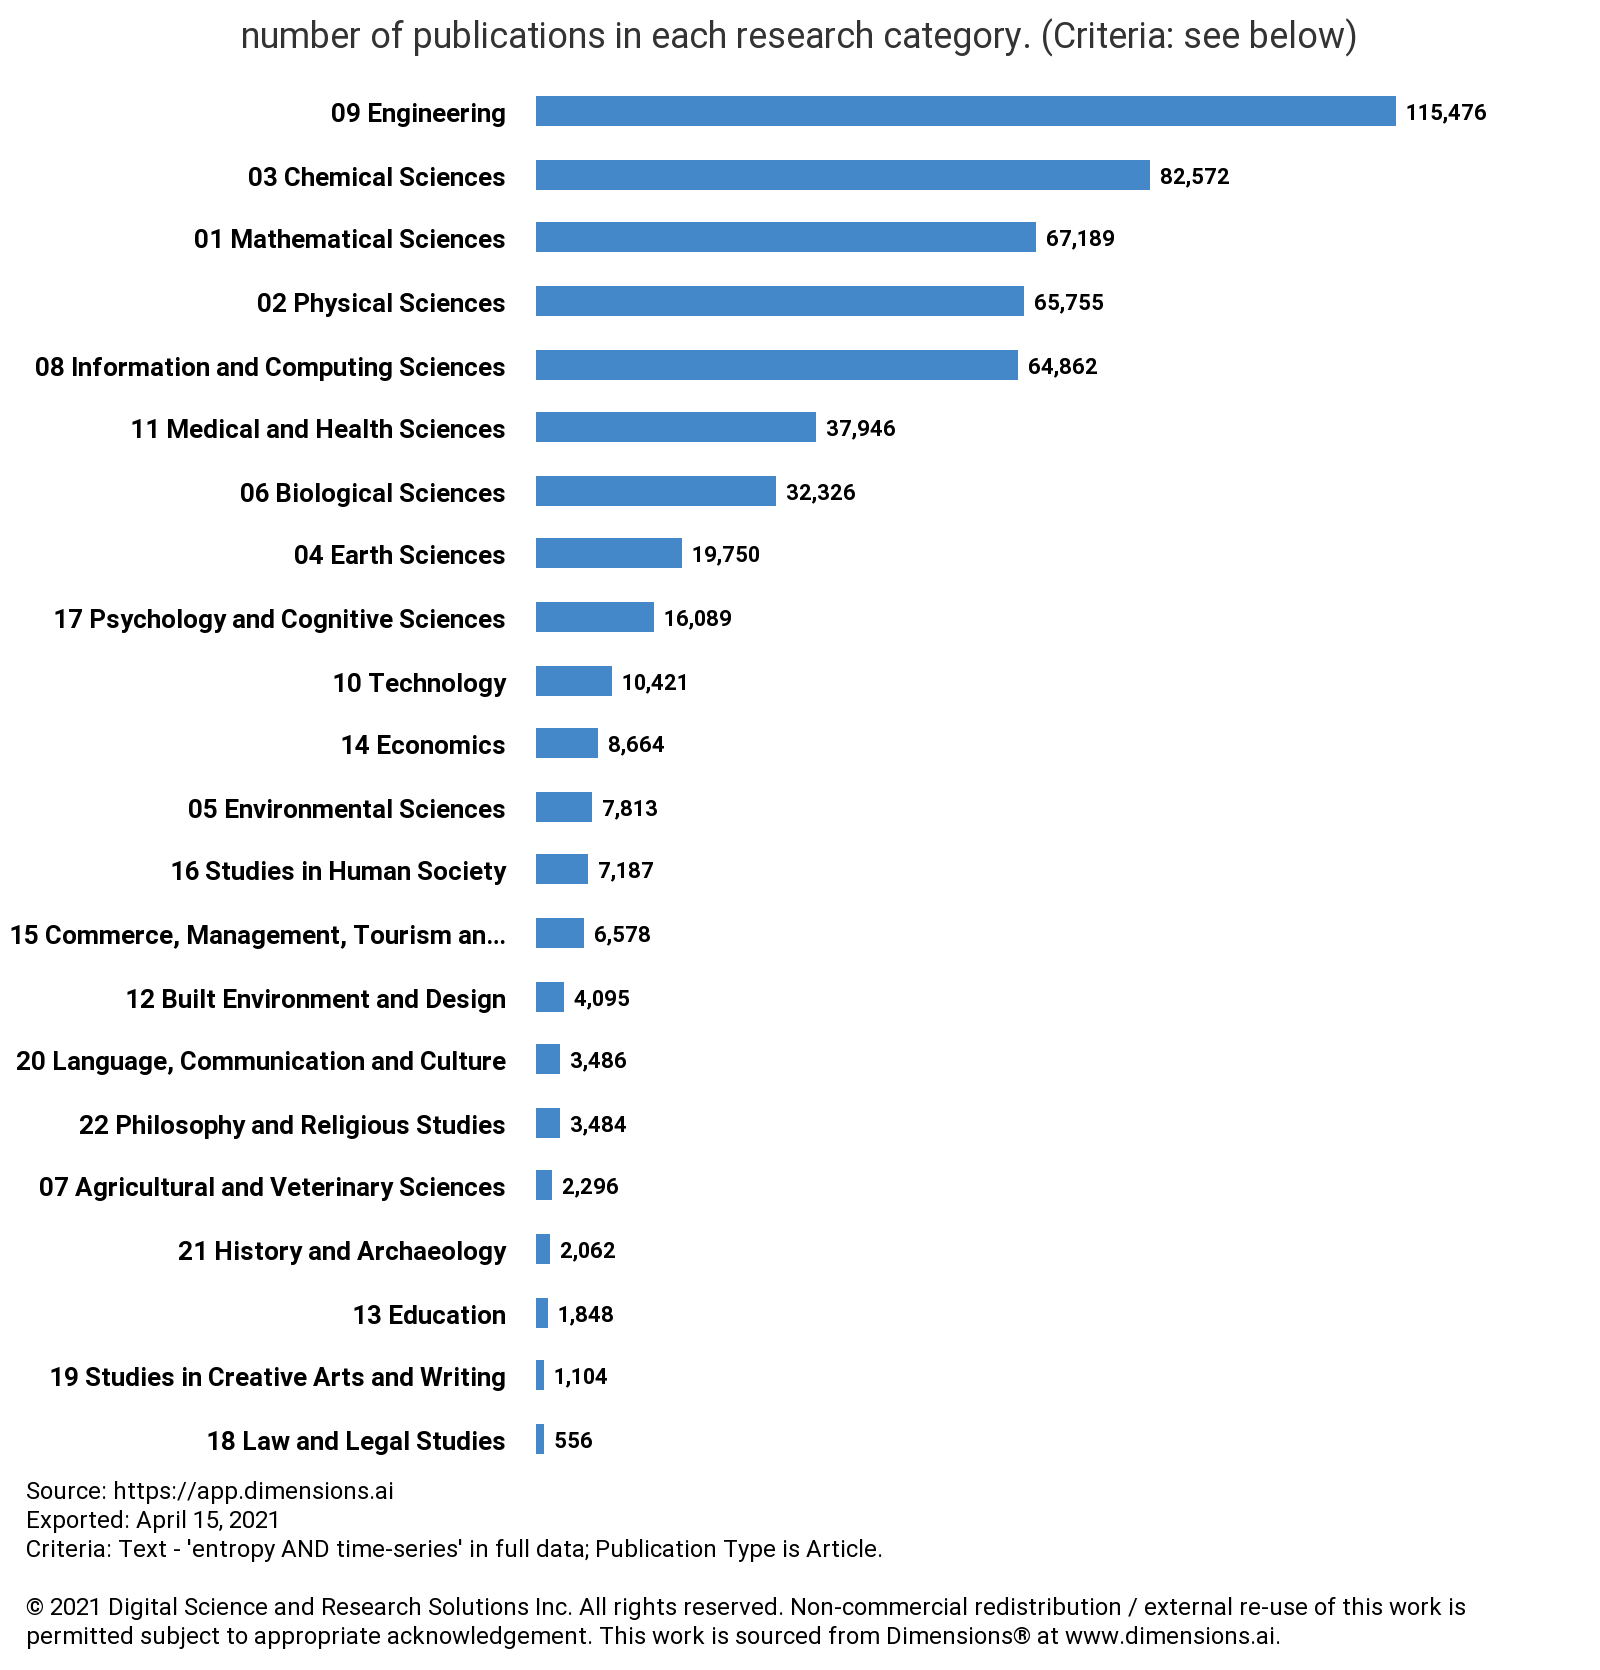
\includegraphics[scale=.175]{Preface2.png}
	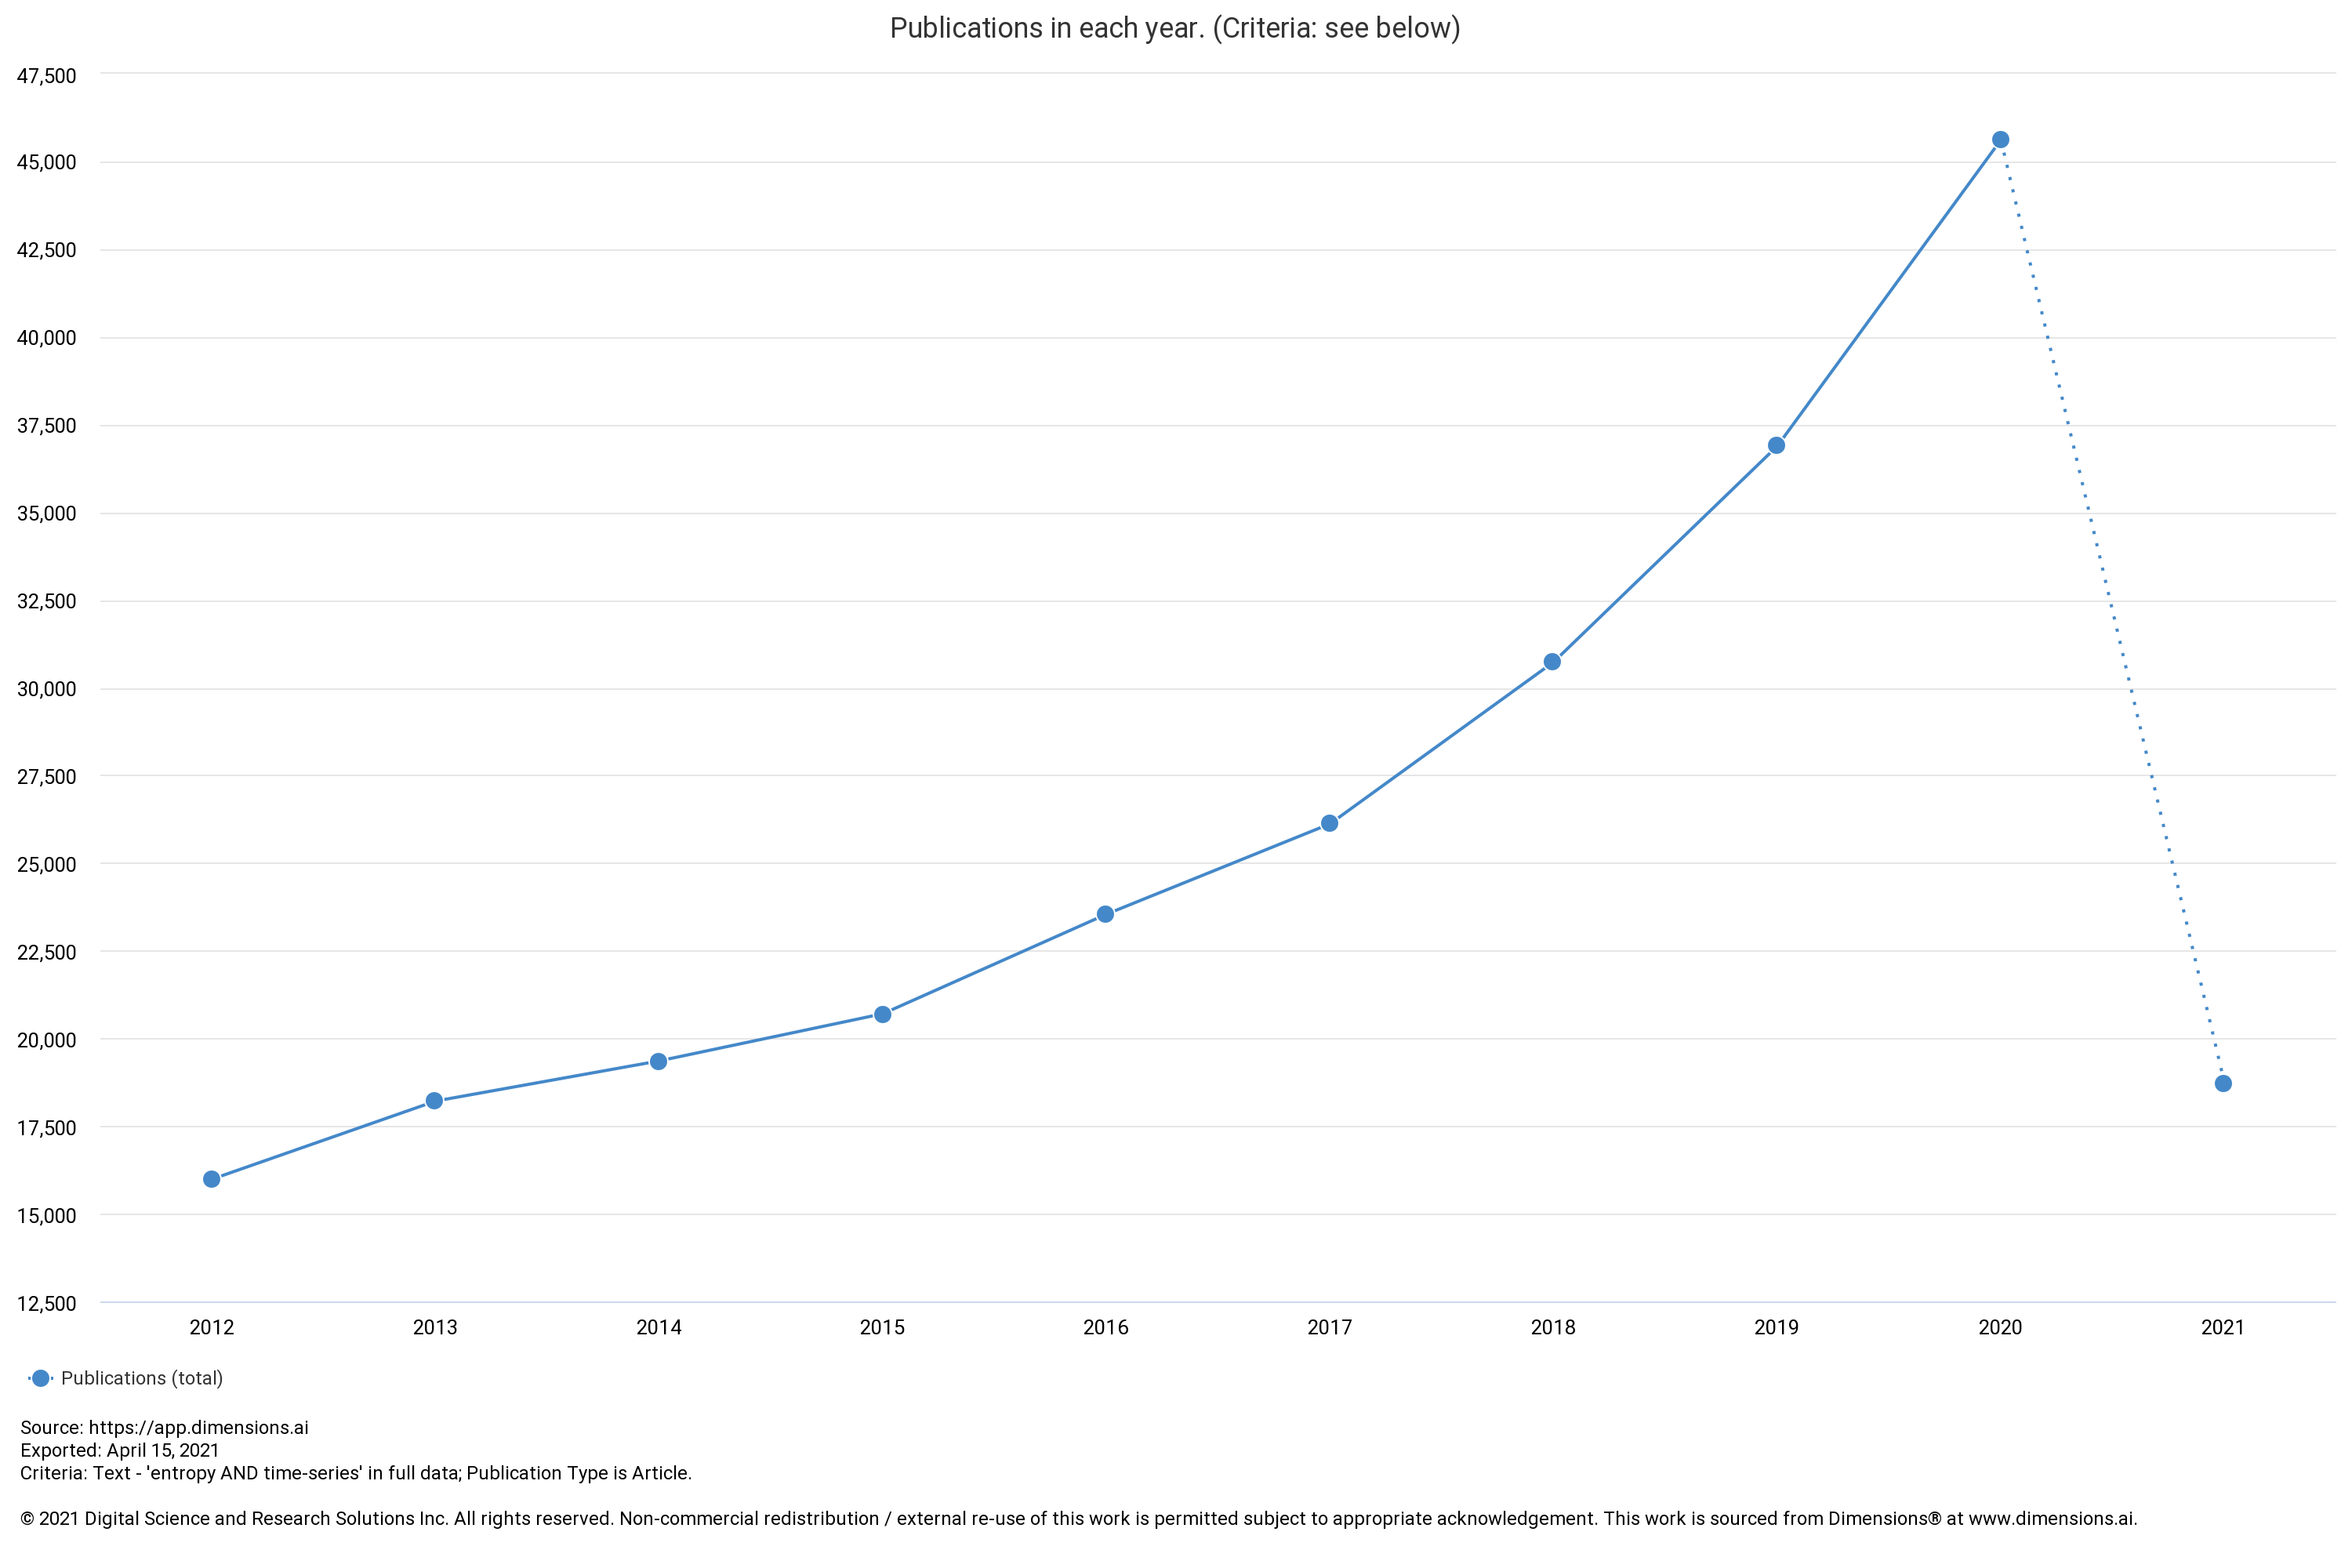
\includegraphics[scale=.15]{Preface1.png}
    \caption{Research domains and the number of publications each year featuring the terms \emph{'Entropy' AND 'Time-Series'} from 2012-2021. (\textit{Source: Dimensions.ai})}
    \label{fig:fig_1}

\end{figure}

Although many functions for estimating these entropies can be found in various corners of the internet, there is currently no toolkit to perform entropic time-series analysis at the command line with reliable code, extensive documentation and consistent syntax, that is also accessible in multiple programming languages. Hence, the goal of EntropyHub is to integrate the many established entropy methods into one package that is available for users of Python, MatLab and Julia.

\vspace{5mm}
EntropyHub features multiscale variants of all base and cross-entropy methods, (including composite, refined and hierarchical multiscale approaches), in addition to bidimensional entropies for 2D matrix analysis. As the scientific community develops novel entropic measures, efforts will be made to incorporate them in later versions of the package.


\noindent EntropyHub is licensed under the Apache License (Version 2.0) and is free to use by all on condition that the following reference be included on any outputs realized using the software:\\
\vspace{3mm}


\footnotesize
\indent\indent\textbf{Matthew W. Flood (2021),\\
\indent\indent\emph{EntropyHub: An Open-Source Toolkit for Entropic Time Series Analysis, }\\
\indent\indent PLoS ONE 16(11):e0259448 \\
\indent\indent DOI: 10.1371/journal.pone.0259448  \\
\indent\indent \href{www.EntropyHub.xyz}{www.EntropyHub.xyz}}

\normalsize \vspace{10mm}
\noindent If you find this package useful, please consider starring it on 
\href{www.github.com/MattWillFlood/EntropyHub}{GitHub}, 
\href{https://www.mathworks.com/matlabcentral/fileexchange/94185-entropyhub}{MatLab File Exchange}, 
\href{https://pypi.org/project/EntropyHub/}{PyPI} or 
\href{github.com/MattWillFlood/EntropyHub.jl}{Julia Packages}. This helps us to gauge user satisfaction.\vspace{15mm}

\noindent Thank you for using EntropyHub,\\

\noindent Matt	\newline
\textcolor{ehthree}{\scriptsize\underline{info@entropyhub.xyz}}

%\newpage
%\pagestyle{empty} % No headers
\vspace{10cm}
\renewcommand\contentsname{Table of Contents}
\renewcommand{\bibname}{Bibliographie}
\textbf{\tableofcontents}


%------------------------------------------------------------------------
%------------------------------------------------------------------------
\mainmatter

%\newpage
%\chapterimage[width=16cm, height=3cm]{Chapter Banner2.png}
\chapter{\textbf{Introduction}}
\chapterimage[width=16cm, height=3cm]{Chapter Banner2.png}

\vspace{35mm}
\begin{tcolorbox}[sharp corners, colback=ehone!20, colframe=ehone, title=\textbf{IMPORTANT NOTE}]
It is important to clarify at the outset that the term \emph{entropy} henceforth described refers to entropy in the context of dynamical systems, probability theory and information theory as defined by Shannon\footnote{Claude E.  Shannon,\\ \indent\indent \emph{A Mathematical Theory of Communication}
\\\indent\indent Bell System Technical Journal (1948), 27 (3): 379–423.}
, and not thermodynamic or other entropies from classical physics.
\end{tcolorbox}
\ \\ EntropyHub functions fall into eight categories:\\
\begin{description}[labelsep=5mm, labelwidth=7cm, nosep,style=multiline,leftmargin=60mm]
%\renewcommand{\labelitemi}{\scriptsize$\blacksquare$}
\item[Base] functions for estimating the entropy of a single univariate data sequence.
\item[Cross-] functions for estimating the entropy between two univariate data sequences.
\item[Multivariate] functions for estimating the entropy of a series of multivariate sequences.
\item[Bidimensional] functions for estimating the entropy of a two-dimensional univariate matrix.
\item[Multiscale] functions for estimating the multiscale entropy of a single univariate data sequences using any of the Base entropy functions.
\item [Multiscale Cross-] functions for estimating the multiscale entropy between two univariate data sequences using any of the Cross-entropy functions.
\item [Multivariate Multiscale] functions for estimating the multivariate multiscale entropy of a multivariate dataset using any of the multivariate entropy functions.
\item [Other] functions for performing signal processing and other tasks pertaining to EntropyHub.
\end{description}
\ \noindent \newline
\indent\indent [See \emph{Table \ref{table: tab_1}} for a list of all functions]\\

While each function has its own unique keyword arguments, there are several keyword arguments (also known as Name/Value pairs in MatLab) common to most \texttt{Base, Cross, Multivariate} and \texttt{Bidimensional} entropies. These are: \small
\begin{description}[labelsep=5mm, labelwidth=3cm, nosep,style=multiline,leftmargin=45mm]
\item[\texttt{\textbf{m}}]  	embedding dimension
\item[\texttt{\textbf{tau}}] time delay
\item[\texttt{\textbf{Logx}}]  	base of the logarithm in Shannon’s formula for entropy. \\
					(this argument allows the entropy to be estimated in bits (base 2), nats (base \emph{e}), dits (base 10), or whatever the user specifies)
\end{description}

\ \newline
One of the advantages of EntropyHub is the variety of keyword arguments available for many functions. For example, by specifying the \texttt{\textbf{Typex}} keyword argument when calling \texttt{PermEn}, one can calculate the edge, weighted, modified, amplitude-aware, fine-grained or uniform-quantization variants of permutation entropy, in addition to the original defined by Bandt and Pope \cite{Perm1}. Similarly, one can employ different fuzzy functions to transform state vector distances when calculating fuzzy entropy (\texttt{FuzzEn}) by specifying the \texttt{\textbf{Fx}} keyword argument. This ability to augment various parameters at the command line enables more advanced entropy methods to be performed with ease. \\

\begin{tcolorbox}[sharp corners, colback=ehone!30, colframe=ehone, title=\textbf{IMPORTANT NOTE}]
Although each function is complete with default arguments, blindly analysing data using these arguments is \textbf{\ul{strongly discouraged}}.\\ Inferring meaning about the nature of data from entropy estimates is only valid when the parameters used accurately capture the underlying dynamics of the data.
\end{tcolorbox}


\vspace{5mm}\noindent Each function has a helpful description of its usage in the docstrings, explaining input parameters, outputs values and references to relevant source literature. To read the docstrings of a particular function, type:

\begin{description}
\item[\textbf{MatLab}] 
\hspace{1mm} \texttt{help \emph{function-name}} \hspace{32mm} e.g. \texttt{help PermEn}
\item[\textbf{Python}] 
\hspace{4mm}\texttt{help(\emph{EntropyHub.function-name})} \hspace{2mm} e.g. \texttt{help EntropyHub.PermEn}
\item[\textbf{Julia}]  
\hspace{7mm} \texttt{? \emph{function-name}} \hspace{37mm} e.g. \texttt{? PermEn()}
\end{description}

\vspace{5mm}
\begin{tcolorbox}[sharp corners, colback=ehone!30, colframe=ehone, title=\textbf{BONUS}]
While the majority of multiscale and multiscale-cross functions available through EntropyHub have been previously published, options are available to call new multiscale variants, such as \emph{multiscale cross-spectral entropy}. 
\end{tcolorbox}

\newpage
\vspace{2cm} 
\begin{center}
\begin{table}[!ht]
\begin{tabular}{|p{50mm}|p{20mm}|p{63mm}|p{25mm}|}
 \hline
\rowcolor{ehone} \multicolumn{4}{|c|}{\textbf{\textcolor{white}{EntropyHub Function List}}} \\
\rowcolor{ehone} \emph{\textcolor{white}{Base Entropy}} & \emph{\textcolor{white}{Function}} &  
\emph{\textcolor{white}{Cross-Entropy}} &  \emph{\textcolor{white}{Function}} \\
Approximate Entropy		&	ApEn			&	Cross Sample Entropy	    &	XSampEn \\
Sample Entropy			&	SampEn			&	Cross Approximate Entropy	&	XApEn   \\
Fuzzy Entropy			&	FuzzEn			&	Cross Fuzzy Entropy			&	XFuzzEn	\\
Kolmogorov Entropy		&	K2En			&	Cross Permutation Entropy	&	XPermEn \\
Permutation Entropy		&	PermEn			&	Cross Conditional Entropy	&	XCondEn	\\
Conditional Entropy		&	CondEn			&	Cross Distribution Entropy	&	XDistEn	\\
Distribution Entropy	&	DistEn			&	Cross Spectral Entropy		&	XSpecEn	\\
Spectral Entropy		&	SpecEn			&	Cross Kolmogorov Entropy	&	XK2En	\\
Dispersion Entropy		&	DispEn	 	 	&		\						&	\\
Symbolic Dynamic Entropy &	SyDyEn			&		\cellcolor{ehone} \emph{\textcolor{white}{Multivariate Entropy}}	&	\cellcolor{ehone} \emph{\textcolor{white}{Function}} \\
Cosine Similarity Entropy &	CoSiEn			&	Multivariate Sample Entropy		   &	MvSampEn \\
Phase Entropy			&	PhasEn			&	Multivariate Fuzzy Entropy		   &	MvFuzzEn \\
Slope Entropy			&	SlopEn			&	Multivariate Permutation Entropy   &	MvPermEn \\
Bubble Entropy			&	BubbEn		 	&	Multivariate Dispersion Entropy    &	MvDispEn \\
Gridded Distribution Entropy &	GridEn	  	&	Multivariate Cosine Similarity Entropy    &	MvCoSiEn \\	 
Increment Entropy		&	IncrEn			&	\  &   \\ 
Entropy of Entropy		& 	EnofEn	  		&	\cellcolor{ehone} \emph{\textcolor{white}{Bidimensional Entropy}}		&	\cellcolor{ehone} \emph{\textcolor{white}{Function}}  \\
Attention Entropy		&   AttnEn 		 	&	2D Sample Entropy 	&	SampEn2D \\
Range Entropy			&   RangEn 		 	&   2D Fuzzy Entropy	&	FuzzEn2D \\
Diversity Entropy		&   DivEn 	    	&  2D Distribution Entropy 	&	DistEn2D \\
\						&	\			    &  2D Dispersion Entropy 	&	DispEn2D \\ 	 
\						&	\	 		    &  2D Permutation Entropy	&	PermEn2D \\
\						&	\	            &  2D Espinosa Entropy		&	EspEn2D \\
\					    &	\			    &	\	&	\\ 	 
\rowcolor{ehone} \emph{\textcolor{white}{Multiscale Entropy}} &	\emph{\textcolor{white}{Function}}	&  \emph{\textcolor{white}{Multiscale Cross-Entropy}}		&	\emph{\textcolor{white}{Function}} \\
Multiscale Entropy		&	MSEn			&	Multiscale Cross-Entropy	&	XMSEn \\
Composite + Refined-Composite Multiscale Entropy & 	CMSEn		&	Composite + Refined-Composite Multiscale Cross-Entropy	& cXMSEn \\
Refined Multiscale Entropy	& rMSEn			&	Refined Multiscale Cross-Entropy	&	rXMSEn  \\
Hierarchical Multiscale Entropy	&	hMSEn	&	Hierarchical Multiscale Cross-Entropy &	hXMSEn \\
\						&	\				&		\						&	\\ 	 	 
\rowcolor{ehone} \emph{\textcolor{white}{Multivariate Multiscale Entropy}} &	 \emph{\textcolor{white}{Function}}	&  \emph{\textcolor{white}{Other Functions}} &	 \emph{\textcolor{white}{Function}} \\
Multivariate Multiscale Entropy		&	MvMSEn	& Example Dataset Importer & ExampleData \\
Composite + Refined-Composite Multivariate Multiscale Entropy		&	cMvMSEn	& Window Data Tool & WindowData \\
\						&	\				&		\						&	\\ 	 	 
\hline
\end{tabular}

\caption{List of functions in the EntropyHub toolkit.}
\label{table: tab_1}
\end{table}
\end{center}

\newpage
\section{\textbf{Updates}}
\subsection{\textbf{v2.0} - [April 2024]}
Since the introduction of multivariate entropy methods over a decade ago, the utilization of multivariate and multivariate multiscale entropy methods has seen a notable increase in recent years. Systems comprising multiple dynamically related components are ubiquitous in many research fields and multivariate entropies provide a powerful method for estimating the complexity of such systems.
\newline With EntropyHub v2.0, you can now apply many multivariate and multivariate multiscale methods with the ease, robust functionality and extensive documentation for which EntropyHub is acclaimed.
\begin{itemize}
\item[\textbf{+}] \textbf{New multivariate methods}\\
Five new multivariate entropy functions incorporating several method-specific variations.
\begin{itemize}
\item[] \textit{Multivariate Sample Entropy} - \ref{MvSampEn} \hspace{15mm} \texttt{\textbf{MvSampEn()}} \\
Based on methods presented in \cite{MvSamp1}, \cite{MvSamp2}
\item[] \textit{Multivariate Fuzzy Entropy}  - \ref{MvFuzzEn} \hspace{19mm} \texttt{\textbf{MvFuzzEn()}}  \\
++ many fuzzy functions, \cite{MvFuzz1}
\item[] \textit{Multivariate Dispersion Entropy}  - \ref{MvDispEn} \hspace{12mm} \texttt{\textbf{MvDispEn()}}  \\ 
++ many symbolic sequence transforms, \cite{MvDisp1}
\item[] \textit{Multivariate Cosine Similarity Entropy}  - \ref{MvCoSiEn} \hspace{8mm}\texttt{\textbf{MvCoSiEn()}} \\
Based on methods presented in \cite{MvCoSi1},
\item[] \textit{Multivariate Permutation Entropy}  - \ref{MvPermEn} \hspace{14mm}\texttt{\textbf{MvPermEn()}} \\ 
++ amplitude-aware, edge, phase, weighted and modified variants
\end{itemize}

\item[\textbf{+}] \textbf{New multivariate multiscale methods}\\
Two new multivariate multiscale entropy functions:
\begin{itemize}
\item[] \textit{Multivariate Multiscale Entropy}   - \ref{MvMSEn} \hspace{15mm} \texttt{\textbf{MvMSEn()}}  \\
++ coarse, modified and generalized graining procedures  
\item[] \textit{Composite and Refined-composite Multivariate Multiscale Entropy}  - \ref{cMvMSEn} \hspace{3mm} \texttt{\textbf{cMvMSEn()}} 
\end{itemize}

\item[\textbf{+}] \textbf{Extra signal processing tools}
\begin{itemize}
\item[] \textit\textbf{{WindowData()}} is a new function that allows users to segment data (univariate or multivariate time series) into windows with/without overlapping samples! This allows users to calculate entropy on subsequences of their data to perform analyses with greater time resolution.
\end{itemize}
\end{itemize}

\noindent \textbf{Other little fixes…}
\begin{itemize}
\item[\checkmark] \textbf{Docs edits} \\
Examples in the \href{https://www.EntropyHub.xyz}{www.EntropyHub.xyz} documentation were updated to match the latest package syntax.
\end{itemize}


\subsection{\textbf{v1.0} - [March 2024]}
EntropyHub is continuously growing to incorporate the lastest developments in the scientific literature.
This new major release (v1.0) reflects that with many new functions and features to provide you with a versatile environment that makes complex entropy methods easy to implement.\\ 
The following list summarizes some of the main updates.
\begin{itemize}
\item[\textbf{+}] \textbf{New entropy methods}\\
Two new base entropy functions (and their multiscale versions) have been added:
\begin{itemize}
\item[] \emph{Diversity Entropy} - \ref{DivEn} \hspace{17mm}\texttt{\textbf{DivEn()}} \\
A method that employs cosine similarity to measure similarity between delay vectors.\cite{Div1}
\item[] \emph{Range Entropy} - \ref{RangEn} \hspace{20mm} \texttt{\textbf{RangEn()}}\\
A method that uses the rescaled range to normalize distances between delay vectors, thereby reducing the ambiguity in selecting the threshold tolerance in ApEn or SampEn.\cite{Rang1}
\end{itemize}

\item[\textbf{+}] \textbf{New fuzzy membership functions} \\
Several new fuzzy membership functions have been added to \texttt{\textbf{FuzzEn}} (\ref{FuzzEn}), \texttt{\textbf{XFuzzEn}} (\ref{XFuzzEn}) and \texttt{\textbf{FuzzEn2D}} (\ref{FuzzEn2D}) to provide more options for mapping the degree of similarity between embedding vectors.
These include
\begin{itemize}
\item \texttt{trapezoidal}
\item \texttt{triangular} 
\item \texttt{gaussian}
\item \texttt{constgaussian}
\item \texttt{z-shaped}
\item \texttt{bell-shaped}
\end{itemize} 
Further info on these membership functions can be found here.

\item[\textbf{+}] \textbf{\emph{Phase} Permutation Entropy} \\
A new variant - \textbf{\textit{phase}} permutation entropy - has been added to \texttt{\textbf{PermEn}} (\ref{PermEn}).
This method employs a hilbert transformation of the data sequence, based on the methods outlined here.

\item[\textbf{+}] \textbf{Cross-Entropy with different length sequences}\\
EntropyHub now allows for cross-entropy (and multiscale cross-entropy) estimation with different length signals (except \texttt{\textbf{XCondEn}} and \texttt{\textbf{XPermEn}}).
As a result, the new cross-entropy functions require a separate input for each sequence (\texttt{\textbf{Sig1, Sig2}}).

\item[\textbf{+}] \textbf{Refined-Composite Multiscale Fuzzy Entropy}\\
In addition to the refined-composite multiscale sample entropy that was available in earlier versions (\textbf{\texttt{cMSEn}} - \ref{cMSEn}), now one can estimate the refined-composite multiscale fuzzy entropy based on the method outlined here.
What’s more, refined-composite multicale cross-fuzzy entropy is also available (\textbf{\texttt{cXMSEn}} - \ref{cXMSEn}), and both can be estimated using any of the fuzzy membership functions in \texttt{\textbf{FuzzEn}} (\ref{FuzzEn}) or \texttt{\textbf{XFuzzEn}} (\ref{XFuzzEn}).
\\ \textbf{Note:} refined-composite multiscale sample entropy uses moving averaging to perform graining (analogous to the \texttt{modified} graining method in \texttt{\textbf{MSEn()}}), but refined-composite multiscale fuzzy entropy uses the moving variance (analogous to the \texttt{generalized} graining method in \texttt{\textbf{MSEn()}}) 

\item[\textbf{+}] \textbf{Generalized Multiscale Entropy}\\
Generaized multiscale entropy and generalized multiscale cross-entropy can now be estimated. Just choose the \texttt{\textbf{"generalized"}} as the graining procedure in \texttt{\textbf{MSEn}} (\ref{MSEn}) or \texttt{\textbf{XMSEn}} (\ref{XMSEn}).

\item[\textbf{+}] \textbf{Variance of sample entropy}\\
Based on the method outlined by Lake et al. \cite{Samp2}, it is now possible to obtain a measure of the variance in the sample entropy estimate.
This is achieved by approximating the number of overlapping embedding vectors.
To do so, just set the parameter \texttt{\textbf{Vcp==true}} in \texttt{\textbf{SampEn}} (\ref{SampEn}) and \texttt{\textbf{XSampEn}} (\ref{XSampEn}), but \textbf{note that doing so requires a lot of computer memory.}
\end{itemize} 

\ \\Several little bugs and inconsistencies have also been fixed in this release. We want to thank all who have identified and alerted us to these bugs. Most of these bugs have been noted via the GitHub issues portal.

\ \\ \textbf{Bug fixes}
\begin{itemize}
\item[\checkmark] The \texttt{\textbf{DispEn2D}} (\ref{DispEn2D}) function in python has now fixed this issue.
\item[\checkmark] The type hint for \texttt{\textbf{FuzzEn}} (\ref{FuzzEn}) in python has been updated as requested.
\item[\checkmark] Compatbility issues with \textit{\textbf{EntropyHub.jl}} are now resolved.
\item[\checkmark] A bug in the \texttt{\textbf{K2En}} (\ref{K2En}) python function led to incorrect entropy estimates for data sequences with many equal values. This has been corrected.
\end{itemize}

\ \\ \textbf{Other Changes}
\begin{itemize}
\item[\textbf{$\uparrow$}] The \texttt{\textbf{equal}} method for discretizing data in \texttt{\textbf{DispEn}} (\ref{DispEn}) and \texttt{\textbf{DispEn2D}} (\ref{DispEn2D}) has been updated to be consistent across Python, MatLab and Julia.
This is unlikely to have impacted any users previously.
\item[\textbf{$\uparrow$}] The zeroth dimension (\texttt{\textbf{m=0}}) estimate of \texttt{\textbf{ApEn}} (\ref{ApEn}) and \texttt{\textbf{XApEn}} (\ref{XApEn}) has been changed to $-\Phi_1$.
\item[\textbf{$\uparrow$}] The default radius threshold distance for \texttt{\textbf{XApEn}}(\ref{XApEn}), \texttt{\textbf{XSampEn}} (\ref{XSampEn}) and \texttt{\textbf{XK2En}} (\ref{XK2En}) has been changed to use the pooled standard deviation [i.e. $0.2*SD_{pooled}(X,Y)$].
\item[\textbf{$\uparrow$}] The default number of points used in the Fourier spectrum transform in XSpecEn has been changed to \textbf{\texttt{2*max(length(Sig1),length(Sig2)) + 1}}.
\item[\textbf{$\uparrow$}] The default radius parameter value for \texttt{\textbf{FuzzEn2D}} (\ref{FuzzEn2D}) has been changed to (0.2*std(Mat),2).
\end{itemize}


\newpage
\section{\textbf{Contact}}
EntropyHub is linked to many online resources that provide further information about the toolkit and installation files. In addition to this, users can directly contact the EntropyHub developers to seek help, report bugs, or suggest features to improve the toolkit.
The following \ref{table: tab_2} provides a list of email addresses and links to EntropyHub resources.
\begin{center}
\begin{table}[!ht]
\begin{tabular}{|p{6cm}|p{10cm}|}
\hline
\rowcolor{ehone} \multicolumn{2}{|c|}{\textbf{\textcolor{white}{Online Resources}}} \\
\hline
\ 					& \ \\	 
\textbf{EntropyHub website}	&	\href{https://www.EntropyHub.xyz}{www.EntropyHub.xyz}	\\
\ 					& \ \\	 
\ 					& \ \ \ \ \ \emph{or alternatively} \\
\ 					& \ \\	 
\ 					& \href{https://MattWillFlood.github.io/EntropyHub}{MattWillFlood.github.io/EntropyHub} \\
\ 					& \ \\	 
\textbf{\textit{EntropyHub Julia Website}} & \href{https://MattWillFlood.github.io/EntropyHub.jl}{MattWillFlood.github.io/EntropyHub.jl} \\
\ 					& \ \\	 
\ 					& \ \\	
\ 					& \ \\	
\textbf{EntropyHub GitHub Repo}	&	\href{https://github.com/MattWillFlood/EntropyHub}{github.com/MattWillFlood/EntropyHub}	\\
\ 					& \ \\	 
\ 					& \ \\	
\ 					& \ \\	
\textbf{MatLab: File Exchange}	&	\href{https://www.mathworks.com/matlabcentral/fileexchange/94185-entropyhub}{www.mathworks.com/matlabcentral/fileexchange/94185-entropyhub}	\\
\ 					& \ \\	 
\textbf{Python: PyPI }	&	\href{https://pypi.org/project/EntropyHub/}{pypi.org/project/EntropyHub/}	\\
\ 					& \ \\	 
\textbf{Julia: General Registry} & \href{https://juliahub.com/ui/Packages/EntropyHub/npy5E/}{juliahub.com/ui/Packages/EntropyHub/npy5E/}	\\
\ &	\href{https://github.com/JuliaRegistries/General/tree/master/E/EntropyHub}{Julia Registry (GitHub)}	\\
\ 					& \ \\	
\ 					& \ \\	 
\rowcolor{ehone} \multicolumn{2}{|c|}{\textbf{\textcolor{white}{Email Addresses}}} \\
\hline
\ 					& \ \\
\textbf{General inquiries}	&	\ul{info@entropyhub.xyz}	\\
\ 					& \ \\
\textbf{Seeking help}	&	\ul{help@entropyhub.xyz}	\\
\ 					& \ \\
\textbf{Report bugs or errors}	&	\ul{fix@entropyhub.xyz}	\\
\ 					& \ \\
\hline
\end{tabular}
\caption{EntropyHub resources and contact details.}
\label{table: tab_2}
\end{table}


\vspace{3cm}
\Large \textbf{LET'S GET STARTED!}
\end{center}




%------------------------------------------------------------------------
%------------------------------------------------------------------------
\newpage
\chapter{\textbf{Installation}}
\chapterimage[width=16cm, height=3cm]{Chapter Banner2.png}
\vspace{45mm}

% Update the hyperlinks to the MatLab file exchange, Julia and PyPi when ready.

\normalsize
Stable releases of EntropyHub are available from the default package manager for MatLab (\href{https://www.mathworks.com/matlabcentral/fileexchange/94185-entropyhub}{File Exchange}), 
Python (\href{https://pypi.org/project/EntropyHub/}{PyPi}) and Julia 
(\href{https://juliahub.com/ui/Packages/EntropyHub/npy5E/}{Julia Packages}), while the latest version of EntropyHub can be downloaded or cloned from the \href{https://www.github.com/MattWillFlood/EntropyHub}{GitHub repository}. 


\section{\textbf{MatLab}}
\subsection*{\normalsize System Requirements}
\noindent There are two additional MatLab toolboxes required to exploit the \textit{full} functionality of the EntropyHub toolkit: \begin{enumerate}
\item[] \emph{Signal Processing Toolbox}
\item[] \emph{Statistics and Machine Learning Toolbox}
\end{enumerate}  
however, most functions will work without these toolboxes.\newline
EntropyHub is intended for use with MatLab versions $>=$ 2016a.  In some cases the toolkit may work on versions 2015a and 2015b. However, it is not recommended to install on MatLab versions older than 2016 and should be done so with caution.



\noindent There are 3 ways to install EntropyHub for Matlab. Method 1 is the most straightforward.
\subsection*{\normalsize Method 1.}
\begin{enumerate}	
\item In MatLab, click the ‘Add-Ons’ button in the HOME tab. This should open the MatLab Add-On Explorer.\\
\begin{minipage}[h]{\linewidth}
          \centering
          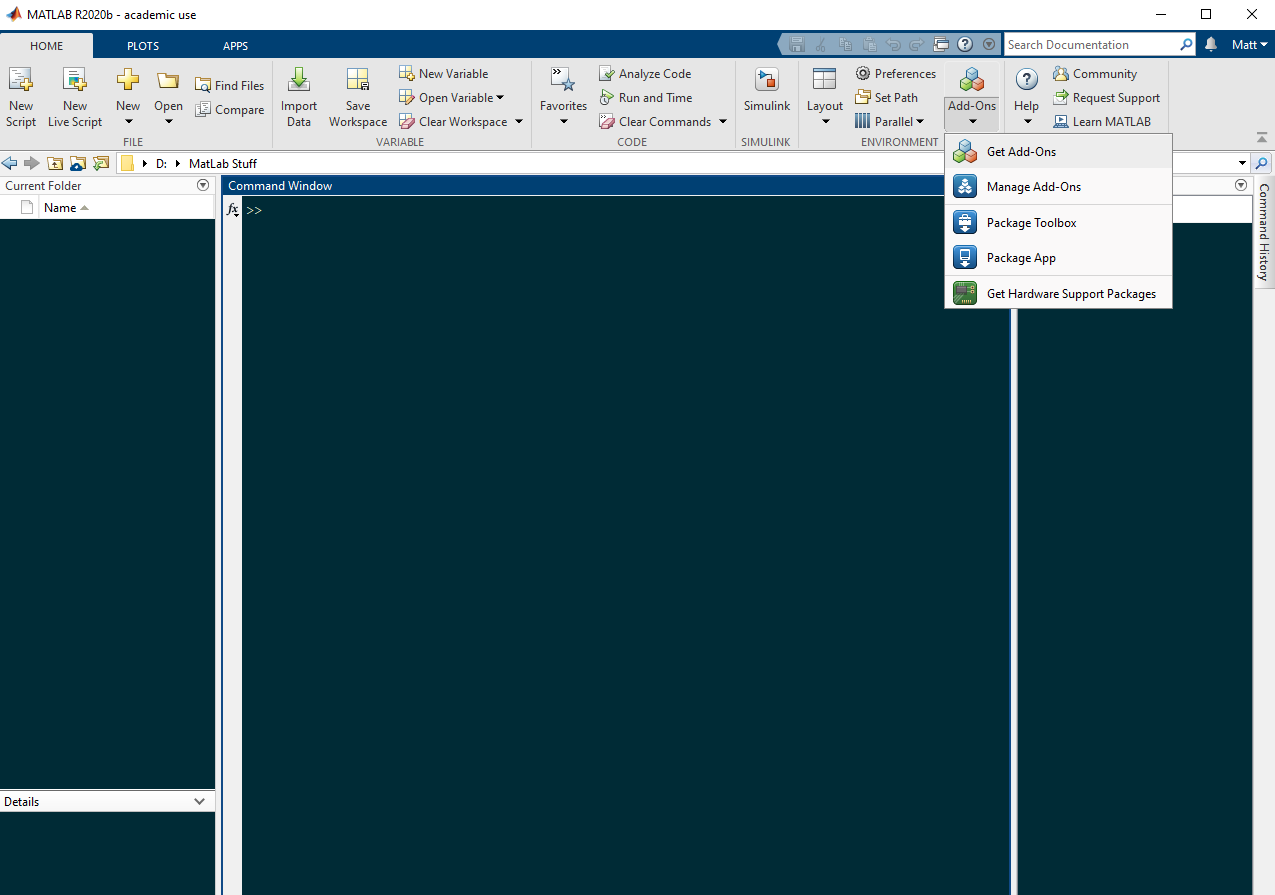
\includegraphics[scale=.45]{matscreen1.png}
          \medskip
\end{minipage}
\item In the Add-On Explorer, search for ‘EntropyHub’.\\
\begin{minipage}[h]{\linewidth}
          \centering
          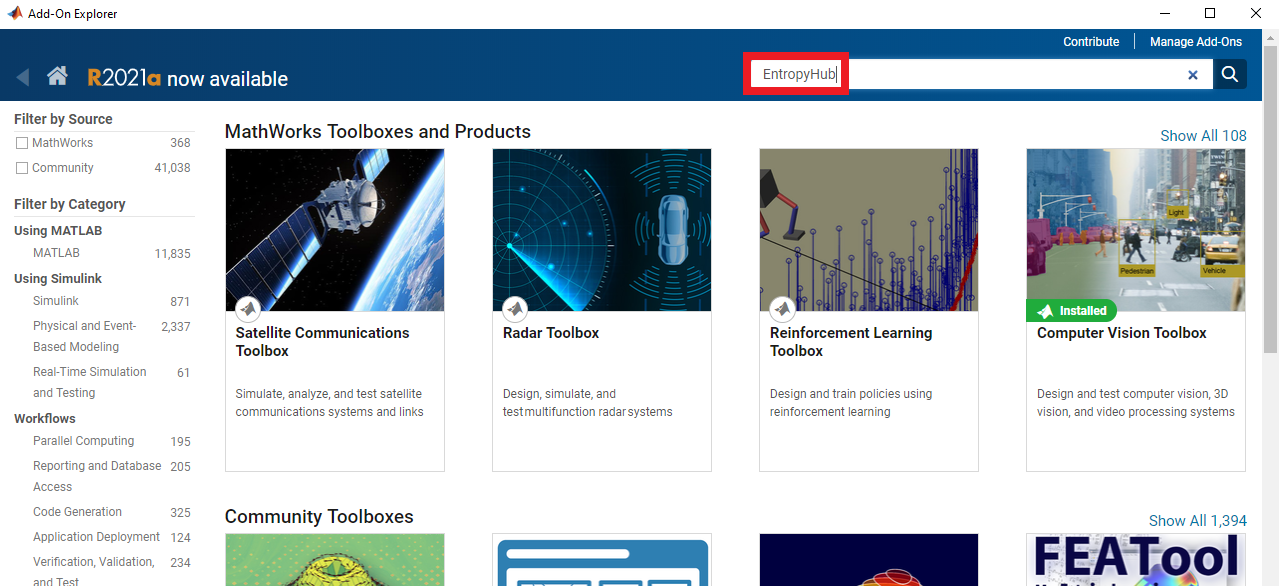
\includegraphics[scale=.45]{matscreen2.png}\\ \ \\
          \medskip
\end{minipage}
\begin{minipage}[h]{\linewidth}
          \centering
          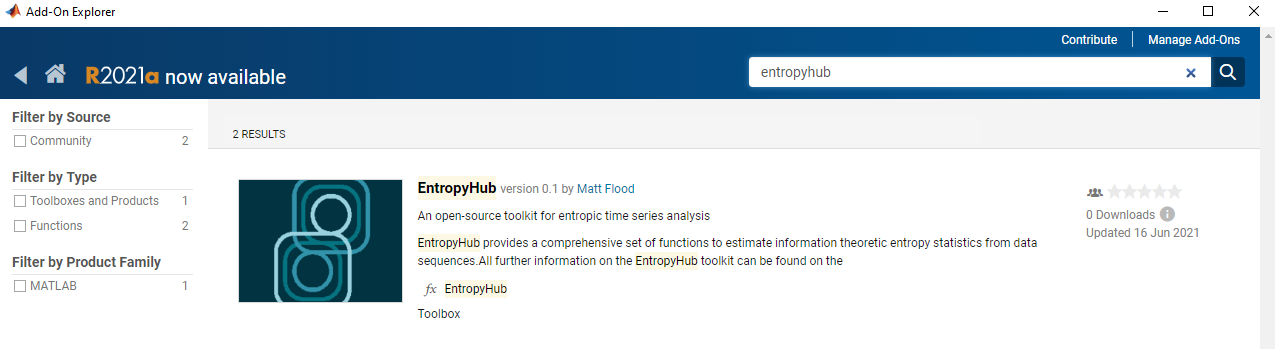
\includegraphics[scale=.45]{matscreen3.png}\\ \ \\
          \medskip
\end{minipage}

\item Open the link to EntropyHub and click the ‘Add’ button in the top right corner.\\ \ \\
\begin{minipage}[h]{\linewidth}
          \centering
          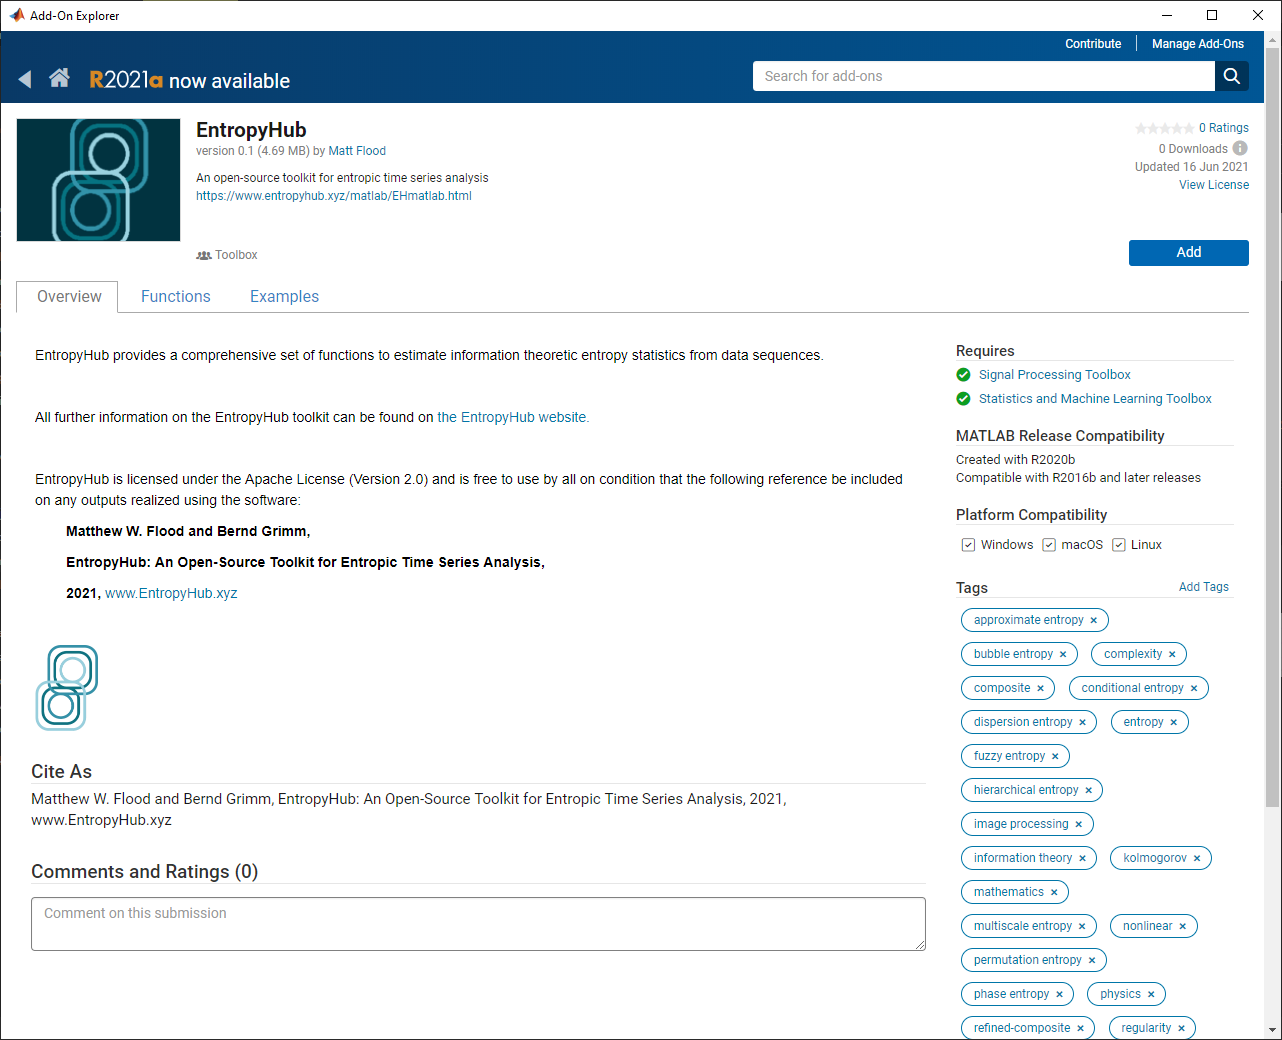
\includegraphics[scale=.35]{matscreen4.png}\\ \ \\
          \medskip
\end{minipage}
\newline
You will be asked to accept the License Agreement prior to installation.\\ \ \\
\begin{minipage}[h]{\linewidth}
          \centering
          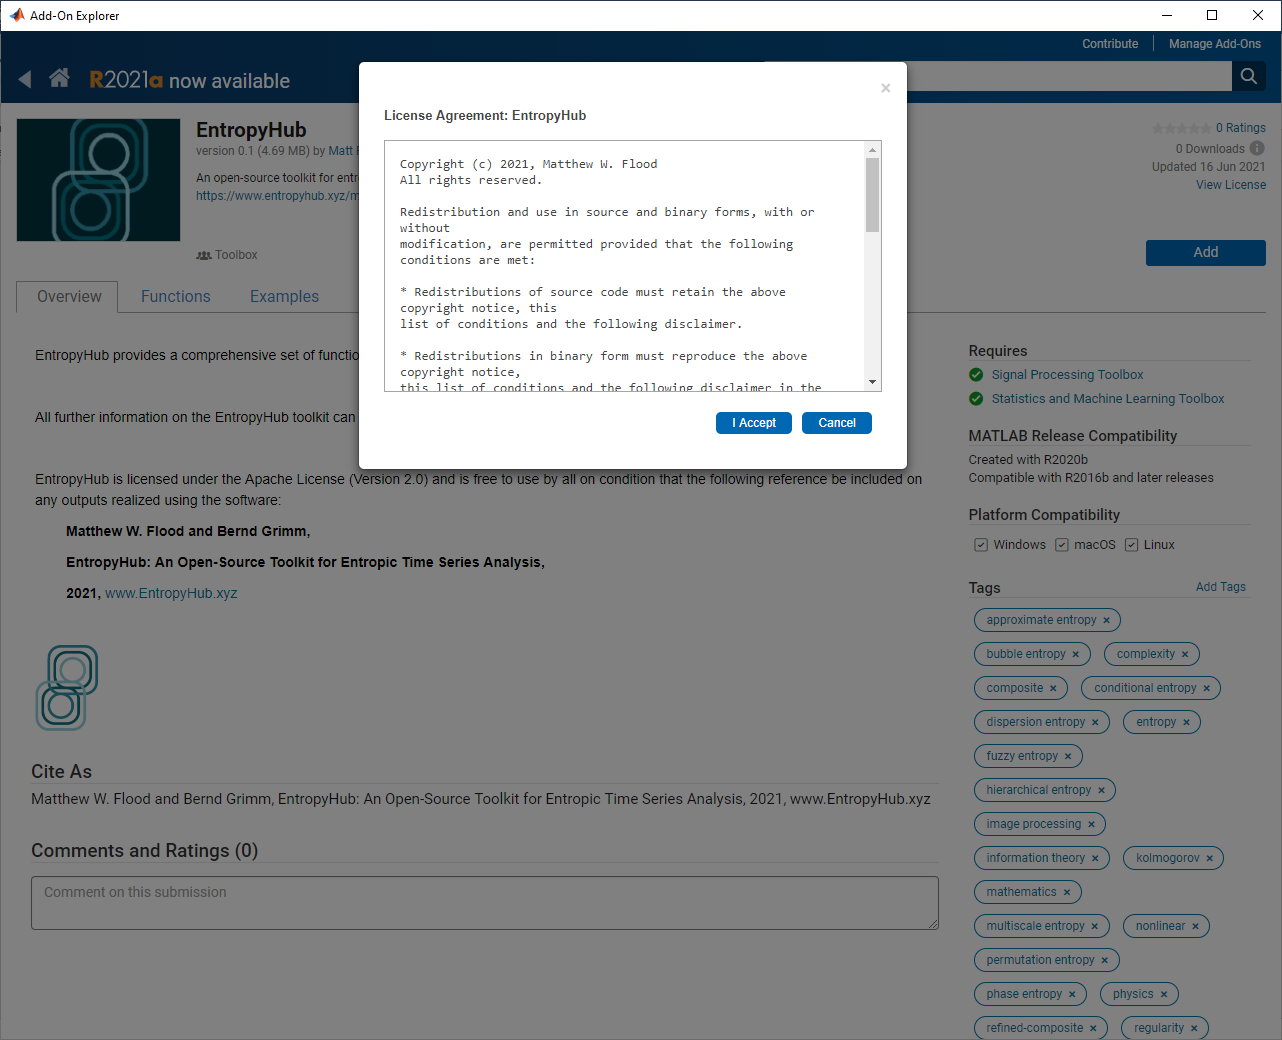
\includegraphics[scale=.35]{matscreen5.png}
          \medskip
\end{minipage}

\end{enumerate}

\subsection*{\normalsize Method 2.}
\begin{enumerate}
\item Visit the \href{https://www.mathworks.com/matlabcentral/fileexchange/94185-entropyhub}{EntropyHub File Exchange page}. \\
Note: you need to be logged in to your MathWorks account to continue.\\
\begin{minipage}[h]{\linewidth}
          \centering
          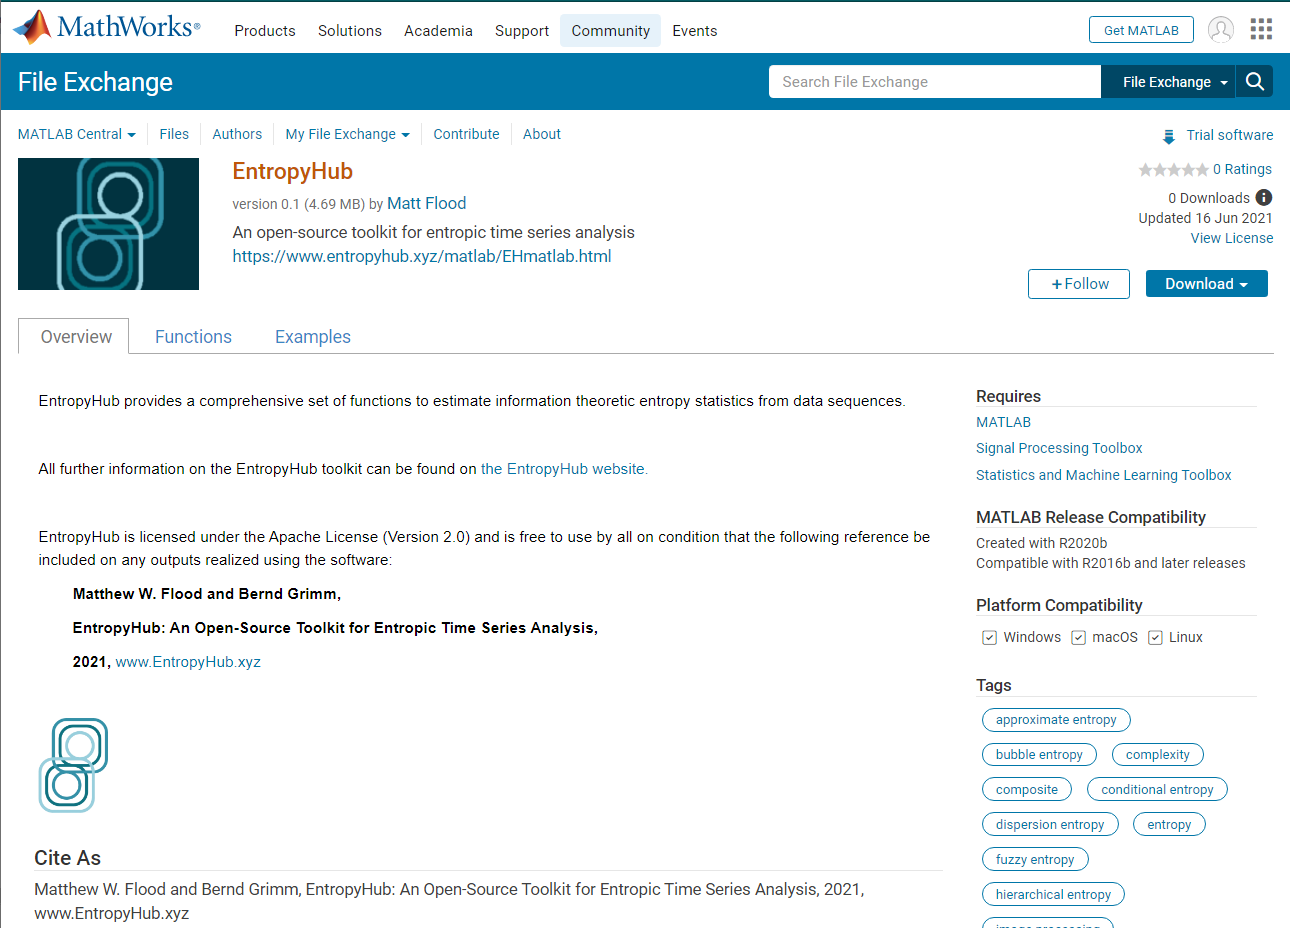
\includegraphics[scale=.35]{matfileexchange.png}\\ \ \\
          \medskip
\end{minipage}
\item Download the toolbox file (EntropyHub.mltbx) by clicking ‘Toolbox’ in the dropdown menu under the ‘Download’ button on the right hand side.
\item	In MatLab, navigate the current folder to the directory where the EntropyHub.mltbx file is saved. Open the file and click install.\\ \ \\
\begin{minipage}[h]{\linewidth}
          \centering
          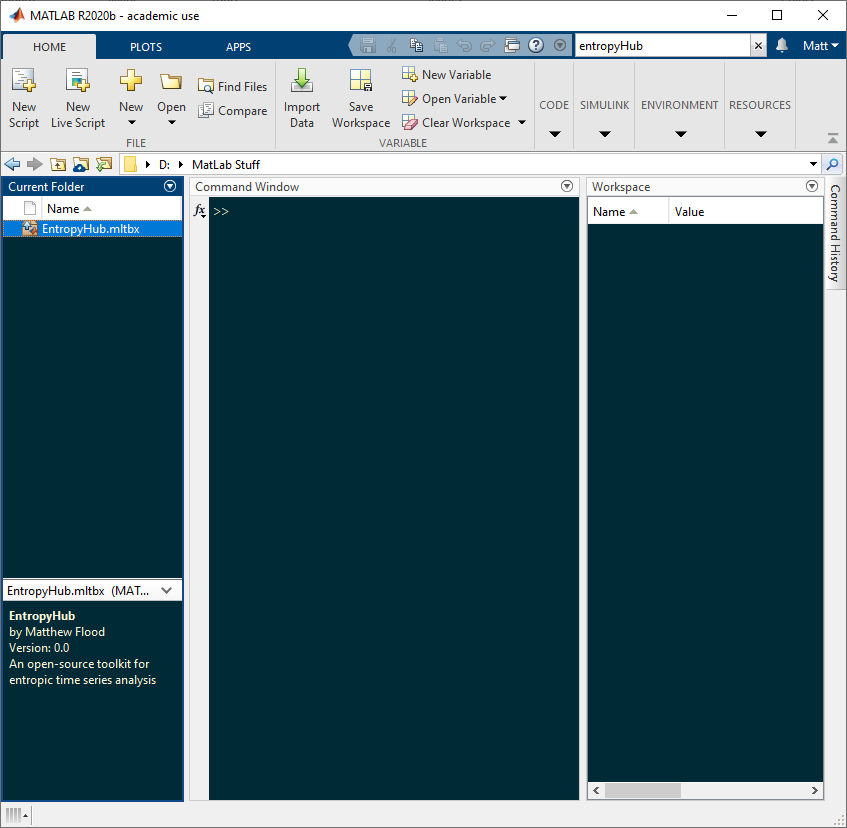
\includegraphics[scale=.6]{MATLAB_README1.png} \\
          \medskip
\end{minipage} 
\begin{minipage}[h]{\linewidth}
          \centering
          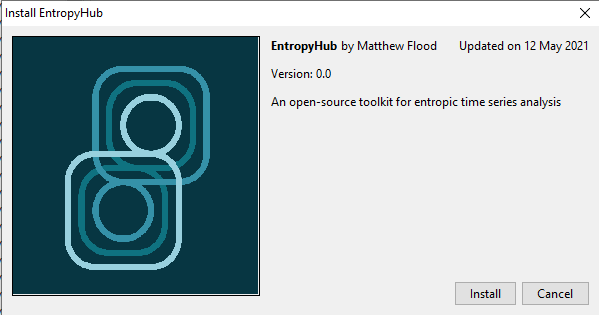
\includegraphics[scale=.7]{MATLAB_README2.png}
          \medskip
\end{minipage}
\end{enumerate}

\subsection*{\normalsize Method 3.}
\begin{enumerate}
\item	Go to the MatLab folder in the \href{https://github.com/MattWillFlood/EntropyHub/tree/main/EntropyHub\%20-\%20MatLab}{EntropyHub  Github repository}.\\ \ \\
\begin{minipage}[h]{\linewidth}
          \centering
          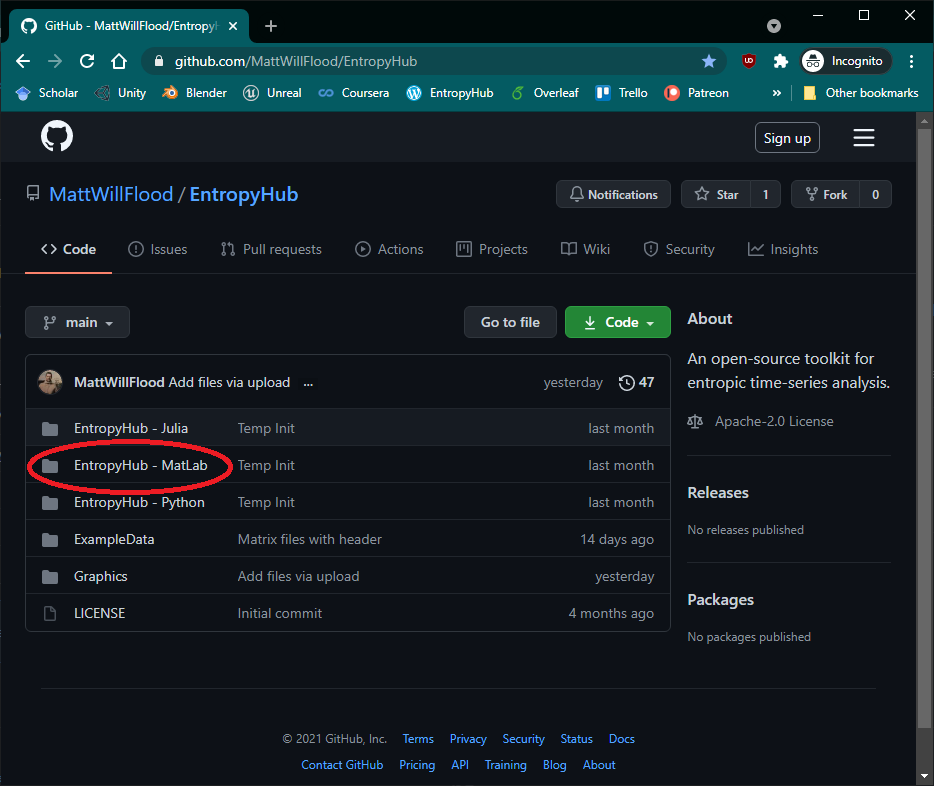
\includegraphics[scale=.6]{MATLAB_README4.png}\\ \ \\
          \medskip
\end{minipage}
\item	Open on the link to the toolbox file (EntropyHub.mltbx) and click the button labelled 'Download'.\\
\begin{minipage}[h]{\linewidth}
          \centering
          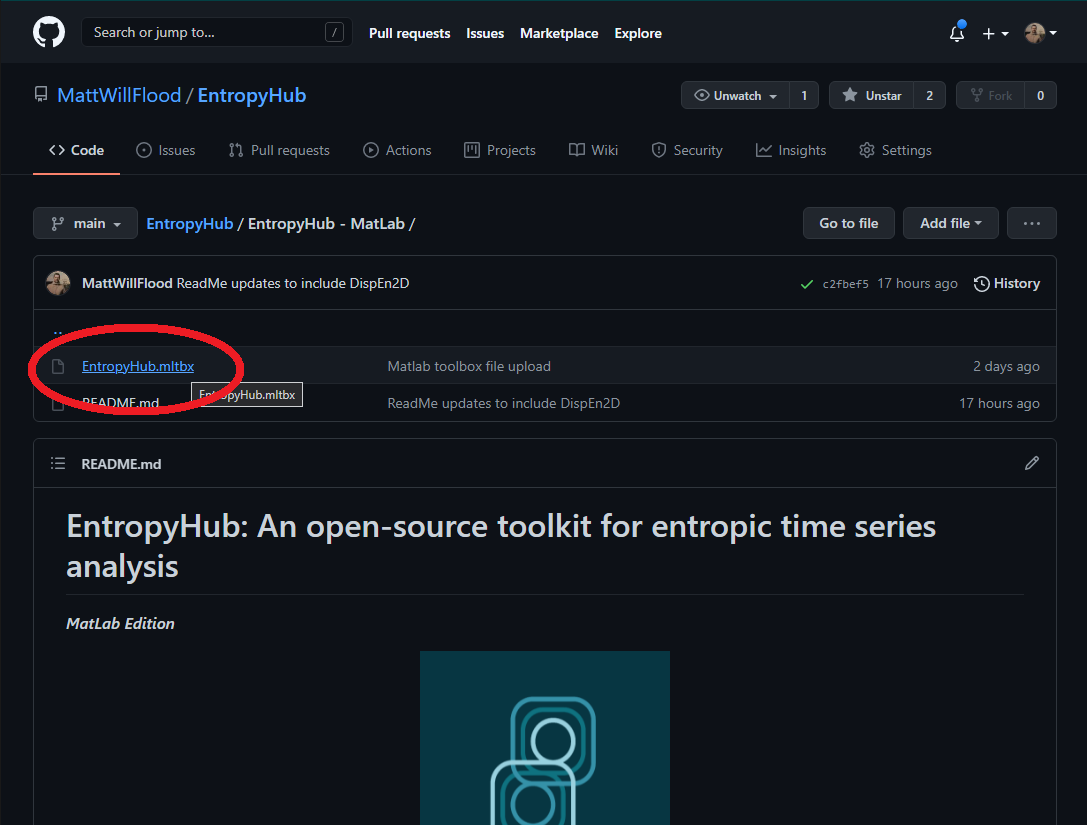
\includegraphics[scale=.5]{matscreen8.png}\\ \ \\	
          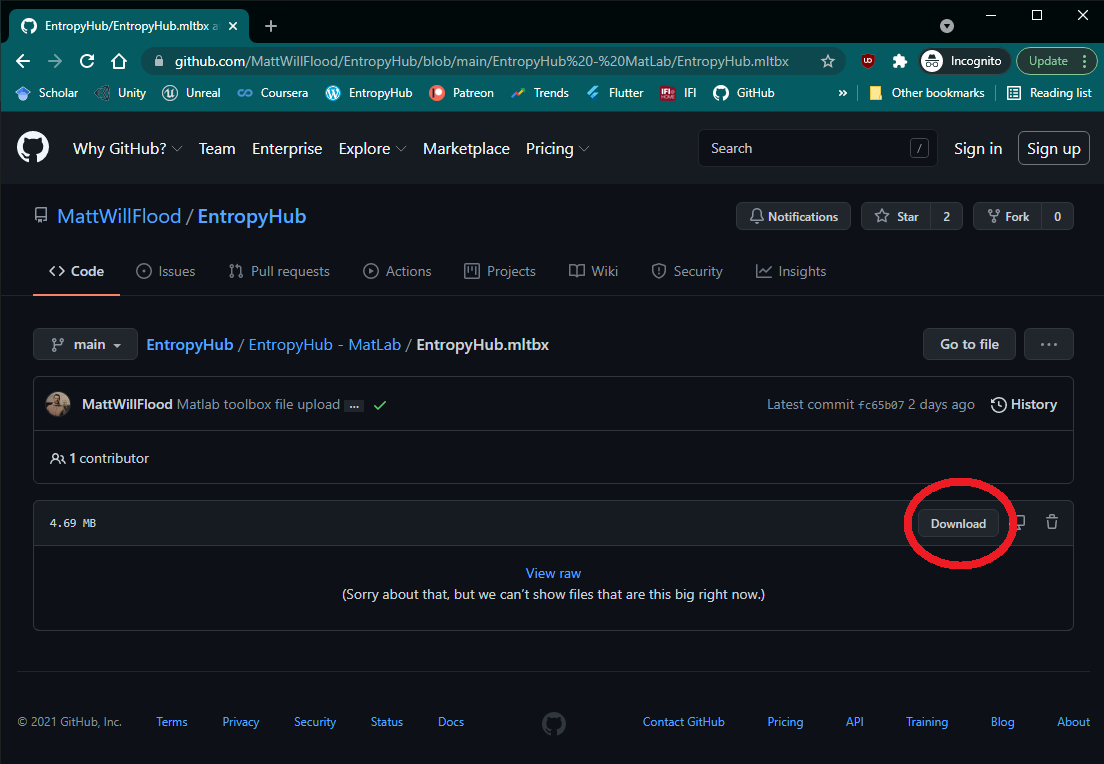
\includegraphics[scale=.5]{matscreen9.png}\\ \ \\
          \medskip
\end{minipage}
\item	In MatLab, navigate the current folder to the directory where the EntropyHub.mltbx file is saved. Open the file and click install.\\
\begin{minipage}[h]{\linewidth}
          \centering
          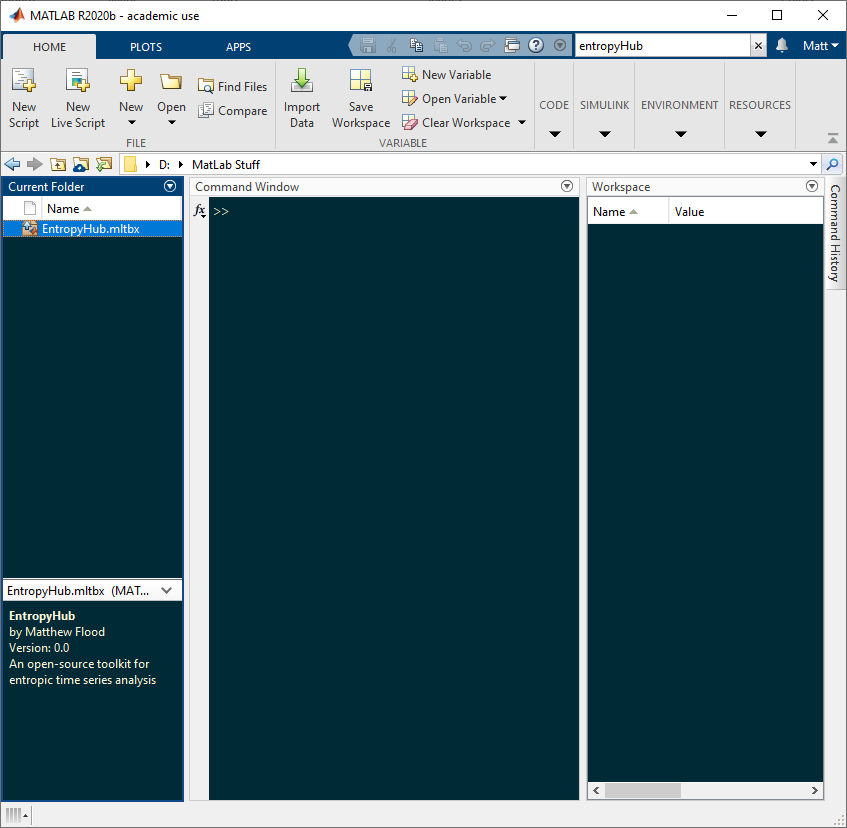
\includegraphics[scale=.6]{MATLAB_README1.png}\\ \ \\
          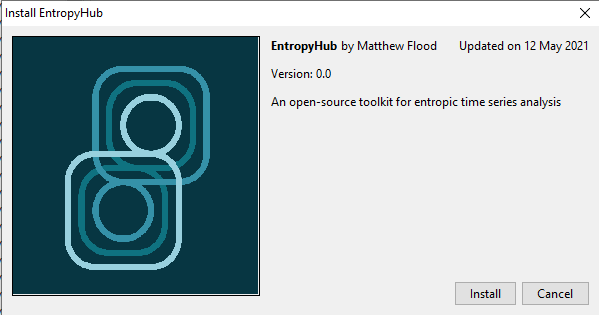
\includegraphics[scale=.7]{MATLAB_README2.png}
          \medskip
\end{minipage}
\end{enumerate}


\newpage
\section{\textbf{Python}}
\subsection*{\normalsize System Requirements}
\noindent There are several package dependencies which will be installed alongside EntropyHub: 

\begin{enumerate}
\item[] \emph{NumPy}
\item[] \emph{SciPy}
\item[] \emph{Matplotlib}
\item[] \emph{PyEMD}
\item[] \emph{Requests}
\end{enumerate}  

\noindent EntropyHub was designed using Python 3 and thus is not intended for use with Python 2. Python versions $>= 3.6$ are required for using EntropyHub.  \\ \ \\ 
\noindent There are 2 ways to install EntropyHub for Python. Method 1 is \textbf{\ul{strongly recommended}}.
\subsection*{\normalsize Method 1.}
\begin{enumerate}	
\item Python comes with an inbuilt package management system, \texttt{pip}. Pip can install, update, or delete any official package. You can install packages via the command line by entering:
\begin{minted}[frame=lines,framesep=2mm,baselinestretch=1.2,bgcolor=ehone]{python}
>>> pip install EntropyHub	
\end{minted}
If using a Python IDE, it is recommended to restart the terminal after installation.

\item To use EntropyHub, import the module with the following command:
\begin{minted}[frame=lines,framesep=2mm,baselinestretch=1.2,bgcolor=ehone]{python}
>>> import EntropyHub
\end{minted}
or in abbreviated form,
\begin{minted}[frame=lines,framesep=2mm,baselinestretch=1.2,bgcolor=ehone]{python}
>>> import EntropyHub as EH
\end{minted}
\end{enumerate}

\subsection*{\normalsize Method 2.}
\noindent \textbf{*Note:} installation with Method 2 requires the latest version of \textbf{\texttt{wheel}} to be previously installed in Python.
\begin{enumerate}
\item	Visit the \href{https://pypi.org/project/EntropyHub/}{EntropyHub PyPI page} 
 (or the \href{https://github.com/MattWillFlood/EntropyHub/tree/main/EntropyHub\%20-\%20Python}{EntropyHub GitHub page}). \\ \ \\
\begin{minipage}[h]{\linewidth}
          \centering
          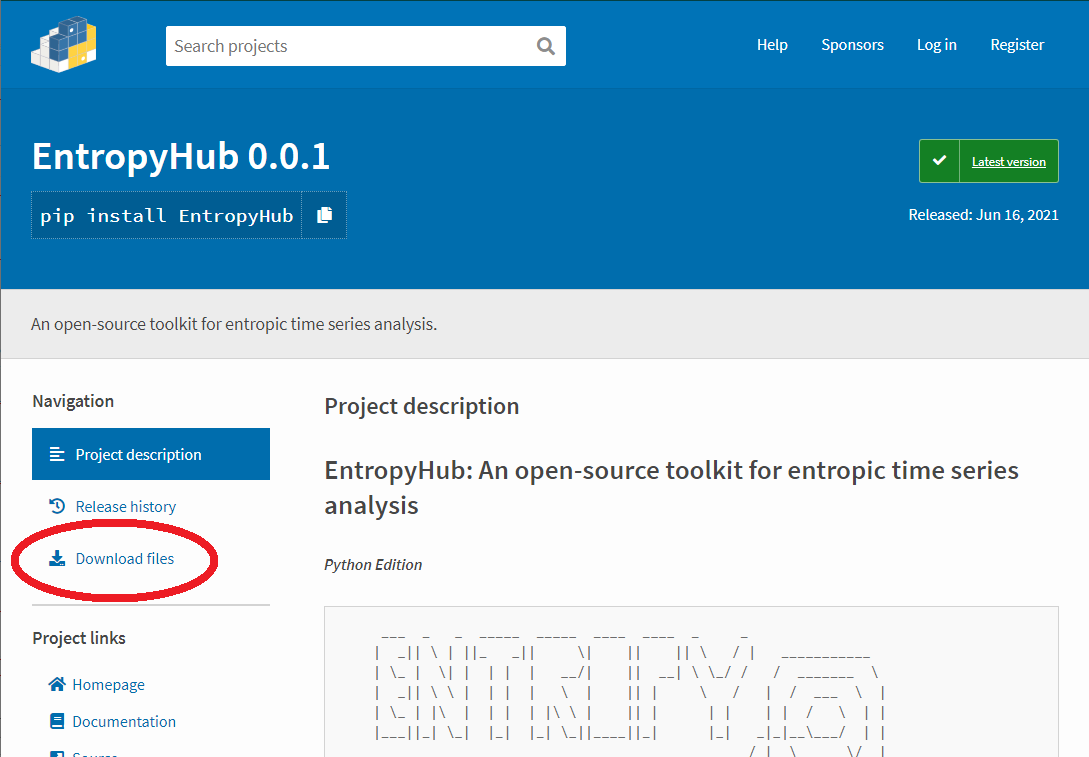
\includegraphics[scale=.5]{pyscreen1.png}
          \medskip
\end{minipage}
 
\item Download the latest .tar.gz folder \textit{(EntropyHub.x.x.x.tar.gz)} from the ‘download files’ button on the left-hand side.\\ \ \\
\begin{minipage}[h]{\linewidth}
          \centering
          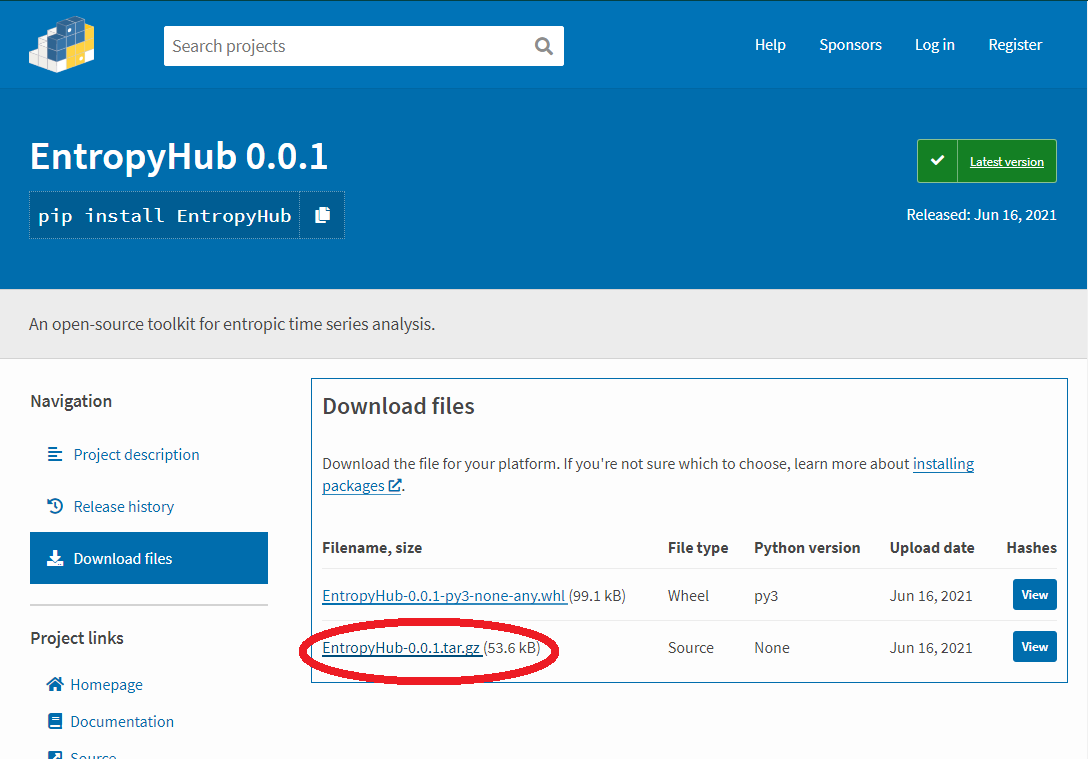
\includegraphics[scale=.5]{pyscreen2.png}
          \medskip
\end{minipage}
\item Extract the files into a local directory.
\item Open a command prompt or terminal window and navigate to the root directory where \textbf{setup.py} is located.

\item In the command line, enter:
\begin{minted}[frame=lines,framesep=2mm,baselinestretch=1.2,bgcolor=ehone]{python}
>>> python setup.py install
\end{minted}
*Ensure that an up-to-date version of \texttt{setuptools} is installed:
\begin{minted}[frame=lines,framesep=2mm,baselinestretch=1.2,bgcolor=ehone]{python}
>>> python -m pip install --upgrade setuptools
\end{minted}
\item To use EntropyHub, import the module with the following command:
\begin{minted}[frame=lines,framesep=2mm,baselinestretch=1.2,bgcolor=ehone]{python}
>>> import EntropyHub
\end{minted}
or in abbreviated form,
\begin{minted}[frame=lines,framesep=2mm,baselinestretch=1.2,bgcolor=ehone]{python}
>>> import EntropyHub as EH
\end{minted}
\end{enumerate}

\newpage
\section{\textbf{Julia}}
\noindent There are several package dependencies which will be installed alongside EntropyHub: 
\begin{enumerate}
\item[] \emph{DataInterpolations.jl}
\item[] \emph{StatsFuns.jl}
\item[] \emph{StatsBase.jl}
\item[] \emph{GroupSlices.jl}
\item[] \emph{Clustering.jl}
\item[] \emph{Combinatorics.jl}
\item[] \emph{DSP.jl}
\item[] \emph{FFTW.jl}
\item[] \emph{HTTP.jl}
\item[] \emph{Statistics.jl}
\item[] \emph{DelimitedFiles.jl}
\item[] \emph{Random.jl}
\item[] \emph{LinearAlgebra.jl}
\item[] \emph{Plots.jl}
\end{enumerate}  

\noindent \ \\
There are 2 ways to install EntropyHub in Julia. Method 1 is recommended.
\subsection*{\normalsize Method 1.}
\begin{enumerate}
\item  In your Julia IDE, open the package REPL and enter:
\begin{minted}[frame=lines,framesep=2mm,baselinestretch=1.2,bgcolor=ehone]{julia}
julia> ]
pkg> add EntropyHub
\end{minted}
or alternatively:
\begin{minted}[frame=lines,framesep=2mm,baselinestretch=1.2,bgcolor=ehone]{julia}
using Pkg
Pkg.add("EntropyHub")
\end{minted}
\item To use EntropyHub in Julia, enter:
\begin{minted}[frame=lines,framesep=2mm,baselinestretch=1.2,bgcolor=ehone]{julia}
using EntropyHub
\end{minted}
or import specific functions:
\begin{minted}[frame=lines,framesep=2mm,baselinestretch=1.2,bgcolor=ehone]{julia}
using EntropyHub: SampEn, MSobject, MSEn
\end{minted}
\end{enumerate}

\subsection*{\normalsize Method 2.}
\begin{enumerate}
\item  Open the Julia package REPL and enter the following:
\begin{minted}[frame=lines,framesep=2mm,baselinestretch=1.2,bgcolor=ehone]{julia}
julia> ]
pkg> add https://github.com/MattWillFlood/EntropyHub.jl
\end{minted}
\item To use EntropyHub in Julia, enter:
\begin{minted}[frame=lines,framesep=2mm,baselinestretch=1.2,bgcolor=ehone]{julia}
using EntropyHub
\end{minted}
or import specific functions:
\begin{minted}[frame=lines,framesep=2mm,baselinestretch=1.2,bgcolor=ehone]{julia}
using EntropyHub: SampEn, MSobject, MSEn
\end{minted}
\end{enumerate}


%------------------------------------------------------------------------
%------------------------------------------------------------------------
\newpage
\chapter{\textbf{Functions}}
\chapterimage[width=16cm, height=3cm]{Chapter Banner2.png}
\vspace{55mm}

Sections 3.1 – 3.8 outline the command line syntax of each function with descriptions of every argument and returned value, as well as references to the source literature. The order of the function commands under the syntax subheading is MatLab first, Python second, Julia third. 

\begin{tcolorbox}[sharp corners, colback=ehone!30, colframe=ehone, title=\textbf{NOTE}]
For concision, function commands written in the following sections using \textbf{Python} syntax exclude the module prefix which would otherwise be required,\\ i.e. \texttt{EntropyHub.SampEn()} is written as \texttt{SampEn()}. 
\end{tcolorbox}

\begin{tcolorbox}[sharp corners, colback=ehone!30, colframe=ehone, title=\textbf{NOTE}]
Python functions in EntropyHub are based primarily on the \texttt{Numpy} module.\\ Arguments in python functions with the \textbf{\texttt{np.}} prefix refer to \texttt{numpy} functions.  
\end{tcolorbox}


\setlength{\parskip}{2em}
%\={4cm}

\newpage
\section{Base Entropy Functions}
\vspace{1cm}
\subsection{\normalsize ApEn: \hspace{15mm} Approximate Entropy} \label{ApEn}
\noindent\ul{Syntax} \vspace{6mm} \\ \noindent \texttt{\footnotesize
[Ap, Phi] = ApEn(Sig, ‘m’, 2, ‘tau’, 1, ‘r’, 0.2*std(Sig), ‘Logx’, exp(1))\\
 Ap, Phi  = ApEn(Sig, m = 2, tau = 1, r = 0.2*np.std(Sig), Logx = np.exp(1))\\
 Ap, Phi  = ApEn(Sig, m = 2, tau = 1, r = 0.2*std(Sig), Logx = exp(1))}

\noindent \ul{Arguments}
\begin{description}[labelsep=1cm, labelwidth=2cm, nosep,,style=multiline,leftmargin=3cm]\footnotesize
\item[\texttt{Sig}]		Time series signal, a vector of length $> 10$.
\item[\texttt{m}]		Embedding dimension, a positive integer.
\item[\texttt{tau}]		Time delay, a positive integer.
\item[\texttt{r}]		Distance threshold, a positive scalar.
\item[\texttt{Logx}]	Logarithm base in the entropy formula, a positive scalar.
\end{description}

\noindent \ul{Outputs}
\begin{description}[labelsep=1cm, labelwidth=2cm, nosep, style=multiline,leftmargin=3cm]\footnotesize
\item[\texttt{Ap}]		Approximate entropy estimates, a vector of length m+1.\\
			**The first value of \texttt{\textbf{Ap}} is the zeroth estimate, i.e. $– \Phi_1$,
				and the last value of \texttt{\textbf{Ap}} is the estimate for the specified \texttt{\textbf{m}}.
\item[\texttt{Phi}]		The number of matched state vectors for each embedding dimension from 0 to m+1.
\end{description}

\noindent \ul{References}\hspace{1cm}
\cite{Ap1}



\newpage
\subsection{\normalsize SampEn: \hspace{15mm} Sample Entropy}\label{SampEn}
\noindent\ul{Syntax} \vspace{6mm} \\ \noindent \texttt{\footnotesize
[Samp, A, B, Vcp\_Ka\_Kb] = SampEn(Sig, ‘m’, 2, ‘tau’, 1, ‘r’, 0.2*std(Sig), ‘Logx’, exp(1), 'Vcp', false) \\
Samp, A, B, Vcp\_Ka\_Kb   = SampEn(Sig, m = 2, tau = 1, r = 0.2*np.std(Sig), Logx = np.exp(1), Vcp = False) \\
Samp, A, B, Vcp\_Ka\_Kb   = SampEn(Sig, m = 2, tau = 1, r = 0.2*std(Sig), Logx = exp(1), Vcp = false)}

\noindent \ul{Arguments}
\begin{description}[labelsep=1cm, labelwidth=2cm, nosep, style=multiline,leftmargin=3cm]\footnotesize
\item[\texttt{Sig}]		Time series signal, a vector of length $> 10$.
\item[\texttt{m}]		Embedding dimension, a positive integer.
\item[\texttt{tau}]		Time delay, a positive integer.
\item[\texttt{r}]		Distance threshold, a positive scalar.
\item[\texttt{Logx}]	Logarithm base in the entropy formula, a positive scalar.
\item[\texttt{Vcp}]		Option to return the variance of the conditional probabilities and the number of overlapping matching vector pairs of lengths \cite{Samp2}

\end{description}

\noindent \ul{Outputs}
\begin{description}[labelsep=1cm, labelwidth=2cm, nosep, style=multiline,leftmargin=3cm]\footnotesize
\item[\texttt{Samp}]		Sample entropy estimates, a vector of length \texttt{\textbf{m+1}}.\\
				**The first value of \texttt{\textbf{Samp}} is the zeroth estimate, i.e. $\frac{1}{2}Log(N(N-1)) – Log(A_1)$, and the last value of \texttt{\textbf{Samp}} is the estimate for the specified \textbf{\texttt{m}}.
\item[\texttt{A}]		The number of matched state vectors for each embedding dimension from 0 to m.
\item[\texttt{B}]		The number of matched state vectors for each embedding dimension from 1 to m+1.
\item[\texttt{Vcp\_Ka\_Kb}]		A vector/tuple of three values corresponding to:
\begin{description}
\item[\texttt{\textbf{Vcp\_Ka\_Kb(1) = V\textsubscript{cp}}}]  Estimate of the variance of conditional probabilities used in the estimation of the sample entropy estimate.
\item[\texttt{\textbf{Vcp\_Ka\_Kb(2) = \textbf{K\textsubscript{a}}}}]  The number of overlapping vector pairs of length m+1
\item[\texttt{\textbf{\textbf{Vcp\_Ka\_Kb(3) = K\textsubscript{b}}}}]  The number of overlapping vector pairs of length m
\end{description}
\ \\ \textbf{**Note:} \texttt{Vcp} is undefined for the zeroth embedding dimension (m = 0) 
 and due to the computational demand, \textbf{\underline{will take substantially more time to return function outputs}}.\\
 See Appendix B in \cite{Samp2} for more info.
\end{description}


\noindent \ul{References}\hspace{1cm}
\cite{Samp1} \cite{Samp2}



\newpage
\subsection{\normalsize FuzzEn: \hspace{15mm}  Fuzzy Entropy} \label{FuzzEn}
\noindent\ul{Syntax} \vspace{6mm} \\ \noindent \texttt{\footnotesize
[Fuzz, Ps1, Ps2] = FuzzEn(Sig, ‘m’, 2, ‘tau’, 1, ‘Fx’, 'default', ‘r’, [0.2, 2], ‘Logx’, exp(1))\\
Fuzz, Ps1, Ps2   = FuzzEn(Sig, m = 2, tau = 1, Fx = "default", r = (0.2, 2), Logx = np.exp(1))\\
Fuzz, Ps1, Ps2   = FuzzEn(Sig, m = 2, tau = 1, Fx = "default", r = (0.2, 2), Logx = exp(1))}

\noindent \ul{Arguments}
\begin{description}[labelsep=1cm, labelwidth=2cm, nosep,style=multiline,leftmargin=3cm]\footnotesize
\item[\texttt{Sig}]		Time series signal, a vector of length $> 10$.
\item[\texttt{m}]		Embedding dimension, a positive integer.
\item[\texttt{tau}]		Time delay, a positive integer.
\item[\texttt{Fx}]		Type of fuzzy function for distance transformation, one of the following strings:
	\begin{description}[labelsep=14em, labelwidth=10em, nosep,style=multiline,leftmargin=6cm]
	\item[\texttt{"default"}]	$f(x) = exp(-\frac{x^{r_2}}{r_1})$\\ \ \\
		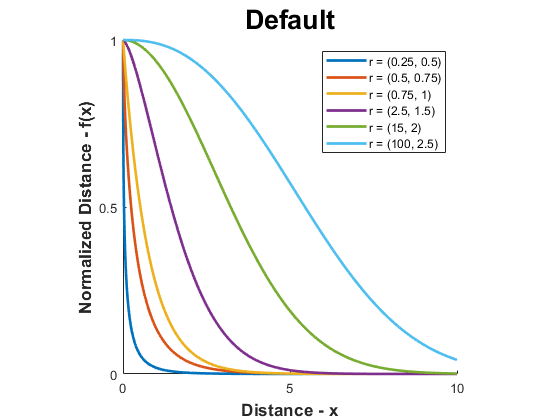
\includegraphics[scale=.5]{Fuzz1v1.png} \\
		 
	\item[\texttt{"sigmoid"/"modsampen"}]	$f(x) = (1+exp(\frac{x-r_2}{r_1}))^{-1}$\\ \ \\
		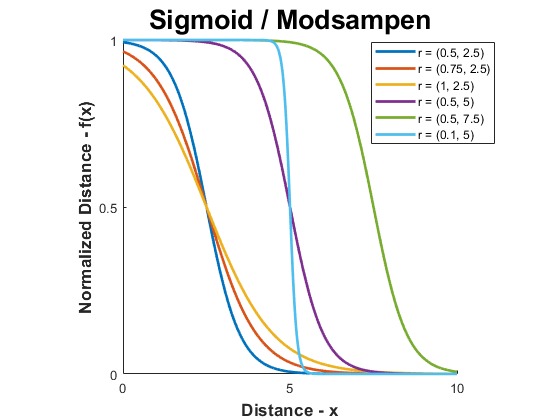
\includegraphics[scale=.5]{Fuzz2v1.png} \\

	\item[\texttt{"triangular"}]	  $f(x) = \begin{cases} 1 - \frac{x}{r},  \hspace{20mm}  x\le r 
	\\ 0,  \hspace{20mm}  x>r \end{cases}$\\
		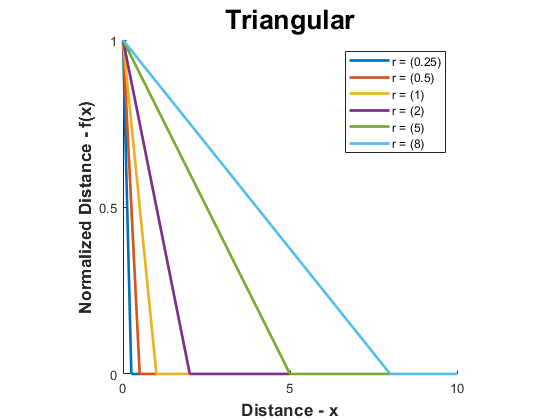
\includegraphics[scale=.5]{FuzzTriv1.png} \\

	\item[\texttt{"trapezoidal1"}]	  $f(x) = \begin{cases} 1,  \hspace{20mm}  x<r 
	\\ 2 - \frac{x}{r},  \hspace{10mm} r\le x<2r 
	\\ 0,  \hspace{20mm}  x\ge 2r \end{cases}$\\
		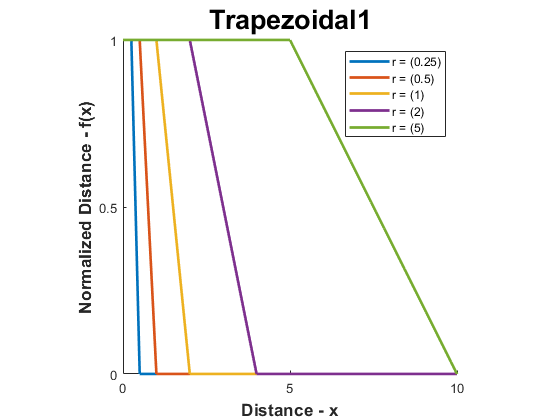
\includegraphics[scale=.5]{FuzzTrap1v1.png} \\ 

	\item[\texttt{"trapezoidal2"}]	  $f(x) = \begin{cases} 1,  \hspace{30mm}  x<r 
	\\ 1 - \frac{x-r_{min}}{r_{max} - r_{min}},  \hspace{5mm} r\le x<r_{max} 
	\\ 0,  \hspace{30mm}  x\ge r_{max} \end{cases}$\\ \ \\
		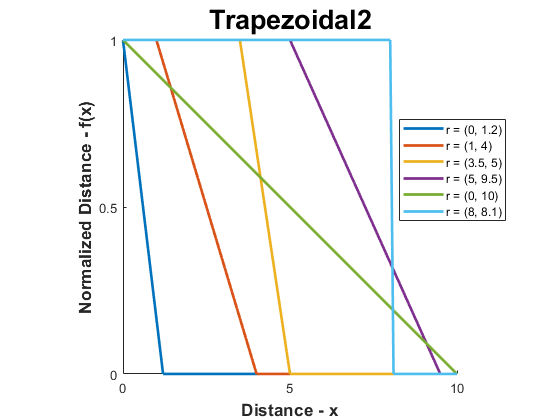
\includegraphics[scale=.5]{FuzzTrap2v1.png} \\ 
		
	\item[\texttt{"z\_shaped"}]	 $f(x) = \begin{cases} 1, \hspace{30mm}  x<r \\ \
	\\ 1 - 2 \left( \frac{x-r}{r}\right)^{2},  \hspace{10mm} r<x<\frac{3}{2}r \\ \
	\\ 2 \left( \frac{x-r}{r}\right)^{2},  \hspace{15mm} \frac{3}{2}r<x<2r \\ \
	\\ 0,  \hspace{30mm}  x>2r \end{cases}$ \\
		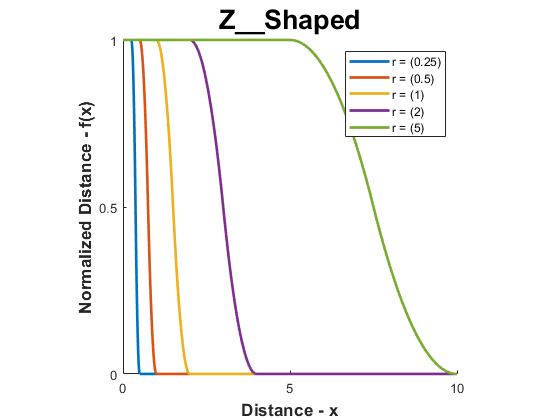
\includegraphics[scale=.5]{FuzzZSv1.png} \\
		
	\item[\texttt{"bell"}] $f\left( x \right) = \frac{1}{1+{\left |\frac{x}{r_1 }\right|}^{r_2 } }$ \\ 
		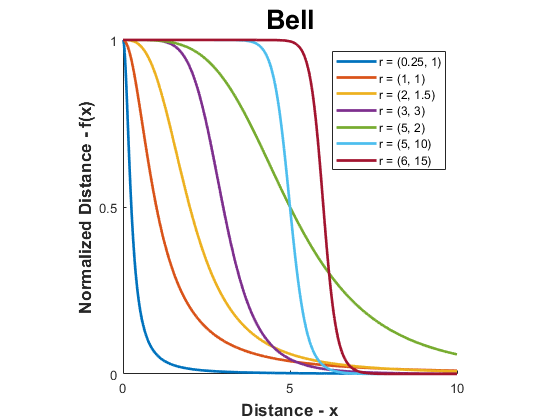
\includegraphics[scale=.5]{FuzzBv1.png}\\
				
	\item[\texttt{"gaussian"}] $f\left( x \right) = exp(-\frac{x^2}{2r^{2}})$ \\ 
		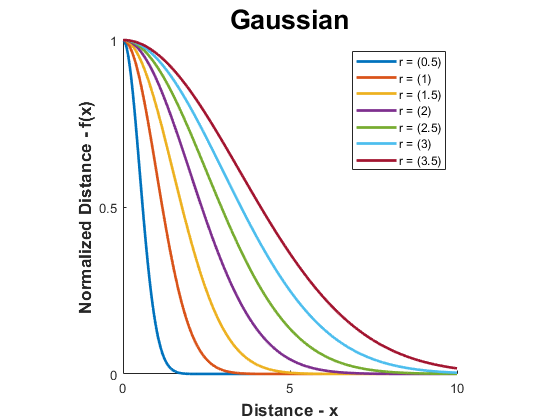
\includegraphics[scale=.5]{FuzzGaussv1.png} \\

	\item[\texttt{"constgaussian"}] $f(x) = \begin{cases} 1,  \hspace{35mm}  x<r_{min} 
	\\  exp(-\log(2)\frac{(x-r)^2}{r}),  \hspace{5mm}  x\ge r_{max} \end{cases}$\\
		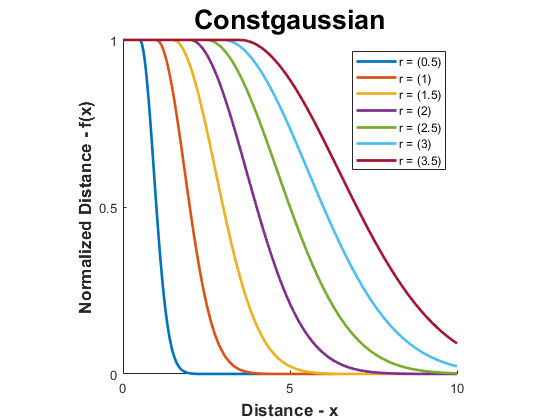
\includegraphics[scale=.5]{FuzzCGv1.png} \\

	\item[\texttt{"gudermannian"}] 	$g(x) = atan(\frac{tanh(r_1)}{x})$
	\item[]	$f(x) = \frac{g(x)}{g(x_{max})}$
	\item[]		Note: Distances are normalized w.r.t. maximum distance relative to each state vector.\\ \ \\
		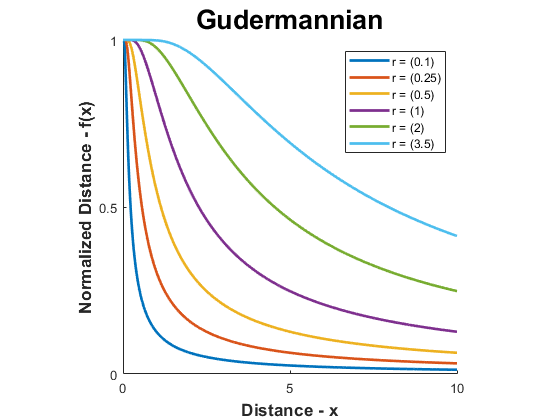
\includegraphics[scale=.5]{FuzzGv1.png} \\
	\end{description}
	
\item[\texttt{r}]	Parameters of the fuzzy function specified by \textbf{\texttt{Fx}}, a 1 element scalar or a 2 element tuple of positive values depending on the fuzzy function as shown above.
	\begin{description}[labelsep=14em, labelwidth=10em, nosep,style=multiline,leftmargin=3cm]
	\item[\texttt{\emph{Default}}]		Two element tuple (or vector in MatLab)
	\item[\texttt{\emph{Sigmoid/ModSampEn}}]		Two element tuple (or vector in MatLab)
	\item[\texttt{\emph{Trapezoidal2}}]		Two element tuple (or vector in MatLab)
	\item[\texttt{\emph{Bell}}]		Two element tuple (or vector in MatLab)
	\item[\texttt{\emph{Trapezoidal1}}]		 A scalar value
	\item[\texttt{\emph{Triangular}}]		 A scalar value
	\item[\texttt{\emph{Z\_Shaped}}]	 A scalar value
	\item[\texttt{\emph{Gaussian}}] A scalar value
	\item[\texttt{\emph{ConstGaussian}}] A scalar value
	\item[\texttt{\emph{Gudermannian}}] A scalar value
	\end{description}

\item[\texttt{Logx}]	Logarithm base in the entropy formula, a positive scalar.
\end{description}

\noindent \ul{Outputs}
\begin{description}[labelsep=1cm, labelwidth=2cm, nosep]\footnotesize
\item[\texttt{Fuzz}]	Fuzzy entropy estimates for each embedding dimension 1:m.
\item[\texttt{Ps1}]		The average fuzzy distances for embedding dimensions 1:m.
\item[\texttt{Ps2}]		The average fuzzy distances for embedding dimensions 2:m+1.
\end{description}

\noindent \ul{References}\hspace{1cm}
\cite{Fuzz1} \cite{Fuzz2} \cite{Fuzz3}



\newpage
\subsection{\normalsize K2En: \hspace{15mm}  Kolmogorov Entropy} \label{K2En}
\noindent\ul{Syntax} \vspace{6mm} \\ \noindent \texttt{\footnotesize
[K2, Ci] = K2En(Sig, ‘m’, 2, ‘tau’, 1, ‘r’, 0.2*std(Sig), ‘Logx’, exp(1)) \\
K2, Ci  = K2En(Sig, m = 2, tau = 1, r = 0.2*np.std(Sig), Logx = np.exp(1)) \\
K2, Ci  = K2En(Sig, m = 2, tau = 1, r = 0.2*std(Sig), Logx = exp(1))}

\noindent \ul{Arguments}
\begin{description}[labelsep=1cm, labelwidth=2cm, nosep, style=multiline,leftmargin=3cm]\footnotesize
\item[\texttt{Sig}]		Time series signal, a vector of length $> 10$.
\item[\texttt{m}]		Embedding dimension, an integer.
\item[\texttt{tau}]		Time delay, a positive integer.
\item[\texttt{r}]		Distance threshold, a positive scalar.
\item[\texttt{Logx}]	Logarithm base in the entropy formula, a positive scalar.
\end{description}

\noindent \ul{Outputs}
\begin{description}[labelsep=1cm, labelwidth=2cm, nosep, style=multiline,leftmargin=3cm]\footnotesize
\item[\texttt{K2}]		Kolmogorov entropy estimates for each embedding dimension from 1 to m
\item[\texttt{Ci}]		The correlation sum for each embedding dimension from 1 to m.
\end{description}

\noindent \ul{References}\hspace{1cm}
\cite{K21} \cite{K22}



\newpage
\subsection{\normalsize PermEn: \hspace{15mm}  Permutation Entropy} \label{PermEn}
\noindent\ul{Syntax} \vspace{6mm} \\ \noindent \texttt{\footnotesize
[Perm, Pnorm, cPE] = PermEn(Sig, ‘m’, 2, ‘tau’, 1, ‘Typex’, ’none’, ‘tpx’, [], ‘Logx’, 2, ‘Norm’, false)\\
Perm, Pnorm, cPE  = PermEn(Sig, m = 2, tau = 1, Typex = ‘none’, tpx = -1, Logx = 2, Norm = False)\\ 
Perm, Pnorm, cPE  = PermEn(Sig, m = 2, tau = 1, Typex = "none", tpx = nothing, Logx = 2, Norm = false) }

\noindent \ul{Arguments}
\begin{description}[labelsep=1cm, labelwidth=2cm, nosep, style=multiline,leftmargin=3cm]\footnotesize
\item[\texttt{Sig}]		Time series signal, a vector of length $> 10$.\\
						It is recommended that length of Sig (N) $>$ 5m! \\  $[Amigo et al., Europhys. Lett. 83:60005, 2008]$
\item[\texttt{m}]		Embedding dimension, an integer $> 1$.
\item[\texttt{tau}]		Time delay, a positive integer.
\item[\texttt{Typex}]	Variant of permutation entropy, one of the following strings:
	\begin{description}[labelsep=10em, labelwidth=6em, nosep,style=multiline,leftmargin=3cm]
		\item[\texttt{"finegrain"}] Fine-grained permutation entropy \cite{Perm2}		
		\item[\texttt{"modified"}] 	Modified permutation entropy \cite{Perm3}
		\item[\texttt{"weighted"}]	Weighted permutation entropy \cite{Perm4}
		\item[\texttt{"ampaware"}]	Amplitude-aware permutation entropy \cite{Perm5}
		\item[\texttt{"edge"}]		Edge permutation entropy  \cite{Perm6}
		\item[\texttt{"uniquant"}]	Uniform quantization-based permutation entropy \cite{Perm7}
		\item[\texttt{"phase"}]  Phase permutation entropy \cite{Perm9}
	\end{description}
\item[\texttt{tpx}]		Tuning parameter for the permutation entropy specified by the  \textbf{\texttt{Typex}} argument.
	\begin{description}[labelsep=10em, labelwidth=4em, nosep,style=multiline,leftmargin=3cm]
	\item[\texttt{\emph{finegrain}}] \textbf{\texttt{tpx}} is the $\alpha$ parameter, a positive scalar (default: 1)	
	\item[\texttt{\emph{ampaware}}]	\textbf{\texttt{tpx}} is the A parameter, a value in range [0 1]  (default: 0.5)
	\item[\texttt{\emph{edge}}]	\textbf{\texttt{tpx}} is the r sensitivity parameter, a scalar $> 0$ (default: 1)
	\item[\texttt{\emph{uniquant}}]	\textbf{\texttt{tpx}} is the L parameter, an integer $> 1$  (default: 4).	
	\item[\texttt{\emph{phase}}]	\textbf{\texttt{tpx}} is the option to unwrap the phase shift of the Hilbert-transformed data sequence, either [\ ] or 1 (default: [\ ]).				
	\end{description}
\item[\texttt{Logx}]	Logarithm base in the entropy formula, a positive scalar.
\item[\texttt{Norm}]    Normalisation of \texttt{\textbf{Pnorm}} value, a boolean operator:\\
					\texttt{false} \hspace{10pt} normalises w.r.t $Log$($\#$ of permutation symbols [m]) - default\\
     		  		\texttt{true} \hspace{15pt} normalises w.r.t $Log$($\#$ of all possible permutations [m!])\\
     		  			* Note: Normalised permutation entropy is undefined for \texttt{m = 1}.\\
     		  			** Note: When \texttt{Typex = uniquant} and \texttt{Norm = true},\\ 									normalisation of \texttt{Perm} is calculated w.r.t. $Log(tpx^m)$
\end{description}

\noindent \ul{Outputs}
\begin{description}[labelsep=1cm, labelwidth=2cm, nosep, style=multiline,leftmargin=3cm]\footnotesize
\item[\texttt{Perm}]	Permutation entropy estimates for embedding dimensions 1:m.
\item[\texttt{Pnorm}]	Normalised Permutation entropy estimates.
\item[\texttt{cPE}]		Conditional permutation entropy \cite{Perm8}
\end{description}

\noindent \ul{References}\hspace{1cm}
\cite{Perm1} \cite{Perm2} \cite{Perm3} \cite{Perm4} \cite{Perm5} \cite{Perm6} \cite{Perm7} \cite{Perm8} \cite{Perm9}



\newpage
\subsection{\normalsize CondEn: \hspace{15mm} \textit{corrected} Conditional Entropy} \label{CondEn}
\noindent\ul{Syntax} \vspace{6mm} \\ \noindent \texttt{\footnotesize
[Cond, SEw, SEz] = CondEn(Sig, ‘m’, 2, ‘tau’, 1, ‘c’, 6, ‘Logx’, exp(1), ‘Norm’, false)\\
 Cond, SEw, SEz  = CondEn(Sig, m = 2, tau = 1, c = 6, Logx = np.exp(1), Norm = False) \\
Cond, SEw, SEz  = CondEn(Sig, m = 2, tau = 1, c = 6, Logx = exp(1), Norm = false)}

\noindent \ul{Arguments}
\begin{description}[labelsep=1cm, labelwidth=2cm, nosep, style=multiline,leftmargin=3cm]\footnotesize
\item[\texttt{Sig}]		Time series signal, a vector of length $> 10$.
\item[\texttt{m}]		Embedding dimension, an integer $> 1$.
\item[\texttt{tau}]		Time delay, a positive integer.
\item[\texttt{c}]		Number of symbols in symbolic transformation, in integer $> 1$
\item[\texttt{Logx}]	Logarithm base in the entropy formula, a positive scalar.
\item[\texttt{Norm}]	Normalization of \texttt{\textbf{Cond}} value:\\
		  \texttt{true} \hspace{15pt}  no normalisation (default)\\
		  \texttt{false} \hspace{10pt}  normalises w.r.t Shannon entropy of data sequence \texttt{\textbf{Sig}}
\end{description}

\noindent \ul{Outputs}
\begin{description}[labelsep=1cm, labelwidth=2cm, nosep, style=multiline,leftmargin=3cm]\footnotesize
\item[\texttt{Cond}]		Corrected conditional entropy estimate
\item[\texttt{SEw}]		Shannon entropy estimate for \texttt{\textbf{m}}.
\item[\texttt{SEz}]		Shannon entropy estimate for \texttt{\textbf{m+1}}.
\end{description}

\noindent \ul{References}\hspace{1cm}
\cite{Cond1}



\newpage
\subsection{\normalsize DistEn: \hspace{15mm} Distribution Entropy} \label{DistEn}
\noindent\ul{Syntax} \vspace{6mm} \\ \noindent \texttt{\footnotesize
[Dist, Ppi] = DistEn(Sig, ‘m’, 2, ‘tau’, 1, ‘Bins’, ‘sturges’, ‘Logx’, 2, ‘Norm’, true)\\
 Dist, Ppi  = DistEn(Sig, m = 2, tau = 1, Bins = ‘sturges’, Logx = 2, Norm = True)\\ 
 Dist, Ppi  = DistEn(Sig, m = 2, tau = 1, Bins = "sturges", Logx = 2, Norm = true)}

\noindent \ul{Arguments}
\begin{description}[labelsep=1cm, labelwidth=2cm, nosep, style=multiline,leftmargin=3cm]\footnotesize
\item[\texttt{Sig}]		Time series signal, a vector of length $> 10$.
\item[\texttt{m}]		Embedding dimension, a positive integer.
\item[\texttt{tau}]		Time delay, a positive integer.
\item[\texttt{Bins}]	Histogram bin selection method, in integer $> 1$ indicating the number of bins, 
						or one of the following strings:\\
   					    "sturges", "sqrt", "rice", "doanes" \hspace{2em} [default: "sturges"]				    
\\ \href{https://en.wikipedia.org/wiki/Histogram#Number_of_bins_and_width}{>> More info on binning methods}.
\item[\texttt{Logx}]	Logarithm base in the entropy formula, a positive scalar.\\
						(Enter 0 for natural logarithm)
\item[\texttt{Norm}]	Normalization of \texttt{\textbf{Dist}} value:\\
		  \texttt{false} \hspace{10pt} no normalisation \\
		  \texttt{true} \hspace{15pt} normalises w.r.t number of histogram bins (default)
\end{description}

\noindent \ul{Outputs}
\begin{description}[labelsep=1cm, labelwidth=2cm, nosep, style=multiline,leftmargin=3cm]\footnotesize
\item[\texttt{Dist}]		Distribution entropy estimate.
\item[\texttt{Phi}]		Probability of each histogram bin.
\end{description}

\noindent \ul{References}\hspace{1cm}
\cite{Dist1}



\newpage
\subsection{\normalsize SpecEn: \hspace{15mm} Spectral Entropy} \label{SpecEn}
\noindent\ul{Syntax} \vspace{6mm} \\ \noindent \texttt{\footnotesize
[Spec, BandEn] = SpecEn(Sig, ‘N’, 2*length(Sig)+1, ‘Freqs’, [0,1], ‘Logx’, exp(1), ‘Norm’, true)\\
 Spec, BandEn  = SpecEn(Sig, N = 2*len(Sig) + 1, Freqs = (0,1), Logx = np.exp(1), Norm = True)\\ 
 Spec, BandEn  = SpecEn(Sig, N = 2*length(Sig) + 1, Freqs = (0,1), Logx = exp(1), Norm = true)}

\noindent \ul{Arguments}
\begin{description}[labelsep=1cm, labelwidth=2cm, nosep, style=multiline,leftmargin=3cm]\footnotesize
\item[\texttt{Sig}]		Time series signal, a vector of length $> 10$.
\item[\texttt{N}]		Resolution of the N-point fft, an integer $> 1$.
\item[\texttt{Freqs}]	Normalised band edge-frequencies for calculating the band entropy (BandEn), a 2 element tuple with values in range [0,1] where 1 is the Nyquist frequency. \\
		* When no edge frequencies are provided, BandEn==SpecEn \\
		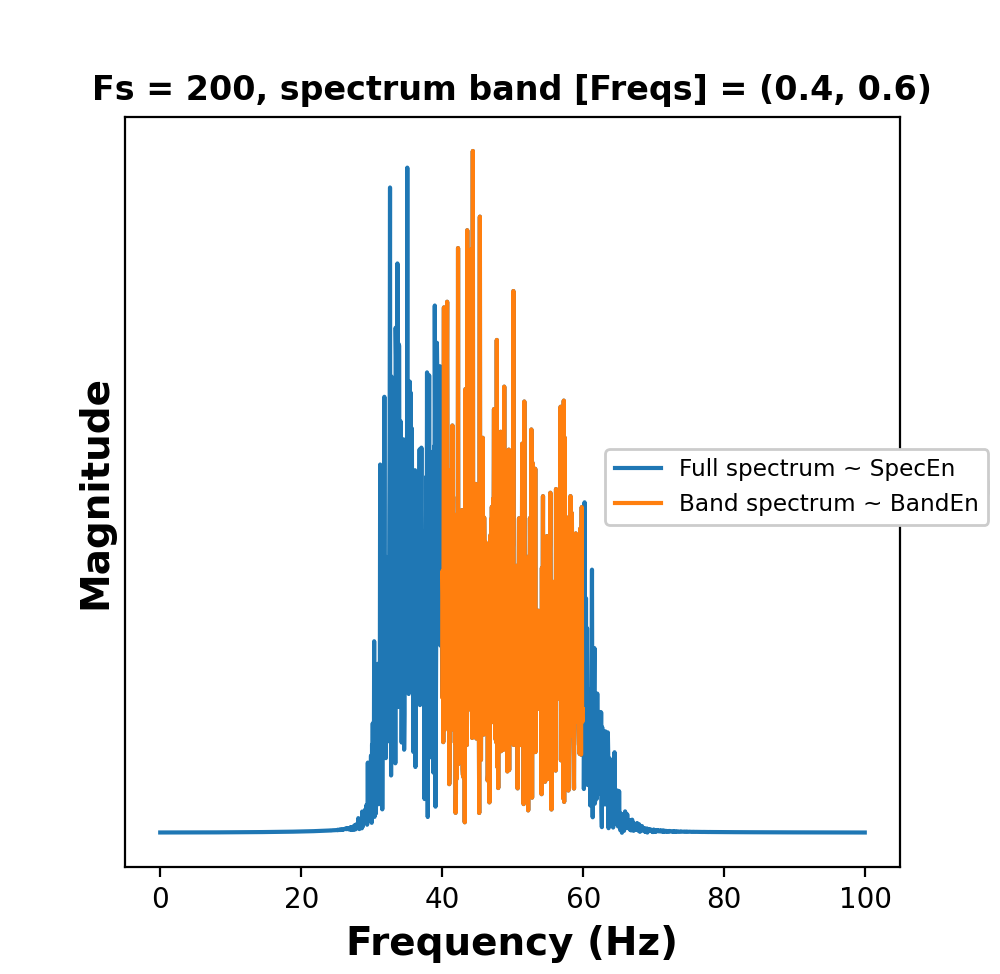
\includegraphics[scale=.55]{Spec1.png}
\item[\texttt{Logx}]	Logarithm base in the entropy formula, a positive scalar.
\item[\texttt{Norm}]	Normalization of \texttt{\textbf{Spec}} value:\\
		  \texttt{false} \hspace{10pt} no normalisation \\
		  \texttt{true} \hspace{15pt}  normalises \texttt{\textbf{Spec}} w.r.t number of Nyquist frequency value, and \texttt{\textbf{BandEn}} w.r.t. range of frequencies in the band given by Freqs. (default)
\end{description}

\noindent \ul{Outputs}
\begin{description}[labelsep=1cm, labelwidth=2cm, nosep, style=multiline,leftmargin=3cm]\footnotesize
\item[\texttt{Spec}]		Spectral entropy estimate.
\item[\texttt{BandEn}]		Spectral band entropy estimate.
\end{description}

\noindent \ul{References}\hspace{1cm}
\cite{Spec1} \cite{Spec2}
\\ \ \\
\noindent\ul{\textbf{Note:}}\hspace{5mm} In contrast to other \textit{Base} entropies, spectral entropy (SpecEn) is not derived from information theory or dynamical systems theory, and instead is an estimate of the frequency spectrum curve estimated using the discrete time Fourier transform.



\newpage
\subsection{\normalsize DispEn: \hspace{15mm} Dispersion Entropy} \label{DispEn}
\noindent\ul{Syntax} \vspace{6mm} \\ \noindent \texttt{\footnotesize
[Dispx, RDE] = DispEn(Sig, ‘m’, 2, ‘tau’, 1, 'c', 3, ‘Typex’, ‘ncdf’, ‘Logx’, exp(1), ‘Fluct’, false, ‘Norm’, false, ‘rho’, 1)\\
 Dispx, RDE  = DispEn(Sig, m = 2, tau = 1, c = 3, Typex = ‘ncdf’, Logx = exp(1), Fluct = False, Norm = False, rho = 1) \\
 Dispx, RDE  = DispEn(Sig, m = 2, tau = 1, c = 3, Typex = "ncdf", Logx = exp(1), Fluct = false, Norm = false, rho = 1)}

\noindent \ul{Arguments}
\begin{description}[labelsep=1cm, labelwidth=2cm, nosep, style=multiline,leftmargin=3cm]\footnotesize
\item[\texttt{Sig}]		Time series signal, a vector of length $> 10$.
\item[\texttt{m}]		Embedding dimension, a positive integer.
\item[\texttt{tau}]		Time delay, a positive integer.
\item[\texttt{c}]		Number of symbols in transform, an integer $> 1$.
\item[\texttt{Typex}]	Type of symbolic sequence transform, one of the following strings:
	\begin{description}[labelsep=5em, labelwidth=8em, nosep,style=multiline,leftmargin=3cm]
		\item[\texttt{"ncdf"}]		Normalised cumulative distribution function  \cite{Disp1}		
		\item[\texttt{"kmeans"}] 	K-means clustering algorithm.\\
		**Note: The \textit{"kmeans"} algorithm uses random initialization conditions.
		 This causes results to vary slightly each time it is called.
		\item[\texttt{"linear"}]	Linear segmentation of signal range 
		\item[\texttt{"finesort"}]	Fine-sorted dispersion entropy \cite{Disp4}
		\item[\texttt{"equal"}]		Approx. equal number of symbols.
		\item[]		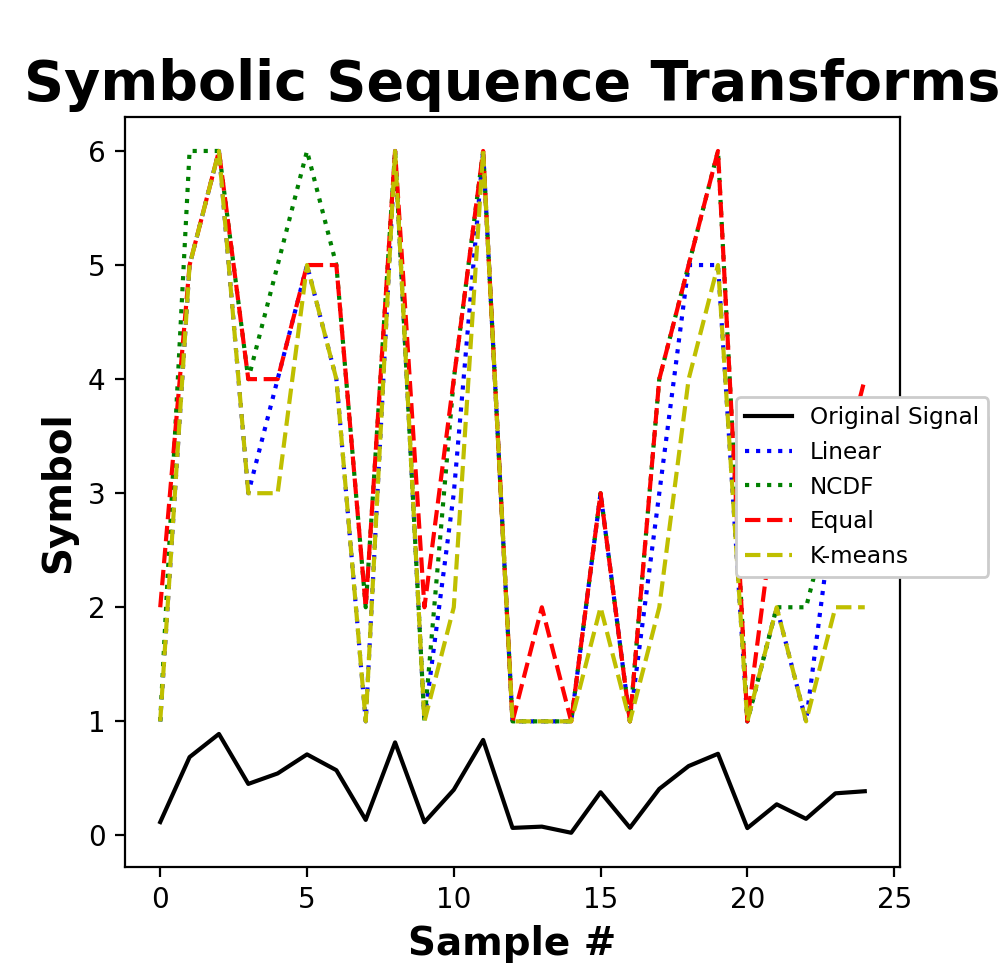
\includegraphics[scale=.75]{Disp1.png}
	\end{description}
\item[\texttt{Logx}]	Logarithm base in the entropy formula, a positive scalar.
\item[\texttt{Fluct}]	When \texttt{\textbf{true}}, returns the fluctuation-based dispersion entropy \cite{Disp2}
\item[\texttt{Norm}]    Normalisation of \texttt{\textbf{Dispx} and \textbf{RDE}} values, a boolean operator:\\
		  \texttt{false} \hspace{10pt} no normalisation \\
		  \texttt{true} \hspace{15pt}  normalises w.r.t number of possible dispersion patterns (default)
\item[\texttt{rho}]		*If \texttt{Typex = "finesort"}, \texttt{\textbf{rho}} is the tuning parameter, a positive scalar (default: 1)
\end{description}

\noindent \ul{Outputs}
\begin{description}[labelsep=1cm, labelwidth=2cm, nosep, style=multiline,leftmargin=3cm]\footnotesize
\item[\texttt{Dispx}]		Dispersion entropy estimate.
\item[\texttt{RDE}]		Reverse dispersion entropy estimate.  \cite{Disp3}
\end{description}

\noindent \ul{References}\hspace{1cm}
\cite{Disp1} \cite{Disp2} \cite{Disp3} \cite{Disp4}



\newpage
\subsection{\normalsize SyDyEn: \hspace{15mm} Symbolic Dynamic Entropy}\label{SyDyEn}
\noindent\ul{Syntax} \vspace{6mm} \\ \noindent \texttt{\footnotesize
[SyDy, Zt] = SyDyEn(Sig, 'm', 2, 'tau', 1, 'c', 3, 'Typex', 'MEP', 'Logx', exp(1), 'Norm', true)\\
SyDy, Zt = SyDyEn(Sig, m = 2, tau = 1, c = 3, Typex = 'MEP', Logx = np.exp(1), Norm = True)\\
SyDy, Zt = SyDyEn(Sig, m = 2, tau = 1, c = 3, Typex = "MEP", Logx = exp(1), Norm = true)}

\noindent \ul{Arguments}
\begin{description}[labelsep=1cm, labelwidth=2cm, nosep, style=multiline,leftmargin=3cm]\footnotesize
\item[\texttt{Sig}]		Time series signal, a vector of length $> 10$.
\item[\texttt{m}]		Embedding dimension, a positive integer.
\item[\texttt{tau}]		Time delay, a positive integer.
\item[\texttt{c}]		Number of symbols, an integer $> 1$.
\item[\texttt{Typex}]	Type of symbolic sequence partitioning, one of the following strings:
	\begin{description}[labelsep=5em, labelwidth=8em, nosep,style=multiline,leftmargin=3cm]
		\item[\texttt{"MEP"}]	Maximum entropy partitioning \cite{SyDy2}		
		\item[\texttt{"kmeans"}] 	K-means clustering algorithm.\\
					*Note: The "kmeans" algorithm uses random initialization conditions.
		 			This causes results to vary slightly when repeatedly called.
		\item[\texttt{"linear"}]	Linear segmentation of signal range 
		\item[\texttt{"uniform"}]	Approx. equal number of symbols.
		\item[ ]				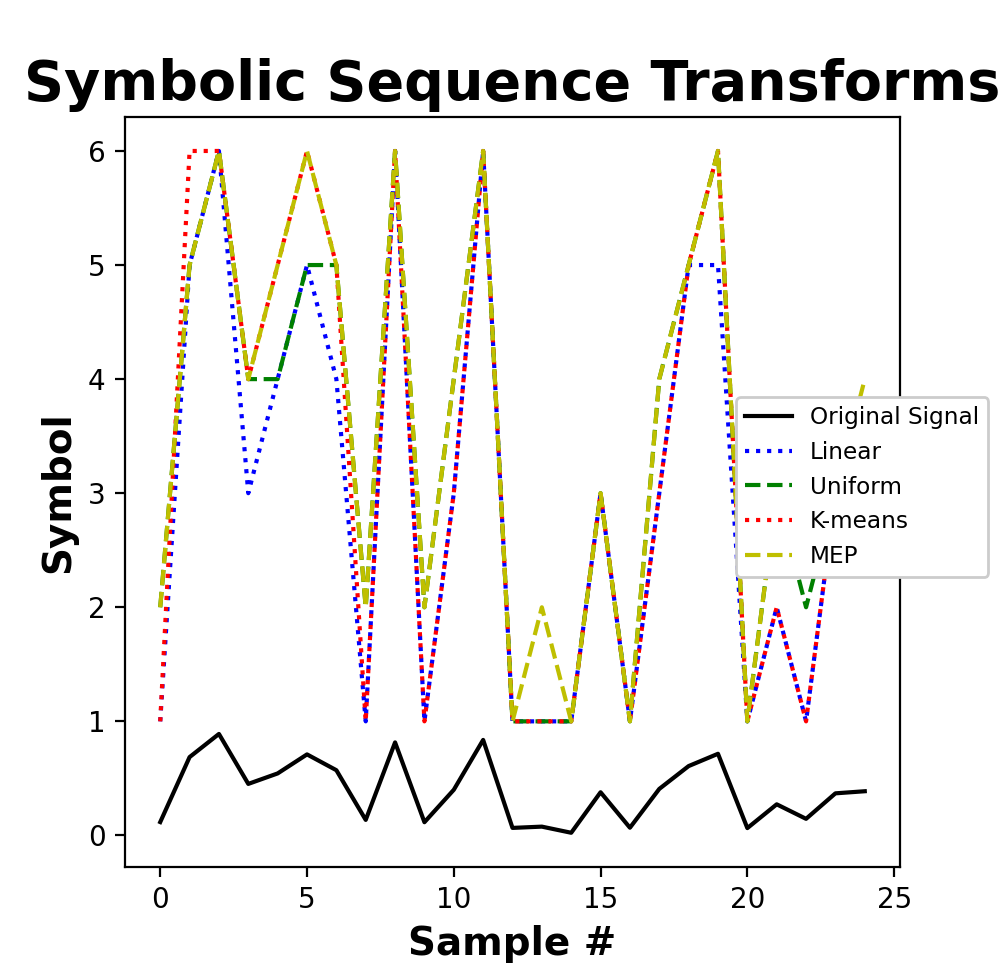
\includegraphics[scale=.75]{SyDy1.png}	\\
		
	\end{description}
\item[\texttt{Logx}]	Logarithm base in the entropy formula, a positive scalar.
\item[\texttt{Norm}]    Normalisation of \texttt{\textbf{SyDy}} value, a boolean operator:\\
		  \texttt{false} \hspace{10pt} no normalisation \\
		  \texttt{true} \hspace{15pt}  normalises w.r.t number of possible vector permutations ($c^{m+1}$) \\
\end{description}

\noindent \ul{Outputs}
\begin{description}[labelsep=1cm, labelwidth=2cm, nosep, style=multiline,leftmargin=3cm]\footnotesize
\item[\texttt{SyDy}]		Symbolic Dynamic entropy estimate.
\item[\texttt{Zt}]		Symbolic sequence of transformed time series.
\end{description}

\noindent \ul{References}\hspace{1cm}
\cite{SyDy1} \cite{SyDy2} \cite{SyDy3}



\newpage
\subsection{\normalsize IncrEn: \hspace{15mm} Increment Entropy}\label{IncrEn}
\noindent\ul{Syntax} \vspace{6mm} \\ \noindent \texttt{\footnotesize
Incr = IncrEn(Sig, ‘m’, 2, ‘tau’, 1, ‘R’, 4, ‘Logx’, exp(1), 'Norm', false) \\
Incr = IncrEn(Sig, m = 2, tau = 1, R = 4, Logx = np.exp(1), Norm = False) \\
Incr = IncrEn(Sig, m = 2, tau = 1, R = 4, Logx = exp(1), Norm = false)}

\noindent \ul{Arguments}
\begin{description}[labelsep=1cm, labelwidth=2cm, nosep, style=multiline,leftmargin=3cm]\footnotesize
\item[\texttt{Sig}]		Time series signal, a vector of length $> 10$.
\item[\texttt{m}]		Embedding dimension, an integer $> 1$.
\item[\texttt{tau}]		Time delay, a positive integer.
\item[\texttt{R}]		Quantifying resolution, a positive scalar.
\item[\texttt{Logx}]	Logarithm base in the entropy formula, a positive scalar.
\item[\texttt{Norm}]	Normalisation of \texttt{\textbf{Incr}} value.\\
						\texttt{false} \hspace{10pt} no normalisation (default)\\
						\texttt{true} \hspace{15pt} normalises w.r.t. embedding dimension (\texttt{\textbf{m-1}})
\end{description}

\noindent \ul{Outputs}
\begin{description}[labelsep=1cm, labelwidth=2cm, nosep, style=multiline,leftmargin=3cm]\footnotesize
\item[\texttt{Incr}]	Increment entropy  estimate.
\end{description}

\noindent \ul{References}\hspace{1cm}
\cite{Incr1} \cite{Incr2} \cite{Incr3}



\newpage
\subsection{\normalsize CoSiEn: \hspace{15mm} Cosine Similarity Entropy}\label{CoSiEn}
\noindent\ul{Syntax} \vspace{6mm} \\ \noindent \texttt{\footnotesize
[CoSi, Bm] = CoSiEn(Sig, ‘m’, 2, ‘tau’, 1, ‘r’, 0.1, ‘Logx’, 2, 'Norm', 0) \\
CoSi, Bm  = CoSiEn(Sig, m = 2, tau = 1, r = 0.1, Logx = 2, Norm = 0) \\
CoSi, Bm  = CoSiEn(Sig, m = 2, tau = 1, r = 0.1, Logx = 2, Norm = 0)}

\noindent \ul{Arguments}
\begin{description}[labelsep=1cm, labelwidth=2cm, nosep, style=multiline,leftmargin=3cm]\footnotesize
\item[\texttt{Sig}]		Time series signal, a vector of length $> 10$.
\item[\texttt{m}]		Embedding dimension, an integer $> 1$.
\item[\texttt{tau}]		Time delay, a positive integer.
\item[\texttt{r}]		Angular threshold, a value in range [0 $<$ \texttt{\textbf{r}} $<$ 1]
\item[\texttt{Logx}]	Logarithm base in the entropy formula, a positive scalar.
\item[\texttt{Norm}]	Normalisation of \texttt{\textbf{Sig}}, an integer in range [0 4]:\\
						0 - no normalisation (default)\\
						1 - median removed\\
						2 - mean removed\\
						3 - normalised to unit variance\\
						4 - normalised to range [-1 1]
\end{description}

\noindent \ul{Outputs}
\begin{description}[labelsep=1cm, labelwidth=2cm, nosep, style=multiline,leftmargin=3cm]\footnotesize
\item[\texttt{CoSi}]	Cosine similarity entropy  estimate.
\item[\texttt{Bm}]	Sum of global probabilities.
\end{description}

\noindent \ul{References}\hspace{1cm}
\cite{CoSi1}



\newpage
\subsection{\normalsize PhasEn: \hspace{15mm} Phase Entropy}\label{PhasEn}
\noindent\ul{Syntax} \vspace{6mm} \\ \noindent \texttt{\footnotesize
Phas = PhasEn(Sig, ‘K’, 4, ‘tau’, 1, ‘Logx’, exp(1), 'Norm', true, 'Plotx', false) \\
Phas = PhasEn(Sig, K = 4, tau = 1, Logx = np.exp(1), Norm = True, Plotx = False) \\
Phas = PhasEn(Sig, K = 4, tau = 1, Logx = exp(1), Norm = true, Plotx = false)}

\noindent \ul{Arguments}
\begin{description}[labelsep=1cm, labelwidth=2cm, nosep, style=multiline,leftmargin=3cm]\footnotesize
\item[\texttt{Sig}]		Time series signal, a vector of length $> 10$.
\item[\texttt{K}]		Number of angular partitions, an integer $>$ 1.\\
				**\textbf{Note:} Angular partitions of the second-order difference plot (SODP) are first split between 0 and \textit{n} degrees w.r.t. the positive x-axis. As this point is somewhat arbitrary, it is recommended to use even-numbered (preferably multiples of 4) partitions for sake of symmetry.
\item[\texttt{tau}]		Time delay, a positive integer.
\item[\texttt{Logx}]	Logarithm base in the entropy formula, a positive scalar.
\item[\texttt{Norm}]	Normalisation of \texttt{\textbf{Phas}}:\\
						\texttt{false} \hspace{10pt} no normalisation (default)\\
						\texttt{true} \hspace{15pt} normalises w.r.t. the number of partitions \texttt{\textbf{Log(K)}}
\item[\texttt{Plotx}]	When \texttt{Plotx == true}, returns SODP (default: \texttt{false})\\
						The example below depicts the SODP of normally distributed random numbers with 7 angular partitions (\texttt{\textbf{K}}).
\item[ ]				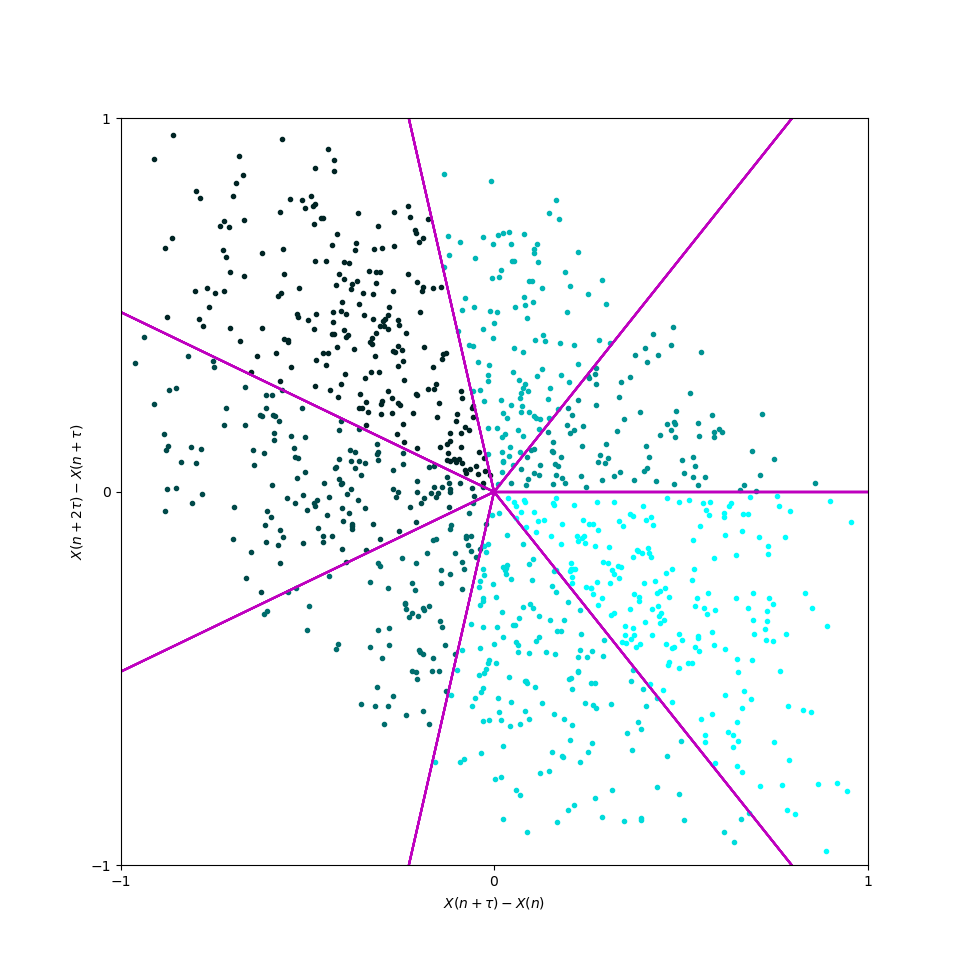
\includegraphics[scale=.34]{Phas1.png}	
\end{description}

\noindent \ul{Outputs}
\begin{description}[labelsep=1cm, labelwidth=2cm, nosep, style=multiline,leftmargin=3cm]\footnotesize
\item[\texttt{Phas}]	Phase entropy estimate.
\end{description}

\noindent \ul{References}\hspace{1cm}
\cite{Phas1}



\newpage
\subsection{\normalsize SlopEn: \hspace{15mm} Slope Entropy}\label{SlopEn}
\noindent\ul{Syntax} \vspace{6mm} \\ \noindent \texttt{\footnotesize
Slop = SlopEn(Sig, ‘m’, 2, ‘tau’, 1, ‘Logx’, 2, 'Lvls', [5, 45], 'Norm', true) \\
Slop = SlopEn(Sig, m = 2, tau = 1, Logx = 2, Lvls = (5, 45), Norm = True) \\
Slop = SlopEn(Sig, m = 2, tau = 1, Logx = 2, Lvls = [5, 45], Norm = true)}

\noindent \ul{Arguments}
\begin{description}[labelsep=1cm, labelwidth=2cm, nosep, style=multiline,leftmargin=3cm]\footnotesize
\item[\texttt{Sig}]		Time series signal, a vector of length $> 10$.
\item[\texttt{m}]		Embedding dimension, an integer $> 1$.
\item[\texttt{tau}]		Time delay, a positive integer.
\item[\texttt{Logx}]	Logarithm base in the entropy formula, a positive scalar.\\
			Enter 0 for natural logarithm.
\item[\texttt{Lvls}]	Angular thresolds, a vector (or tuple in python) of monotonically increasing   
              values in the range [0 90] degrees
\item[\texttt{Norm}]	Normalisation of \texttt{\textbf{Slop}}:\\
						\texttt{false} \hspace{10pt} no normalisation \\
						\texttt{true} \hspace{15pt} normalises w.r.t. the number of unique patterns found.
\end{description}

\noindent \ul{Outputs}
\begin{description}[labelsep=1cm, labelwidth=2cm, nosep, style=multiline,leftmargin=3cm]\footnotesize
\item[\texttt{Slop}]	Slope entropy estimates, a vector of length m-1 where values correspond to embedding dimensions [2, ..., m]
\end{description}

\noindent \ul{References}\hspace{1cm}
\cite{Slop1}



\newpage
\subsection{\normalsize BubbEn: \hspace{15mm} Bubble Entropy}\label{BubbEn}
\noindent\ul{Syntax} \vspace{6mm} \\ \noindent \texttt{\footnotesize
[Bubb, H] = BubbEn(Sig, ‘m’, 2, ‘tau’, 1, ‘Logx’, exp(1)) \\
Bubb, H = BubbEn(Sig, m = 2, tau = 1, Logx = np.exp(1)) \\
Bubb, H = BubbEn(Sig, m = 2, tau = 1, Logx = exp(1))}

\noindent \ul{Arguments}
\begin{description}[labelsep=1cm, labelwidth=2cm, nosep, style=multiline,leftmargin=3cm]\footnotesize
\item[\texttt{Sig}]		Time series signal, a vector of length $> 10$.
\item[\texttt{m}]		Embedding dimension, an integer $ > 1$.
\item[\texttt{tau}]		Time delay, a positive integer.
\item[\texttt{Logx}]	Logarithm base in the entropy formula, a positive scalar.\\
\end{description}

\noindent \ul{Outputs}
\begin{description}[labelsep=1cm, labelwidth=2cm, nosep, style=multiline,leftmargin=3cm]\footnotesize
\item[\texttt{Bubb}]	Bubb entropy estimate.
\item[\texttt{H}]	Conditional Rényi entropy
\end{description}

\noindent \ul{References}\hspace{1cm}
\cite{Bubb1}



\newpage
\subsection{\normalsize GridEn: \hspace{15mm} Gridded Distribution Entropy}\label{GridEn}
\noindent\ul{Syntax} \vspace{6mm} \\ \noindent \texttt{\footnotesize
[GDE, GDR, PIx, GIx, SIx, AIx]  = GridEn(Sig, ‘m’, 3, ‘tau’, 1, ‘Logx’, exp(1), 'Plotx', false) \\
GDE, GDR, PIx, GIx, SIx, AIx = GridEn(Sig, m = 3, tau = 1, Logx = np.exp(1), Plotx = False) \\
GDE, GDR, PIx, GIx, SIx, AIx = GridEn(Sig, m = 3, tau = 1, Logx = exp(1), Plotx = false)}

\noindent \ul{Arguments}
\begin{description}[labelsep=1cm, labelwidth=2cm, nosep, style=multiline,leftmargin=3cm]\footnotesize
\item[\texttt{Sig}]		Time series signal, a vector of length $> 10$.
\item[\texttt{m}]		Number of grid divisions, an integer $ > 1$.
\item[\texttt{tau}]		Time delay, a positive integer.
\item[\texttt{Logx}]	Logarithm base in the entropy formula, a positive scalar.
\item[\texttt{Plotx}]	When \texttt{Plotx == true}, returns Poicaré plot and a bivariate histogram of the grid point distribution (default: \texttt{false})
\item[ ]			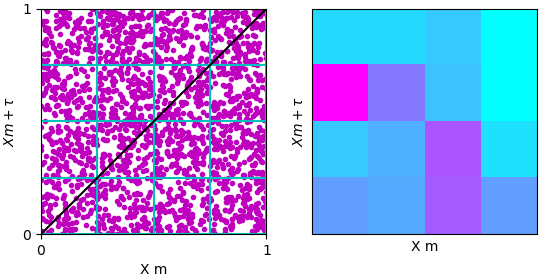
\includegraphics[scale=.5]{Grid1.png}\\
			\textit{Poincaré plot and bivariate histogram of uniform random number sequence (m = 4).\\
					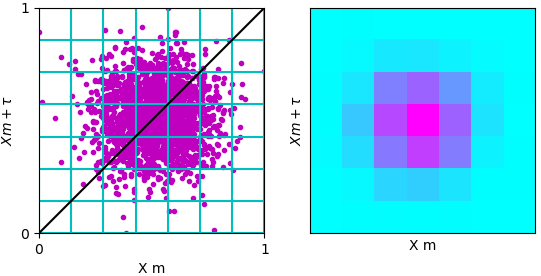
\includegraphics[scale=.5]{Grid2.png}\\
					Poincaré plot and bivariate histogram of white noise (m = 7).}
\end{description}

\noindent \ul{Outputs}
\begin{description}[labelsep=1cm, labelwidth=2cm, nosep, style=multiline,leftmargin=3cm]\footnotesize
\item[\texttt{GDE}]	Gridded distribution entropy estimate.
\item[\texttt{GDR}]	Gridded distribution rate.
\item[\texttt{PIx}]	Percentage of points below the line of identity (LI). \cite{Grid3}
\item[\texttt{GIx}]	Proportion of point distances above the LI. \cite{Grid5}
\item[\texttt{SIx}]	Ratio of phase angles (w.r.t. LI) of the points above the LI.\cite{Grid4} 
\item[\texttt{AIx}]	Ratio of the cumulative area of sectors of points above the LI.\cite{Grid2}
\end{description}

\noindent \ul{References}\hspace{1cm}
\cite{Grid1} \cite{Grid2} \cite{Grid3} \cite{Grid4} \cite{Grid5}



\newpage
\subsection{\normalsize EnofEn: \hspace{15mm} Entropy of Entropy} \label{EnofEn}
\noindent\ul{Syntax} \vspace{6mm} \\ \noindent \texttt{\footnotesize
[EoE, AvEn, S2]  = EnofEn(Sig, ‘tau’, 10, ‘S’, 10, ‘Xrange’, [min(Sig) max(Sig)], ‘Logx’, exp(1)) \\
EoE, AvEn, S2 = EnofEn(Sig, tau = 10, S = 10, Xrange = (np.min(Sig), np.max(Sig)), Logx = np.exp(1)) \\
EoE, AvEn, S2 = EnofEn(Sig, tau = 10, S = 10, Xrange = (min(Sig),max(Sig)), Logx = exp(1)}

\noindent \ul{Arguments}
\begin{description}[labelsep=1cm, labelwidth=2cm, nosep, style=multiline,leftmargin=3cm]\footnotesize
\item[\texttt{Sig}]		Time series signal, a vector of length $> 10$.
\item[\texttt{tau}]		Window length, an integer $> 1$ and $<$ length(Sig)
\item[\texttt{S}]		Number of slices (s1), an integer $> 1$
\item[\texttt{Xrange}]	The min and max of the range included in the division of slices, \\
						a two-element tuple where Xrange[0] $<=$ Xrange[1]
\item[\texttt{Logx}]	Logarithm base in the entropy formula, a positive scalar.
\end{description}

\noindent \ul{Outputs}
\begin{description}[labelsep=1cm, labelwidth=2cm, nosep, style=multiline,leftmargin=3cm]\footnotesize
\item[\texttt{EoE}]	Entropy of entropy estimate.
\item[\texttt{AvEn}]	Average Shannon entropy across all windows.
\item[\texttt{S2}]	Number of levels (S2) used for the given tau and S.
\end{description}

\noindent \ul{References}\hspace{1cm}
\cite{EoE1}



\newpage
\subsection{\normalsize AttnEn: \hspace{15mm} Attention Entropy} \label{AttnEn}
\noindent\ul{Syntax} \vspace{6mm} \\ \noindent \texttt{\footnotesize
[Attn, Hxx, Hnn, Hxn, Hnx]  = EnofEn(Sig, ‘Logx’, 2) \\
Attn, Hxx, Hnn, Hxn, Hnx = EnofEn(Sig, Logx = 2) \\
Attn, Hxx, Hnn, Hxn, Hnx = EnofEn(Sig, Logx = 2)}

\noindent \ul{Arguments}
\begin{description}[labelsep=1cm, labelwidth=2cm, nosep, style=multiline,leftmargin=3cm]\footnotesize
\item[\texttt{Sig}]		Time series signal, a vector of length $> 10$.
\item[\texttt{Logx}]	Logarithm base in the entropy formula, a positive scalar.\\
		Enter 0 for natural logarithm.
\end{description}

\noindent \ul{Outputs}
\begin{description}[labelsep=1cm, labelwidth=2cm, nosep, style=multiline,leftmargin=3cm]\footnotesize
\item[\texttt{Attn}]	Attention entropy estimate.
\item[\texttt{Hxx}]	    Entropy of local-maxima intervals
\item[\texttt{Hnn}]	    Entropy of local-minima intervals
\item[\texttt{Hxn}]	    Entropy of intervals between local maxima and subsequent minima
\item[\texttt{Hnx}]	    Entropy of intervals between local minima and subsequent maxima  
\end{description}

\noindent \ul{References}\hspace{1cm}
\cite{Attn1}



\newpage
\subsection{\normalsize DivEn: \hspace{15mm} Diversity Entropy} \label{DivEn}
\noindent\ul{Syntax} \vspace{6mm} \\ \noindent \texttt{\footnotesize
[Div, CDEn, Bm] = DivEn(Sig, 'm', 2, 'tau', 1, 'r', 5, 'Logx', exp(1)) \\
Div, CDEn, Bm = DivEn(Sig, m = 2, tau = 1, r = 5, Logx = np.exp(1)) \\
Div, CDEn, Bm = DivEn(Sig, m = 2, tau = 1, r = 5, Logx = exp(1))}

\noindent \ul{Arguments}
\begin{description}[labelsep=1cm, labelwidth=2cm, nosep, style=multiline,leftmargin=3cm]\footnotesize
\item[\texttt{Sig}]		Time series signal, a vector of length $> 10$.
\item[\texttt{m}]		Embedding dimension, an integer $ > 1$.
\item[\texttt{tau}]		Time delay, a positive integer.
\item[\texttt{r}]		Histogram bins, either: \\- an integer  $>1$ representing the number of bins \\- a vector array of 3 or more increasing values in range [-1 1] representing the bin edges including the rightmost edge.
\item[\texttt{Logx}]	Logarithm base in the entropy formula, a positive scalar.\\
		Enter 0 for natural logarithm.
\end{description}

\noindent \ul{Outputs}
\begin{description}[labelsep=1cm, labelwidth=2cm, nosep, style=multiline,leftmargin=3cm]\footnotesize
\item[\texttt{Div}]	Diversity entropy estimate.
\item[\texttt{CDEn}]	Cumulative diversity entropy estimate.
\item[\texttt{Bm}]	    Probability from each histogram bin.
\end{description}

\noindent \ul{References}\hspace{1cm}
\cite{Div1} \cite{Div2}



\newpage
\subsection{\normalsize RangEn: \hspace{15mm} Range Entropy} \label{RangEn}
\noindent\ul{Syntax} \vspace{6mm} \\ \noindent \texttt{\footnotesize
[Rangx, A, B] = RangEn(Sig, 'm', 2, 'tau', 1, 'r', 0.2, 'Methodx', 'SampEn', 'Logx', exp(1)) \\
Rangx, A, B = RangEn(Sig, m = 2, tau = 1, r = 0.2, Methodx = "SampEn", Logx = np.exp(1)) \\
Rangx, A, B = RangEn(Sig, m = 2, tau = 1, r = 0.2, Methodx = "SampEn", Logx = exp(1))}


\noindent \ul{Arguments}
\begin{description}[labelsep=1cm, labelwidth=2cm, nosep, style=multiline,leftmargin=3cm]\footnotesize
\item[\texttt{Sig}]		Time series signal, a vector of length $> 10$.
\item[\texttt{m}]		Embedding dimension, an integer $ > 1$.
\item[\texttt{tau}]		Time delay, a positive integer.
\item[\texttt{r}]		Distance threshold, a positive scalar
\item[\texttt{Methodx}]		Method for entropy estimation, either "ApEn" or "SampEn"  
\item[\texttt{Logx}]	Logarithm base in the entropy formula, a positive scalar.\\
		Enter 0 for natural logarithm.
\end{description}

\noindent \ul{Outputs}
\begin{description}[labelsep=1cm, labelwidth=2cm, nosep, style=multiline,leftmargin=3cm]\footnotesize
\item[\texttt{Rangx}]	Range entropy estimate.
\item[\texttt{A}]	Number of matched state vectors of length m+1.
\item[\texttt{B}]	Number of matched state vectors of length m.
\end{description}

\noindent \ul{References}\hspace{1cm}
\cite{Rang1} \cite{Ap1} \cite{Samp1}





%------------------------------------------------------------------------
%------------------------------------------------------------------------
\newpage
\section{Cross-Entropy Functions}
\vspace{1cm}

\subsection{\normalsize XApEn: \hspace{15mm} Cross-Approximate Entropy}\label{XApEn}
\noindent\ul{Syntax} \vspace{6mm} \\ \noindent \texttt{\footnotesize
[XAp, Phi] = XApEn(Sig1, Sig2, ‘m’, 2, ‘tau’, 1, ‘r’, 0.2*std\textsubscript{pooled}(Sig1, Sig2), ‘Logx’, exp(1))\\
 XAp, Phi  = XApEn(Sig1, Sig2, m = 2, tau = 1, r = 0.2*std\textsubscript{pooled}(Sig1, Sig2), Logx = np.exp(1))\\
 XAp, Phi  = XApEn(Sig1, Sig2, m = 2, tau = 1, r = 0.2*std\textsubscript{pooled}(Sig1, Sig2), Logx = exp(1))}

\noindent \ul{Arguments}
\begin{description}[labelsep=1cm, labelwidth=2cm, nosep,,style=multiline,leftmargin=3cm]\footnotesize
\item[\texttt{Sig1}]	First data sequence, a vector of $>10$ elements.
\item[\texttt{Sig2}]	Second data sequence, a vector of $>10$ elements.\\
\textbf{NOTE: \ul{XApEn is direction-dependent}}. Thus, \texttt{\textbf{Sig1}} is used as the template data sequence, and the \texttt{\textbf{Sig2}} is the matching sequence.
\item[\texttt{m}]		Embedding dimension, a positive integer.
\item[\texttt{tau}]		Time delay, a positive integer.
\item[\texttt{r}]		Distance threshold, a positive scalar.
\item[\texttt{Logx}]	Logarithm base in the entropy formula, a positive scalar.
\end{description}

\noindent \ul{Outputs}
\begin{description}[labelsep=1cm, labelwidth=2cm, nosep, style=multiline,leftmargin=3cm]\footnotesize
\item[\texttt{XAp}]		Cross-approximate entropy estimates, a vector of length m+1.\\
		**The first value of \texttt{\textbf{XAp}} is the zeroth estimate, i.e. $– \Phi_1$, and the last value of \texttt{\textbf{XAp}} is the estimate for the specified \texttt{\textbf{m}}.
\item[\texttt{Phi}]		The number of matched state vectors for each embedding dimension from 0 to m+1.
\end{description}

\noindent \ul{References}\hspace{1cm}
\cite{Ap1}



\newpage
\subsection{\normalsize XSampEn: \hspace{15mm} Cross-Sample Entropy}\label{XSampEn}
\noindent\ul{Syntax} \vspace{6mm} \\ \noindent \texttt{\footnotesize
[XSamp, A, B, Vcp\_Ka\_Kb] = XSampEn(Sig1, Sig2, ‘m’, 2, ‘tau’, 1, ‘r’, 0.2*std\textsubscript{pooled}(Sig1, Sig2), ‘Logx’, exp(1), 'Vcp', false)\\
 XSamp, A, B, Vcp\_Ka\_Kb  = XSampEn(Sig1, Sig2, m = 2, tau = 1, r = 0.2*std\textsubscript{pooled}(Sig1, Sig2), Logx = np.exp(1), Vcp = False)\\
 XSamp, A, B, Vcp\_Ka\_Kb  = XSampEn(Sig1, Sig2, m = 2, tau = 1, r = 0.2*std\textsubscript{pooled}(Sig1, Sig2), Logx = exp(1), Vcp = false)}

\noindent \ul{Arguments}
\begin{description}[labelsep=1cm, labelwidth=2cm, nosep,,style=multiline,leftmargin=3cm]\footnotesize
\item[\texttt{Sig1}]	First data sequence, a vector of $>10$ elements.
\item[\texttt{Sig2}]	Second data sequence, a vector of $>10$ elements.
\item[\texttt{m}]		Embedding dimension, a positive integer.
\item[\texttt{tau}]		Time delay, a positive integer.
\item[\texttt{r}]		Radius distance threshold, a positive scalar.
\item[\texttt{Logx}]	Logarithm base in the entropy formula, a positive scalar.
\item[\texttt{Vcp}]		Option to return the variance of the conditional probabilities and the number of overlapping matching vector pairs of lengths
\end{description}

\noindent \ul{Outputs}
\begin{description}[labelsep=1cm, labelwidth=2cm, nosep, style=multiline,leftmargin=3cm]\footnotesize
\item[\texttt{XSamp}]		Cross-sample entropy estimates, a vector of length m+1.\\
			**The first value of \texttt{\textbf{XSamp}} is the zeroth estimate, i.e.  $Log(N1*N2) \ – \ Log(A_1)$,
			and the last value of \texttt{\textbf{XSamp}} is the estimate for the specified \texttt{\textbf{m}}.
\item[\texttt{A}]		The number of matched state vectors for each embedding dimension from 0 to m.
\item[\texttt{B}]		The number of matched state vectors for each embedding dimension from 1 to m+1.
\item[\texttt{Vcp\_Ka\_Kb}]		A vector/tuple of three values corresponding to:
\begin{description}
\item[\texttt{\textbf{Vcp\_Ka\_Kb(1) = V\textsubscript{cp}}}]  Estimate of the variance of conditional probabilities used in the estimation of the sample entropy estimate.
\item[\texttt{\textbf{Vcp\_Ka\_Kb(2) = \textbf{K\textsubscript{a}}}}]  The number of overlapping vector pairs of length m+1
\item[\texttt{\textbf{\textbf{Vcp\_Ka\_Kb(3) = K\textsubscript{b}}}}]  The number of overlapping vector pairs of length m
\end{description}
\ \\ \textbf{**Note:} \texttt{Vcp} is undefined for the zeroth embedding dimension (m = 0) 
 and due to the computational demand, \textbf{\underline{will take substantially more time to return function outputs}}.\\
 See Appendix B in \cite{Samp2} for more info.
\end{description}

\noindent \ul{References}\hspace{1cm}
\cite{Samp1} \cite{Samp2}



\newpage
\subsection{\normalsize XFuzzEn: \hspace{15mm} Cross-Fuzzy Entropy} \label{XFuzzEn}
\noindent\ul{Syntax} \vspace{6mm} \\ \noindent \texttt{\footnotesize
[XFuzz, Ps1, Ps2] = XFuzzEn(Sig1, Sig2, ‘m’, 2, ‘tau’, 1, ‘Fx’, ‘default, ‘r’, [0.2, 2], ‘Logx’, exp(1))\\
XFuzz, Ps1, Ps2   = XFuzzEn(Sig1, Sig2, m = 2, tau = 1, Fx = 'default', r = (0.2, 2), Logx = np.exp(1))\\
XFuzz, Ps1, Ps2   = XFuzzEn(Sig1, Sig2, m = 2, tau = 1, Fx = "default", r = (0.2, 2), Logx = exp(1))}

\noindent \ul{Arguments}
\begin{description}[labelsep=1cm, labelwidth=2cm, nosep,style=multiline,leftmargin=3cm]\footnotesize
\item[\texttt{Sig1}]	First data sequence, a vector of $>10$ elements.
\item[\texttt{Sig2}]	Second data sequence, a vector of $>10$ elements.
\item[\texttt{m}]		Embedding dimension, a positive integer.
\item[\texttt{tau}]		Time delay, a positive integer.
\item[\texttt{Fx}]		Type of fuzzy function for distance transformation, one of the following strings:
	\begin{description}[labelsep=14em, labelwidth=10em, nosep,style=multiline,leftmargin=6cm]
	\item[\texttt{"default"}]	$f(x) = exp(-\frac{x^{r_2}}{r_1})$\\ \ \\
		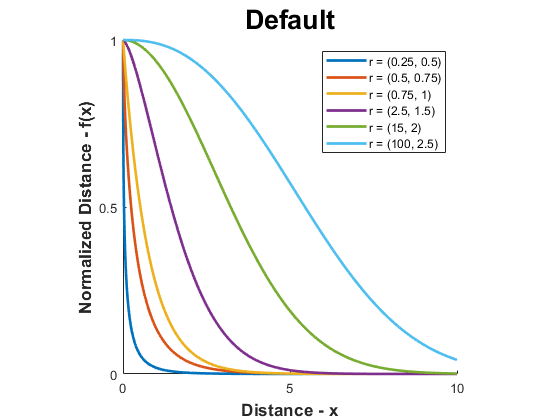
\includegraphics[scale=.5]{Fuzz1v1.png} \\
		 
	\item[\texttt{"sigmoid"/"modsampen"}]	$f(x) = (1+exp(\frac{x-r_2}{r_1}))^{-1}$\\ \ \\
		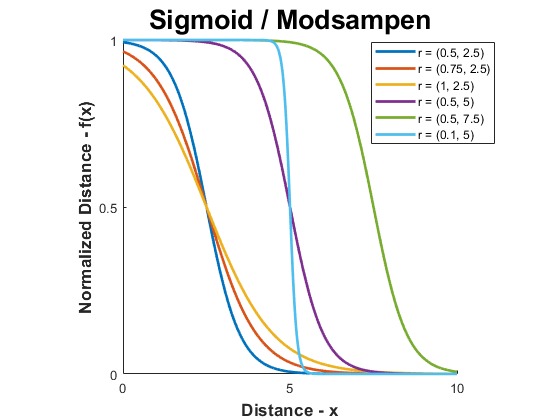
\includegraphics[scale=.5]{Fuzz2v1.png} \\

	\item[\texttt{"triangular"}]	  $f(x) = \begin{cases} 1 - \frac{x}{r},  \hspace{20mm}  x\le r 
	\\ 0,  \hspace{20mm}  x>r \end{cases}$\\
		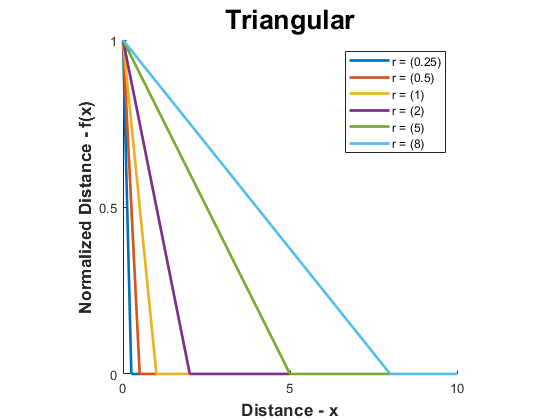
\includegraphics[scale=.5]{FuzzTriv1.png} \\

	\item[\texttt{"trapezoidal1"}]	  $f(x) = \begin{cases} 1,  \hspace{20mm}  x<r 
	\\ 2 - \frac{x}{r},  \hspace{10mm} r\le x<2r 
	\\ 0,  \hspace{20mm}  x\ge 2r \end{cases}$\\
		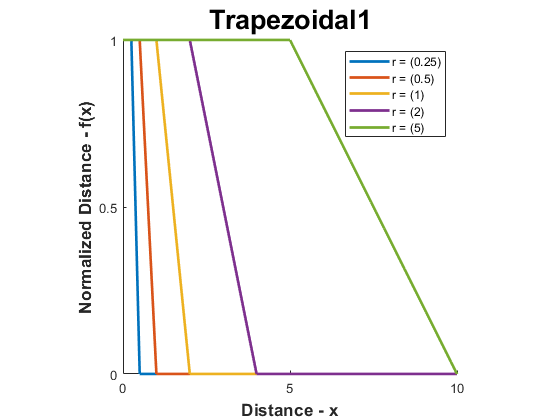
\includegraphics[scale=.5]{FuzzTrap1v1.png} \\ 

	\item[\texttt{"trapezoidal2"}]	  $f(x) = \begin{cases} 1,  \hspace{30mm}  x<r 
	\\ 1 - \frac{x-r_{min}}{r_{max} - r_{min}},  \hspace{5mm} r\le x<r_{max} 
	\\ 0,  \hspace{30mm}  x\ge r_{max} \end{cases}$\\ \ \\
		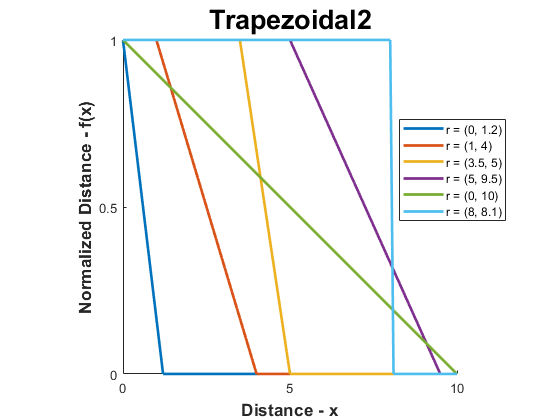
\includegraphics[scale=.5]{FuzzTrap2v1.png} \\ 
		
	\item[\texttt{"z\_shaped"}]	 $f(x) = \begin{cases} 1, \hspace{30mm}  x<r \\ \
	\\ 1 - 2 \left( \frac{x-r}{r}\right)^{2},  \hspace{10mm} r<x<\frac{3}{2}r \\ \
	\\ 2 \left( \frac{x-r}{r}\right)^{2},  \hspace{15mm} \frac{3}{2}r<x<2r \\ \
	\\ 0,  \hspace{30mm}  x>2r \end{cases}$ \\
		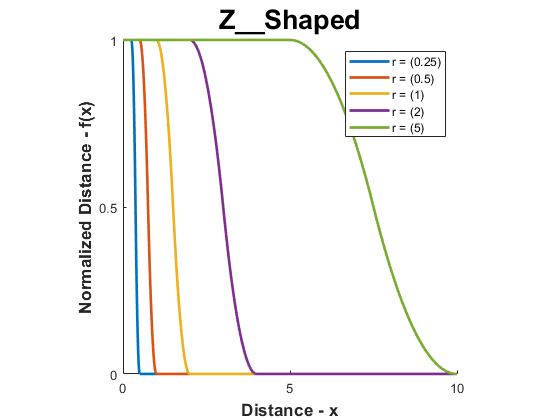
\includegraphics[scale=.5]{FuzzZSv1.png} \\
		
	\item[\texttt{"bell"}] $f\left( x \right) = \frac{1}{1+{\left |\frac{x}{r_1 }\right|}^{r_2 } }$ \\ 
		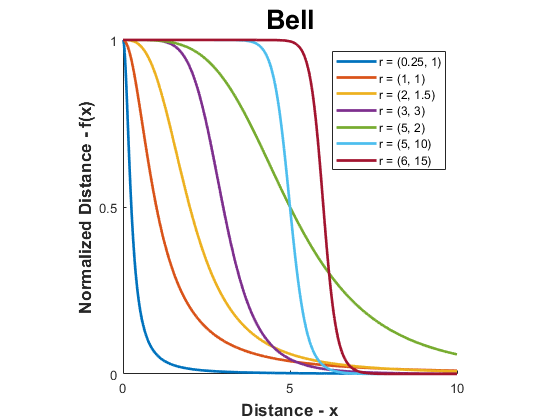
\includegraphics[scale=.5]{FuzzBv1.png}\\
				
	\item[\texttt{"gaussian"}] $f\left( x \right) = exp(-\frac{x^2}{2r^{2}})$ \\ 
		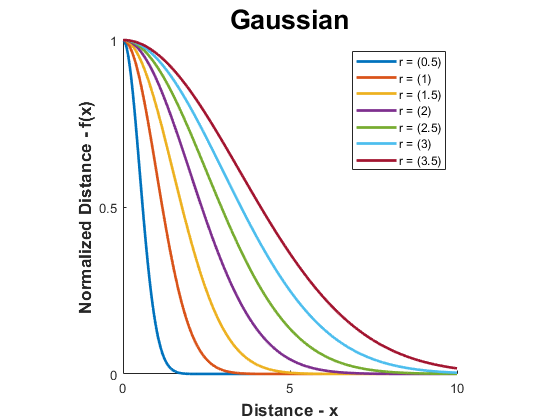
\includegraphics[scale=.5]{FuzzGaussv1.png} \\

	\item[\texttt{"constgaussian"}] $f(x) = \begin{cases} 1,  \hspace{35mm}  x<r_{min} 
	\\  exp(-\log(2)\frac{(x-r)^2}{r}),  \hspace{5mm}  x\ge r_{max} \end{cases}$\\
		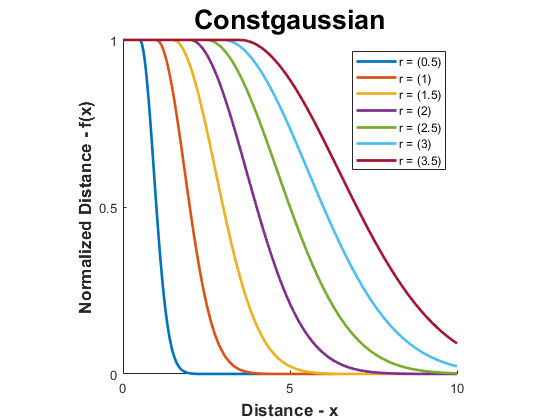
\includegraphics[scale=.5]{FuzzCGv1.png} \\

	\item[\texttt{"gudermannian"}] 	$g(x) = atan(\frac{tanh(r_1)}{x})$
	\item[]	$f(x) = \frac{g(x)}{g(x_{max})}$
	\item[]		Note: Distances are normalized w.r.t. maximum distance relative to each state vector.\\ \ \\
		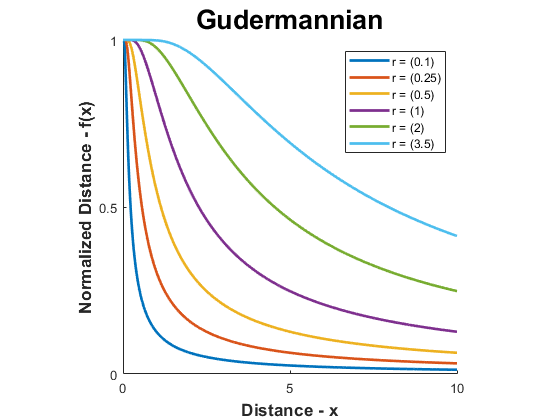
\includegraphics[scale=.5]{FuzzGv1.png} \\
	\end{description}
	
\item[\texttt{r}]	Parameters of the fuzzy function specified by \textbf{\texttt{Fx}}, a 1 element scalar or a 2 element tuple of positive values depending on the fuzzy function as shown above.
	\begin{description}[labelsep=14em, labelwidth=10em, nosep,style=multiline,leftmargin=3cm]
	\item[\texttt{\emph{Default}}]		Two element tuple (or vector in MatLab)
	\item[\texttt{\emph{Sigmoid/ModSampEn}}]		Two element tuple (or vector in MatLab)
	\item[\texttt{\emph{Trapezoidal2}}]		Two element tuple (or vector in MatLab)
	\item[\texttt{\emph{Bell}}]		Two element tuple (or vector in MatLab)
	\item[\texttt{\emph{Trapezoidal1}}]		 A scalar value
	\item[\texttt{\emph{Triangular}}]		 A scalar value
	\item[\texttt{\emph{Z\_Shaped}}]	 A scalar value
	\item[\texttt{\emph{Gaussian}}] A scalar value
	\item[\texttt{\emph{ConstGaussian}}] A scalar value
	\item[\texttt{\emph{Gudermannian}}] A scalar value
	\end{description}

\item[\texttt{Logx}]	Logarithm base in the entropy formula, a positive scalar.
\end{description}

\noindent \ul{Outputs}
\begin{description}[labelsep=1cm, labelwidth=2cm, nosep]\footnotesize
\item[\texttt{XFuzz}]	Cross-fuzzy entropy estimates for each embedding dimension from 1 to m.
\item[\texttt{Ps1}]		The average fuzzy distances for embedding dimensions from 1 to m.
\item[\texttt{Ps2}]		The average fuzzy distances for embedding dimensions from 2 to m+1.
\end{description}

\noindent \ul{References}\hspace{1cm}
\cite{XFuzz1} \cite{Fuzz3}



\newpage
\subsection{\normalsize XK2En: \hspace{15mm}  Cross-Kolmogorov Entropy}\label{XK2En}
\noindent\ul{Syntax} \vspace{6mm} \\ \noindent \texttt{\footnotesize
[XK2, Ci] = XK2En(Sig1, Sig2, ‘m’, 2, ‘tau’, 1, ‘r’, 0.2*std\textsubscript{pooled}(Sig1, Sig2), ‘Logx’, exp(1)) \\
XK2, Ci  = XK2En(Sig1, Sig2, m = 2, tau = 1, r = 0.2*std\textsubscript{pooled}(Sig1, Sig2), Logx = np.exp(1)) \\
XK2, Ci  = XK2En(Sig1, Sig2, m = 2, tau = 1, r = 0.2*std\textsubscript{pooled}(Sig1, Sig2), Logx = exp(1))}

\noindent \ul{Arguments}
\begin{description}[labelsep=1cm, labelwidth=2cm, nosep, style=multiline,leftmargin=3cm]\footnotesize
\item[\texttt{Sig1}]	First data sequence, a vector of $>10$ elements.
\item[\texttt{Sig2}]	Second data sequence, a vector of $>10$ elements.
\item[\texttt{m}]		Embedding dimension, a positive integer.
\item[\texttt{tau}]		Time delay, a positive integer.
\item[\texttt{r}]		Distance threshold value, a positive scalar.
\item[\texttt{Logx}]	Logarithm base in the entropy formula, a positive scalar.
\end{description}

\noindent \ul{Outputs}
\begin{description}[labelsep=1cm, labelwidth=2cm, nosep, style=multiline,leftmargin=3cm]\footnotesize
\item[\texttt{XK2}]		Cross-Kolmogorov entropy estimates for each embedding dimension from 1 to m
\item[\texttt{Ci}]		The correlation sum for each embedding dimension from 1 to m.
\end{description}

\noindent \ul{References}\hspace{1cm}
\cite{Matt1}



\newpage
\subsection{\normalsize XPermEn: \hspace{15mm} Cross-Permutation Entropy}
\noindent\ul{Syntax} \vspace{6mm} \\ \noindent \texttt{\footnotesize
[XPerm] = XPermEn(Sig1, Sig2, ‘m’, 3, ‘tau’, 1, ‘Logx’, 2)\\
 XPerm  = XPermEn(Sig1, Sig2, m = 3, tau = 1, Logx = 2)\\
 XPerm  = XPermEn(Sig1, Sig2, m = 3, tau = 1, Logx = 2)}

\noindent \ul{Arguments}
\begin{description}[labelsep=1cm, labelwidth=2cm, nosep,,style=multiline,leftmargin=3cm]\footnotesize
\item[\texttt{Sig1}]	First data sequence, a vector of $>10$ elements.
\item[\texttt{Sig2}]	Second data sequence, a vector of $>10$ elements.\\
\textbf{NOTE: \texttt{Sig1}} and \textbf{\texttt{Sig2}} must have the same number of elements.
\item[\texttt{m}]		Embedding dimension, an integer $> 2$.\\
\textbf{NOTE: \texttt{XPerm}} is undefined for \texttt{\textbf{m}} $< 3$.
\item[\texttt{tau}]		Time delay, a positive integer.
\item[\texttt{Logx}]	Logarithm base in the entropy formula, a positive scalar.\\
(Enter 0 for natural logarithm)
\end{description}

\noindent \ul{Outputs}
\begin{description}[labelsep=1cm, labelwidth=2cm, nosep, style=multiline,leftmargin=3cm]\footnotesize
\item[\texttt{XPerm}]		Cross-permutation entropy estimate.\\
\end{description}

\noindent \ul{References}\hspace{1cm}
\cite{XPerm1}



\newpage
\subsection{\normalsize XCondEn: \hspace{15mm} Cross-Conditional Entropy}
\noindent\ul{Syntax} \vspace{6mm} \\ \noindent \texttt{\footnotesize
[XCond, SEw, SEz] = XCondEn(Sig1, Sig2, ‘m’, 2, ‘tau’, 1, ‘c’, 6, ‘Logx’, exp(1), ‘Norm’, false)\\
XCond, SEw, SEz  = XCondEn(Sig1, Sig2, m = 2, tau = 1, c = 6, Logx = np.exp(1), Norm = False) \\
XCond, SEw, SEz  = XCondEn(Sig1, Sig2, m = 2, tau = 1, c = 6, Logx = exp(1), Norm = false)}

\noindent \ul{Arguments}
\begin{description}[labelsep=1cm, labelwidth=2cm, nosep, style=multiline,leftmargin=3cm]\footnotesize
\item[\texttt{Sig1}]	First data sequence, a vector of $>10$ elements.
\item[\texttt{Sig2}]	Second data sequence, a vector of $>10$ elements.\\
\textbf{NOTE: \texttt{Sig1}} and \textbf{\texttt{Sig2}} must have the same number of elements.\\
\textbf{NOTE: \ul{XCondEn}} is direction-dependent. Therefore, the order of the data sequences in \texttt{\textbf{Sig}} matters. If the first column of \texttt{\textbf{Sig}} is the
    sequence 'y', and the second column is the sequence 'u', \texttt{\textbf{XCond}} is  the amount of information carried by y(i) when the pattern u(i) is found.
\item[\texttt{m}]		Embedding dimension, an integer $> 1$.
\item[\texttt{tau}]		Time delay, a positive integer.
\item[\texttt{c}]		Number of symbols in symbolic transformation, in integer $> 1$
\item[\texttt{Logx}]	Logarithm base in the entropy formula, a positive scalar.
\item[\texttt{Norm}]	Normalization of \texttt{\textbf{XCond}} value:\\
		  \texttt{true} \hspace{15pt}  no normalisation (default)\\
		  \texttt{false} \hspace{10pt}  normalises w.r.t cross-Shannon entropy.
\end{description}

\noindent \ul{Outputs}
\begin{description}[labelsep=1cm, labelwidth=2cm, nosep, style=multiline,leftmargin=3cm]\footnotesize
\item[\texttt{XCond}]		Corrected Cross-Conditional entropy estimate.
\item[\texttt{SEw}]		Cross-Shannon entropy estimate for \texttt{\textbf{m}}.
\item[\texttt{SEz}]		Cross-Shannon entropy estimate for \texttt{\textbf{m+1}}.
\end{description}

\noindent \ul{References}\hspace{1cm}
\cite{Cond1}



\newpage
\subsection{\normalsize XDistEn: \hspace{15mm} Cross-Distribution Entropy}
\noindent\ul{Syntax} \vspace{6mm} \\ \noindent \texttt{\footnotesize
[XDist, Ppi] = XDistEn(Sig1, Sig2, ‘m’, 2, ‘tau’, 1, ‘Bins’, ‘sturges’, ‘Logx’, 2, ‘Norm’, true)\\
XDist, Ppi  = XDistEn(Sig1, Sig2, m = 2, tau = 1, Bins = ‘sturges’, Logx = 2, Norm = True)\\ 
XDist, Ppi  = XDistEn(Sig1, Sig2, m = 2, tau = 1, Bins = "sturges", Logx = 2, Norm = true)}

\noindent \ul{Arguments}
\begin{description}[labelsep=1cm, labelwidth=2cm, nosep, style=multiline,leftmargin=3cm]\footnotesize
\item[\texttt{Sig1}]	First data sequence, a vector of $>10$ elements.
\item[\texttt{Sig2}]	Second data sequence, a vector of $>10$ elements.
\item[\texttt{m}]		Embedding dimension, an integer $> 1$.
\item[\texttt{tau}]		Time delay, a positive integer.
\item[\texttt{Bins}]	Histogram bin selection method, in integer $> 1$ indicating the number of bins, 
						or one of the following strings:\\
   					    "sturges", "sqrt", "rice", "doanes" \hspace{2em} [default: "sturges"]
\\ \href{https://en.wikipedia.org/wiki/Histogram#Number_of_bins_and_width}{$>>>$ More info on binning methods}.
\item[\texttt{Logx}]	Logarithm base in the entropy formula, a positive scalar.\\
						(Enter 0 for natural logarithm)
\item[\texttt{Norm}]	Normalization of \texttt{\textbf{XDist}} value:\\
		  \texttt{false} \hspace{10pt} no normalisation \\
		  \texttt{true} \hspace{15pt} normalises w.r.t number of histogram bins (default)
\end{description}

\noindent \ul{Outputs}
\begin{description}[labelsep=1cm, labelwidth=2cm, nosep, style=multiline,leftmargin=3cm]\footnotesize
\item[\texttt{XDist}]		Cross-Distribution entropy estimate.
\item[\texttt{Ppi}]		Probability of each histogram bin.
\end{description}

\noindent \ul{References}\hspace{1cm}
\cite{Dist1}



\newpage
\subsection{\normalsize XSpecEn: \hspace{15mm} Cross-Spectral Entropy}
\noindent\ul{Syntax} \vspace{6mm} \\ \noindent \texttt{\footnotesize
[XSpec, BandEn] = XSpecEn(Sig1, Sig2, ‘N’, 2*max(length(Sig1), length(Sig2))+1, ‘Freqs’, [0,1], ‘Logx’, exp(1), ‘Norm’, true)\\
XSpec, BandEn  = XSpecEn(Sig1, Sig2, N = 2*np.maximum(len(Sig1),len(Sig2)) + 1, Freqs = (0,1), Logx = np.exp(1), Norm = True)\\ 
XSpec, BandEn  = XSpecEn(Sig, N = 2*max(length(Sig1),length(Sig2)) + 1, Freqs = (0,1), Logx = exp(1), Norm = true)}

\noindent \ul{Arguments}
\begin{description}[labelsep=1cm, labelwidth=2cm, nosep, style=multiline,leftmargin=3cm]\footnotesize
\item[\texttt{Sig1}]	First data sequence, a vector of $>10$ elements.
\item[\texttt{Sig2}]	Second data sequence, a vector of $>10$ elements.
\item[\texttt{N}]		Resolution of the N-point fft, an integer $> 1$.
\item[\texttt{Freqs}]	Normalised band edge-frequencies for calculating the band entropy (BandEn), a 2 element tuple with values in range [0, 1] where 1 is the Nyquist frequency. \\
		* When no edge frequencies are provided, BandEn==XSpecEn
\item[\texttt{Logx}]	Logarithm base in the entropy formula, a positive scalar.
\item[\texttt{Norm}]	Normalization of \texttt{\textbf{XSpec}} value:\\
		  \texttt{false} \hspace{10pt} no normalisation \\
		  \texttt{true} \hspace{15pt}  normalises \texttt{\textbf{XSpec}} w.r.t number of Nyquist frequency values, and \texttt{\textbf{BandEn}} w.r.t. range of frequencies in the band given by \texttt{\textbf{Freqs}}. (default)
\end{description}

\noindent \ul{Outputs}
\begin{description}[labelsep=1cm, labelwidth=2cm, nosep, style=multiline,leftmargin=3cm]\footnotesize
\item[\texttt{XSpec}]		Cross-Spectral entropy estimate.
\item[\texttt{BandEn}]		Cross-Spectral band entropy estimate.
\end{description}

\noindent \ul{References}\hspace{1cm}
\cite{Matt1}
\\ \ \\
\noindent\ul{\textbf{Note:}}\hspace{5mm} In contrast to other \textit{Cross-}entropies, cross-spectral entropy (XSpecEn) is not derived from information theory or dynamical systems theory, and instead is an estimate of the frequency cross-spectrum curve estimated using the discrete time Fourier transform.


%------------------------------------------------------------------------
%------------------------------------------------------------------------

\newpage
\section{Multivariate Entropy Functions}
\vspace{8cm}

\begin{tcolorbox}[colback=ehone!5, colframe=ehtwo!, title=\hypertarget{bidinote}{\textbf{Multivariate Data}}, label={BiBox}]
Unlike \textit{Base} and \textit{Cross-} entropy functions, \textit{\textbf{Multivariate}} entropy functions operate on a matrix of univariate sequences. This, in the following functions, the first argument \texttt{\textbf{Data}} is an N x M matrix representing M ($> 1$) univariate sequences of N ($> 10$) samples.
\end{tcolorbox}
\vspace{2cm}
\begin{tcolorbox}[colback=ehone!5, colframe=ehtwo!, title=\hypertarget{bidinote}{\textbf{ATTENTION}}, label={BiBox}]
By default, the \texttt{\textbf{MvSampEn}} and \texttt{\textbf{MvFuzzEn}} multivariate entropy algorithms estimate entropy values using the “full” method by comparing delay vectors across all possible m+1 expansions of the embedding space as applied in \cite{MvSamp1} \cite{MvSamp2} \cite{MvFuzz1}. These methods are \ul{\textbf{not lower-bounded to 0}}, like most entropy algorithms, so \texttt{\textbf{MvMSEn}} may return negative entropy values if the base multivariate entropy function is \texttt{\textbf{MvSampEn}} and \texttt{\textbf{MvFuzzEn}}, even for stochastic processes…
\end{tcolorbox}


\newpage
\subsection{\normalsize MvSampEn: \hspace{15mm} Multivariate Sample Entropy} \label{MvSampEn}
\noindent\ul{Syntax} \vspace{6mm} \\ \noindent \texttt{\footnotesize
[MSamp, B0, Bt, B1] = MvSampEn(Data, ‘m’, 2*ones(1,size(Data,2)), \\ \indent ‘tau’, ones(1,size(Data,2)), ‘r’, 0.2, 'Norm', false, ‘Logx’, exp(1))\\
 MSamp, B0, Bt, B1  = MvSampEn(Data, m = 2*np.ones(Data.shape[1]),  \\ \indent tau = np.ones(Data.shape[1]), r = 0.2, Norm = False, Logx = np.exp(1))\\
 MSamp, B0, Bt, B1  = MvSampEn(Data, m = 2*ones(size(Data,2)),  \\ \indent tau = ones(size(Data,2)), r = 0.2, Norm = false Logx = exp(1))}
 
\begin{tcolorbox}[colback=ehone!5, colframe=ehtwo!, title=\hypertarget{bidinote}{\textbf{NOTE}}, label={BiBox}]
To maximize the number of points in the embedding process, this algorithm uses \texttt{\textbf{N-max(m*tau)}} delay vectors and \textbf{not} \texttt{\textbf{N-max(m)*max(tau)}} as employed in \cite{MvSamp2},\cite{MvSamp1}.
\end{tcolorbox}

\noindent \ul{Arguments}
\begin{description}[labelsep=1cm, labelwidth=2cm, nosep,,style=multiline,leftmargin=3cm]\footnotesize
\item[\texttt{Data}]	Multivariate dataset, NxM matrix of N ($>10$) observations (rows) and M ($> 1$) univariate data sequences (cols).
\item[\texttt{m}]		Embedding Dimension, a vector of M positive integers.
\item[\texttt{tau}]		Time Delay, a vector of M positive integers.
\item[\texttt{r}]		Distance threshold, a positive scalar.
\item[\texttt{Norm}]	Normalisation of all M sequences to unit variance, a boolean
\item[\texttt{Logx}]	Logarithm base in the entropy formula, a positive scalar.
\end{description}

\noindent \ul{Outputs}
\begin{description}[labelsep=1cm, labelwidth=2cm, nosep, style=multiline,leftmargin=3cm]\footnotesize
\item[\texttt{MSamp}]		Multivariate sample entropy estimates.
\item[\texttt{B0}]		The number of matched state vectors for given m embedding dimensions.
\item[\texttt{Bt}]		 The number of matched state vectors for the joint total m+1 embedded subspace.
\item[\texttt{B1}]		The number of matched state vectors for each possible m+1 embedded subspace.
\end{description}          

\noindent \ul{References}\hspace{1cm}
\cite{MvSamp1}  \cite{MvSamp2}


\newpage
\subsection{\normalsize MvFuzzEn: \hspace{15mm} Multivariate Fuzzy Entropy} \label{MvFuzzEn}
\noindent\ul{Syntax} \vspace{6mm} \\ \noindent \texttt{\footnotesize
[MFuzz, B0, Bt, B1] = MvFuzzEn(Data, ‘m’, 2*ones(1,size(Data,2)), \\ \indent ‘tau’, ones(1,size(Data,2)), 'Fx', 'default', ‘r’, [0.2,2], \\ \indent 'Norm', false, ‘Logx’, exp(1))\\
 MFuzz, B0, Bt, B1  = MvFuzzEn(Data, m = 2*np.ones(Data.shape[1]), \\ \indent tau = np.ones(Data.shape[1]), Fx = 'default', r = (0.2,2), \\ \indent Norm = False, Logx = np.exp(1))\\
 MFuzz, B0, Bt, B1  = MvFuzzEn(Data, m = 2*ones(size(Data,2)), \\ \indent tau = ones(size(Data,2)), Fx = "default", r = (0.2,2), \\ \indent Norm = false, Logx = exp(1))}
 
\begin{tcolorbox}[colback=ehone!5, colframe=ehone!, title=\hypertarget{bidinote}{\textbf{IMPORTANT}}, label={BiBox}]
The entropy value returned as \texttt{\textbf{MFuzz}} is estimated using the “full” method [i.e. \texttt{-log(Bt/B0)]} which compares delay vectors across all possible m+1 expansions of the embedding space as applied in \cite{MvSamp1}. Contrary to conventional definitions of fuzzy entropy, this method does not provide a lower bound of 0!! Thus, it is possible to obtain negative entropy values for multivariate fuzzy entropy, even for stochastic processes…
\newline
Alternatively, one can calculate \texttt{\textbf{MFuzz}} via the “naive” method, which ensures a lower bound of 0, by using the average vector distances for an individual m+1 subspace (B1) [e.g. \texttt{-log(B1(1)/B0)}], or the average for all m+1 subspaces [i.e. \texttt{-log(mean(B1)/B0)}].
\end{tcolorbox} 

\begin{tcolorbox}[colback=ehone!5, colframe=ehtwo!, title=\hypertarget{bidinote}{\textbf{NOTE}}, label={BiBox}]
To maximize the number of points in the embedding process, this algorithm uses \texttt{\textbf{N-max(m*tau)}} delay vectors and \textbf{not} \texttt{\textbf{N-max(m)*max(tau)}} as employed in \cite{MvSamp2},\cite{MvSamp1}.
\end{tcolorbox} 
 
\noindent \ul{Arguments}
\begin{description}[labelsep=1cm, labelwidth=2cm, nosep,,style=multiline,leftmargin=3cm]\footnotesize
\item[\texttt{Data}]	Multivariate dataset, NxM matrix of N ($>10$) observations (rows) and M ($> 1$) univariate data sequences (cols).
\item[\texttt{m}]		Embedding Dimension, a vector of M positive integers.
\item[\texttt{tau}]		Time Delay, a vector of M positive integers. 
\item[\texttt{Fx}]		Type of fuzzy function for distance transformation, one of the following strings:
	\begin{description}[labelsep=14em, labelwidth=10em, nosep,style=multiline,leftmargin=6cm]
	\item[\texttt{"default"}]	$f(x) = exp(-\frac{x^{r_2}}{r_1})$\\ \ \\
		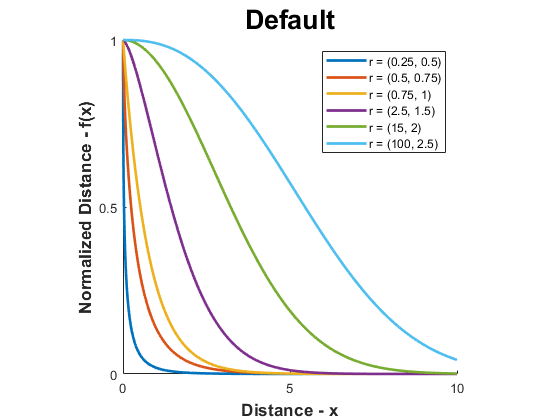
\includegraphics[scale=.5]{Fuzz1v1.png} \\
		 
	\item[\texttt{"sigmoid"/"modsampen"}]	$f(x) = (1+exp(\frac{x-r_2}{r_1}))^{-1}$\\ \ \\
		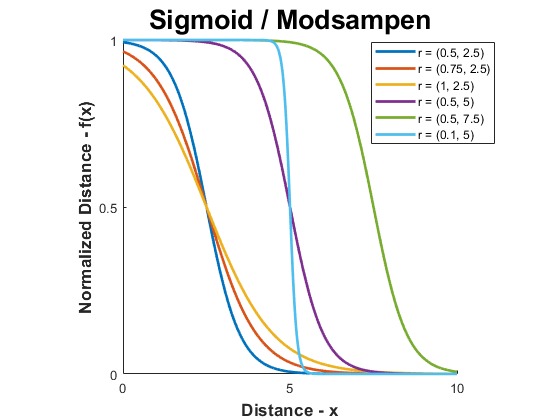
\includegraphics[scale=.5]{Fuzz2v1.png} \\

	\item[\texttt{"triangular"}]	  $f(x) = \begin{cases} 1 - \frac{x}{r},  \hspace{20mm}  x\le r 
	\\ 0,  \hspace{20mm}  x>r \end{cases}$\\
		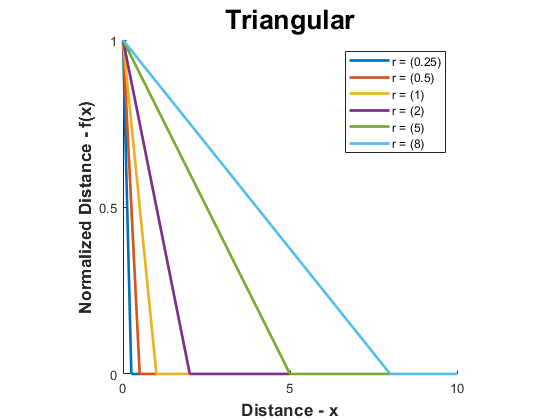
\includegraphics[scale=.5]{FuzzTriv1.png} \\

	\item[\texttt{"trapezoidal1"}]	  $f(x) = \begin{cases} 1,  \hspace{20mm}  x<r 
	\\ 2 - \frac{x}{r},  \hspace{10mm} r\le x<2r 
	\\ 0,  \hspace{20mm}  x\ge 2r \end{cases}$\\
		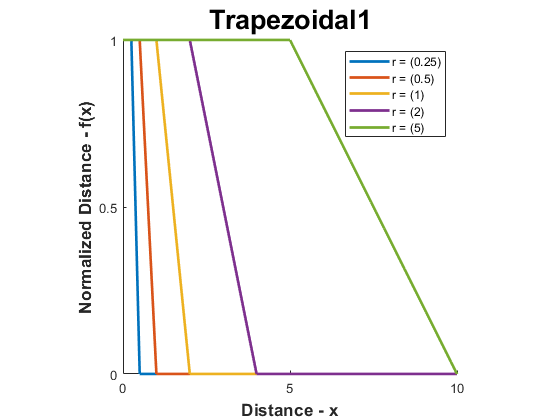
\includegraphics[scale=.5]{FuzzTrap1v1.png} \\ 

	\item[\texttt{"trapezoidal2"}]	  $f(x) = \begin{cases} 1,  \hspace{30mm}  x<r 
	\\ 1 - \frac{x-r_{min}}{r_{max} - r_{min}},  \hspace{5mm} r\le x<r_{max} 
	\\ 0,  \hspace{30mm}  x\ge r_{max} \end{cases}$\\ \ \\
		\includegraphics[scale=.5]{FuzzTrap2v1.png} \\ 
		
	\item[\texttt{"z\_shaped"}]	 $f(x) = \begin{cases} 1, \hspace{30mm}  x<r \\ \
	\\ 1 - 2 \left( \frac{x-r}{r}\right)^{2},  \hspace{10mm} r<x<\frac{3}{2}r \\ \
	\\ 2 \left( \frac{x-r}{r}\right)^{2},  \hspace{15mm} \frac{3}{2}r<x<2r \\ \
	\\ 0,  \hspace{30mm}  x>2r \end{cases}$ \\
		\includegraphics[scale=.5]{FuzzZSv1.png} \\
		
	\item[\texttt{"bell"}] $f\left( x \right) = \frac{1}{1+{\left |\frac{x}{r_1 }\right|}^{r_2 } }$ \\ 
		\includegraphics[scale=.5]{FuzzBv1.png}\\
				
	\item[\texttt{"gaussian"}] $f\left( x \right) = exp(-\frac{x^2}{2r^{2}})$ \\ 
		\includegraphics[scale=.5]{FuzzGaussv1.png} \\

	\item[\texttt{"constgaussian"}] $f(x) = \begin{cases} 1,  \hspace{35mm}  x<r_{min} 
	\\  exp(-\log(2)\frac{(x-r)^2}{r}),  \hspace{5mm}  x\ge r_{max} \end{cases}$\\
		\includegraphics[scale=.5]{FuzzCGv1.png} \\

	\item[\texttt{"gudermannian"}] 	$g(x) = atan(\frac{tanh(r_1)}{x})$
	\item[]	$f(x) = \frac{g(x)}{g(x_{max})}$
	\item[]		Note: Distances are normalized w.r.t. maximum distance relative to each state vector.\\ \ \\
		\includegraphics[scale=.5]{FuzzGv1.png} \\
	\end{description}
	
\item[\texttt{r}]	Parameters of the fuzzy function specified by \textbf{\texttt{Fx}}, a 1 element scalar or a 2 element tuple of positive values depending on the fuzzy function as shown above.
	\begin{description}[labelsep=14em, labelwidth=10em, nosep,style=multiline,leftmargin=3cm]
	\item[\texttt{\emph{Default}}]		Two element tuple (or vector in MatLab)
	\item[\texttt{\emph{Sigmoid/ModSampEn}}]		Two element tuple (or vector in MatLab)
	\item[\texttt{\emph{Trapezoidal2}}]		Two element tuple (or vector in MatLab)
	\item[\texttt{\emph{Bell}}]		Two element tuple (or vector in MatLab)
	\item[\texttt{\emph{Trapezoidal1}}]		 A scalar value
	\item[\texttt{\emph{Triangular}}]		 A scalar value
	\item[\texttt{\emph{Z\_Shaped}}]	 A scalar value
	\item[\texttt{\emph{Gaussian}}] A scalar value
	\item[\texttt{\emph{ConstGaussian}}] A scalar value
	\item[\texttt{\emph{Gudermannian}}] A scalar value
	\end{description}
\item[\texttt{Norm}]	Normalisation of all M sequences to unit variance, a boolean
\item[\texttt{Logx}]	Logarithm base in the entropy formula, a positive scalar.
\end{description}

\noindent \ul{Outputs}
\begin{description}[labelsep=1cm, labelwidth=2cm, nosep, style=multiline,leftmargin=3cm]\footnotesize
\item[\texttt{MFuzz}]		Multivariate fuzzy entropy estimates.
\item[\texttt{B0}]		Average delay vector distance for given m embedding dimensions.
\item[\texttt{Bt}]		Average delay vector distance for the joint total m+1 embedded subspace.
\item[\texttt{B1}]		Average delay vector distance for each possible m+1 embedded subspace.
\end{description} 

\noindent \ul{References}\hspace{1cm}
\cite{MvFuzz1}


\newpage
\subsection{\normalsize MvDispEn: \hspace{15mm} Multivariate Dispersion Entropy} \label{MvDispEn}
\noindent\ul{Syntax} \vspace{6mm} \\ \noindent \texttt{\footnotesize
[MDisp, RDE] = MvDispEn(Data, ‘m’, 2*ones(1,size(Data,2)),  \\ \indent ‘tau’, ones(1,size(Data,2)), 'c', 3, ‘Typex’, 'NCDF', 'Methodx', 'v1', \\ \indent 'Norm', false, ‘Logx’, exp(1))\\
 MDisp, RDE  = MvDispEn(Data, m = 2*np.ones(Data.shape[1]),  \\ \indent  tau = np.ones(Data.shape[1]), c = 3, Typex = 'NCDF', Methodx = 'v1', \\ \indent Norm = False, Logx = np.exp(1))\\
 MDisp, RDE  = MvDispEn(Data, m = 2*ones(size(Data,2)),   \\ \indent  tau = ones(size(Data,2)), c = 3, Typex = "NCDF", Methodx = "v1", \\ \indent Norm = false, Logx = exp(1))} 
 
\begin{tcolorbox}[colback=ehone!5, colframe=ehtwo!, title=\hypertarget{bidinote}{\textbf{IMPORTANT}}, label={BiBox}]
By default, \texttt{MvDispEn} uses the method termed  \textit{\textbf{mvDEii}} in \cite{MvDisp1}, which follows the original multivariate embedding approach of Ahmed \& Mandic \cite{MvSamp1}, \cite{MvSamp2}. The \textit{\textbf{v1}} method therefore returns a singular entropy estimate.\\ \newline
If the \textit{\textbf{v2}} method is selected (\texttt{Methodx=='v2'}), the main method outlined in \cite{MvDisp1} termed \textit{\textbf{mvDE}} is applied. In this case, entropy is estimated using each combination of multivariate delay vectors with lengths 1:max(m), with each entropy value returned accordingly. See \cite{MvDisp1} for more info.
\end{tcolorbox}
 
\noindent \ul{Arguments}
\begin{description}[labelsep=1cm, labelwidth=2cm, nosep,,style=multiline,leftmargin=3cm]\footnotesize
\item[\texttt{Data}]	Multivariate dataset, NxM matrix of N ($>10$) observations (rows) and M ($> 1$) univariate data sequences (cols).
\item[\texttt{m}]		Embedding Dimension, a vector of M positive integers.
\item[\texttt{tau}]		Time Delay, a vector of M positive integers. 
\item[\texttt{c}]		Number of symbols in transform, an integer $> 1$. 
\item[\texttt{Typex}]	Type of symbolic sequence transform, one of the following strings:
	\begin{description}[labelsep=5em, labelwidth=8em, nosep,style=multiline,leftmargin=3cm]
		\item[\texttt{"ncdf"}]		Normalised cumulative distribution function  \cite{Disp1}		
		\item[\texttt{"kmeans"}] 	K-means clustering algorithm.\\
		**Note: The \textit{"kmeans"} algorithm uses random initialization conditions.
		 This causes results to vary slightly each time it is called.
		\item[\texttt{"linear"}]	Linear segmentation of signal range 
		\item[\texttt{"equal"}]		Approx. equal number of symbols.
		\item[]		\includegraphics[scale=.75]{Disp1.png}
	\end{description}
\item[\texttt{Methodx}]		The method of multivariate dispersion entropy estimation as outlined in \cite{MvDispEn1}, either: 
	\begin{description}[labelsep=5em, labelwidth=8em, nosep,style=multiline,leftmargin=3cm]
\item[\texttt{"v1"}]    employs the method consistent with the original multivariate embedding approach of Ahmed \& Mandic \cite{MvDispEn2}, termed \textbf{\texttt{mvDEii}} in \cite{MvDispEn1}. (default) 
\item[\texttt{"v2"}]    employs the main method derived in \cite{MvDispEn1}, termed \textbf{\texttt{mvDE}}.
	\end{description}
\item[\texttt{Norm}]	Normalisation of MDisp value w.r.t. the number of unique dispersion patterns, a boolean
\item[\texttt{Logx}]	Logarithm base in the entropy formula, a positive scalar.
\end{description}

\noindent \ul{Outputs}
\begin{description}[labelsep=1cm, labelwidth=2cm, nosep, style=multiline,leftmargin=3cm]\footnotesize
\item[\texttt{MDisp}]		Multivariate dispersion entropy estimates.
\item[\texttt{RDE}]		Multivariate reverse dispersion entropy estimate.
\end{description} 

\noindent \ul{References}\hspace{1cm}
\cite{MvDisp1}




\newpage
\subsection{\normalsize MvPermEn: \hspace{15mm} Multivariate Permutation Entropy} \label{MvPermEn}
\noindent\ul{Syntax} \vspace{6mm} \\ \noindent \texttt{\footnotesize
[MPerm, MPnorm] = MvPermEn(Data, ‘m’, 2*ones(1,size(Data,2)),  \\ \indent ‘tau’, ones(1,size(Data,2)), ‘Typex’, [], 'tpx', -1,\\ \indent 'Norm', false, ‘Logx’, 2)\\
 MPerm, MPnorm  = MvPermEn(Data, m = 2*np.ones(Data.shape[1]),  \\ \indent tau = np.ones(Data.shape[1]), Typex = None, tpx = -1, \\ \indent Norm = False, Logx = 2)\\
 MPerm, MPnorm  = MvPermEn(Data, m = 2*ones(size(Data,2)), \\ \indent tau = ones(size(Data,2)), Typex = nothing, tpx = -1, \\ \indent Norm = false, Logx = 2)} 
 
 
\begin{tcolorbox}[colback=ehone!5, colframe=ehone!, title=\hypertarget{bidinote}{\textbf{IMPORTANT}}, label={BiBox}]
The multivariate permutation entropy algorithm implemented here uses multivariate embedding based on Takens’ embedding theorem, and follows the methods for multivariate entropy estimation through shared spatial reconstruction as originally presented by Ahmed \& Mandic \cite{MvSamp1} \cite{MvSamp2}.
\newline
This function does \textbf{NOT} use the multivariate permutation entropy algorithm of Morabito et al. (Entropy, 2012) where the entropy values of individual univariate sequences are averaged because such methods do not follow the definition of multivariate embedding and therefore do not consider cross-channel statistical complexity.
\end{tcolorbox} 

\begin{tcolorbox}[colback=ehone!5, colframe=ehtwo!, title=\hypertarget{bidinote}{\textbf{NOTE}}, label={BiBox}]
To maximize the number of points in the embedding process, this algorithm uses \texttt{\textbf{N-max(m*tau)}} delay vectors and \textbf{not} \texttt{\textbf{N-max(m)*max(tau)}} as employed in \cite{MvSamp2},\cite{MvSamp1}.
\end{tcolorbox} 

 
\noindent \ul{Arguments}
\begin{description}[labelsep=1cm, labelwidth=2cm, nosep,,style=multiline,leftmargin=3cm]\footnotesize
\item[\texttt{Data}]	Multivariate dataset, NxM matrix of N ($>10$) observations (rows) and M ($> 1$) univariate data sequences (cols).
\item[\texttt{m}]		Embedding Dimension, a vector of M positive integers.
\item[\texttt{tau}]		Time Delay, a vector of M positive integers. 
\item[\texttt{Typex}]	Variant of permutation entropy, one of the following strings:
	\begin{description}[labelsep=10em, labelwidth=6em, nosep,style=multiline,leftmargin=3cm]
		\item[\texttt{"modified"}] 	Modified permutation entropy \cite{Perm3}
		\item[\texttt{"weighted"}]	Weighted permutation entropy \cite{Perm4}
		\item[\texttt{"ampaware"}]	Amplitude-aware permutation entropy \cite{Perm5}
		\item[\texttt{"edge"}]		Edge permutation entropy  \cite{Perm6}
		\item[\texttt{"phase"}]  Phase permutation entropy \cite{Perm9}
	\end{description}
\item[\texttt{tpx}]		Tuning parameter for the permutation entropy specified by the  \textbf{\texttt{Typex}} argument.
	\begin{description}[labelsep=10em, labelwidth=4em, nosep,style=multiline,leftmargin=3cm]	
	\item[\texttt{\emph{ampaware}}]	\textbf{\texttt{tpx}} is the A parameter, a value in range [0 1]  (default: 0.5)
	\item[\texttt{\emph{edge}}]	\textbf{\texttt{tpx}} is the r sensitivity parameter, a scalar $> 0$ (default: 1)	
	\item[\texttt{\emph{phase}}]	\textbf{\texttt{tpx}} is the option to unwrap the phase shift of the Hilbert-transformed data sequence, either [\ ] or 1 (default: [\ ]).		
	\end{description}
\item[\texttt{Norm}]    Normalisation of \texttt{\textbf{MPnorm}} value, a boolean operator:\\
					\texttt{false} \hspace{10pt} normalises w.r.t $Log$($\#$ of permutation symbols [\texttt{sum(m)}]) - default\\
     		  		\texttt{true} \hspace{15pt} normalises w.r.t $Log$($\#$ of all possible permutations [\texttt{sum(m)!]})
\item[\texttt{Logx}]	Logarithm base in the entropy formula, a positive scalar.
\end{description}

\noindent \ul{Outputs}
\begin{description}[labelsep=1cm, labelwidth=2cm, nosep, style=multiline,leftmargin=3cm]\footnotesize
\item[\texttt{MPerm}]	 Multivariate permutation entropy estimate
\item[\texttt{MPnorm}]		Normalized multivariate permutation entropy estimates.
\end{description} 

\noindent \ul{References}\hspace{1cm}
\cite{Matt1} \cite{MvSamp1}




\newpage
\subsection{\normalsize MvCoSiEn: \hspace{15mm} Multivariate Cosine Similarity Entropy}\label{MvCoSiEn}
\noindent\ul{Syntax} \vspace{6mm} \\ \noindent \texttt{\footnotesize
[MCoSi, Bm] = MvCoSiEn(Data, ‘m’, 2*ones(1,size(Data,2)), \\ \indent ‘tau’, ones(1,size(Data,2)), ‘r’, 0.1, ‘Logx’, 2, 'Norm', 0) \\
MCoSi, Bm  = MvCoSiEn(Data, m = 2*np.ones(Data.shape[1]),  \\ \indent tau = np.ones(Data.shape[1]), r = 0.1, Logx = 2, Norm = 0) \\
MCoSi, Bm  = MvCoSiEn(Data, m = 2*ones(size(Data,2)), \\ \indent tau = ones(size(Data,2)), r = 0.1, Logx = 2, Norm = 0)}

\begin{tcolorbox}[colback=ehone!5, colframe=ehtwo!, title=\hypertarget{bidinote}{\textbf{NOTE}}, label={BiBox}]
To maximize the number of points in the embedding process, this algorithm uses \texttt{\textbf{N-max(m*tau)}} delay vectors and \textbf{not} \texttt{\textbf{N-max(m)*max(tau)}} as employed in \cite{MvCoSi1},\cite{MvSamp1}.
\end{tcolorbox}

\noindent \ul{Arguments}
\begin{description}[labelsep=1cm, labelwidth=2cm, nosep, style=multiline,leftmargin=3cm]\footnotesize
\item[\texttt{Data}]	Multivariate dataset, NxM matrix of N ($>10$) observations (rows) and M ($> 1$) univariate data sequences (cols).
\item[\texttt{m}]		Embedding Dimension, a vector of M positive integers.
\item[\texttt{tau}]		Time Delay, a vector of M positive integers.
\item[\texttt{r}]		Angular threshold, a value in range [0 $<$ \texttt{\textbf{r}} $<$ 1]
\item[\texttt{Logx}]	Logarithm base in the entropy formula, a positive scalar.
\item[\texttt{Norm}]	Normalisation of each sequence in \texttt{\textbf{Data}}, an integer in range [0 4]:\\
						0 - no normalisation (default)\\
						1 - median removed\\
						2 - mean removed\\
						3 - normalised by unit variance\\
						4 - normalised to range [-1 1]
\end{description}

\noindent \ul{Outputs}
\begin{description}[labelsep=1cm, labelwidth=2cm, nosep, style=multiline,leftmargin=3cm]\footnotesize
\item[\texttt{MCoSi}]	Multivariate cosine similarity entropy  estimate.
\item[\texttt{Bm}]	Sum of global probabilities.
\end{description}

\noindent \ul{References}\hspace{1cm}
\cite{CoSi1} \cite{MvCoSi1}







%------------------------------------------------------------------------
%------------------------------------------------------------------------
\newpage
\section{Multiscale Entropy Functions}
\vspace{3em}

A key advantage of the EntropyHub toolkit is that so many variants of multiscale entropy can be easily
calculated using any of the \texttt{\textbf{Base}} entropy functions.  This is achieved using a multiscale entropy object (\texttt{\textbf{Mobj}}), returned by \texttt{\textbf{MSobject()}}, to specify the type of entropy and its parameters.
\begin{center}
\tcbox[tikznode={align=left}, colframe=ehone]{
\ul{Multiscale entropy functions have two positional arguments:} 
\\ \
\hspace{50pt} the time series signal \texttt{\textbf{Sig}}, and\\
\hspace{48pt} the multiscale entropy object, \texttt{\textbf{Mobj}}. }
\end{center}
 
\noindent Examples (shown in Julia syntax)$\colon$ \footnotesize
\\ \ \\ \noindent \emph{\textbf{Original multiscale entropy}} \cite{MS1}
\\ \ \\ \indent \texttt{Mobj = MSobject(SampEn) \\
\indent mse = MSEn(Sig, Mobj)}

\noindent \emph{\textbf{Time-shifted multiscale approximate entropy with varying tolerance across scales}} \cite{MS2} \\
\\ \ \indent \texttt{Mobj = MSobject(ApEn, m = 5, r = 0.25)\\
\indent mse = MSEn(Sig, Mobj, Methodx = "timeshift", RadNew = 1)}

\noindent \emph{\textbf{Composite multiscale conditional entropy with a 10-symbol data sequence, calculated up to 5 temporal scales}} \cite{cMS1}
\\ \ \\ \indent \texttt{Mobj = MSobject(CondEn, m = 5, c = 10)\\
\indent cmse = cMSEn(Sig, Mobj, scales = 5)}

\noindent \emph{\textbf{Refined-Composite multiscale entropy calculated in bits}} \cite{cMS2}
\\ \ \\ \indent \texttt{Mobj = MSobject(SampEn, Logx = 2)\\
\indent rcmse = cMSEn(Sig, Mobj, Refined = true)}

\noindent \emph{\textbf{Refined multiscale fuzzy entropy calulated using a sigmoidal fuzzy function and a time delay of 4}}
\\ \ \\ \indent \texttt{Mobj = MSobject(FuzzEn, tau = 4, Fx = "sigmoid")\\
\indent rmse = rMSEn(Sig, Mobj)}

\noindent \emph{\textbf{Hierarchical multiscale edge permutation entropy with an 'r' sensitivity parameter = 2.66 normalized w.r.t. the number of symbols (4), and calculated up to 5 hierarchical scales}}
\\ \ \\ \indent \texttt{Mobj = MSobject(PermEn, m = 4, Typex = "edge", tpx = 2.66, Norm = true)\\
\indent hmse = hMSEn(Sig, Mobj, scale = 5)}
\normalsize



\newpage
\subsection{\normalsize MSobject: \hspace{15mm} Multiscale Entropy Object} \label{Mobjx}
\noindent\ul{Syntax} \vspace{6mm} \\ \noindent \texttt{\footnotesize
Mobj = MSobject(EnType, \textit{varargin})\\
Mobj = MSobject(EnType, \textit{**kwargs})\\ 
Mobj = MSobject(EnType::Function, \textit{kwargs}...)}

\noindent \ul{Arguments}
\begin{description}[labelsep=2cm, labelwidth=5cm, nosep, style=multiline,leftmargin=4cm]\footnotesize
\item[\texttt{EnType}]		In \textbf{MatLab} and \textbf{Python}, \texttt{\textbf{EnType}} is a case-sensitive 							string corresponding to a valid \texttt{\textbf{Base}} or  \texttt{\textbf{Cross-}} entropy 							function, \\	e.g.\texttt{'SyDyEn'} or \texttt{'XDistEn'}, etc.\\ \ \\
							In \textbf{Julia}, \texttt{\textbf{EnType}} is a \texttt{\textbf{Base}} or  									\texttt{\textbf{Cross-}} entropy Function object,\\ e.g. \texttt{EntropyHub.ApEn} (or 									\texttt{ApEn} if imported independently), or \texttt{XSpecEn}, etc.\\
\item[\texttt{varargin\\ **kwargs\\kwargs...}] 		Any valid keyword arguments (Name/Value pairs) for the entropy function specified by \texttt{\textbf{EnType}}\\
\end{description}

\ \\ \noindent \ul{Outputs}
\begin{description}[labelsep=1cm, labelwidth=2cm, nosep, style=multiline,leftmargin=4cm]\footnotesize
\item[\texttt{Mobj}]		Multiscale Entropy object.
\end{description}



\newpage
\subsection{\normalsize MSEn: \hspace{15mm} Multiscale Entropy} \label{MSEn}
\noindent\ul{Syntax} \vspace{6mm} \\ \noindent \texttt{\footnotesize
[MSx, Ci] = MSEn(Sig, Mobj, 'Scales', 3, ‘Methodx’, 'coarse', 'RadNew', 0, ‘Plotx’, false)\\
MSx, Ci = MSEn(Sig, Mobj, Scales = 3, Methodx = 'coarse', RadNew = 0, Plotx = False)\\ 
MSx, Ci = MSEn(Sig, Mobj, Scales = 3, Methodx = "coarse", RadNew = 0, Plotx = false)}

\noindent \ul{Arguments}
\begin{description}[labelsep=1cm, labelwidth=2cm, nosep, style=multiline,leftmargin=3cm]\footnotesize
\item[\texttt{Sig}]		Time series signals, a vector of length $> 10$.
\item[\texttt{Mobj}]	Multiscale Entropy object created with \texttt{\textbf{MSobject()}} - \ref{Mobjx}
\item[\texttt{Scales}]		Number of grained time scales, a positive integer.
\item[\texttt{Methodx}]		Type of graining method, one of the following strings:
	\begin{description}[labelsep=8em, labelwidth=10em, nosep,style=multiline,leftmargin=3cm]
	\item[\texttt{"coarse"}]	\cite{MS1}
	\[y^{(\tau)}_{j} = \frac{1}{\tau} \sum^{j\tau}_{i=(j-1)\tau+1} x_{i},\qquad  1\leq j\leq \frac{N}{\tau}\] 
	
	\item[\texttt{"generalized"}]	\cite{MS12}
	\[y^{(\tau)}_{j} = \frac{1}{\tau} \sum^{\tau-1}_{k=0} (x_{j-k} - \bar{x})^2,	\qquad  1\leq j\leq N-\tau+1 \]	
	
	\item[\texttt{"modified"}]	
	\[y^{(\tau)}_{j} = \frac{1}{\tau} \sum^{\tau-1}_{k=0} x_{j-k},	\qquad  1\leq j\leq N-\tau+1 \]		
	\item[\texttt{"timeshift"}] \cite{MS10}
	\[y^{\tau}_{\beta} = (x_{\beta}, x_{\beta+\tau}, x_{\beta+2\tau}, ... ,
	 x_{\beta+\lfloor\frac{N-\beta}{\tau}\rfloor \tau})  \qquad for \quad \beta  = 1, 2, ..., \tau \]
	\[TSME_{\tau} = \frac{1}{\tau}\sum^{\tau}_{\beta=1} F_{EnType}(y^{\tau}_{\beta}) \]
	\item[\texttt{"imf"}]	Grained time series at scale $ \tau $ is the cumulative sum of 							intrinsic mode 	functions ($ IMF^1 $ to $ IMF^\tau $), where $ IMF^1 $ is the first sifting. \cite{MS6}\\
			\textbf{*Note:} The empirical mode decomposition method use to derive the IMFs 											differs slightly between \textbf{MatLab, Python} and \textbf{Julia}, so 									\textbf{\texttt{MSx}} values will be inconsistent between the programming environments. \\
				\textbf{**Note: \texttt{Julia's}} empirical mode decomposition method is 								unstable and may not fully decompose highly stochastic or aperiodic signals.\\
	\end{description}
\item[\texttt{RadNew}]			Radius rescaling method, an integer in the range [0 4].\\
				 When the \texttt{\textbf{Base}} entropy method specified by \texttt{\textbf{Mobj}} is \texttt{\textbf{SampEn}} or \texttt{\textbf{ApEn}}, \texttt{\textbf{RadNew}} allows the radius threshold to be updated based on the grained signal at each time scale ($X_\tau$). If a radius threshold value \texttt{\textbf{(r)}} is specified in \texttt{\textbf{Mobj}},  this becomes the rescaling coefficient, otherwise it is set to 0.2 (default). The value of \texttt{\textbf{RadNew}} specifies one of the following methods:
	\begin{description}[labelsep=5em, labelwidth=4em, nosep,style=multiline,leftmargin=2cm]
		\item[0]	no rescaling
		\item[1]    Standard Deviation          - $r\sigma_{X_\tau}$
        \item[2]    Variance                    - $r\sigma_{X_\tau}^2$
        \item[3]    Mean Absolute Deviation     - $r(\frac{1}{N} \sum |X_{\tau} - \bar{X_{\tau}}|) $
        \item[4]    Median Absolute Deviation   - $r(median(|X_{\tau} - median(X_{\tau})|)) $
	\end{description}
\ \\ 
\item[\texttt{Plotx}]		A plot of the multiscale entropy curve\\
							\texttt{true} \hspace{15pt} Plots time scale vs entropy value.\\
							\texttt{false}\hspace{12pt} No plot.\\ \ \\
			\textit{An example multiscale entropy curve of a normally distributed random number sequence using sample entropy over 5 coarse-grained time scales.}\\
							\includegraphics[scale=.75]{MSEn1.png}
\end{description}

\noindent \ul{Outputs}
\begin{description}[labelsep=1cm, labelwidth=2cm, nosep, style=multiline,leftmargin=3cm]\footnotesize
\item[\texttt{MSx}]		Multiscale entropy estimate at each time scale ($\tau$), a vector of length 											\textbf{\texttt{Scales}}.
\item[\texttt{Ci}]		Complexity index (area under the multiscale entropy curve), a scalar.
\end{description}

\noindent \ul{References}\hspace{1cm}
\cite{MS1} \cite{MS2} \cite{MS3} \cite{MS4} \cite{MS5} \cite{MS6} \cite{MS7} \cite{MS8} \cite{MS9} \cite{MS10} \cite{MS11} \cite{MS12}



\newpage
\subsection{\normalsize cMSEn: \hspace{10mm} Composite \& Refined-Composite Multiscale Entropy} \label{cMSEn}
\noindent\ul{Syntax} \vspace{6mm} \\ \noindent \texttt{\footnotesize
[MSx, Ci] = cMSEn(Sig, Mobj, 'Scales', 3, 'RadNew', 0, 'Refined', false, ‘Plotx’, false)\\
MSx, Ci = cMSEn(Sig, Mobj, Scales = 3, RadNew = 0, Refined = False, Plotx = False)\\ 
MSx, Ci = cMSEn(Sig, Mobj, Scales = 3, RadNew = 0, Refined = false, Plotx = false)}

\noindent \ul{Arguments}
\begin{description}[labelsep=1cm, labelwidth=2cm, nosep, style=multiline,leftmargin=3cm]\footnotesize
\item[\texttt{Sig}]		Time series signals, a vector of length $> 10$.
\item[\texttt{Mobj}]	Multiscale Entropy object created with \texttt{\textbf{MSobject()}} - \ref{Mobjx}
\item[\texttt{Scales}]		Number of time scales, a positive integer.
\item[\texttt{RadNew}]			Radius rescaling method, an integer in the range [0 4].\\
				 When the \texttt{\textbf{Base}} entropy method specified by \texttt{\textbf{Mobj}} is \texttt{\textbf{SampEn}} or \texttt{\textbf{ApEn}}, \texttt{\textbf{RadNew}} allows the radius threshold to be updated based on the grained signal at each time scale ($X_\tau$). If a radius threshold value \texttt{\textbf{(r)}} is specified in \texttt{\textbf{Mobj}},  this becomes the rescaling coefficient, otherwise it is set to 0.2 (default). The value of \texttt{\textbf{RadNew}} specifies one of the following methods:
	\begin{description}[labelsep=5em, labelwidth=4em, nosep,style=multiline,leftmargin=2cm]
		\item[0]	no rescaling
		\item[1]    Standard Deviation          - $r\sigma_{X_\tau}$
        \item[2]    Variance                    - $r\sigma_{X_\tau}^2$
        \item[3]    Mean Absolute Deviation     - $r(\frac{1}{N} \sum |X_{\tau} - \bar{X_{\tau}}|) $
        \item[4]    Median Absolute Deviation   - $r(median(|X_{\tau} - median(X_{\tau})|)) $
	\end{description}
\ \\ 
\item[\texttt{Refined}]	 When \textbf{\texttt{Refined == true}} and the entropy function (\textbf{\texttt{EnType}}) contained in  \textbf{\texttt{Mobj}} is either \texttt{\textbf{SampEn}}, or \texttt{\textbf{FuzzEn}}, \texttt{\textbf{cMSEn}} returns the refined-composite multiscale entropy (\texttt{\textbf{rcMSEn}}). \indent \cite{cMS2}  \cite{cMS3}
\item[\texttt{Plotx}]		A plot of the multiscale entropy curve\\
							\texttt{true} \hspace{15pt} Plots time scale vs entropy value.\\
							\texttt{false}\hspace{12pt} No plot.\\ 							\textit{Example of composite multiscale entropy and refined-composite multiscale entropy curves for normally distributed random number sequences using sample entropy over 5 time scales.}\\
							\includegraphics[scale=.7]{cMSEn1.png}\\
							\includegraphics[scale=.7]{rcMSEn1.png}
\end{description}

\ \\ \textbf{Note:} refined-composite multiscale sample entropy uses moving averaging to perform graining (analogous to the \texttt{modified} graining method in \texttt{\textbf{MSEn}}), but refined-composite multiscale fuzzy entropy uses the moving variance (analogous to the \texttt{generalized} graining method in \texttt{\textbf{MSEn}}). 

\noindent \ul{Outputs}
\begin{description}[labelsep=1cm, labelwidth=2cm, nosep, style=multiline,leftmargin=3cm]\footnotesize
\item[\texttt{MSx}]		Composite multiscale entropy estimate at each time scale ($\tau$), a vector of length 											\textbf{\texttt{Scales}}.
\item[\texttt{Ci}]		Complexity index (area under the multiscale entropy curve), a scalar.
\end{description}

\noindent \ul{References}\hspace{1cm}
\cite{MS1} \cite{MS2} \cite{MS3} \cite{cMS1} \cite{cMS2} 



\newpage
\subsection{\normalsize rMSEn: \hspace{15mm} Refined Multiscale Entropy}
\noindent\ul{Syntax} \vspace{6mm} \\ \noindent \texttt{\footnotesize
[MSx, Ci] = rMSEn(Sig, Mobj, 'Scales', 3, 'F\_Order', 6, 'F\_Num', 0.5, 'RadNew', 0, ‘Plotx’, false)\\
MSx, Ci = rMSEn(Sig, Mobj, Scales = 3, F\_Order = 6, F\_Num = 0.5, RadNew = 0, Plotx = False)\\ 
MSx, Ci = rMSEn(Sig, Mobj, Scales = 3, F\_Order = 6, F\_Num = 0.5, RadNew = 0, Plotx = false)}

\noindent \ul{Arguments}
\begin{description}[labelsep=1cm, labelwidth=2cm, nosep, style=multiline,leftmargin=3cm]\footnotesize
\item[\texttt{Sig}]		Time series signals, a vector of length $> 10$.
\item[\texttt{Mobj}]	Multiscale Entropy object created with \texttt{\textbf{MSobject()}} - \ref{Mobjx}
\item[\texttt{Scales}]		Number of time scales, an integer  $> 0$.
\item[\texttt{F\_Order}]	 Butterworth low-pass filter order, a positive integer $ > 1$, (default: 6) 
\item[\texttt{F\_Num}]	 Numerator of Butterworth low-pass filter cutoff frequency, where [0 $ <  F_{Num} < $ 1]. \\
The cutoff frequency at each scale ($\tau$) becomes: $F_{c} = \frac{F_{Num}}{\tau}$  (default: 0.5)
\item[\texttt{RadNew}]			Radius rescaling method, an integer in the range [0 4].\\
				 When the \texttt{\textbf{Base}} entropy method specified by \texttt{\textbf{Mobj}} is \texttt{\textbf{SampEn}} or \texttt{\textbf{ApEn}}, \texttt{\textbf{RadNew}} allows the radius threshold to be updated based on the grained signal at each time scale ($X_\tau$). If a radius threshold value \texttt{\textbf{(r)}} is specified in \texttt{\textbf{Mobj}},  this becomes the rescaling coefficient, otherwise it is set to 0.2 (default). The value of \texttt{\textbf{RadNew}} specifies one of the following methods:
	\begin{description}[labelsep=5em, labelwidth=4em, nosep,style=multiline,leftmargin=2cm]
		\item[0]	no rescaling
		\item[1]    Standard Deviation          - $r\sigma_{X_\tau}$
        \item[2]    Variance                    - $r\sigma_{X_\tau}^2$
        \item[3]    Mean Absolute Deviation     - $r(\frac{1}{N} \sum |X_{\tau} - \bar{X_{\tau}}|) $
        \item[4]    Median Absolute Deviation   - $r(median(|X_{\tau} - median(X_{\tau})|)) $
	\end{description} 
\item[\texttt{Plotx}]		A plot of the multiscale entropy curve\\
							\texttt{true} \hspace{15pt} Plots time scale vs entropy value.\\
							\texttt{false}\hspace{12pt} No plot.\\
\textit{Example of a refined multiscale entropy curve for a normally distributed random number sequence using sample entropy over 5 time scales}.\\
							\includegraphics[scale=.7]{rMSEn1.png}
\end{description}

\noindent \ul{Outputs}
\begin{description}[labelsep=1cm, labelwidth=2cm, nosep, style=multiline,leftmargin=3cm]\footnotesize
\item[\texttt{MSx}]		Refined multiscale entropy estimate at each time scale ($\tau$), a vector of length 											\textbf{\texttt{Scales}}.
\item[\texttt{Ci}]		Complexity index (area under the multiscale entropy curve), a scalar.
\end{description}

\noindent \ul{References}\hspace{1cm}
\cite{MS1} \cite{MS2} \cite{MS3} \cite{rMS1} \cite{rMS2} 



\newpage
\subsection{\normalsize hMSEn: \hspace{15mm} Hierarchical Multiscale Entropy}
\noindent\ul{Syntax} \vspace{6mm} \\ \noindent \texttt{\footnotesize
[MSx, Sn, Ci] = hMSEn(Sig, Mobj, 'Scales', 3, 'RadNew', 0, ‘Plotx’, false)\\
MSx, Sn, Ci = hMSEn(Sig, Mobj, Scales = 3, RadNew = 0, Plotx = False)\\ 
MSx, Sn, Ci = hMSEn(Sig, Mobj, Scales = 3, RadNew = 0, Plotx = false)}

\noindent \ul{Arguments}
\begin{description}[labelsep=1cm, labelwidth=2cm, nosep, style=multiline,leftmargin=3cm]\footnotesize
\item[\texttt{Sig}]		Time series signal, a vector of length $> 10$.\\
	The length of \texttt{\textbf{Sig}} (\emph{K}) is halved at each scale. Only use the first $2^N$ data points are used such that $\underset{N}{\min}(K - 2^N)$.\\
i.e. For a signal of 5000 points, only the first 4096 points are used. For a signal of 1500 points, only the first 1024 points are used.
\item[\texttt{Mobj}]	Multiscale Entropy object created with \texttt{\textbf{MSobject()}} - \ref{Mobjx}
\item[\texttt{Scales}]		Number of time scales, an integer  $> 0$.
\item[\texttt{RadNew}]			Radius rescaling method, an integer in the range [0 4].\\
				 When the \texttt{\textbf{Base}} entropy method specified by \texttt{\textbf{Mobj}} is \texttt{\textbf{SampEn}} or \texttt{\textbf{ApEn}}, \texttt{\textbf{RadNew}} allows the radius threshold to be updated based on the grained signal at each time scale ($X_\tau$). If a radius threshold value \texttt{\textbf{(r)}} is specified in \texttt{\textbf{Mobj}},  this becomes the rescaling coefficient, otherwise it is set to 0.2 (default). The value of \texttt{\textbf{RadNew}} specifies one of the following methods:
	\begin{description}[labelsep=5em, labelwidth=4em, nosep,style=multiline,leftmargin=2cm]
		\item[0]	no rescaling
		\item[1]    Standard Deviation          - $r\sigma_{X_\tau}$
        \item[2]    Variance                    - $r\sigma_{X_\tau}^2$
        \item[3]    Mean Absolute Deviation     - $r(\frac{1}{N} \sum |X_{\tau} - \bar{X_{\tau}}|) $
        \item[4]    Median Absolute Deviation   - $r(median(|X_{\tau} - median(X_{\tau})|)) $
	\end{description} 
\item[\texttt{Plotx}]		A plot of the multiscale entropy curve\\
							\texttt{true} \hspace{15pt} Plots a curve of the average entropy value at each time scale (i.e. the multiscale entropy curve) and a hierarchical graph showing the entropy value of each node     in the hierarchical tree decomposition.\\
							\texttt{false}\hspace{12pt} No plot.\\ \ 
							\textit{Example of a multiscale entropy curve and a hierarchical tree graph for a normally distributed random number sequence using sample entropy over 4 time scales}.\\
							\includegraphics[scale=.65]{hMSEn1.png}
\end{description}

\noindent \ul{Outputs}
\begin{description}[labelsep=1cm, labelwidth=2cm, nosep, style=multiline,leftmargin=3cm]\footnotesize
\item[\texttt{MSx}]		Entropy estimate at each node in the hierarchical tree, a vector of length $2^{Scales}-1$.
\item[\texttt{Sn}]		Average entropy value across each scale of hierarchical tree, a vector of length \texttt{\textbf{Scales}}.
\item[\texttt{Ci}]		Complexity index (area under the multiscale entropy curve), a scalar.
\end{description}

\noindent \ul{References}\hspace{1cm}
\cite{hMS1} 




%------------------------------------------------------------------------
%------------------------------------------------------------------------
\newpage
\section{Multiscale Cross-Entropy Functions}
\vspace{3em}

Just as one can calculate multiscale entropy using any \texttt{Base} entropy, the same functionality is possible with multiscale cross-entropy using any \texttt{Cross}-entropy function (\texttt{\textbf{XApEn, XSampEn, XK2En, XCondEn, XPermEn, XSpecEn, XDistEn, XFuzzEn}}). To do so, we again use the \texttt{\textbf{MSobject}} function to pass a multiscale object (\texttt{\textbf{Mobj}}) to the multiscale cross-entropy functions.

\begin{center}
\tcbox[tikznode={align=left}, colframe=ehone]{
\ul{Multiscale cross-entropy functions have three positional arguments:} 
\\ \ \\
\hspace{66pt} the first data sequence \texttt{\textbf{Sig1}} (a vector), \\
\hspace{60pt} the second data sequence \texttt{\textbf{Sig2}} (a vector), \\
\hspace{48pt} and the multiscale entropy object, \texttt{\textbf{Mobj}} - \ref{Mobjx}. } \ \\

\textbf{**Note:} -  \emph{In versions previous to v1.0, only signals of the same length could be analysed with cross-entropy methods by passing a single Nx2 matrix. This is no longer the case - \underline{you must pass two individual signals to multiscale cross functions.}}
\end{center}


 
\noindent Examples (shown in Julia syntax)$\colon$ \footnotesize
\\ \ \\ \noindent \emph{\textbf{Original multiscale cross-entropy}} \cite{MS1}
\\ \ \\ \indent \texttt{Mobj = MSobject(XSampEn) \\
\indent xmse = XMSEn(Sig, Mobj)}

\noindent \emph{\textbf{Multiscale cross-distribution entropy using Rice's binning method and signal graining with empirical mode decomposition}} \cite{MS6} \cite{Dist1}\\
\\ \ \indent \texttt{Mobj = MSobject(XDistEn, Bins = "rice")\\
\indent xmse = XMSEn(Sig, Mobj, Methodx = "imf")}

\noindent \emph{\textbf{Composite multiscale cross-conditional entropy with a 10-symbol data sequence, calculated up to 5 temporal scales}} \cite{cMS1} \cite{Cond1}
\\ \ \\ \indent \texttt{Mobj = MSobject(XCondEn, m = 5, c = 10)\\
\indent cxmse = cXMSEn(Sig, Mobj, scales = 5)}

\noindent \emph{\textbf{Refined-Composite multiscale cross-entropy calculated in dits}} \cite{cMS2}
\\ \ \\ \indent \texttt{Mobj = MSobject(XSampEn, Logx = 10)\\
\indent rcxmse = cXMSEn(Sig, Mobj, Refined = true)}

\noindent \emph{\textbf{Refined multiscale cross-permutation entropy calculated using an embedding dimension of 4 and a time delay of 4}}
\\ \ \\ \indent \texttt{Mobj = MSobject(XPermEn, m = 4, tau = 4)\\
\indent rxmse = rXMSEn(Sig, Mobj)}

%\noindent \emph{\textbf{Hierarchical multiscale cross-Kolmogorov entropy with a radius threshold = 1.25 and calculated up to 6 hierarchical scales}}
%\\ \ \\ \indent \texttt{Mobj = MSobject("XK2En", r = 1.25)\\
%\indent hxmse = hXMSEn(Sig, Mobj, scale = 6)}
%\normalsize



\newpage
\subsection{\normalsize MSobject: \hspace{15mm} Multiscale Entropy Object}
\noindent\ul{Syntax} \vspace{6mm} \\ \noindent \texttt{\footnotesize
Mobj = MSobject(EnType, \textit{varargin})\\
Mobj = MSobject(EnType, \textit{**kwargs})\\ 
Mobj = MSobject(EnType::Function, \textit{kwargs}...)}

\noindent \ul{Arguments}
\begin{description}[labelsep=2cm, labelwidth=5cm, nosep, style=multiline,leftmargin=4cm]\footnotesize
\item[\texttt{EnType}]		In \textbf{MatLab} and \textbf{Python}, \texttt{\textbf{EnType}} is a case-sensitive 							string corresponding to a valid \texttt{\textbf{Base}} or  \texttt{\textbf{Cross-}} entropy 							function, \\	e.g.\texttt{'SyDyEn'} or \texttt{'XDistEn'}, etc.\\ \ \\
							In \textbf{Julia}, \texttt{\textbf{EnType}} is a \texttt{\textbf{Base}} or  									\texttt{\textbf{Cross-}} entropy Function object,\\ e.g. \texttt{EntropyHub.XApEn} (or 									\texttt{XApEn} if imported independently) etc.\\
\item[\texttt{varargin\\ **kwargs\\kwargs...}] 		Any valid keyword arguments (Name/Value pairs) for the entropy function specified by \texttt{\textbf{EnType}}\\
\end{description}

\ \\ \noindent \ul{Outputs}
\begin{description}[labelsep=1cm, labelwidth=2cm, nosep, style=multiline,leftmargin=4cm]\footnotesize
\item[\texttt{Mobj}]		Multiscale Entropy object.
\end{description}



\newpage
\subsection{\normalsize XMSEn: \hspace{15mm} Multiscale Cross-Entropy} \label{XMSEn}
\noindent\ul{Syntax} \vspace{6mm} \\ \noindent \texttt{\footnotesize
[MSx, Ci] = XMSEn(Sig1, Sig2, Mobj, 'Scales', 3, ‘Methodx’, 'coarse', 'RadNew', 0, ‘Plotx’, false)\\
MSx, Ci = XMSEn(Sig1, Sig2, Mobj, Scales = 3, Methodx = 'coarse', RadNew = 0, Plotx = False)\\ 
MSx, Ci = XMSEn(Sig1, Sig2, Mobj, Scales = 3, Methodx = "coarse", RadNew = 0, Plotx = false)}

\noindent \ul{Arguments}
\begin{description}[labelsep=1cm, labelwidth=2cm, nosep, style=multiline,leftmargin=3cm]\footnotesize
\item[\texttt{Sig1}]		First data sequence, a vector $>10$ elements.
\item[\texttt{Sig2}]		Second data sequence, a vector $>10$ elements.
\item[\texttt{Mobj}]	Multiscale Entropy object created with \texttt{\textbf{MSobject()}} - \ref{Mobjx}
\item[\texttt{Scales}]		Number of grained time scales, a positive integer.
\item[\texttt{Methodx}]		Type of graining method, one of the following strings:
	\begin{description}[labelsep=8em, labelwidth=10em, nosep,style=multiline,leftmargin=3cm]
	\item[\texttt{"coarse"}]	\cite{MS1}
	\[y^{(\tau)}_{j} = \frac{1}{\tau} \sum^{j\tau}_{i=(j-1)\tau+1} x_{i},\qquad  1\leq j\leq \frac{N}{\tau}\] 
	
	\item[\texttt{"generalized"}]	\cite{MS12}
	\[y^{(\tau)}_{j} = \frac{1}{\tau} \sum^{\tau-1}_{k=0} (x_{j-k} - \bar{x})^2,	\qquad  1\leq j\leq N-\tau+1 \]		
	
	\item[\texttt{"modified"}]	
	\[y^{(\tau)}_{j} = \frac{1}{\tau} \sum^{\tau-1}_{k=0} x_{j-k},	\qquad  1\leq j\leq N-\tau+1 \]		
	\item[\texttt{"timeshift"}] \cite{MS10}
	\[y^{\tau}_{\beta} = (x_{\beta}, x_{\beta+\tau}, x_{\beta+2\tau}, ... ,
	 x_{\beta+\lfloor\frac{N-\beta}{\tau}\rfloor \tau})  \qquad for \quad \beta  = 1, 2, ..., \tau \]
	\[TSME_{\tau} = \frac{1}{\tau}\sum^{\tau}_{\beta=1} F_{EnType}(y^{\tau}_{\beta}) \]
	\item[\texttt{"imf"}]	Grained time series at scale $ \tau $ is the cumulative sum of 							intrinsic mode 	functions ($ IMF^1 $ to $ IMF^\tau $), where $ IMF^1 $ is the first sifting. \cite{MS6}\\
		\textbf{*Note:} The empirical mode decomposition method use to derive the IMFs 									differs slightly between \textbf{MatLab, Python} and \textbf{Julia}, so 						\textbf{\texttt{MSx}} values will be inconsistent between the platforms. \\						\textbf{**Note: \texttt{Julia's}} empirical mode decomposition method is 												unstable and may fully decompose highly stochastic or aperiodic signals.\\
	\end{description}
\item[\texttt{RadNew}]			Radius rescaling method, an integer in the range [0 4].\\
				 When the \texttt{\textbf{Cross}}-entropy method specified by \texttt{\textbf{Mobj}} is \texttt{\textbf{XSampEn}} or \texttt{\textbf{XApEn}}, \texttt{\textbf{RadNew}} allows the radius threshold to be updated based on the grained signal at each time scale ($X_\tau$). If a radius threshold value \texttt{\textbf{(r)}} is specified in \texttt{\textbf{Mobj}},  this becomes the rescaling coefficient, otherwise it is set to 0.2 (default). The value of \texttt{\textbf{RadNew}} specifies one of the following methods:
	\begin{description}[labelsep=5em, labelwidth=4em, nosep,style=multiline,leftmargin=2cm]
		\item[0]	no rescaling
		\item[1]    Pooled Standard Deviation          - $r\sigma_{X_{\tau}Y_{\tau}}$
        \item[2]    Pooled Variance                    - $r\sigma_{X_{\tau}Y_{\tau}}^2$
        \item[3]    Combined Mean Absolute Deviation     - $r(\frac{1}{N_{XY}} \sum |XY_{\tau} - \bar{X}\bar{Y}_{\tau}|),$ \\ where XY is the concatenation of X and Y.
        \item[4]    Combined Median Absolute Deviation   - $r(median(|XY_{\tau} - median(XY_{\tau})|)) $  \\ where XY is the concatenation of X and Y.
	\end{description}
\ \\ 
\item[\texttt{Plotx}]		A plot of the multiscale entropy curve\\
							\texttt{true} \hspace{15pt} Plots time scale vs cross-entropy value.\\
							\texttt{false}\hspace{12pt} No plot.\\ 	
						\textit{An example multiscale cross-entropy curve of two normally-distributed random number sequences using cross-sample entropy over 5 coarse-grained time scales.}\\
							\includegraphics[scale=.7]{XMSEn1.png}
\end{description}

\noindent \ul{Outputs}
\begin{description}[labelsep=1cm, labelwidth=2cm, nosep, style=multiline,leftmargin=3cm]\footnotesize
\item[\texttt{MSx}]		Multiscale cross-entropy estimate at each time scale ($\tau$), a vector of length 											\textbf{\texttt{Scales}}.
\item[\texttt{Ci}]		Complexity index (area under the multiscale entropy curve), a scalar.
\end{description}

\noindent \ul{References}\hspace{1cm}
\cite{MS1} \cite{MS2} \cite{MS3} \cite{XMS1} \cite{XMS2} \cite{XMS3} \cite{XMS4} 



\newpage
\subsection{\normalsize cXMSEn: \hspace{15mm} Composite \& Refined-Composite Multiscale Cross-Entropy} \label{cXMSEn}
\noindent\ul{Syntax} \vspace{6mm} \\ \noindent \texttt{\footnotesize
[MSx, Ci] = cXMSEn(Sig1, Sig2, Mobj, 'Scales', 3, 'RadNew', 0, 'Refined', false, ‘Plotx’, false)\\
MSx, Ci = cXMSEn(Sig1, Sig2, Mobj, Scales = 3, RadNew = 0, Refined = False, Plotx = False)\\ 
MSx, Ci = cXMSEn(Sig1, Sig2, Mobj, Scales = 3, RadNew = 0, Refined = false, Plotx = false)}

\noindent \ul{Arguments}
\begin{description}[labelsep=1cm, labelwidth=2cm, nosep, style=multiline,leftmargin=3cm]\footnotesize
\item[\texttt{Sig1}]		First data sequence, a vector $>10$ elements.
\item[\texttt{Sig2}]		Second data sequence, a vector $>10$ elements.
\item[\texttt{Mobj}]	Multiscale Entropy object created with \texttt{\textbf{MSobject()}} - \ref{Mobjx}
\item[\texttt{Scales}]		Number of time scales, a positive integer.
\item[\texttt{RadNew}]			Radius rescaling method, an integer in the range [0 4].\\
				 When the \texttt{\textbf{Cross}}-entropy method specified by \texttt{\textbf{Mobj}} is \texttt{\textbf{XSampEn}} or \texttt{\textbf{XApEn}}, \texttt{\textbf{RadNew}} allows the radius threshold to be updated based on the grained signal at each time scale ($X_\tau$). If a radius threshold value \texttt{\textbf{(r)}} is specified in \texttt{\textbf{Mobj}},  this becomes the rescaling coefficient, otherwise it is set to 0.2 (default). The value of \texttt{\textbf{RadNew}} specifies one of the following methods:
	\begin{description}[labelsep=5em, labelwidth=4em, nosep,style=multiline,leftmargin=2cm]
		\item[0]	no rescaling
		\item[1]    Pooled Standard Deviation          - $r\sigma_{X_{\tau}Y_{\tau}}$
        \item[2]    Pooled Variance                    - $r\sigma_{X_{\tau}Y_{\tau}}^2$
        \item[3]    Combined Mean Absolute Deviation     - $r(\frac{1}{N_{XY}} \sum |XY_{\tau} - \bar{X}\bar{Y}_{\tau}|),$ \\ where XY is the concatenation of X and Y.
        \item[4]    Combined Median Absolute Deviation   - $r(median(|XY_{\tau} - median(XY_{\tau})|)) $  \\ where XY is the concatenation of X and Y.
	\end{description}
\ \\ 
\item[\texttt{Refined}]	 When \textbf{\texttt{Refined == true}} and the entropy function (\textbf{\texttt{EnType}}) contained in  \textbf{\texttt{Mobj}} is either \texttt{\textbf{XSampEn}} or \texttt{\textbf{FuzzEn}}, \texttt{\textbf{cXMSEn}} returns the refined-composite multiscale cross-entropy (\texttt{\textbf{rcXMSEn}}). \indent \cite{cMS2} \cite{cMS3}
\item[\texttt{Plotx}]		A plot of the multiscale entropy curve\\
							\texttt{true} \hspace{15pt} Plots time scale vs entropy value.\\
							\texttt{false}\hspace{12pt} No plot.\\
							\textit{Example of composite multiscale cross-entropy and refined-composite multiscale cross-entropy curves for two sets of normally-distributed random number sequences using cross-sample entropy over 5 time scales.}\\
							\includegraphics[scale=.65]{cXMSEn1.png}\\
							\includegraphics[scale=.65]{rcXMSEn1.png}
\end{description}

\ \\ \textbf{Note:} refined-composite multiscale sample entropy uses moving averaging to perform graining (analogous to the \texttt{modified} graining method in \texttt{\textbf{XMSEn}}), but refined-composite multiscale fuzzy entropy uses the moving variance (analogous to the \texttt{generalized} graining method in \texttt{\textbf{XMSEn}}). 

\noindent \ul{Outputs}
\begin{description}[labelsep=1cm, labelwidth=2cm, nosep, style=multiline,leftmargin=3cm]\footnotesize
\item[\texttt{MSx}]		Composite multiscale cross-entropy estimate at each time scale ($\tau$), a vector of length \textbf{\texttt{Scales}}.
\item[\texttt{Ci}]		Complexity index (area under the multiscale entropy curve), a scalar.
\end{description}

\noindent \ul{References}\hspace{1cm}
\cite{XMS1} \cite{XMS2} \cite{XMS3} \cite{XMS4} \cite{cMS1} \cite{cMS3}



\newpage
\subsection{\normalsize rXMSEn: \hspace{15mm} Refined Multiscale Cross-Entropy}
\noindent\ul{Syntax} \vspace{6mm} \\ \noindent \texttt{\footnotesize
[MSx, Ci] = rXMSEn(Sig1, Sig2, Mobj, 'Scales', 3, 'F\_Order', 6, 'F\_Num', 0.5, 'RadNew', 0, ‘Plotx’, false)\\
MSx, Ci = rXMSEn(Sig1, Sig2, Mobj, Scales = 3, F\_Order = 6, F\_Num = 0.5, RadNew = 0, Plotx = False)\\ 
MSx, Ci = rXMSEn(Sig1, Sig2, Mobj, Scales = 3, F\_Order = 6, F\_Num = 0.5, RadNew = 0, Plotx = false)}

\noindent \ul{Arguments}
\begin{description}[labelsep=1cm, labelwidth=2cm, nosep, style=multiline,leftmargin=3cm]\footnotesize
\item[\texttt{Sig1}]		First data sequence, a vector $>10$ elements.
\item[\texttt{Sig2}]		Second data sequence, a vector $>10$ elements.
\item[\texttt{Mobj}]	Multiscale Entropy object created with \texttt{\textbf{MSobject()}} - \ref{Mobjx}
\item[\texttt{Scales}]		Number of time scales, a positive integer.
\item[\texttt{F\_Order}]	 Butterworth low-pass filter order, a positive integer $ > 1$, (default: 6) 
\item[\texttt{F\_Num}]	 Numerator of Butterworth low-pass filter cutoff frequency, where [0 $ <  F_{Num} < $ 1]. \\
The cutoff frequency at each scale ($\tau$) becomes: $F_{c} = \frac{F_{Num}}{\tau}$  (default: 0.5)
\item[\texttt{RadNew}]			Radius rescaling method, an integer in the range [0 4].\\
				 When the \texttt{\textbf{Cross}}-entropy method specified by \texttt{\textbf{Mobj}} is \texttt{\textbf{XSampEn}} or \texttt{\textbf{XApEn}}, \texttt{\textbf{RadNew}} allows the radius threshold to be updated based on the grained signal at each time scale ($X_\tau$). If a radius threshold value \texttt{\textbf{(r)}} is specified in \texttt{\textbf{Mobj}},  this becomes the rescaling coefficient, otherwise it is set to 0.2 (default). The value of \texttt{\textbf{RadNew}} specifies one of the following methods:
	\begin{description}[labelsep=5em, labelwidth=4em, nosep,style=multiline,leftmargin=2cm]
		\item[0]	no rescaling
		\item[1]    Pooled Standard Deviation          - $r\sigma_{X_{\tau}Y_{\tau}}$
        \item[2]    Pooled Variance                    - $r\sigma_{X_{\tau}Y_{\tau}}^2$
        \item[3]    Combined Mean Absolute Deviation     - $r(\frac{1}{N_{XY}} \sum |XY_{\tau} - \bar{X}\bar{Y}_{\tau}|),$ \\ where XY is the concatenation of X and Y.
        \item[4]    Combined Median Absolute Deviation   - $r(median(|XY_{\tau} - median(XY_{\tau})|)) $  \\ where XY is the concatenation of X and Y.
	\end{description}
\item[\texttt{Plotx}]		A plot of the multiscale entropy curve\\
							\texttt{true} \hspace{15pt} Plots time scale vs entropy value.\\
							\texttt{false}\hspace{12pt} No plot.\\ \ \\
\textit{Example of a refined multiscale cross-entropy curve for two normally distributed random number sequences using cross-sample entropy over 5 time scales}.\\
							\includegraphics[scale=.7]{rXMSEn1.png}\end{description}

\noindent \ul{Outputs}
\begin{description}[labelsep=1cm, labelwidth=2cm, nosep, style=multiline,leftmargin=3cm]\footnotesize
\item[\texttt{MSx}]		Refined multiscale cross-entropy estimate at each time scale ($\tau$), a vector of length 											\textbf{\texttt{Scales}}.
\item[\texttt{Ci}]		Complexity index (area under the multiscale entropy curve), a scalar.
\end{description}

\noindent \ul{References}\hspace{1cm}
\cite{MS1} \cite{XMS1} \cite{rMS1}  



\newpage
\subsection{\normalsize hXMSEn: \hspace{15mm} Hierarchical Multiscale Cross-Entropy}
\noindent\ul{Syntax} \vspace{6mm} \\ \noindent \texttt{\footnotesize
[MSx, Ci] = hXMSEn(Sig1, Sig2, Mobj, 'Scales', 3, 'RadNew', 0, ‘Plotx’, false)\\
MSx, Ci = hXMSEn(Sig1, Sig2, Mobj, Scales = 3, RadNew = 0, Plotx = False)\\ 
MSx, Ci = hXMSEn(Sig1, Sig2, Mobj, Scales = 3, RadNew = 0, Plotx = false)}

\noindent \ul{Arguments}
\begin{description}[labelsep=1cm, labelwidth=2cm, nosep, style=multiline,leftmargin=3cm]\footnotesize
\item[\texttt{Sig1}]		First data sequence, a vector $>10$ elements.
\item[\texttt{Sig2}]		Second data sequence, a vector $>10$ elements.
	The length of \texttt{\textbf{Sig1 / Sig2}} (\emph{K}) is halved at each scale. Only use the first $2^N$ data points are used such that $\underset{N}{\min}(K - 2^N)$.\\
i.e. For signals of 5000 points, only the first 4096 points are used. For signals of 1500 points, only the first 1024 points are used.
\item[\texttt{Mobj}]	Multiscale Entropy object created with \texttt{\textbf{MSobject()}} - \ref{Mobjx}
\item[\texttt{Scales}]		Number of time scales, a positive integer.
\item[\texttt{RadNew}]			Radius rescaling method, an integer in the range [0 4].\\
				 When the \texttt{\textbf{Cross}}-entropy method specified by \texttt{\textbf{Mobj}} is \texttt{\textbf{XSampEn}} or \texttt{\textbf{XApEn}}, \texttt{\textbf{RadNew}} allows the radius threshold to be updated based on the grained signal at each time scale ($X_\tau$). If a radius threshold value \texttt{\textbf{(r)}} is specified in \texttt{\textbf{Mobj}},  this becomes the rescaling coefficient, otherwise it is set to 0.2 (default). The value of \texttt{\textbf{RadNew}} specifies one of the following methods:
	\begin{description}[labelsep=5em, labelwidth=4em, nosep,style=multiline,leftmargin=2cm]
		\item[0]	no rescaling
		\item[1]    Pooled Standard Deviation          - $r\sigma_{X_{\tau}Y_{\tau}}$
        \item[2]    Pooled Variance                    - $r\sigma_{X_{\tau}Y_{\tau}}^2$
        \item[3]    Combined Mean Absolute Deviation     - $r(\frac{1}{N_{XY}} \sum |XY_{\tau} - \bar{X}\bar{Y}_{\tau}|),$ \\ where XY is the concatenation of X and Y.
        \item[4]    Combined Median Absolute Deviation   - $r(median(|XY_{\tau} - median(XY_{\tau})|)) $  \\ where XY is the concatenation of X and Y.
	\end{description} 
\item[\texttt{Plotx}]		A plot of the multiscale entropy curve\\
		\texttt{true} \hspace{15pt} Plots a curve of the average cross-entropy value at each time scale (i.e. the multiscale entropy curve) and a hierarchical graph showing the cross-entropy value of each node in the hierarchical tree decomposition.\\
							\texttt{false}\hspace{12pt} No plot.\\ 
		\textit{Example of a multiscale cross-entropy curve and a hierarchical tree graph for two normally distributed random number sequences using cross-sample entropy over 4 time scales}.\\
							\includegraphics[scale=.65]{hXMSEn1.png}
\end{description}

\noindent \ul{Outputs}
\begin{description}[labelsep=1cm, labelwidth=2cm, nosep, style=multiline,leftmargin=3cm]\footnotesize
\item[\texttt{MSx}]		Cross-entropy estimate at each node in the hierarchical tree, a vector of length $2^{Scales}-1$.
\item[\texttt{Sn}]		Average cross-entropy value across each scale of hierarchical tree, a vector of length \texttt{\textbf{Scales}}.
\item[\texttt{Ci}]		Complexity index (area under the multiscale entropy curve), a scalar.
\end{description}

\noindent \ul{References}\hspace{1cm}
\cite{hMS1} 





%------------------------------------------------------------------------
%------------------------------------------------------------------------
\newpage
\section{Multivariate Multiscale Entropy Functions}
\vspace{7em}

Just as one can calculate multiscale entropy using any \texttt{Base / Cross-} entropy, the same functionality is possible with \textit{multivariate} multiscale entropy using any \textit{multivariate} entropy function (\texttt{\textbf{MvSampEn, MvDispEn, MvCoSiEn, MvPermEn, MvFuzzEn}}). To do so, we again use the \texttt{\textbf{MSobject}} function to pass a multiscale object (\texttt{\textbf{Mobj}}) to the multivariate multiscale entropy functions.

\begin{center}
 \tcbox[tikznode={align=left}, colframe=ehone]{
\hspace{10pt} \ul{Multivariate multiscale entropy functions have 2 positional arguments:} 
\\ \ \\
\hspace{15pt} the multivariate dataset \texttt{\textbf{Data}} (a NxM matrix, where N$>1$, M$>1$), \\
\hspace{55pt} and the multiscale entropy object, \texttt{\textbf{Mobj}} - \ref{Mobjx}. } \ \\
\end{center}
 
\noindent Examples (shown in Julia syntax)$\colon$ \footnotesize
\\ \ \\ \noindent \emph{\textbf{Original multivariate multiscale entropy}} \cite{MvSamp1}
\\ \ \\ \noindent  \indent \texttt{Mobj = MSobject(MvSampEn) \\
\indent mvmse = MvMSEn(Data, Mobj)}

\noindent \emph{\textbf{Generalized multivariate multiscale dispersion entropy using the k-means symbolic sequence transform and the "full" method for m+1 subspace extraction}} \cite{MvSamp1} \cite{MvDisp1}\\
\\ \ \indent \texttt{Mobj = MSobject(MvDisEn, Typex = "kmeans", Methodx = "v2")\\
\indent mvmse = MvMSEn(Data, Mobj, Methodx = "generalized")}


\noindent \emph{\textbf{Refined-Composite multivariate multiscale fuzzy entropy calculated in dits using a triangular fuzzy function (r = 3) and with embedding dimensions (assuming a 5-sequence multivariate dataset) m = [2,3,1,3,4]}} \cite{MvFuzz1}
\\ \ \\ \indent \texttt{Mobj = MSobject(MvFuzzEn, Logx = 10, Fx = "triangular", r = 3, m = [2,3,1,3,4])\\
\indent rcmvmse = cMvMSEn(Data, Mobj, Refined = true)}







\newpage
\subsection{\normalsize MvMSEn: \hspace{15mm} Multivariate Multiscale Entropy} \label{MvMSEn}
\noindent\ul{Syntax} \vspace{6mm} \\ \noindent \texttt{\footnotesize
[MSx, Ci] = MvMSEn(Data, Mobj, 'Scales', 3, ‘Methodx’, 'coarse', ‘Plotx’, false)\\
MSx, Ci = MvMSEn(Data, Mobj, Scales = 3, Methodx = 'coarse', Plotx = False)\\ 
MSx, Ci = MvMSEn(Data, Mobj, Scales = 3, Methodx = "coarse", Plotx = false)}

\begin{tcolorbox}[colback=ehone!5, colframe=ehtwo!, title=\hypertarget{bidinote}{\textbf{ATTENTION}}, label={BiBox}]
By default, the \texttt{\textbf{MvSampEn}} and \texttt{\textbf{MvFuzzEn}} multivariate entropy algorithms estimate entropy values using the “full” method by comparing delay vectors across all possible m+1 expansions of the embedding space as applied in \cite{MvSamp1} \cite{MvSamp2} \cite{MvFuzz1}. These methods are \ul{\textbf{not lower-bounded to 0}}, like most entropy algorithms, so \texttt{\textbf{MvMSEn}} may return negative entropy values if the base multivariate entropy function is \texttt{\textbf{MvSampEn}} and \texttt{\textbf{MvFuzzEn}}, even for stochastic processes…
\end{tcolorbox}
\ \newline

\noindent \ul{Arguments}
\begin{description}[labelsep=1cm, labelwidth=2cm, nosep, style=multiline,leftmargin=3cm]\footnotesize
\item[\texttt{Data}]	Multivariate dataset, NxM matrix of N ($>10$) observations (rows) and M ($> 1$) univariate data sequences (cols).
\item[\texttt{Mobj}]	Multiscale Entropy object created with \texttt{\textbf{MSobject()}} - \ref{Mobjx}
\item[\texttt{Scales}]		Number of grained time scales, a positive integer.
\item[\texttt{Methodx}]		Type of graining method, one of the following strings:
	\begin{description}[labelsep=8em, labelwidth=10em, nosep,style=multiline,leftmargin=3cm]
	\item[\texttt{"coarse"}]	\cite{MS1}
	\[y^{(\tau)}_{j} = \frac{1}{\tau} \sum^{j\tau}_{i=(j-1)\tau+1} x_{i},\qquad  1\leq j\leq \frac{N}{\tau}\] 
	
	\item[\texttt{"generalized"}]	\cite{MS12}
	\[y^{(\tau)}_{j} = \frac{1}{\tau} \sum^{\tau-1}_{k=0} (x_{j-k} - \bar{x})^2,	\qquad  1\leq j\leq N-\tau+1 \]	
	
	\item[\texttt{"modified"}]	
	\[y^{(\tau)}_{j} = \frac{1}{\tau} \sum^{\tau-1}_{k=0} x_{j-k},	\qquad  1\leq j\leq N-\tau+1 \]		
	\end{description}
\item[\texttt{Plotx}]		A plot of the multiscale entropy curve\\
							\texttt{true} \hspace{15pt} Plots time scale vs entropy value.\\
							\texttt{false}\hspace{12pt} No plot.\\ \ \\
\end{description}

\noindent \ul{Outputs}
\begin{description}[labelsep=1cm, labelwidth=2cm, nosep, style=multiline,leftmargin=3cm]\footnotesize
\item[\texttt{MSx}]		Multivariate multiscale entropy estimate at each time scale ($\tau$), a vector of length 											\textbf{\texttt{Scales}}.
\item[\texttt{Ci}]		Complexity index (area under the multiscale entropy curve), a scalar.
\end{description}

\noindent \ul{References}\hspace{1cm}
\cite{MS1} \cite{MS2} \cite{MvSamp1} \cite{MvSamp2}



\newpage
\subsection{\normalsize cMvMSEn: \hspace{10mm} Composite \& Refined-Composite Multivariate Multiscale Entropy} \label{cMvMSEn}
\noindent\ul{Syntax} \vspace{6mm} \\ \noindent \texttt{\footnotesize
[MSx, Ci] = cMvMSEn(Data, Mobj, 'Scales', 3,  'Refined', false, ‘Plotx’, false)\\
MSx, Ci = cMvMSEn(Data, Mobj, Scales = 3, Refined = False, Plotx = False)\\ 
MSx, Ci = cMvMSEn(Data, Mobj, Scales = 3, Refined = false, Plotx = false)}

\begin{tcolorbox}[colback=ehone!5, colframe=ehtwo!, title=\hypertarget{bidinote}{\textbf{ATTENTION}}, label={BiBox}]
By default, the \texttt{\textbf{MvSampEn}} and \texttt{\textbf{MvFuzzEn}} multivariate entropy algorithms estimate entropy values using the “full” method by comparing delay vectors across all possible m+1 expansions of the embedding space as applied in \cite{MvSamp1} \cite{MvSamp2} \cite{MvFuzz1}. These methods are \ul{\textbf{not lower-bounded to 0}}, like most entropy algorithms, so \texttt{\textbf{MvMSEn}} may return negative entropy values if the base multivariate entropy function is \texttt{\textbf{MvSampEn}} and \texttt{\textbf{MvFuzzEn}}, even for stochastic processes…
\end{tcolorbox}
\ \newline

\noindent \ul{Arguments}
\begin{description}[labelsep=1cm, labelwidth=2cm, nosep, style=multiline,leftmargin=3cm]\footnotesize
\item[\texttt{Data}]	Multivariate dataset, NxM matrix of N ($>10$) observations (rows) and M ($> 1$) univariate data sequences (cols).
\item[\texttt{Mobj}]	Multiscale Entropy object created with \texttt{\textbf{MSobject()}} - \ref{Mobjx}
\item[\texttt{Scales}]		Number of time scales, a positive integer.
\item[\texttt{Refined}]	 When \textbf{\texttt{Refined == true}} and the entropy function (\textbf{\texttt{EnType}}) contained in  \textbf{\texttt{Mobj}} is either \texttt{\textbf{MvSampEn}}, or \texttt{\textbf{MvFuzzEn}}, \texttt{\textbf{cMvMSEn}} returns the refined-composite multivariate multiscale entropy (\texttt{\textbf{rcMvMSEn}}). \indent \cite{MvSamp1}  \cite{MvFuzz1}
\item[\texttt{Plotx}]		A plot of the multiscale entropy curve\\
							\texttt{true} \hspace{15pt} Plots time scale vs entropy value.\\
							\texttt{false}\hspace{12pt} No plot.\\ 
\end{description}

\ \\ \textbf{Note:} refined-composite multivariate multiscale sample entropy uses moving averaging to perform graining (analogous to the \texttt{modified} graining method in \texttt{\textbf{MvMSEn}}), but refined-composite multivariate multiscale fuzzy entropy uses the moving standard deviation (analogous to the \texttt{generalized} graining method in \texttt{\textbf{MvMSEn}}). 

\noindent \ul{Outputs}
\begin{description}[labelsep=1cm, labelwidth=2cm, nosep, style=multiline,leftmargin=3cm]\footnotesize
\item[\texttt{MSx}]		Composite  / refined-composite multivariate multiscale entropy estimate at each time scale ($\tau$), a vector of length 	\textbf{\texttt{Scales}}.
\item[\texttt{Ci}]		Complexity index (area under the multiscale entropy curve), a scalar.
\end{description}

\noindent \ul{References}\hspace{1cm}
\cite{MvSamp1}  \cite{MvFuzz1} 






%------------------------------------------------------------------------
%------------------------------------------------------------------------
\newpage
\section{Bidimensional Entropy Functions}
\vspace{3em}
\normalsize
While EntropyHub functions primarily apply to time series data, with the following bidimensional entropy functions one can estimate the entropy of two-dimensional (2D) matrices. Hence, bidimensional entropy functions are useful for applications such as image analysis. \\

\begin{tcolorbox}[sharp corners, colback=ehone!30, colframe=ehone, title=\hypertarget{bidinote}{\textbf{IMPORTANT NOTE}}, label={BiBox}]
Each bidimensional entropy function (\texttt{\textbf{SampEn2D, FuzzEn2D, DistEn2D, DispEn2D, PermEn2D, EspEn2D}}) has an important keyword argument - \texttt{\textbf{Lock}}. Bidimensional entropy functions are "locked" by default (\texttt{\textbf{Lock} == true}) to only permit matrices with a maximum size of 128 x 128.\\ \newline

The reason for this is because there are hundreds of millions of pairwise calculations performed in the estimation of bidimensional entropy, so memory errors often occur when storing data on RAM.\\
e.g. For a matrix of size [200 x 200], an embedding dimension (\texttt{\textbf{m}}) = 3, and a time delay (\texttt{\textbf{tau}}) = 1, there are 753,049,836 pairwise matrix comparisons (6,777,448,524 elemental subtractions).\\ \newline
To pass matrices with sizes greater than [128 x 128], set \texttt{\textbf{Lock} = false}.\\ \newline
*** \ul{WARNING}: unlocking the permitted matrix size may cause your programming environment to crash.***\\
\end{tcolorbox}




\newpage
\subsection{\normalsize SampEn2D: \hspace{15mm} Bidimensional Sample Entropy}
\noindent\ul{Syntax} \vspace{6mm} \\ \noindent \texttt{\footnotesize
[SE2D, Phi1, Phi2] = SampEn2D(Mat, ‘m’, floor(size(Mat)/10), ‘tau’, 1, ‘r’, \\0.2*std(Mat), ‘Logx’, exp(1), 'Lock', true)\\
SE2D, Phi1, Phi2  = SampEn2D(Mat, m = Mat.shape//10, tau = 1, r = 0.2*np.std(Mat), Logx = np.exp(1), Lock = True)\\
SE2D, Phi1, Phi2 = SampEn2D(Mat, m = floor(Int,size(Mat)./10), tau = 1, \\ r = 0.2*std(Mat), Logx = exp(1)), Lock = true)}

\noindent \ul{Arguments}
\begin{description}[labelsep=1cm, labelwidth=2cm, nosep,,style=multiline,leftmargin=3cm]\footnotesize
\item[\texttt{Mat}]		N x M matrix,  where N, M $> 10$.
\item[\texttt{m}]		Embedding dimension, [default: (floor(N/10) floor(M/10))]\\
						- an integer $> 1$ for square submatrix embedding, or\\
						- a two-element tuple of integers $> 1$ representing the height and width of the template submatrix.
\item[\texttt{tau}]		Time delay, a positive integer.
\item[\texttt{r}]		Distance threshold value, a positive scalar.
\item[\texttt{Logx}]	Logarithm base in the entropy formula, a positive scalar.
\item[\texttt{Lock}]	\hyperlink{bidinote}{\ul{See note on matrix size locking}}\\
					\texttt{true} \hspace{15pt} Matrix height (N) and width (M) must be $<$ 128 elements.\\
					\texttt{false}\hspace{12pt} Matrix of any size can be passed.\\ \
\end{description}

\noindent \ul{Outputs}
\begin{description}[labelsep=1cm, labelwidth=2cm, nosep, style=multiline,leftmargin=3cm]\footnotesize
\item[\texttt{SE2D}]		Bidimensional sample entropy estimate.
\item[\texttt{Phi1}]		The number of matched submatrices for embedding dimensions (\texttt{\textbf{m}}).
\item[\texttt{Phi2}]		The number of matched submatrices for embedding dimensions (\texttt{\textbf{m+1}}).
\end{description}

\noindent \ul{References}\hspace{1cm}
\cite{Samp2D1}



\newpage
\subsection{\normalsize FuzzEn2D: \hspace{15mm} Bidimensional Fuzzy Entropy} \label{FuzzEn2D}
\noindent\ul{Syntax} \vspace{6mm} \\ \noindent \texttt{\footnotesize
Fuzz2D = FuzzEn2D(Mat, ‘m’, floor(size(Mat)/10), ‘tau’, 1, ‘Fx’, 'default', ‘r’, [0.2*std(Mat(:)), 2], ‘Logx’, exp(1), 'Lock', true)\\
Fuzz2D = FuzzEn2D(Mat, m = Mat.shape//10, tau = 1, Fx = 'default', r = (0.2*np.std(Mat[:]), 2), Logx = np.exp(1), Lock = True)\\
Fuzz2D = FuzzEn2D(Mat, m = floor(Int, size(Mat)./10), tau = 1, Fx = "default", r = (0.2*std(Mat[:]), 2), Logx = exp(1), Lock = true)}

\noindent \ul{Arguments}
\begin{description}[labelsep=1cm, labelwidth=2cm, nosep,,style=multiline,leftmargin=3cm]\footnotesize
\item[\texttt{Mat}]		N x M matrix,  where N, M $> 10$.
\item[\texttt{m}]		Embedding dimension, [default: (floor(N/10) floor(M/10))]\\
						- an integer $> 1$ for square submatrix embedding, or\\
						- a two-element tuple of integers $> 1$ representing the height and width of the template submatrix.
\item[\texttt{tau}]		Time delay, a positive integer.
\item[\texttt{Fx}]		Type of fuzzy function for distance transformation, one of the following strings:
	\begin{description}[labelsep=14em, labelwidth=10em, nosep,style=multiline,leftmargin=6cm]
	\item[\texttt{"default"}]	$f(x) = exp(-\frac{x^{r_2}}{r_1})$\\ \ \\
		\includegraphics[scale=.5]{Fuzz1v1.png} \\
		 
	\item[\texttt{"sigmoid"/"modsampen"}]	$f(x) = (1+exp(\frac{x-r_2}{r_1}))^{-1}$\\ \ \\
		\includegraphics[scale=.5]{Fuzz2v1.png} \\

	\item[\texttt{"triangular"}]	  $f(x) = \begin{cases} 1 - \frac{x}{r},  \hspace{20mm}  x\le r 
	\\ 0,  \hspace{20mm}  x>r \end{cases}$\\
		\includegraphics[scale=.5]{FuzzTriv1.png} \\

	\item[\texttt{"trapezoidal1"}]	  $f(x) = \begin{cases} 1,  \hspace{20mm}  x<r 
	\\ 2 - \frac{x}{r},  \hspace{10mm} r\le x<2r 
	\\ 0,  \hspace{20mm}  x\ge 2r \end{cases}$\\
		\includegraphics[scale=.5]{FuzzTrap1v1.png} \\ 

	\item[\texttt{"trapezoidal2"}]	  $f(x) = \begin{cases} 1,  \hspace{30mm}  x<r 
	\\ 1 - \frac{x-r_{min}}{r_{max} - r_{min}},  \hspace{5mm} r\le x<r_{max} 
	\\ 0,  \hspace{30mm}  x\ge r_{max} \end{cases}$\\ \ \\
		\includegraphics[scale=.5]{FuzzTrap2v1.png} \\ 
		
	\item[\texttt{"z\_shaped"}]	 $f(x) = \begin{cases} 1, \hspace{30mm}  x<r \\ \
	\\ 1 - 2 \left( \frac{x-r}{r}\right)^{2},  \hspace{10mm} r<x<\frac{3}{2}r \\ \
	\\ 2 \left( \frac{x-r}{r}\right)^{2},  \hspace{15mm} \frac{3}{2}r<x<2r \\ \
	\\ 0,  \hspace{30mm}  x>2r \end{cases}$ \\
		\includegraphics[scale=.5]{FuzzZSv1.png} \\
		
	\item[\texttt{"bell"}] $f\left( x \right) = \frac{1}{1+{\left |\frac{x}{r_1 }\right|}^{r_2 } }$ \\ 
		\includegraphics[scale=.5]{FuzzBv1.png}\\
				
	\item[\texttt{"gaussian"}] $f\left( x \right) = exp(-\frac{x^2}{2r^{2}})$ \\ 
		\includegraphics[scale=.5]{FuzzGaussv1.png} \\

	\item[\texttt{"constgaussian"}] $f(x) = \begin{cases} 1,  \hspace{35mm}  x<r_{min} 
	\\  exp(-\log(2)\frac{(x-r)^2}{r}),  \hspace{5mm}  x\ge r_{max} \end{cases}$\\
		\includegraphics[scale=.5]{FuzzCGv1.png} \\

	\item[\texttt{"gudermannian"}] 	$g(x) = atan(\frac{tanh(r_1)}{x})$
	\item[]	$f(x) = \frac{g(x)}{g(x_{max})}$
	\item[]		Note: Distances are normalized w.r.t. maximum distance relative to each state vector.\\ \ \\
		\includegraphics[scale=.5]{FuzzGv1.png} \\
	\end{description}
	
\item[\texttt{r}]	Parameters of the fuzzy function specified by \textbf{\texttt{Fx}}, a 1 element scalar or a 2 element tuple of positive values depending on the fuzzy function as shown above.
		\begin{description}[labelsep=14em, labelwidth=10em, nosep,style=multiline,leftmargin=3cm]
	\item[\texttt{\emph{Default}}]		Two element tuple (or vector in MatLab)
	\item[\texttt{\emph{Sigmoid/ModSampEn}}]		Two element tuple (or vector in MatLab)
	\item[\texttt{\emph{Trapezoidal2}}]		Two element tuple (or vector in MatLab)
	\item[\texttt{\emph{Bell}}]		Two element tuple (or vector in MatLab)
	\item[\texttt{\emph{Trapezoidal1}}]		 A scalar value
	\item[\texttt{\emph{Triangular}}]		 A scalar value
	\item[\texttt{\emph{Z\_Shaped}}]	 A scalar value
	\item[\texttt{\emph{Gaussian}}] A scalar value
	\item[\texttt{\emph{ConstGaussian}}] A scalar value
	\item[\texttt{\emph{Gudermannian}}] A scalar value
	\end{description}
\item[\texttt{Logx}]	Logarithm base in the entropy formula, a positive scalar.
\item[\texttt{Lock}]	\hyperlink{bidinote}{\ul{See note on matrix size locking}}\\
					\texttt{true} \hspace{15pt} Matrix height (N) and width (M) must be $<$ 128 elements.\\
					\texttt{false}\hspace{12pt} Matrix of any size can be passed.\\ \
\end{description}

\noindent \ul{Outputs}
\begin{description}[labelsep=1cm, labelwidth=2cm, nosep, style=multiline,leftmargin=3cm]\footnotesize
\item[\texttt{Fuzz2D}]		Bidimensional fuzzy entropy estimate.
\end{description}

\noindent \ul{References}\hspace{1cm}
\cite{Fuzz2D1}, \cite{Fuzz2D2}



\newpage
\subsection{\normalsize DistEn2D: \hspace{15mm} Bidimensional Distribution Entropy}\label{DistEn2D}
\noindent\ul{Syntax} \vspace{6mm} \\ \noindent \texttt{\footnotesize
Dist2D = DistEn2D(Mat, ‘m’, floor(size(Mat)/10), 'tau', 1, 'Bins', 'sturges', 'Logx', 2, 'Norm', true, 'Lock', true)\\
Dist2D = DistEn2D(Mat, m = Mat.shape//10, tau = 1, Bins = 'sturges', Logx = 2, Norm = True, Lock = True)\\
Dist2D = DistEn2D(Mat, m = floor(Int, size(Mat)./10), tau = 1, Bins = "Sturges", Logx = 2, Norm = true Lock = true)}

\noindent \ul{Arguments}
\begin{description}[labelsep=1cm, labelwidth=2cm, nosep,,style=multiline,leftmargin=3cm]\footnotesize
\item[\texttt{Mat}]		N x M matrix,  where N, M $> 10$.
\item[\texttt{m}]		Embedding dimension, [default: (floor(N/10) floor(M/10))]\\
						- an integer $> 1$ for square submatrix embedding, or\\
						- a two-element tuple of integers $> 1$ representing the height and width of the template submatrix.
\item[\texttt{tau}]		Time delay, a positive integer.
\item[\texttt{Bins}]	Histogram binning method, in integer $> 1$ indicating the number of bins, 
						or one of the following strings:\\
   					    "sturges", "sqrt", "rice", "doanes" \hspace{2em} [default: "sturges"]
\item[\texttt{Logx}]	Logarithm base in the entropy formula, a positive scalar.\\
						(Enter 0 for natural logarithm)
\item[\texttt{Norm}]	Normalization of \texttt{\textbf{Dist2D}} value:\\
		  \texttt{false} \hspace{10pt} no normalisation \\
		  \texttt{true} \hspace{15pt} normalises w.r.t number of histogram bins (default)
\item[\texttt{Lock}]	\hyperlink{bidinote}{\ul{See note on matrix size locking}}\\
		  \texttt{true} \hspace{15pt} Matrix height (N) and width (M) must be $<$ 128 elements.\\
		  \texttt{false}\hspace{12pt} Matrix of any size can be passed.\\ 
\end{description}

\noindent \ul{Outputs}
\begin{description}[labelsep=1cm, labelwidth=2cm, nosep, style=multiline,leftmargin=3cm]\footnotesize
\item[\texttt{Dist2D}]		Bidimensional distribution entropy estimate.
\end{description}

\noindent \ul{References}\hspace{1cm}
\cite{Dist2D1},



\newpage
\subsection{\normalsize DispEn2D: \hspace{15mm} Bidimensional Dispersion Entropy}\label{DispEn2D}
\noindent\ul{Syntax} \vspace{6mm} \\ \noindent \texttt{\footnotesize
[Disp2D, RDE] = DispEn2D(Mat, ‘m’, floor(size(Mat)/10), 'tau', 1, 'c', 3, 'Typex', 'ncdf', 'Logx', exp(1), 'Norm', false, 'Lock', true)\\
Disp2D, RDE  = DispEn2D(Mat, m = Mat.shape//10, tau = 1, c = 3, Typex = 'ncdf', Logx = np.exp(1), Norm = False, Lock = True)\\
Disp2D, RDE  = DispEn2D(Mat, m = floor(Int, size(Mat)./10), tau = 1, c = 3, Typex = "ncdf", Logx = exp(1), Norm = false, Lock = true)}

\noindent \ul{Arguments}
\begin{description}[labelsep=1cm, labelwidth=2cm, nosep,,style=multiline,leftmargin=3cm]\footnotesize
\item[\texttt{Mat}]		N x M matrix,  where N, M $> 10$.
\item[\texttt{m}]		Embedding dimension, [default: (floor(N/10) floor(M/10))]\\
						- an integer $> 1$ for square submatrix embedding, or\\
						- a two-element tuple of integers $> 1$ representing the height and width of the template submatrix.
\item[\texttt{tau}]		Time delay, a positive integer.
\item[\texttt{c}]		Number of symbols in transform, an integer $> 1$.
\item[\texttt{Typex}]	Type of symbolic sequence transform, one of the following strings:
	\begin{description}[labelsep=5em, labelwidth=8em, nosep,style=multiline,leftmargin=3cm]
		\item[\texttt{"ncdf"}]		Normalised cumulative distribution function  \cite{Disp1}		
		\item[\texttt{"kmeans"}] 	K-means clustering algorithm.\\
		**Note: The \textit{"kmeans"} algorithm uses random initialization conditions.
		 This causes results to vary slightly each time it is called.
		\item[\texttt{"linear"}]	Linear segmentation of signal range 
		\item[\texttt{"finesort"}]	Fine-sorted dispersion entropy \cite{Disp4}
		\item[\texttt{"equal"}]		Approx. equal number of symbols.
		\item[]		\includegraphics[scale=.75]{Disp1.png}
	\end{description}
\item[\texttt{Logx}]	Logarithm base in the entropy formula, a positive scalar.
\item[\texttt{Norm}]	Normalization of \texttt{\textbf{Disp2D} and \textbf{RDE}} values:\\
		  \texttt{false} \hspace{10pt} no normalisation \\
		  \texttt{true} \hspace{15pt} normalises w.r.t number of possible dispersion patterns (default)
\item[\texttt{Lock}]	\hyperlink{bidinote}{\ul{See note on matrix size locking}}\\
		  \texttt{true} \hspace{15pt} Matrix height (N) and width (M) must be $<$ 128 elements.\\
		  \texttt{false}\hspace{12pt} Matrix of any size can be passed.\\ 
\end{description}

\noindent \ul{Outputs}
\begin{description}[labelsep=1cm, labelwidth=2cm, nosep, style=multiline,leftmargin=3cm]\footnotesize
\item[\texttt{Dist2D}]		Bidimensional dispersion entropy estimate.
\item[\texttt{RDE}]		Bidimensional reverse dispersion entropy estimate.
\end{description}

\noindent \ul{References}\hspace{1cm}
\cite{Disp2D1},



\newpage
\subsection{\normalsize PermEn2D: \hspace{15mm} Bidimensional Permutation Entropy}\label{PermEn2D}
\noindent\ul{Syntax} \vspace{6mm} \\ \noindent \texttt{\footnotesize
Perm2D = PermEn2D(Mat, ‘m’, floor(size(Mat)/10), 'tau', 1, 'Logx', exp(1), 'Norm', true, 'Lock', true)\\
Perm2D = PermEn2D(Mat, m = Mat.shape//10, tau = 1, Logx = np.exp(1), Norm = True, Lock = True)\\
Perm2D = PermEn2D(Mat, m = floor(Int, size(Mat)./10), tau = 1, Logx = exp(1), Norm = true, Lock = true)}
\vspace{1cm}

\begin{tcolorbox}[sharp corners, colback=ehone!30, colframe=ehone, title=\textbf{IMPORTANT NOTE}]
The original bidimensional permutation entropy algorithms \cite{Perm2D1} \cite{Perm2D2} do not account for 
equal-valued elements of the embedding  matrices.
To overcome this, PermEn2D uses the lowest common rank for
such instances. For example, given an embedding matrix A where, \\
A =  $\begin{bmatrix}
		3.4 & 5.5 & 7.3\\
        2.1 &  6  & 9.9\\
        7.3 & 1.1 & 2.1
\end{bmatrix}$ \\ \

would normally be mapped to an ordinal pattern like so,\\
$\begin{bmatrix} 
3.4 &  5.5 & 7.3 & 2.1 & 6 & 9.9 & 7.3 & 1.1 & 2.1\\ \end{bmatrix}$ 
$=>$\\ 
$\begin{bmatrix} 
8 & 4 & 9 & 1 & 2 & 5 & 3 & 7 & 6\\ \end{bmatrix}$\\

However, indices 4 \& 9, and 3 \& 7 have the same values, 2.1
and 7.3 respectively. Instead, PermEn2D uses the ordinal pattern:\\
$\begin{bmatrix} 
8 & 4 &  4 & 1 & 2 & 5 & 3 & 3 & 6\\ 
\end{bmatrix}$\\

where the lowest ranks (4 \& 3) are used instead (of 9 \& 7). \\
Therefore, the number of possible permutations is no longer 
$(m_x*m_y)!$, but $(m_x*m_y)^{m_x*m_y}$.
Here, the \textbf{\texttt{Perm2D}} value is 
normalized by the maximum Shannon entropy $(S_{max} = \log((m_x*m_y)!)$
assuming that no equal values are found in the permutation motif matrices, as presented in \cite{Perm2D1}.
\end{tcolorbox} 
\vspace{1cm}

\noindent \ul{Arguments}
\begin{description}[labelsep=1cm, labelwidth=2cm, nosep,,style=multiline,leftmargin=3cm]\footnotesize
\item[\texttt{Mat}]		N x M matrix,  where N, M $> 10$.
\item[\texttt{m}]		Embedding dimension, [default: (floor(N/10) floor(M/10))]\\
						- an integer $> 1$ for square submatrix embedding, or\\
						- a two-element tuple of integers $> 1$ representing the height and width of the template submatrix.
\item[\texttt{tau}]		Time delay, a positive integer.
\item[\texttt{Norm}]	Normalization of \texttt{\textbf{Perm2D}} value:\\
		  \texttt{false} \hspace{10pt} no normalisation \\
		  \texttt{true} \hspace{15pt} normalises w.r.t maximum Shannon Entropy $(S_{max} = \log((m_x*m_y)!)$ (default)
\item[\texttt{Logx}]	Logarithm base in the entropy formula, a positive scalar.
\item[\texttt{Lock}]	\hyperlink{bidinote}{\ul{See note on matrix size locking}}\\
		  \texttt{true} \hspace{15pt} Matrix height (N) and width (M) must be $<$ 128 elements.\\
		  \texttt{false}\hspace{12pt} Matrix of any size can be passed.\\ 
\end{description}

\noindent \ul{Outputs}
\begin{description}[labelsep=1cm, labelwidth=2cm, nosep, style=multiline,leftmargin=3cm]\footnotesize
\item[\texttt{Perm2D}]		Bidimensional permutation entropy estimate.
\end{description}

\noindent \ul{References}\hspace{1cm}
\cite{Perm2D1},\cite{Perm2D2}, \cite{Matt1}



\newpage
\subsection{\normalsize EspEn2D: \hspace{15mm} Bidimensional Espinosa Entropy}
\noindent\ul{Syntax} \vspace{6mm} \\ \noindent \texttt{\footnotesize
Esp2D = EspEn2D(Mat, ‘m’, floor(size(Mat)/10), ‘tau’, 1, ‘r’, 20, 'ps', 0.7, ‘Logx’, exp(1), 'Lock', true)\\
Esp2D = EspEn2D(Mat, m = Mat.shape//10, tau = 1, r = 20, ps = 0.7, Logx = np.exp(1), Lock = True)\\
Esp2D = EspEn2D(Mat, m = floor(Int,size(Mat)./10), tau = 1, r = 20, ps = 0.7, Logx = exp(1)), Lock = true)}

\noindent \ul{Arguments}
\begin{description}[labelsep=1cm, labelwidth=2cm, nosep,,style=multiline,leftmargin=3cm]\footnotesize
\item[\texttt{Mat}]		N x M matrix,  where N, M $> 10$.
\item[\texttt{m}]		Embedding dimension, [default: (floor(N/10) floor(M/10))]\\
						- an integer $> 1$ for square submatrix embedding, or\\
						- a two-element tuple of integers $> 1$ representing the height and width of the template submatrix.
\item[\texttt{tau}]		Time delay, a positive integer.
\item[\texttt{r}]		Tolerance threshold value, a positive scalar.
\item[\texttt{ps}]		Percentage similarity value, a value in range [0 1].
\item[\texttt{Logx}]	Logarithm base in the entropy formula, a positive scalar.
\item[\texttt{Lock}]	\hyperlink{bidinote}{\ul{See note on matrix size locking}}\\
					\texttt{true} \hspace{15pt} Matrix height (N) and width (M) must be $<$ 128 elements.\\
					\texttt{false}\hspace{12pt} Matrix of any size can be passed.\\ \
\end{description}

\noindent \ul{Outputs}
\begin{description}[labelsep=1cm, labelwidth=2cm, nosep, style=multiline,leftmargin=3cm]\footnotesize
\item[\texttt{Esp2D}]		Bidimensional Espinosa entropy estimate.
\end{description}

\noindent \ul{References}\hspace{1cm}
\cite{Esp2D1}






%------------------------------------------------------------------------
%------------------------------------------------------------------------
\newpage
\section{Other Functions}
\vspace{1em}

\subsection{\normalsize ExampleData():  Import Example Datasets} \label{ExampleData()}
\noindent\ul{Syntax} \vspace{6mm} \\ \noindent \texttt{\footnotesize
Data = ExampleData(Name)\\
Data = ExampleData(Name)\\
Data = ExampleData(Name)}

\noindent \ul{Arguments}
\begin{description}[labelsep=1cm, labelwidth=2cm, nosep,,style=multiline,leftmargin=3cm]\footnotesize
\item[\texttt{Name}]	One of the following strings:

\begin{description}[labelsep=1cm, labelwidth=4cm, nosep,style=multiline,leftmargin=4cm]\footnotesize
\item[\texttt{'uniform'}]	vector of uniformly distributed random numbers in range [0 1]
\item[\texttt{'gaussian'}]  vector of normally distributed random numbers with $\mu = 0, \sigma = 1$
\item[\texttt{'randintegers'}]  vector of uniformly distributed pseudorandom integers in range [1 8]
\item[\texttt{'chirp'}]   vector of chirp signal with the following parameters:\\
			    $f_0 = .01, t_1 = 4000, f_1 = .025$ \\
\item[\texttt{'lorenz'}] 3-column matrix: X, Y, Z components of the Lorenz system \\
$(\sigma: 10, \beta: \frac{8}{3}, rho: 28),   [X_o = 10, Y_o = 20, Z_o = 10]$
\item[\texttt{'henon'}] 2-column matrix: X, Y components of the Henon attractor 
	$(\alpha: 1.4, \beta: .3),   [X_o = 0, Y_o = 0] $ \\

\item[\texttt{'uniform2'}]    2-column matrix: uniformly distributed random numbers in range [0 1]
\item[\texttt{'gaussian2'}]   2-column matrix: normally distributed random numbers with $\mu = 0, \sigma = 1$
\item[\texttt{'randintegers2'}]  2-column matrix: uniformly distributed pseudorandom integers in range [1 8]\\

\item[\texttt{'uniform\textunderscore Mat'}]  Matrix of uniformly distributed random numbers in range [0 1]
\item[\texttt{'gaussian\textunderscore Mat'}] Matrix of normally distributed random numbers with $\mu = 0, \sigma = 1$
\item[\texttt{'randintegers\textunderscore Mat'}] Matrix of uniformly distributed pseudorandom integers in range [1 8]
\item[\texttt{'mandelbrot\textunderscore Mat'}] Matrix of image of fractal generated from the mandelbrot set
\item[\texttt{'entropyhub\textunderscore Mat'}]  Matrix of image of the entropyhub logo \\
\end{description}
\end{description}

\noindent \ul{Outputs}

\begin{description}[labelsep=1cm, labelwidth=4cm, nosep,style=multiline,leftmargin=3cm]\footnotesize
\item[\texttt{Data}]	The vector or matrix containing the desired dataset.
\end{description}





\newpage
\subsection{\normalsize WindowData():  Data Windowing Tool} \label{WindowData()}
\noindent\ul{Syntax} \vspace{6mm} \\ \noindent \texttt{\footnotesize
WinData, Log = WindowData(Data, 'WinLen', Int32(floor(size(Data,1)/5)), \\ \indent 'Overlap', 0, 'Mode', 'exclude')\\
WinData, Log = WindowData(Data, WinLen = Data.shape[0]//5, \\ \indent  Overlap = 0, Mode = 'exclude')\\
WinData, Log = WindowData(Data, WinLen = floor(Int, size(Data,1)/5), \\ \indent  Overlap = 0, Mode = "exclude")}\\

\noindent \ul{Arguments}
\begin{description}[labelsep=1cm, labelwidth=2cm, nosep,,style=multiline,leftmargin=3cm]\footnotesize
\item[\texttt{WinData}]	 Number of elements in each window, a positive integer ($>10$)
\item[\texttt{Overlap}]	 Number of overlapping elements between windows, a positive integer ($< WinLen$)
\item[\texttt{Mode}]	Decision to include or exclude any remaining sequence elements ($< WinLen$) that do not fill the window, a string - either "include" or "exclude" (default).
\end{description}


\noindent \ul{Outputs}
\begin{description}[labelsep=1cm, labelwidth=4cm, nosep,style=multiline,leftmargin=3cm]\footnotesize
\item[\texttt{WinData}]	Collection of windowed subsequences.\\ If Data is a univariate sequence (vector), Windata is a collection of vectors. \\
If Data is a set of multivariate sequences (NxM matrix), each of M columns is treated as a sequence with N elements and WinData is a collection of matrices.  
\item[\texttt{Log}]	Struct / dictionary containing information about the windowing process, including:\\
\begin{description}[labelsep=1cm, labelwidth=4cm, nosep,style=multiline,leftmargin=3cm]\footnotesize
\item[\texttt{DataType}]	 The type of data sequence passed as Data
\item[\texttt{DataLength}]   The number of sequence elements in Data
\item[\texttt{WindowLength}]   The number of elements in each window of WinData
\item[\texttt{WindowOverlap}]   The number of overlapping elements between windows
\item[\texttt{TotalWindows}]  The number of windows extracted from Data
\item[\texttt{Mode}]   Decision to include or exclude any remaining sequence elements ($< WinLen$) that do not fill the window.
\end{description}
\end{description}





%------------------------------------------------------------------------
%------------------------------------------------------------------------
\newpage
\chapter{\textbf{Examples}}
\chapterimage[width=16cm, height=3cm]{Chapter Banner2.png}
\vspace{45mm}


The following sections provide some basic examples of EntropyHub functions. These examples are \ul{merely a snippet} of the full range of EntropyHub functionality.\newline \newline
\noindent  There is a custom documentation section installed with the toolkit in MatLab which provides several useful examples of every function in more detail than what is shown here.  Thus, if you are using EntropyHub for MatLab, we recommend that you consult the custom EntropyHub documentation in MatLab for more in-depth examples.
\newline \newline
In the following examples, signals / data are imported into MatLab/Python/Julia using the \texttt{ExampleData()- \ref{ExampleData()}} function from EntropyHub.

\begin{tcolorbox}[sharp corners, colback=ehone!10, colframe=ehone, title=\textbf{NOTE}, label={BiBox}]

To use the \texttt{\textbf{ExampleData() - \ref{ExampleData()}}} function as outlined in the examples below, \underline{\textbf{an internet connection is required.}}\\
\end{tcolorbox}

\begin{tcolorbox}[sharp corners, colback=ehone!10, colframe=ehone, title=\textbf{THINGS TO REMEMBER}, label={BiBox}]

Parameters of the base or cross- entropy methods are passed to multiscale and multiscale cross- functions using the multiscale entropy object using \textbf{\texttt{MSobject} - \ref{Mobjx}}.\\
Base and cross- entropy methods are declared with \texttt{MSobject()} using a string name in \textbf{MatLab} and \textbf{Python}. In \textbf{Julia}, base and cross- entropy methods are passed as a \textbf{\underline{function}}. See the MSobject examples (MatLab; \ref{ExMobjM}, Python:  \ref{ExMobjP}, Julia: \ref{ExMobjJ}) in the following sections for more info.\\
\newline
Each bidimensional entropy function (\texttt{\textbf{SampEn2D, FuzzEn2D, DistEn2D, PermEn2D, EspEn2D}}) has an important keyword argument - \texttt{\textbf{Lock}}. Bidimensional entropy functions are "locked" by default (\texttt{\textbf{Lock} == true}) to only permit matrices with a maximum size of 128 x 128.\\ \newline

In hierarchical multiscale entropy (hMSEn) and hierarchical multiscale cross-entropy (hXMSEn) functions, the length of the time series signal(s) is halved at each scale. Thus, \texttt{hMSEn} and \texttt{hXMSEn} only use the first $2^N$ data points where  $2^N <=$ the length of the original time series signal.\\
i.e. For a signal of 5000 points, only the first 4096 are used. For a signal of 1500 points, only the first 1024 are used.
\end{tcolorbox}



\newpage
\section{MatLab:}
\subsection{\normalsize Example 1: \hspace{15mm} Sample Entropy}

Import a signal of normally distributed random numbers $[\mu = 0, \sigma = 1]$, and calculate the sample entropy for each embedding dimension (m) from 0 to 4.
\begin{minted}[frame=lines,framesep=2mm,baselinestretch=1.2,bgcolor=ehone]{matlab}
X = ExampleData('gaussian');

Samp = SampEn(X, 'm', 4)

>>> Samp = 1×5
    2.1789    2.1757    2.1820    2.2210    2.1756
\end{minted}
Select the last value to get the sample entropy for m = 4.
\begin{minted}[frame=lines,framesep=2mm,baselinestretch=1.2,bgcolor=ehone]{matlab}
Samp(end)
>>> ans = 2.1756
\end{minted}
Calculate the sample entropy for each embedding dimension (m) from 0 to 4 with a time delay (tau) of 2 samples.
\begin{minted}[frame=lines,framesep=2mm,baselinestretch=1.2,bgcolor=ehone]{matlab}

Samp = SampEn(X, 'm', 4, 'tau', 2)

>>> Samp = 1×5
    2.1789    2.1833    2.1880    2.1892    2.1441
\end{minted}

\newpage
\subsection{\normalsize Example 2: \hspace{15mm} (Fine-Grained) Permutation Entropy}

\noindent Import the x, y, and z components of the Lorenz system of equations.
\begin{minted}[frame=lines,framesep=2mm,baselinestretch=1.2,bgcolor=ehone]{matlab}
Data = ExampleData('lorenz');
figure('Color', 'k')

plot3(Data(:,1), Data(:,2), Data(:,3), 'g.')
xlabel('x-component','color','g'), 
ylabel('y-component','color','g'), 
zlabel('z-component','color','g'), 
view(-10,10), set(gca,'color','k'), axis square
\end{minted}
\includegraphics[scale=.4]{lorenz.png}\newline \newline
\noindent Calculate fine-grained permutation entropy of the z component in dits (logarithm base 10) with an embedding dimension of 3, time delay of 2, an alpha parameter of 1.234. Return \texttt{Pnorm} normalised w.r.t the number of all possible permutations (m!) and the condition permutation entropy (\texttt{cPE}) estimate.
\begin{minted}[frame=lines,framesep=2mm,baselinestretch=1.2,bgcolor=ehone]{matlab}
Z = Data(:,3);
[Perm, Pnorm, cPE] = PermEn(Z, 'm', 3, 'tau', 2, 'Typex', ...
		'finegrain', 'tpx', 1.234, 'Logx', 10, ...
		'Norm', false)

>>> Perm = 1×3
       0    0.8687    0.9468
Pnorm = 1×3
       NaN    0.8687    0.4734
cPE = 1×2
   	 0.8687    0.0781
\end{minted}

\newpage
\subsection{\normalsize Example 3: \hspace{15mm} Phase Entropy w/ Poincaré plot}
\noindent Import the x and y components of the Henon system of equations.
\begin{minted}[frame=lines,framesep=2mm,baselinestretch=1.2,bgcolor=ehone]{matlab}
Data = ExampleData('henon');
figure('Color', 'k')
plot(Data(:,1), Data(:,2), 'g.')
xlabel('x-component','color','g'), 
ylabel('y-component','color','g')
set(gca,'color','k'), axis square
\end{minted}
\includegraphics[scale=.5]{henon.png}\newline \newline
Calculate the phase entropy of the y-component in bits (logarithm base 2) without normalization using 7 angular partitions and return the second-order difference plot.
\begin{minted}[frame=lines,framesep=2mm,baselinestretch=1.2,bgcolor=ehone]{matlab}
Y = Data(:,2);
Phas = PhasEn(Y, 'K', 7, 'Norm', false, 'Logx', 2, ...
	'Plotx', true)

>>> Phas = 2.0193
\end{minted}
\includegraphics[scale=.65]{phasex1.png}\newline \newline
Calculate the phase  entropy of the x-component using 11 angular partitions, a time delay of 2, and return the second-order difference plot.
\begin{minted}[frame=lines,framesep=2mm,baselinestretch=1.2,bgcolor=ehone]{matlab}
X = Data(:,1);
Phas = PhasEn(X, 'K', 11, 'tau', 2, 'Plotx', true)

>>> Phas = 0.8395
\end{minted}
\includegraphics[scale=.65]{phasex2.png}


\newpage
\subsection{\normalsize Example 4: \hspace{15mm} Cross-Distribution Entropy w/ Different Binning Methods}
\noindent Import a signal of pseudorandom integers in the range [1, 8] and calculate the cross-distribution entropy with an embedding dimension of 5, a time delay (tau) of 3, and Sturges' bin selection method.
\begin{minted}[frame=lines,framesep=2mm,baselinestretch=1.2,bgcolor=ehone]{matlab}
X = ExampleData('randintegers2');

XDist = XDistEn(X(:,1), X(:,2), 'm', 5, 'tau', 3)

>>> Note: 17/25 bins were empty
XDist = 0.5248
\end{minted}
Use Rice's method to determine the number of histogram bins and return the probability of each bin (Ppi).
\begin{minted}[frame=lines,framesep=2mm,baselinestretch=1.2,bgcolor=ehone]{matlab}
[XDist, Ppi] = XDistEn(X(:,1), X(:,2), 'm', 5, 'tau', 3, . . .
		 'Bins', 'rice')

>>> Note: 407/415 bins were empty
	XDist = 0.2802
	Ppi = 1×8
    0.0000    0.0047    0.0368    0.1096    ...
    	0.1978    0.2558    0.2421    0.1531
\end{minted}


\newpage
\subsection{\normalsize Example 5: \hspace{15mm} Multiscale Entropy Object [MSobject()]} \label{ExMobjM}
\noindent Create a multiscale entropy object (Mobj) for multiscale fuzzy entropy, calculated with an embedding dimension of 5, a time delay of 2, using a sigmoidal fuzzy function with the r scaling parameters (3, 1.2).
\begin{minted}[frame=lines,framesep=2mm,baselinestretch=1.2,bgcolor=ehone]{matlab}
Mobj = MSobject('FuzzEn', 'm', 5, 'tau', 2, 'Fx', ...
   'sigmoid', 'r', [3, 1.2])

>>> Mobj = struct with fields:
    Func: @FuzzEn
       m: 5
     tau: 2
       r: [3 1.2000]
      Fx: 'sigmoid'
\end{minted}
Create a multiscale entropy object (Mobj) for multiscale corrected-cross-conditional entropy, calculated with an embedding dimension of 6 and using a 11-symbolic data transform.
\begin{minted}[frame=lines,framesep=2mm,baselinestretch=1.2,bgcolor=ehone]{matlab}
Mobj = MSobject('XCondEn', 'm', 6, 'c', 11)

>>> Mobj = struct with fields:
    Func: @XCondEn
       m: 6
       c: 11
\end{minted}


\newpage
\subsection{\normalsize Example 6: \hspace{15mm} Multiscale [Increment] Entropy}
\noindent Import a signal of uniformly distributed pseudorandom integers in the range [1,8] and create a multiscale entropy object with the following parameters:\\
\textbf{\texttt{EnType =  IncrEn(), embedding dimension = 3, a quantifying resolution = 6, normalization = true.}}
\begin{minted}[frame=lines,framesep=2mm,baselinestretch=1.2,bgcolor=ehone]{matlab}
X = ExampleData('randintegers');

Mobj = MSobject('IncrEn', 'm', 3, 'R', 6, 'Norm', true)
>>> Mobj = struct with fields:
    Func: @IncrEn
       m: 3
       R: 6
    Norm: 1
\end{minted}    
Calculate the multiscale increment entropy over 5 temporal scales using the \texttt{\textbf{modified}} graining procedure where,
\begin{par}
$$y_j^{\left(\tau \right)} =\frac{1}{\tau }\;\sum_{i=\left(j-1\right)\tau +1}^{j\tau } x_i \;,\;\;\;1\le j\le \frac{N}{\tau }\;$$
\end{par}
\begin{minted}[frame=lines,framesep=2mm,baselinestretch=1.2,bgcolor=ehone]{matlab}
MSx = MSEn(X, Mobj, 'Scales', 5, 'Methodx', 'modified')

 . . . . . .
>>> MSx = 1×5
    4.2719    4.3059    4.2863    4.2494    4.2773
\end{minted}


\newpage
\subsection{\normalsize Example 7: \hspace{15mm} Refined Multiscale [Sample] Entropy}
\noindent Import a signal of uniformly distributed pseudorandom integers in the range [1, 8] and create a multiscale entropy object with the following parameters:\\
\textbf{\texttt{EnType =  SampEn(), embedding dimension = 4, radius threshold = 1.25}}
\begin{minted}[frame=lines,framesep=2mm,baselinestretch=1.2,bgcolor=ehone]{matlab}
X = ExampleData('randintegers');

Mobj = MSobject('SampEn', 'm', 4, 'r', 1.25)

>>> Mobj = struct with fields:
    Func: @SampEn
       m: 4
       r: 1.2500
\end{minted}      
Calculate the refined multiscale sample entropy and the complexity index (Ci) over 5 temporal scales using a 3rd order Butterworth filter with a normalised corner frequency of  at each temporal scale ($\tau$), where the radius threshold value (r) specified by Mobj becomes scaled by the median absolute deviation of the filtered signal at each scale.
\begin{minted}[frame=lines,framesep=2mm,baselinestretch=1.2,bgcolor=ehone]{matlab}
[MSx, Ci] = rMSEn(X, Mobj, 'Scales', 5, 'F_Order', 3, ...
   'F_Num', 0.6, 'RadNew', 4)

 . . . . . .
>>>MSx = 1×5
    0.5280    0.5734    0.5939    0.5908    0.5563
   Ci = 2.8424
\end{minted}



\newpage
\subsection{\normalsize Example 8: \hspace{15mm}Composite Multiscale Cross-[Approximate] Entropy}
\noindent Import two signals of uniformly distributed pseudorandom integers in the range [1 8] and create a multiscale entropy object with the following parameters:\\
\texttt{\textbf{EnType =  XApEn(), embedding dimension = 2, time delay = 2, radius distance threshold = 0.5.}}
\begin{minted}[frame=lines,framesep=2mm,baselinestretch=1.2,bgcolor=ehone]{matlab}
X = ExampleData('randintegers2');

Mobj = MSobject('XApEn', 'm', 2, 'tau', 2, 'r', 0.5)

>>> Mobj = struct with fields:
    Func: @XApEn
       m: 2
     tau: 2
       r: 0.5000
\end{minted}
Calculate the comsposite multiscale cross-approximate entropy over 3 temporal scales where the radius distance threshold value (r) specified by Mobj becomes scaled by the variance of the signal at each scale.
\begin{minted}[frame=lines,framesep=2mm,baselinestretch=1.2,bgcolor=ehone]{matlab}
MSx = cXMSEn(X(:,1), X(:,2), Mobj, 'Scales', 3, 'RadNew', 1)

 . . . . . . .
>>> MSx = 1×3
    1.0893    1.4746    1.2932

\end{minted}




\newpage
\subsection{\normalsize Example 9: \hspace{15mm} Hierarchical Multiscale \emph{corrected} Cross-[Conditional] Entropy}
\noindent Import the x and y components of the Henon system of equations and create a multiscale entropy object with the following parameters:\\
\texttt{\textbf{EnType =  XCondEn(), embedding dimension = 2, time delay = 2, number of symbols = 12, logarithm base = 2, normalization = true}}
\begin{minted}[frame=lines,framesep=2mm,baselinestretch=1.2,bgcolor=ehone]{matlab}
Data = ExampleData('henon');

figure('Color', 'k')
plot(Data(:,1), Data(:,2), 'g.')
xlabel('x-component','color','g')
ylabel('y-component','color','g')
set(gca,'color','k'), axis square

Mobj = MSobject('XCondEn', 'm', 2, 'tau', 2, ...
  'c', 12, 'Logx', 2, 'Norm', true)
\end{minted}
\includegraphics[scale=.65]{henon.png}\newline \newline
Calculate the hierarchical multiscale corrected cross-conditional entropy over 4 temporal scales and return the average cross-entropy at each scale (Sn), the complexity index (Ci), and a plot of the multiscale entropy curve and the hierarchical tree with the cross-entropy value at each node.
\begin{minted}[frame=lines,framesep=2mm,baselinestretch=1.2,bgcolor=ehone]{matlab}
[MSx, Sn, Ci] = hXMSEn(Data(:,1), Data(:,2), Mobj, 'Scales', ...
	 4, 'Plotx', true)
   
>>> Only first 4096 samples were used in 
   hierarchical decomposition.
>>> The last 404 samples of each data sequence were ignored. 

>>> MSx = 1×15
    0.5159    0.6245    0.5634    0.7022    0.6533  
      0.5853    0.7956    0.8447    0.7605    0.8415  
        0.8115    0.5128    0.6862    0.8679    0.8287
Sn = 1×4
    0.5159    0.5940    0.6841    0.7692
Ci = 
2.5632
\end{minted}
\includegraphics[scale=.7]{xhier.png}\newline \newline


\newpage
\subsection{\normalsize Example 10: \hspace{15mm} Bidimensional Fuzzy Entropy}
\noindent Import an image of a Mandelbrot fractal as a matrix.
\begin{minted}[frame=lines,framesep=2mm,baselinestretch=1.2,bgcolor=ehone]{matlab}
X = ExampleData('mandelbrot_Mat');

figure('Color','k'), 
imshow(X,[],'InitialMagnification',500),
colormap('hot')
\end{minted}
\includegraphics[scale=.4]{mandelbrot.png}\newline \newline
Calculate the bidimensional fuzzy entropy in trits (logarithm base 3) with a template matrix of size [8 x 5], and a time delay (tau) of 2  using a 'gaussian' fuzzy function shaped by the parameter \texttt{\textbf{r = 20}} .
\begin{minted}[frame=lines,framesep=2mm,baselinestretch=1.2,bgcolor=ehone]{matlab}
FE2D = FuzzEn2D(X, 'm', [8 5], 'tau', 2, 'Fx', . . .
	'gaussian', 'r', 20, 'Logx', 3)

>>> FE2D = 
	1.8659
\end{minted}



\newpage
\subsection{\normalsize Example 11: \hspace{15mm} Multivariate Dispersion Entropy}
\noindent Import a vector of 4096 uniformly distributed random integers in range [1 8] and convert it to a multivariate set of 4 sequences with 1024 samples each.
\begin{minted}[frame=lines,framesep=2mm,baselinestretch=1.2,bgcolor=ehone]{matlab}
X = ExampleData('randintegers');
Data = reshape(X, 1024, 4);
\end{minted}
Calculate the multivariate dispersion entropy and reverse dispersion entropy for embedding dimensions (m) = [1,1,2,3], using a 7-symbol transform.
\begin{minted}[frame=lines,framesep=2mm,baselinestretch=1.2,bgcolor=ehone]{matlab}
[MDisp, RDE] = MvDispEn(Data, 'm', [1,1,2,3], 'c', 7)

>>> MDisp =
    6.9227345

>>> RDE =
    0.0009856
\end{minted}
Perform the same calculation but normalize the output entropy estimate w.r.t the number of unique dispersion patterns.
\begin{minted}[frame=lines,framesep=2mm,baselinestretch=1.2,bgcolor=ehone]{matlab}
[MDisp, RDE] = MvDispEn(Data, 'm', [1,1,2,3], 'c', 7, ... 
			'Norm', true)
>>> MDisp =
    0.508226
>>> RDE =
    0.0009856
\end{minted}    
Compare the results above (\texttt{\textbf{Methodx=='v1'}}) with those obtained using the \emph{\textbf{mvDE}} method (\texttt{\textbf{Methodx=='v2'}}), returning estimates for each value from \texttt{\textbf{1,…,max(m)}}
\begin{minted}[frame=lines,framesep=2mm,baselinestretch=1.2,bgcolor=ehone]{matlab}
[MDisp, RDE] = MvDispEn(Data, 'm', [1,1,2,3], 'c', 7, ...
	    'Norm', true, 'Methodx', 'v2')
>>> MDisp =
    0.95439595, 0.94074854, 0.93012334
>>> RDE =
    0.02675949, 0.00805324, 0.00201614
\end{minted}



\newpage
\subsection{\normalsize Example 12: \hspace{15mm} [Generalized] Refined-composite Multivariate Multiscale Fuzzy Entropy}
\noindent Import the x, y, and z components of the Lorenz system of equations.
\begin{minted}[frame=lines,framesep=2mm,baselinestretch=1.2,bgcolor=ehone]{matlab}
Data = ExampleData('lorenz');
figure('Color', 'k')

plot3(Data(:,1), Data(:,2), Data(:,3), 'g.')
xlabel('x-component','color','g'), 
ylabel('y-component','color','g'), 
zlabel('z-component','color','g'), 
view(-10,10), set(gca,'color','k'), axis square
\end{minted}
\includegraphics[scale=.4]{lorenz.png}\newline \newline
Create a multiscale entropy object with the following parameters: \texttt{\textbf{EnType = MvFuzzEn()}}, fuzzy membership function = \texttt{\textbf{‘constgaussian’}}, fuzzy function parameter = 1.75, normalized data to unit variance = true
\begin{minted}[frame=lines,framesep=2mm,baselinestretch=1.2,bgcolor=ehone]{matlab}
Mobj = MSobject('MvFuzzEn', 'Fx', 'constgaussian',...
		 'r', 1.75, 'Norm', true)
\end{minted}
\begin{tcolorbox}[colback=ehone!5, colframe=ehtwo!, title=\hypertarget{bidinote}{\textbf{ATTENTION}}, label={BiBox}]
When the multivariate entropy method is multivariate fuzzy entropy (\texttt{\textbf{MvFuzzEn}}), \texttt{\textbf{cMvMSEn}} by default employs a generalized graining procedure with the standard deviation (not the variance like in \texttt{\textbf{MvMSEn}}). This follows the method presented by Azami et. al.\footnote{Azami, Fernández and Escudero,\\ \indent\indent \emph{Refined multiscale fuzzy entropy based on standard deviation for biomedical signal analysis} \\ 
\indent\indent Medical \& biological engineering \& computing 55 (2017): 2037-2052.}
\end{tcolorbox}
\begin{tcolorbox}[colback=ehone!5, colframe=ehtwo!, title=\hypertarget{bidinote}{\textbf{NOTE}}, label={BiBox}]
As with conventional generalized multiscale entropy, the multiscale entropy value for the first scale will always == 0, as the variance or standard deviation of a singular value is 0!
\end{tcolorbox} \

\begin{minted}[frame=lines,framesep=2mm,baselinestretch=1.2,bgcolor=ehone]{matlab}
[MSx, CI] = cMvMSEn(Data, Mobj, 'Scales', 5, ...
			 'Refined', true, 'Plotx', true)
>>> MSx =
    0,  0.00796833,  0.00926765,  0.01193731,  0.01686631
>>> RDE =
    0.04603960
\end{minted}
\includegraphics[scale=.7]{rcMvMSEn.png}




\newpage
\subsection{\normalsize Example 13: \hspace{15mm} Windowing Data with WindowData()}
\noindent Create a sequence of integers from 1 - 1000 and segment the values into windows of length 75, with no overlap.

\begin{minted}[frame=lines,framesep=2mm,baselinestretch=1.2,bgcolor=ehone]{matlab}
X = 1:1000
[WinData, Log] = WindowData(X, WinLen = 75)

>>> WinData =
  {[ 1,  2,  3,  4,  5, . . . 71, 72, 73, 74, 75];
   [ 76,  77,  78,  79, 80, . . .  146, 147, 148, 149, 150];
   [ 151, 152, 153, 154, 155, . . . 221, 222, 223, 224, 225];
   [ 226, 227, 228, 229, 230, . . . 296, 297, 298, 299, 300];
   [ 301, 302, 303, 304, 305, . . . 371, 372, 373, 374, 375];
   [ 376, 377, 378, 379, 380, . . . 446, 447, 448, 449, 450];
   [ 451, 452, 453, 454, 455, . . . 521, 522, 523, 524, 525];
   [ 526, 527, 528, 529, 530, . . . 596, 597, 598, 599, 600];
   [ 601, 602, 603, 604, 605, . . . 671, 672, 673, 674, 675];
   [ 676, 677, 678, 679, 680, . . . 746, 747, 748, 749, 750];
   [ 751, 752, 753, 754, 755, . . . 821, 822, 823, 824, 825];
   [ 826, 827, 828, 829, 830, . . . 896, 897, 898, 899, 900];
   [ 901, 902, 903, 904, 905, . . . 971, 972, 973, 974, 975]}

>>> Log =
     struct with fields:
     DataType: "single univariate vector (1 sequence)"
   DataLength: 1000
 WindowLength: 75
WindowOverlap: 0
 TotalWindows: 13
         Mode: "exlcude"
\end{minted}

\newpage
Repeat the previous step, but include any remaining values that do not fill the final window.
\begin{minted}[frame=lines,framesep=2mm,baselinestretch=1.2,bgcolor=ehone]{matlab}
X = 1:1000
[WinData, Log] = WindowData(X, WinLen = 75)

>>> WinData =
  {[ 1,  2,  3,  4,  5, . . . 71, 72, 73, 74, 75];
   [ 76,  77,  78,  79, 80, . . .  146, 147, 148, 149, 150];
   [ 151, 152, 153, 154, 155, . . . 221, 222, 223, 224, 225];
   [ 226, 227, 228, 229, 230, . . . 296, 297, 298, 299, 300];
   [ 301, 302, 303, 304, 305, . . . 371, 372, 373, 374, 375];
   [ 376, 377, 378, 379, 380, . . . 446, 447, 448, 449, 450];
   [ 451, 452, 453, 454, 455, . . . 521, 522, 523, 524, 525];
   [ 526, 527, 528, 529, 530, . . . 596, 597, 598, 599, 600];
   [ 601, 602, 603, 604, 605, . . . 671, 672, 673, 674, 675];
   [ 676, 677, 678, 679, 680, . . . 746, 747, 748, 749, 750];
   [ 751, 752, 753, 754, 755, . . . 821, 822, 823, 824, 825];
   [ 826, 827, 828, 829, 830, . . . 896, 897, 898, 899, 900];
   [ 901, 902, 903, 904, 905, . . . 971, 972, 973, 974, 975]}
   [ 976, 977, 978, 979, 980, . . . 996, 997, 998, 999, 1000]}  
  %% ^ Remaining values included in final array (N = 25) ^
  
>>> Log =
      struct with fields:
     DataType: "single univariate vector (1 sequence)"
   DataLength: 1000
 WindowLength: 75
WindowOverlap: 0
 TotalWindows: 14 %% < Total windows increased from 13 to 14
         Mode: "include"
\end{minted}

\newpage
\noindent Create a matrix of 4 sequences of integers (1:1000, 1001:2000, 2001:3000, 3001:4000). Segment the data into windows of length 130x4, with 20 samples overlap.
\begin{minted}[frame=lines,framesep=2mm,baselinestretch=1.2,bgcolor=ehone]{matlab}
X = [1:1000; 1001:2000; 2001:3000; 3001:4000]' ;
[WinData, Log] = WindowData(X, WinLen = 130, Overlap = 20)

>>> WinData =
    {[1,  1001,  2001,  3001
      2,  1002,  2002,  3002
      3,  1003,  2003,  3003
            ...
      128,  1128,  2128,  3128
      129,  1129,  2129,  3129
      130,  1130,  2130,  3130];
     [111,  1111,  2111,  3111
      112,  1112,  2112,  3112
      113,  1113,  2113,  3113
            ...
      238,  1238,  2238,  3238
      239,  1239,  2239,  3239
      240,  1240,  2240,  3240];
        :     :       :     :
        :     :       :     :
        :     :       :     :
        :     :       :     :
     [771,  1771,  2771,  3771
      772,  1772,  2772,  3772
      773,  1773,  2773,  3773
            ...
      898,  1898,  2898,  3898
      899,  1899,  2899,  3899
      900,  1900,  2900,  3900]}

>>> Log =
     struct with fields:
     DataType: "multivariate matrix (4 vectors)"
   DataLength: 1000
 WindowLength: 130
WindowOverlap: 20
 TotalWindows: 8
         Mode: "exlcude"

\end{minted}


%---------------------------------------------------------
%---------------------------------------------------------
%---------------------------------------------------------


\newpage
\section{Python:}
\noindent After EntropyHub has been installed in python, it must be imported in order to use it.
\begin{minted}[frame=lines,framesep=2mm,baselinestretch=1.2,bgcolor=ehone]{python}
import EntropyHub
\end{minted}
\noindent In the following python examples, it is assumed that EntropyHub has been imported using the 'eh' abbreviation:
\begin{minted}[frame=lines,framesep=2mm,baselinestretch=1.2,bgcolor=ehone]{python}
import EntropyHub as eh
eh.greet()

 ___  _   _  _____  _____  ____  ____  _     _          
|  _|| \ | ||_   _||     \|    ||    || \   / |   ___________ 
| \_ |  \| |  | |  |   __/|    ||  __| \ \_/ /   /  _______  \
|  _|| \ \ |  | |  |   \  |    || |     \   /   |  /  ___  \  |
| \_ | |\  |  | |  | |\ \ |    || |      | |    | |  /   \  | | 
|___||_| \_|  |_|  |_| \_||____||_|      |_|   _|_|__\___/  | | 
 _   _  _   _  ____                           / |__\______\/  | 
| | | || | | ||    \     An open-source      |  /\______\__|_/ 
| |_| || | | ||    |     toolkit for         | |  /   \  | | 
|  _  || | | ||    \     entropic time-      | |  \___/  | |          
| | | || |_| ||     \    series analysis     |  \_______/  |
|_| |_|\_____/|_____/                         \___________/ 

\end{minted}


\begin{tcolorbox}[sharp corners, colback=ehone!30, colframe=ehone, title=\textbf{NOTE}]
Python functions in EntropyHub are based primarily on the \texttt{Numpy} module.\\ Arguments in python functions with the \textbf{\texttt{np.}} prefix refer to \texttt{numpy} functions.  
\end{tcolorbox}


\newpage
\subsection{\normalsize Example 1: \hspace{15mm} Sample Entropy}
\noindent Import a signal of normally distributed random numbers $[\mu = 0, \sigma = 1]$, and calculate the sample entropy for each embedding dimension (m) from 0 to 4.
\begin{minted}[frame=lines,framesep=2mm,baselinestretch=1.2,bgcolor=ehone]{python}
X = eh.ExampleData('gaussian');

Samp, Phi1, Phi2 = eh.SampEn(X, m = 4)

>>> Samp = 
    array([2.1789, 2.1757, 2.1819, 2.2209, 2.1756])
\end{minted}
Select the last value to get the sample entropy for m = 4.
\begin{minted}[frame=lines,framesep=2mm,baselinestretch=1.2,bgcolor=ehone]{python}
Samp[-1]

>>> 2.1756
\end{minted}
Calculate the sample entropy for each embedding dimension (m) from 0 to 4 with a time delay (tau) of 2 samples.
\begin{minted}[frame=lines,framesep=2mm,baselinestretch=1.2,bgcolor=ehone]{python}
Samp, Phi1, Phi2 = eh.SampEn(X, m = 4, tau = 2)

>>> Samp =
    array([2.1789    2.1833    2.1880    2.1892    2.1441])
\end{minted}



\newpage
\subsection{\normalsize Example 2: \hspace{15mm} (Fine-Grained) Permutation Entropy}
\noindent Import the x, y, and z components of the Lorenz system of equations.
\begin{minted}[frame=lines,framesep=2mm,baselinestretch=1.2,bgcolor=ehone]{python}
Data = eh.ExampleData('lorenz');
from matplotlib.pyplot import fig, scatter, axis
fig = figure(facecolor='k')
ax = fig.add_subplot(111, projection='3d')
ax.set_facecolor('k')
ax.scatter(Data[:,0], Data[:,1], Data[:,2], c='g')
ax.axis('off')
\end{minted}
\includegraphics[scale=.4]{lorenz.png}\newline \newline
\noindent Calculate fine-grained permutation entropy of the z component in dits (logarithm base 10) with an embedding dimension of 3, time delay of 2, an alpha parameter of 1.234. Return \texttt{Pnorm} normalised w.r.t the number of all possible permutations (m!) and the condition permutation entropy (\texttt{cPE}) estimate.
\begin{minted}[frame=lines,framesep=2mm,baselinestretch=1.2,bgcolor=ehone]{python}
Z = Data[:,2];

Perm, Pnorm, cPE = eh.PermEn(Z, m = 3, tau = 2, 
Typex = 'finegrain', tpx = 1.234, Logx = 10, Norm = False)

>>> Perm
	array([-0.  ,  0.8687,  0.9468])
>>> Pnorm
	array([ nan, 0.8687, 0.4734])
>>> cPE
	array([0.8687, 0.0781])
\end{minted}


\newpage
\subsection{\normalsize Example 3: \hspace{15mm} Phase Entropy w/ Poincaré plot}
\noindent Import the x and y components of the Henon system of equations.
\begin{minted}[frame=lines,framesep=2mm,baselinestretch=1.2,bgcolor=ehone]{python}
from matplotlib.pyplot import figure, plot, axis

Data = eh.ExampleData('henon');
fig = figure(facecolor='k')
plot(Data[:,0], Data[:,1], 'g.')
axis('off')
\end{minted}
\includegraphics[scale=.5]{henon.png}\newline \newline
Calculate the phase entropy of the y-component in bits (logarithm base 2) without normalization using 7 angular partitions and return the second-order difference plot.
\begin{minted}[frame=lines,framesep=2mm,baselinestretch=1.2,bgcolor=ehone]{python}
Y = Data[:,1];
Phas = eh.PhasEn(Y, K = 7, Norm = False, Logx = 2, 
 		Plotx = True)

>>> Phas
	2.0192821496913216
\end{minted}
\includegraphics[scale=.6]{phasex1.png}\newline \newline
Calculate the phase  entropy of the x-component using 11 angular partitions, a time delay of 2, and return the second-order difference plot.
\begin{minted}[frame=lines,framesep=2mm,baselinestretch=1.2,bgcolor=ehone]{python}
X = Data[:,0]
Phas = eh.PhasEn(X, K = 11, tau = 2, Plotx = True)

>>> Phas
	0.8395
\end{minted}
\includegraphics[scale=.6]{phasex2.png}


\newpage
\subsection{\normalsize Example 4: \hspace{15mm} Cross-Distribution Entropy w/ Different Binning Methods}
\noindent Import a signal of pseudorandom integers in the range [1, 8] and calculate the cross-distribution entropy with an embedding dimension of 5, a time delay (tau) of 3, and Sturges' bin selection method.
\begin{minted}[frame=lines,framesep=2mm,baselinestretch=1.2,bgcolor=ehone]{python}
X = eh.ExampleData('randintegers2');

XDist, _ = eh.XDistEn(X[:,0], X[:,1], m = 5, tau = 3)

>>> Note: 17/25 bins were empty
  XDist = 
    0.5248
\end{minted}
Use Rice's method to determine the number of histogram bins and return the probability of each bin (Ppi).
\begin{minted}[frame=lines,framesep=2mm,baselinestretch=1.2,bgcolor=ehone]{python}
XDist, Ppi = eh.XDistEn(X[:,0], X[:,1], m = 5, tau = 3, 
	 Bins = 'rice')

>>> Note: 407/415 bins were empty
>>> XDist =
      0.2802
>>> Ppi =
      array([0.0000    0.0047    0.0368    0.1096  
    	       0.1978    0.2558    0.2421    0.1531])
\end{minted}


\newpage
\subsection{\normalsize Example 5: \hspace{15mm} Multiscale Entropy Object [MSobject()]} \label{ExMobjP}
\noindent Create a multiscale entropy object (Mobj) for multiscale fuzzy entropy, calculated with an embedding dimension of 5, a time delay of 2, using a sigmoidal fuzzy function with the r scaling parameters (3, 1.2).
\begin{minted}[frame=lines,framesep=2mm,baselinestretch=1.2,bgcolor=ehone]{python}
Mobj = eh.MSobject('FuzzEn', m = 5, tau = 2, 
			Fx = 'sigmoid', r = (3, 1.2))

Mobj.Func
>>> <function EntropyHub._FuzzEn.FuzzEn(Sig, m=2, 
	tau=1, r=(0.2, 2), Fx='default', Logx=2.71828)>
	
Mobj.Kwargs
>>> {'m': 5, 'tau': 2, 'Fx': 'sigmoid', 'r': (3, 1.2)}
\end{minted}
Create a multiscale entropy object (Mobj) for multiscale corrected-cross-conditional entropy, calculated with an embedding dimension of 6 and using a 11-symbolic data transform.
\begin{minted}[frame=lines,framesep=2mm,baselinestretch=1.2,bgcolor=ehone]{python}
Mobj = eh.MSobject('XCondEn', m = 6, c = 11)

Mobj.Func
>>> <function EntropyHub._XCondEn.XCondEn(Sig, m=2,
	 tau=1, c=6, Logx=2.71828, Norm=False)>

Mobj.Kwargs
>>> {'m': 6, 'c': 11}
\end{minted}


\newpage
\subsection{\normalsize Example 6: \hspace{15mm} Multiscale [Increment] Entropy}
\noindent Import a signal of uniformly distributed pseudorandom integers in the range [1,8] and create a multiscale entropy object with the following parameters:\\
\textbf{\texttt{EnType =  IncrEn(), embedding dimension = 3, a quantifying resolution = 6, normalization = true.}}
\begin{minted}[frame=lines,framesep=2mm,baselinestretch=1.2,bgcolor=ehone]{python}
X = eh.ExampleData('randintegers');

Mobj = eh.MSobject('IncrEn', m = 3, R = 6, Norm = True)

Mobj.Func
>>> <function EntropyHub._IncrEn.IncrEn(Sig,
		 m=2, tau=1, R=4, Logx=2, Norm=False)>

Mobj.Kwargs
>>> {'m': 3, 'R': 6, 'Norm': True}
\end{minted}    
Calculate the multiscale increment entropy over 5 temporal scales using the \texttt{\textbf{modified}} graining procedure where,
\begin{par}
$$y_j^{\left(\tau \right)} =\frac{1}{\tau }\;\sum_{i=\left(j-1\right)\tau +1}^{j\tau } x_i \;,\;\;\;1\le j\le \frac{N}{\tau }\;$$
\end{par}
\begin{minted}[frame=lines,framesep=2mm,baselinestretch=1.2,bgcolor=ehone]{python}
MSx, _ = eh.MSEn(X, Mobj, Scales = 5, Methodx = 'modified')

 . . . . . .
>>> MSx = 
    array([4.2719   4.3059   4.2863   4.2494   4.2773])
\end{minted}


\newpage
\subsection{\normalsize Example 7: \hspace{15mm} Refined Multiscale [Sample] Entropy}
\noindent Import a signal of uniformly distributed pseudorandom integers in the range [1, 8] and create a multiscale entropy object with the following parameters:\\
\textbf{\texttt{EnType =  SampEn(), embedding dimension = 4, radius threshold = 1.25}}
\begin{minted}[frame=lines,framesep=2mm,baselinestretch=1.2,bgcolor=ehone]{python}
X = eh.ExampleData('randintegers');

Mobj = eh.MSobject('SampEn', m = 4, r = 1.25)

Mobj.Func
>>> <function EntropyHub._SampEn.SampEn(Sig, m=2,
			tau=1, r=None, Logx=2.71828)>

Mobj.Kwargs
>>> {'m': 4, 'r': 1.25}
\end{minted}      
Calculate the refined multiscale sample entropy and the complexity index (Ci) over 5 temporal scales using a 3rd order Butterworth filter with a normalised corner frequency of  at each temporal scale ($\tau$), where the radius threshold value (r) specified by Mobj becomes scaled by the median absolute deviation of the filtered signal at each scale.
\begin{minted}[frame=lines,framesep=2mm,baselinestretch=1.2,bgcolor=ehone]{python}
MSx, Ci = eh.rMSEn(X, Mobj, Scales = 5, F_Order = 3, 
                F_Num = 0.6, RadNew = 4)

 . . . . . .
>>> MSx
	array([0.5280, 0.5734, 0.5940, 0.5908, 0.5564])

>>> Ci
	2.842518179468045
\end{minted}


\newpage
\subsection{\normalsize Example 8: \hspace{15mm}Composite Multiscale Cross-[Approximate] Entropy}
\noindent Import two signals of uniformly distributed pseudorandom integers in the range [1 8] and create a multiscale entropy object with the following parameters:\\
\texttt{\textbf{EnType =  XApEn(), embedding dimension = 2, time delay = 2, radius distance threshold = 0.5.}}
\begin{minted}[frame=lines,framesep=2mm,baselinestretch=1.2,bgcolor=ehone]{python}
X = eh.ExampleData('randintegers2');

Mobj = eh.MSobject('XApEn', m = 2, tau = 2, r = 0.5)

Mobj.Func
>>> <function EntropyHub._XApEn.XApEn(Sig, m=2,
			 tau=1, r=None, Logx=2.71828)>

Mobj.Kwargs
>>> {'m': 2, 'tau': 2, 'r': 0.5}
\end{minted}
Calculate the comsposite multiscale cross-approximate entropy over 3 temporal scales where the radius distance threshold value (r) specified by Mobj becomes scaled by the variance of the signal at each scale.
\begin{minted}[frame=lines,framesep=2mm,baselinestretch=1.2,bgcolor=ehone]{python}
MSx, _ = eh.cXMSEn(X[:,0], X[:,1], Mobj, Scales = 3, 
			RadNew = 1)

 . . . . . . .
>>> MSx = 
  array([1.089, 1.4746, 1.2932])
\end{minted}


\newpage
\subsection{\normalsize Example 9: \hspace{15mm} Hierarchical Multiscale \emph{corrected} Cross-[Conditional] Entropy}
\noindent Import the x and y components of the Henon system of equations and create a multiscale entropy object with the following parameters:\\
\texttt{\textbf{EnType =  XCondEn(), embedding dimension = 2, time delay = 2, number of symbols = 12, logarithm base = 2, normalization = true}}
\begin{minted}[frame=lines,framesep=2mm,baselinestretch=1.2,bgcolor=ehone]{python}
from matplotlib.pyplot import figure, plot, axis

Data = eh.ExampleData('henon');

fig = figure(facecolor='k')
plot(Data[:,0], Data[:,1], 'g.')
axis('off')

Mobj = eh.MSobject('XCondEn', m = 2, tau = 2, c = 12, 
		Logx = 2, Norm = True)

Mobj.Func
>>> <function EntropyHub._XCondEn.XCondEn(Sig, m=2, 
		tau=1, c=6, Logx=2.71828, Norm=False)>

Mobj.Kwargs
>>> {'m': 2, 'tau': 2, 'c': 12, 'Logx': 2, 'Norm': True}

\end{minted}
\includegraphics[scale=.5]{henon.png}\newline \newline
Calculate the hierarchical multiscale corrected cross-conditional entropy over 4 temporal scales and return the average cross-entropy at each scale (Sn), the complexity index (Ci), and a plot of the multiscale entropy curve and the hierarchical tree with the cross-entropy value at each node.
\begin{minted}[frame=lines,framesep=2mm,baselinestretch=1.2,bgcolor=ehone]{python}
MSx, Sn, Ci = eh.hXMSEn(Data[:,0], Data[:,1], Mobj, 
		Scales = 4, Plotx = True)
   
>>> WARNING: Only first 4096 samples were used in 
   hierarchical decomposition.
The last 404 samples of each data sequence were ignored. 
. . . . . . . . . . . . . . . . . .
>>> MSx = 
    array([0.5159, 0.6245, 0.5634, 0.7022, 0.6533,
    	 	0.5853, 0.7956, 0.8447, 0.7605, 0.8415, 
    	 	 0.8115, 0.5128, 0.6862, 0.8679, 0.8287])
Sn =
    array([0.5159, 0.5940, 0.6841, 0.7692])
Ci = 
	2.5632
\end{minted}
\includegraphics[scale=.75]{xhier.png}\newline \newline


\newpage
\subsection{\normalsize Example 10: \hspace{15mm} Bidimensional Fuzzy Entropy}
\noindent Import an image of a Mandelbrot fractal as a matrix.
\begin{minted}[frame=lines,framesep=2mm,baselinestretch=1.2,bgcolor=ehone]{python}
X = eh.ExampleData('mandelbrot_Mat');

from matplotlib.pyplot import imshow, show

imshow(X, cmap = 'hot'), show()
\end{minted}
\includegraphics[scale=.4]{mandelbrot.png}\newline \newline
Calculate the bidimensional fuzzy entropy in trits (logarithm base 3) with a template matrix of size [8 x 5], and a time delay (tau) of 2  using a 'gaussian' fuzzy function shaped by the parameter \texttt{r = 20}.
\begin{minted}[frame=lines,framesep=2mm,baselinestretch=1.2,bgcolor=ehone]{python}
FE2D = eh.FuzzEn2D(X, m = (8, 5), tau = 2, Fx = 'gaussian',
			r = 20, Logx = 3)

>>> FE2D = 
	1.8659
\end{minted}



\newpage
\subsection{\normalsize Example 11: \hspace{15mm} Multivariate Dispersion Entropy}
\noindent Import a vector of 4096 uniformly distributed random integers in range [1 8] and convert it to a multivariate set of 4 sequences with 1024 samples each.
\begin{minted}[frame=lines,framesep=2mm,baselinestretch=1.2,bgcolor=ehone]{python}
X = eh.ExampleData('randintegers')
Data = np.reshape(X,(4,1024)).T
\end{minted}
Calculate the multivariate dispersion entropy and reverse dispersion entropy for embedding dimensions (m) = [1,1,2,3], using a 7-symbol transform.
\begin{minted}[frame=lines,framesep=2mm,baselinestretch=1.2,bgcolor=ehone]{python}
MDisp, RDE = eh.MvDispEn(Data, m = np.array([1,1,2,3]), c = 7)
>>> MDisp =
    6.9227345
>>> RDE =
    0.0009856
\end{minted}
Perform the same calculation but normalize the output entropy estimate w.r.t the number of unique dispersion patterns.
\begin{minted}[frame=lines,framesep=2mm,baselinestretch=1.2,bgcolor=ehone]{python}
MDisp, RDE = eh.MvDispEn(Data, m = np.array([1,1,2,3]), c = 7, 
			Norm = True)
>>> MDisp =
    0.508226
>>> RDE =
    0.0009856
\end{minted}    
Compare the results above (\texttt{\textbf{Methodx=='v1'}}) with those obtained using the \emph{\textbf{mvDE}} method (\texttt{\textbf{Methodx=='v2'}}), returning estimates for each value from \texttt{\textbf{1,…,max(m)}}
\begin{minted}[frame=lines,framesep=2mm,baselinestretch=1.2,bgcolor=ehone]{python}
MDisp, RDE = eh.MvDispEn(Data, m = np.array([1,1,2,3]), c = 7, 
			Norm = True, Methodx = 'v2')

>>> MDisp =
    0.95439595, 0.94074854, 0.93012334
>>> RDE =
    0.02675949, 0.00805324, 0.00201614
\end{minted}



\newpage
\subsection{\normalsize Example 12: \hspace{15mm} [Generalized] Refined-composite Multivariate Multiscale Fuzzy Entropy}
\noindent Import the x, y, and z components of the Lorenz system of equations.
\begin{minted}[frame=lines,framesep=2mm,baselinestretch=1.2,bgcolor=ehone]{python}
Data = eh.ExampleData('lorenz');
from matplotlib.pyplot import fig, scatter, axis
fig = figure(facecolor='k')
ax = fig.add_subplot(111, projection='3d')
ax.set_facecolor('k')
ax.scatter(Data[:,0], Data[:,1], Data[:,2], c='g')
ax.axis('off')
\end{minted}
\includegraphics[scale=.4]{lorenz.png}\newline \newline
Create a multiscale entropy object with the following parameters: \texttt{\textbf{EnType = MvFuzzEn()}}, fuzzy membership function = \texttt{\textbf{‘constgaussian’}}, fuzzy function parameter = 1.75, normalized data to unit variance = true
\begin{minted}[frame=lines,framesep=2mm,baselinestretch=1.2,bgcolor=ehone]{python}
Mobj = eh.MSobject('MvFuzzEn', Fx = 'constgaussian', 
		r = 1.75, Norm = True)
\end{minted}
\begin{tcolorbox}[colback=ehone!5, colframe=ehtwo!, title=\hypertarget{bidinote}{\textbf{ATTENTION}}, label={BiBox}]
When the multivariate entropy method is multivariate fuzzy entropy (\texttt{\textbf{MvFuzzEn}}), \texttt{\textbf{cMvMSEn}} by default employs a generalized graining procedure with the standard deviation (not the variance like in \texttt{\textbf{MvMSEn}}). This follows the method presented by Azami et. al.\footnote{Azami, Fernández and Escudero,\\ \indent\indent \emph{Refined multiscale fuzzy entropy based on standard deviation for biomedical signal analysis} \\ 
\indent\indent Medical \& biological engineering \& computing 55 (2017): 2037-2052.}
\end{tcolorbox}
\begin{tcolorbox}[colback=ehone!5, colframe=ehtwo!, title=\hypertarget{bidinote}{\textbf{NOTE}}, label={BiBox}]
As with conventional generalized multiscale entropy, the multiscale entropy value for the first scale will always == 0, as the variance or standard deviation of a singular value is 0!
\end{tcolorbox} \

\begin{minted}[frame=lines,framesep=2mm,baselinestretch=1.2,bgcolor=ehone]{python}
MSx, CI = eh.cMvMSEn(Data, Mobj, Scales = 5, 
		Refined = True, Plotx = True)

>>> MSx =
    0,  0.00796833,  0.00926765,  0.01193731,  0.01686631

>>> RDE =
    0.04603960
\end{minted}
\includegraphics[scale=.7]{rcMvMSEn.png}




\newpage
\subsection{\normalsize Example 13: \hspace{15mm} Windowing Data with WindowData()}
\noindent Create a sequence of integers from 1 - 1000 and segment the values into windows of length 75, with no overlap.

\begin{minted}[frame=lines,framesep=2mm,baselinestretch=1.2,bgcolor=ehone]{python}
X = np.arange(1,1001)
WinData, Log = eh.WindowData(X, WinLen = 75)

>>> WinData =
(array([ 1,  2,  3,  4,  5, ... 71, 72, 73, 74, 75]),
 array([ 76,  77,  78,  79, 80, ...  146, 147, 148, 149, 150]),
 array([151, 152, 153, 154, 155, ... 221, 222, 223, 224, 225]),
 array([226, 227, 228, 229, 230, ... 296, 297, 298, 299, 300]),
 array([301, 302, 303, 304, 305, ... 371, 372, 373, 374, 375]),
 array([376, 377, 378, 379, 380, ... 446, 447, 448, 449, 450]),
 array([451, 452, 453, 454, 455, ... 521, 522, 523, 524, 525]),
 array([526, 527, 528, 529, 530, ... 596, 597, 598, 599, 600]),
 array([601, 602, 603, 604, 605, ... 671, 672, 673, 674, 675]),
 array([676, 677, 678, 679, 680, ... 746, 747, 748, 749, 750]),
 array([751, 752, 753, 754, 755, ... 821, 822, 823, 824, 825]),
 array([826, 827, 828, 829, 830, ... 896, 897, 898, 899, 900]),
 array([901, 902, 903, 904, 905, ... 971, 972, 973, 974, 975]))

>>> Log =
    {'DataType': 'single univariate vector (1 sequence)',
     'DataLength': 1000,
     'WindowLength': 75,
     'WindowOverlap': 0,
     'TotalWindows': 13,
     'Mode': 'exclude'}
\end{minted}

\newpage
Repeat the previous step, but include any remaining values that do not fill the final window.
\begin{minted}[frame=lines,framesep=2mm,baselinestretch=1.2,bgcolor=ehone]{python}
WinData, Log = eh.WindowData(X, WinLen = 75, Mode = 'include')

>>> WinData =
(array([ 1,  2,  3,  4,  5, ... 71, 72, 73, 74, 75]),
 array([ 76,  77,  78,  79, 80, ...  146, 147, 148, 149, 150]),
 array([151, 152, 153, 154, 155, ... 221, 222, 223, 224, 225]),
 array([226, 227, 228, 229, 230, ... 296, 297, 298, 299, 300]),
 array([301, 302, 303, 304, 305, ... 371, 372, 373, 374, 375]),
 array([376, 377, 378, 379, 380, ... 446, 447, 448, 449, 450]),
 array([451, 452, 453, 454, 455, ... 521, 522, 523, 524, 525]),
 array([526, 527, 528, 529, 530, ... 596, 597, 598, 599, 600]),
 array([601, 602, 603, 604, 605, ... 671, 672, 673, 674, 675]),
 array([676, 677, 678, 679, 680, ... 746, 747, 748, 749, 750]),
 array([751, 752, 753, 754, 755, ... 821, 822, 823, 824, 825]),
 array([826, 827, 828, 829, 830, ... 896, 897, 898, 899, 900]),
 array([901, 902, 903, 904, 905, ... 971, 972, 973, 974, 975]),
 array([976, 977, 978, 979, 980, ... 996, 997, 998, 999, 1000]))  
    # ^ Remaining values included in final array (N = 25) ^ 

>>> Log =
  {'DataType': 'single univariate vector (1 sequence)',
   'DataLength': 1000,
   'WindowLength': 75,
   'WindowOverlap': 0,
   'TotalWindows': 14, #<- Total windows increased from 13 to 14
   'Mode': 'include'}
\end{minted}

\newpage
\noindent Create a matrix of 4 sequences of integers (1:1000, 1001:2000, 2001:3000, 3001:4000). Segment the data into windows of length 130x4, with 20 samples overlap.
\begin{minted}[frame=lines,framesep=2mm,baselinestretch=1.2,bgcolor=ehone]{python}
X = np.vstack((np.arange(1,1001), np.arange(1001,2001),
               np.arange(2001,3001), np.arange(3001,4001))).T

WinData, Log = eh.WindowData(X, WinLen = 130, Overlap = 20)

>>> WinData =
    (array([1,  1001,  2001,  3001
            2,  1002,  2002,  3002
            3,  1003,  2003,  3003
            ...
            128,  1128,  2128,  3128
            129,  1129,  2129,  3129
            130,  1130,  2130,  3130]),
     array([111,  1111,  2111,  3111
            112,  1112,  2112,  3112
            113,  1113,  2113,  3113
            ...
            238,  1238,  2238,  3238
            239,  1239,  2239,  3239
            240,  1240,  2240,  3240]),
             :     :       :     :
             :     :       :     :
             :     :       :     :
     array([771,  1771,  2771,  3771
            772,  1772,  2772,  3772
            773,  1773,  2773,  3773
            ...
            898,  1898,  2898,  3898
            899,  1899,  2899,  3899
            900,  1900,  2900,  3900]))

>>> Log =
    {'DataType': 'multivariate matrix (4 vectors)',
     'DataLength': 1000,
     'WindowLength': 130,
     'WindowOverlap': 20,
     'TotalWindows': 8,
     'Mode': 'exclude'}
\end{minted}




%---------------------------------------------------------
%---------------------------------------------------------
%---------------------------------------------------------


\newpage
\section{Julia:}
\noindent After EntropyHub has been installed in Julia, it must be imported in order to use it.
\begin{minted}[frame=lines,framesep=2mm,baselinestretch=1.2,bgcolor=ehone]{julia}
using EntropyHub
\end{minted}
\noindent In the following julia examples, it is assumed that EntropyHub has already been imported.
To check that EntropyHub is active in your julia REPL, type:
\begin{minted}[frame=lines,framesep=2mm,baselinestretch=1.2,bgcolor=ehone]{julia}
julia> EntropyHub.greet()

 ___  _   _  _____  _____  ____  ____  _     _          
|  _|| \ | ||_   _||     \|    ||    || \   / |   ___________ 
| \_ |  \| |  | |  |   __/|    ||  __| \ \_/ /   /  _______  \
|  _|| \ \ |  | |  |   \  |    || |     \   /   |  /  ___  \  |
| \_ | |\  |  | |  | |\ \ |    || |      | |    | |  /   \  | | 
|___||_| \_|  |_|  |_| \_||____||_|      |_|   _|_|__\___/  | | 
 _   _  _   _  ____                           / |__\______\/  | 
| | | || | | ||    \     An open-source      |  /\______\__|_/ 
| |_| || | | ||    |     toolkit for         | |  /   \  | | 
|  _  || | | ||    \     entropic time-      | |  \___/  | |          
| | | || |_| ||     \    series analysis     |  \_______/  |
|_| |_|\_____/|_____/                         \___________/ 

\end{minted}


\begin{tcolorbox}[sharp corners, colback=ehone!30, colframe=ehone, title=\textbf{NOTE}]
Some functions have the option to return a plot of the results, e.g. \texttt{PhasEn(), GridEn(), MSEn(),} etc.
\newline Make sure that you are using the correct plotting backend for your IDE before returning plots through EntropyHub functions.
\end{tcolorbox}


\newpage
\subsection{\normalsize Example 1: \hspace{15mm} Sample Entropy}
\noindent Import a signal of normally distributed random numbers $[\mu = 0, \sigma = 1]$, and calculate the sample entropy for each embedding dimension (m) from 0 to 4.
\begin{minted}[frame=lines,framesep=2mm,baselinestretch=1.2,bgcolor=ehone]{julia}
julia> X = ExampleData("gaussian");

julia> Samp, _ = SampEn(X, m = 4)
([2.17892361, 2.17574232, 2.1819695, 2.22098397, 2.175566717])
 
\end{minted}
Select the last value to get the sample entropy for m = 4.
\begin{minted}[frame=lines,framesep=2mm,baselinestretch=1.2,bgcolor=ehone]{julia}
julia> Samp[end]
 2.178923612371957
\end{minted}
Calculate the sample entropy for each embedding dimension (m) from 0 to 4 with a time delay (tau) of 2 samples.
\begin{minted}[frame=lines,framesep=2mm,baselinestretch=1.2,bgcolor=ehone]{julia}
julia> Samp, Phi1, Phi2 = SampEn(X, m = 4, tau = 2)
([2.17892361, 2.18332325, 2.18804107, 2.189184333, 2.1440802], 
[1.414258e6, 159224.0, 17843.0, 1998.0, 234.0], 
[1.24975e7, 1.413233e6, 159119.0, 17838.0, 1997.0])
\end{minted}



\newpage
\subsection{\normalsize Example 2: \hspace{15mm} (Fine-Grained) Permutation Entropy}
\noindent Import the x, y, and z components of the Lorenz system of equations.
\begin{minted}[frame=lines,framesep=2mm,baselinestretch=1.2,bgcolor=ehone]{julia}
julia> Data = ExampleData("lorenz");

julia> using Plots
julia> Plots.backend()  # Check that the right backend is in use! 

julia> scatter(Data[:,1], Data[:,2], Data[:,3], 
markercolor = "green", markerstrokecolor = "black",
markersize = 3, background_color = "black", grid = false)
\end{minted}
\includegraphics[scale=.5]{lorenzjl.png}\newline \newline
\noindent Calculate fine-grained permutation entropy of the z component in dits (logarithm base 10) with an embedding dimension of 3, time delay of 2, an alpha parameter of 1.234. Return \texttt{Pnorm} normalised w.r.t the number of all possible permutations (m!) and the condition permutation entropy (\texttt{cPE}) estimate.
\begin{minted}[frame=lines,framesep=2mm,baselinestretch=1.2,bgcolor=ehone]{julia}
julia> Z = Data[:,3];
julia> Perm, Pnorm, cPE = PermEn(Z, m = 3, tau = 2, 
Typex = "finegrain", tpx = 1.234, Logx = 10, Norm = false)

([-0.0, 0.8686539340402203, 0.946782979031713], 
[NaN, 0.8686539340402203, 0.4733914895158565], 
[0.8686539340402203, 0.07812904499149276])
\end{minted}


\newpage
\subsection{\normalsize Example 3: \hspace{15mm} Phase Entropy w/ Poincaré plot}
\noindent Import the x and y components of the Henon system of equations.
\begin{minted}[frame=lines,framesep=2mm,baselinestretch=1.2,bgcolor=ehone]{julia}
julia> using Plots
julia> Plots.backend()  # Check that the right backend is in use! 
julia> Data = ExampleData("henon");

julia> scatter(Data[:,1], Data[:,2], 
markercolor = "green", markerstrokecolor = "black",
markersize = 3, background_color = "black",grid = false)
\end{minted}
\includegraphics[scale=.5]{henonjl.png}\newline \newline
Calculate the phase entropy of the y-component in bits (logarithm base 2) without normalization using 7 angular partitions and return the second-order difference plot.
\begin{minted}[frame=lines,framesep=2mm,baselinestretch=1.2,bgcolor=ehone]{julia}
julia> Y = Data[:,2];
julia> Phas = PhasEn(Y, K = 7, Norm = false, Logx = 2, 
	Plotx = true)
2.0193
\end{minted}
\includegraphics[scale=.5]{phasx1jl.png}\newline \newline
Calculate the phase  entropy of the x-component using 11 angular partitions, a time delay of 2, and return the second-order difference plot.
\begin{minted}[frame=lines,framesep=2mm,baselinestretch=1.2,bgcolor=ehone]{julia}
julia> X = Data[:,1];
julia> Phas = PhasEn(X, K = 11, tau = 2, Plotx = true)
0.8395391613164361
\end{minted}
\includegraphics[scale=.5]{phasx2jl.png}


\newpage
\subsection{\normalsize Example 4: \hspace{15mm} Cross-Distribution Entropy w/ Different Binning Methods}
\noindent Import a signal of pseudorandom integers in the range [1, 8] and calculate the cross-distribution entropy with an embedding dimension of 5, a time delay (tau) of 3, and Sturges' bin selection method.
\begin{minted}[frame=lines,framesep=2mm,baselinestretch=1.2,bgcolor=ehone]{julia}
julia> X = ExampleData("randintegers2");
julia> XDist, _ = XDistEn(X[:,1], X[:,2], m = 5, tau = 3)
Note: 17/25 bins were empty
0.524841365239631
\end{minted}
Use Rice's method to determine the number of histogram bins and return the probability of each bin (Ppi).
\begin{minted}[frame=lines,framesep=2mm,baselinestretch=1.2,bgcolor=ehone]{julia}
julia> XDist, Ppi = XDistEn(X[:,1], X[:,2], m = 5, tau = 3, 
		Bins = "rice")
Note: 407/415 bins were empty
(0.28024570808915084, 
[3.59537211e-5, 0.004693585, 0.03679902, 0.1095869, 0.1978132,
    0.25581946, 0.24212389, 0.1531279])
\end{minted}


\newpage
\subsection{\normalsize Example 5: \hspace{15mm} Multiscale Entropy Object [MSobject()]}\label{ExMobjJ}

\noindent\textbf{\ul{Note:}} Unlike MatLab or Python,  in Julia the base and cross- entropy functions used in the multiscale entropy calculation are declared by passing EntropyHub \ul{\textbf{functions}} to \texttt{MSobject()}, not string names.\\

\noindent Create a multiscale entropy object (Mobj) for multiscale fuzzy entropy, calculated with an embedding dimension of 5, a time delay of 2, using a sigmoidal fuzzy function with the r scaling parameters (3, 1.2).
\begin{minted}[frame=lines,framesep=2mm,baselinestretch=1.2,bgcolor=ehone]{julia}
julia> Mobj = MSobject(FuzzEn, m = 5, tau = 2, 
			Fx = "sigmoid", r = (3, 1.2))
(Func = EntropyHub._FuzzEn.FuzzEn, m = 5, tau = 2,
		 Fx = "sigmoid", r = (3, 1.2))
\end{minted}
Create a multiscale entropy object (Mobj) for multiscale corrected-cross-conditional entropy, calculated with an embedding dimension of 6 and using a 11-symbolic data transform.
\begin{minted}[frame=lines,framesep=2mm,baselinestretch=1.2,bgcolor=ehone]{julia}
julia> Mobj = MSobject(XCondEn, m = 6, c = 11)
(Func = EntropyHub._XCondEn.XCondEn, m = 6, c = 11)
\end{minted}


\newpage
\subsection{\normalsize Example 6: \hspace{15mm} Multiscale [Increment] Entropy}
\noindent Import a signal of uniformly distributed pseudorandom integers in the range [1,8] and create a multiscale entropy object with the following parameters:\\
\textbf{\texttt{EnType =  IncrEn(), embedding dimension = 3, a quantifying resolution = 6, normalization = true.}}
\begin{minted}[frame=lines,framesep=2mm,baselinestretch=1.2,bgcolor=ehone]{julia}
julia> X = ExampleData("randintegers");
julia> Mobj = MSobject(IncrEn, m = 3, R = 6, Norm = true);
julia> Mobj
(Func = EntropyHub._IncrEn.IncrEn, m = 3, R = 6, Norm = true)
\end{minted}    
Calculate the multiscale increment entropy over 5 temporal scales using the \texttt{\textbf{modified}} graining procedure where,
\begin{par}
$$y_j^{\left(\tau \right)} =\frac{1}{\tau }\;\sum_{i=\left(j-1\right)\tau +1}^{j\tau } x_i \;,\;\;\;1\le j\le \frac{N}{\tau }\;$$
\end{par}
\begin{minted}[frame=lines,framesep=2mm,baselinestretch=1.2,bgcolor=ehone]{julia}
julia> MSx, _ = MSEn(X, Mobj, Scales = 5, Methodx = "modified")
 . . . . . .
([4.2719   4.3059   4.2863   4.2494   4.2773])
\end{minted}


\newpage
\subsection{\normalsize Example 7: \hspace{15mm} Refined Multiscale [Sample] Entropy}
\noindent Import a signal of uniformly distributed pseudorandom integers in the range [1, 8] and create a multiscale entropy object with the following parameters:\\
\textbf{\texttt{EnType =  SampEn(), embedding dimension = 4, radius threshold = 1.25}}
\begin{minted}[frame=lines,framesep=2mm,baselinestretch=1.2,bgcolor=ehone]{julia}
julia> X = ExampleData("randintegers");
julia> Mobj = MSobject(SampEn, m = 4, r = 1.25)
(Func = EntropyHub._SampEn.SampEn, m = 4, r = 1.25)
\end{minted}      
Calculate the refined multiscale sample entropy and the complexity index (Ci) over 5 temporal scales using a 3rd order Butterworth filter with a normalised corner frequency of  at each temporal scale ($\tau$), where the radius threshold value (r) specified by Mobj becomes scaled by the median absolute deviation of the filtered signal at each scale.
\begin{minted}[frame=lines,framesep=2mm,baselinestretch=1.2,bgcolor=ehone]{julia}
julia> MSx, Ci = rMSEn(X, Mobj, Scales = 5, F_Order = 3, 
                F_Num = 0.6, RadNew = 4)
. . . . . 
([0.52796539, 0.57338645, 0.593936, 0.5907829, 0.5564473], 
2.842518179)
\end{minted}


\newpage
\subsection{\normalsize Example 8: \hspace{15mm}Composite Multiscale Cross-[Approximate] Entropy}
\noindent Import two signals of uniformly distributed pseudorandom integers in the range [1 8] and create a multiscale entropy object with the following parameters:\\
\texttt{\textbf{EnType =  XApEn(), embedding dimension = 2, time delay = 2, radius distance threshold = 0.5.}}
\begin{minted}[frame=lines,framesep=2mm,baselinestretch=1.2,bgcolor=ehone]{julia}
julia> X = ExampleData("randintegers2");
julia> Mobj = MSobject(XApEn, m = 2, tau = 2, r = 0.5)
(Func = EntropyHub._XApEn.XApEn, m = 2, tau = 2, r = 0.5)
\end{minted}
Calculate the comsposite multiscale cross-approximate entropy over 3 temporal scales where the radius distance threshold value (r) specified by Mobj becomes scaled by the variance of the signal at each scale.
\begin{minted}[frame=lines,framesep=2mm,baselinestretch=1.2,bgcolor=ehone]{julia}
julia> MSx, _ = cXMSEn(X[:,1], X[:,2], Mobj, Scales = 3, 
		RadNew = 1)

 . . . . . . .
[1.0893229452569062, 1.4745638145624824, 1.293182408488266]
\end{minted}


\newpage
\subsection{\normalsize Example 9: \hspace{15mm} Hierarchical Multiscale \emph{corrected} Cross-[Conditional] Entropy}
\noindent Import the x and y components of the Henon system of equations and create a multiscale entropy object with the following parameters:\\
\texttt{\textbf{EnType =  XCondEn(), embedding dimension = 2, time delay = 2, number of symbols = 12, logarithm base = 2, normalization = true}}
\begin{minted}[frame=lines,framesep=2mm,baselinestretch=1.2,bgcolor=ehone]{julia}
julia> using Plots
julia> Plots.backend()  # Check that the right backend is in use! 
julia> Data = ExampleData("henon");

julia> scatter(Data[:,1], Data[:,2], 
markercolor = "green", markerstrokecolor = "black",
markersize = 3, background_color = "black",grid = false)

julia> Mobj = MSobject(XCondEn, m = 2, tau = 2, c = 12, 
		Logx = 2, Norm = true)
(Func = EntropyHub._XCondEn.XCondEn, m = 2, tau = 2, c = 12,
	 Logx = 2, Norm = true)
\end{minted}
\includegraphics[scale=.5]{henonjl.png}\newline \newline
Calculate the hierarchical multiscale corrected cross-conditional entropy over 4 temporal scales and return the average cross-entropy at each scale (Sn), the complexity index (Ci), and a plot of the multiscale entropy curve and the hierarchical tree with the cross-entropy value at each node.
\begin{minted}[frame=lines,framesep=2mm,baselinestretch=1.2,bgcolor=ehone]{julia}
MSx, Sn, Ci = hXMSEn(Data[:,1], Data[:,2], Mobj, Scales = 4,
		 Plotx = true)
[Warning: Only first 4096 samples were used in hierarchical 
|	decomposition.
|   The last 404 samples of the data sequence were ignored.
[@ EntropyHub._hXMSEn 
. . . . . . . . . . . . . . . . . .
([0.5159119, 0.62451155, 0.563417, 0.7022124, 0.653264, 
0.58528238, 0.7956453, 0.8446734, 0.7604554, 0.8415218, 
0.81153266, 0.51284941, 0.68619314, 0.86785005, 0.8287299], 
[0.5159119, 0.59396428, 0.68410104, 0.76922575],
2.5632030151318776)
\end{minted}
\includegraphics[scale=.5]{hXMSEnjl.png}\newline \newline



\newpage
\subsection{\normalsize Example 10: \hspace{15mm} Bidimensional Fuzzy Entropy}
\noindent Import an image of a Mandelbrot fractal as a matrix.
\begin{minted}[frame=lines,framesep=2mm,baselinestretch=1.2,bgcolor=ehone]{julia}
julia> using Plots
julia> Plots.backend()  # Check that the right backend is in use! 

julia> X = ExampleData("mandelbrot_Mat");
julia> heatmap(X, background_color="black")
\end{minted}
\includegraphics[scale=.5]{mandelbrotjl.png}\newline \newline
Calculate the bidimensional fuzzy entropy in trits (logarithm base 3) with a template matrix of size [8 x 5], and a time delay (tau) of 2  using a 'gaussian' fuzzy function shaped by the parameter \texttt{r = 20}.
\begin{minted}[frame=lines,framesep=2mm,baselinestretch=1.2,bgcolor=ehone]{julia}
julia> FE2D = FuzzEn2D(X, m = (8, 5), tau = 2, 
		Fx = "gaussian", r = 20, Logx = 3)
1.8659
\end{minted}




\newpage
\subsection{\normalsize Example 11: \hspace{15mm} Multivariate Dispersion Entropy}
\noindent Import a vector of 4096 uniformly distributed random integers in range [1 8] and convert it to a multivariate set of 4 sequences with 1024 samples each.
\begin{minted}[frame=lines,framesep=2mm,baselinestretch=1.2,bgcolor=ehone]{julia}
julia>  X = ExampleData("randintegers")
julia>  Data = reshape(X, 1024, 4)
\end{minted}
Calculate the multivariate dispersion entropy and reverse dispersion entropy for embedding dimensions (m) = [1,1,2,3], using a 7-symbol transform.
\begin{minted}[frame=lines,framesep=2mm,baselinestretch=1.2,bgcolor=ehone]{julia}
julia>  MDisp, RDE = MvDispEn(Data, m = [1,1,2,3], c = 7)
(6.922734508722953, 0.0009856206548534644)
\end{minted}
Perform the same calculation but normalize the output entropy estimate w.r.t the number of unique dispersion patterns.
\begin{minted}[frame=lines,framesep=2mm,baselinestretch=1.2,bgcolor=ehone]{julia}
julia>  MDisp, RDE = MvDispEn(Data, m = [1,1,2,3], c = 7, 
			Norm = true)
(0.5082259698140852, 0.0009856218516602513)
\end{minted}    
Compare the results above (\texttt{\textbf{Methodx=='v1'}}) with those obtained using the \emph{\textbf{mvDE}} method (\texttt{\textbf{Methodx=='v2'}}), returning estimates for each value from \texttt{\textbf{1,…,max(m)}}
\begin{minted}[frame=lines,framesep=2mm,baselinestretch=1.2,bgcolor=ehone]{julia}
julia>  MDisp, RDE = MvDispEn(Data, m = [1,1,2,3], c = 7, 
			Norm = true, Methodx = "v2")
 .  .  . 
([0.954395954191354, 0.94074853715469, 0.930123339696689], 
 [0.026759488075315, 0.00805323667175, 0.0020161358982543])
\end{minted}



\newpage
\subsection{\normalsize Example 12: \hspace{15mm} [Generalized] Refined-composite Multivariate Multiscale Fuzzy Entropy}
\noindent Import the x, y, and z components of the Lorenz system of equations.
\begin{minted}[frame=lines,framesep=2mm,baselinestretch=1.2,bgcolor=ehone]{julia}
julia> Data = ExampleData("lorenz");

julia> using Plots
julia> Plots.backend()  # Check that the right backend is in use! 

julia> scatter(Data[:,1], Data[:,2], Data[:,3], 
markercolor = "green", markerstrokecolor = "black",
markersize = 3, background_color = "black", grid = false)
\end{minted}
\includegraphics[scale=.5]{lorenzjl.png}\newline 

\noindent Create a multiscale entropy object with the following parameters: \texttt{\textbf{EnType = MvFuzzEn()}}, fuzzy membership function = \texttt{\textbf{‘constgaussian’}}, fuzzy function parameter = 1.75, normalized data to unit variance = true
\begin{minted}[frame=lines,framesep=2mm,baselinestretch=1.2,bgcolor=ehone]{julia}
julia>  Mobj = MSobject(MvFuzzEn, Fx = "constgaussian",
               r = 1.75, Norm = true)
\end{minted}
\begin{tcolorbox}[colback=ehone!5, colframe=ehtwo!, title=\hypertarget{bidinote}{\textbf{ATTENTION}}, label={BiBox}]
When the multivariate entropy method is multivariate fuzzy entropy (\texttt{\textbf{MvFuzzEn}}), \texttt{\textbf{cMvMSEn}} by default employs a generalized graining procedure with the standard deviation (not the variance like in \texttt{\textbf{MvMSEn}}). This follows the method presented by Azami et. al.\footnote{Azami, Fernández and Escudero,\\ \indent\indent \emph{Refined multiscale fuzzy entropy based on standard deviation for biomedical signal analysis} \\ 
\indent\indent Medical \& biological engineering \& computing 55 (2017): 2037-2052.}
\end{tcolorbox}
\begin{tcolorbox}[colback=ehone!5, colframe=ehtwo!, title=\hypertarget{bidinote}{\textbf{NOTE}}, label={BiBox}]
As with conventional generalized multiscale entropy, the multiscale entropy value for the first scale will always == 0, as the variance or standard deviation of a singular value is 0!
\end{tcolorbox} \

\begin{minted}[frame=lines,framesep=2mm,baselinestretch=1.2,bgcolor=ehone]{julia}
julia>  MSx, CI = cMvMSEn(Data, Mobj, Scales = 5, Refined = true,
			 Plotx = true)
. . . . . . . . . . . . . . . . . . . . 
([-0.0, 0.00796833, 0.00926765, 0.01193731, 0.016866306],
 0.046039601)
\end{minted}
\includegraphics[scale=.7]{rcMvMSEnjl.png}




\newpage
\subsection{\normalsize Example 13: \hspace{15mm} Windowing Data with WindowData()}
\noindent Create a sequence of integers from 1 - 1000 and segment the values into windows of length 75, with no overlap.

\begin{minted}[frame=lines,framesep=2mm,baselinestretch=1.2,bgcolor=ehone]{julia}
julia>  X = 1:1001
julia>  WinData, Log = WindowData(X, WinLen = 75)

(Any[[1; 2; … ; 74; 75;;], 
[76; 77; … ; 149; 150;;],
[151; 152; … ; 224; 225;;], 
[226; 227; … ; 299; 300;;], 
[301; 302; … ; 374; 375;;], 
[376; 377; … ; 449; 450;;], 
[451; 452; … ; 524; 525;;], 
[526; 527; … ; 599; 600;;], 
[601; 602; … ; 674; 675;;], 
[676; 677; … ; 749; 750;;], 
[751; 752; … ; 824; 825;;], 
[826; 827; … ; 899; 900;;], 
[901; 902; … ; 974; 975;;]], 
Dict{String, Any}(
"DataType" => "single univariate vector (1 sequence)", 
"TotalWindows" => 13, 
"WindowOverlap" => 0, 
"Mode" => "exclude", 
"WindowLength" => 75, 
"DataLength" => 1001))
\end{minted}

\newpage
Repeat the previous step, but include any remaining values that do not fill the final window.
\begin{minted}[frame=lines,framesep=2mm,baselinestretch=1.2,bgcolor=ehone]{julia}
julia>  WinData, Log = WindowData(X, WinLen = 75, 
			Mode = "include")

(Any[[1; 2; … ; 74; 75;;], 
[76; 77; … ; 149; 150;;],
[151; 152; … ; 224; 225;;], 
[226; 227; … ; 299; 300;;], 
[301; 302; … ; 374; 375;;], 
[376; 377; … ; 449; 450;;], 
[451; 452; … ; 524; 525;;], 
[526; 527; … ; 599; 600;;], 
[601; 602; … ; 674; 675;;], 
[676; 677; … ; 749; 750;;], 
[751; 752; … ; 824; 825;;], 
[826; 827; … ; 899; 900;;], 
[901; 902; … ; 974; 975;;],
[976; 977; … ; 1000; 1001;;]],  # <- Remaining values included 
Dict{String, Any}(		#    in final array (N = 25)
"DataType" => "single univariate vector (1 sequence)", 
"TotalWindows" => 14, #<- Total windows increased from 13 to 14
"WindowOverlap" => 0, 
"Mode" => "include", 
"WindowLength" => 75, 
"DataLength" => 1001))

\end{minted}

\newpage
\noindent Create a matrix of 4 sequences of integers (1:1000, 1001:2000, 2001:3000, 3001:4000). Segment the data into windows of length 130x4, with 20 samples overlap.
\begin{minted}[frame=lines,framesep=2mm,baselinestretch=1.2,bgcolor=ehone]{julia}
julia>  X = hcat(1:1001, 1001:2001, 2001:3001, 3001:4001)
julia>  WinData, Log = WindowData(X, WinLen = 130, 
			Overlap = 20)

(Any[[1 1001 2001 3001; … ; 130 1130 2130 3130], 
[111 1111 2111 3111; … ;  240 1240 2240 3240],
[221 1221 2221 3221; … ;  350 1350 2350 3350], 
[331 1331 2331 3331; … ;  460 1460 2460 3460], 
[441 1441 2441 3441; … ;  570 1570 2570 3570],
[551 1551 2551 3551; … ;  680 1680 2680 3680],
[661 1661 2661 3661; … ;  790 1790 2790 3790], 
[771 1771 2771 3771; … ;  900 1900 2900 3900]], 
Dict{String, Any}(
"DataType" => "multivariate matrix (4 vectors)", 
"TotalWindows" => 8, 
"WindowOverlap" => 20, 
"Mode" => "exclude", 
"WindowLength" => 130, 
"DataLength" => 1001))
\end{minted}


%-----------------------------------------------------------------
%-----------------------------------------------------------------
%-----------------------------------------------------------------
%-----------------------------------------------------------------

\renewcommand\bibname{\textbf{References}}
\begin{thebibliography}{9} 
\chapterimage[width=16cm, height=3cm]{Chapter Banner2.png}

\footnotesize
\bibitem{Ap1} 
Steven M. Pincus, \\
\emph{Approximate entropy as a measure of system complexity},\\
Proceedings of the National Academy of Sciences,  88.6 (1991): 2297-2301.

\bibitem{Samp1}
Joshua S Richman and J. Randall Moorman, \\
\emph{Physiological time-series analysis using approximate entropy and sample entropy},\\
American Journal of Physiology-Heart and Circulatory Physiology (2000).

\bibitem{Samp2}
Douglas E Lake, Joshua S Richman, M.P. Griffin, J. Randall Moorman,\\
\emph{Sample entropy analysis of neonatal heart rate variability,}\\
American Journal of Physiology-Regulatory, Integrative and Comparative Physiology, 283, no. 3 (2002): R789-R797.

\bibitem{Fuzz1}
Weiting Chen, et al.\\
\emph{Characterization of surface EMG signal based on fuzzy entropy},\\
IEEE Transactions on neural systems and rehabilitation engineering, 15.2 (2007): 266-272.

\bibitem{Fuzz2}
Hong-Bo Xie, Wei-Xing He, and Hui Liu,\\
\emph{Measuring time series regularity using nonlinear similarity-based sample entropy},\\
Physics Letters A, 372.48 (2008): 7140-7146.

\bibitem{Fuzz3}
Hamed Azami, et al.\\
\emph{Fuzzy Entropy Metrics for the Analysis of Biomedical Signals: Assessment and Comparison,}\\
IEEE Access, 7 (2019): 104833-104847

\bibitem{K21}
Peter Grassberger and Itamar Procaccia,
\emph{Estimation of the Kolmogorov entropy from a chaotic signal},\\
Physical review A 28.4 (1983): 2591.
 
\bibitem{K22}
Lin Gao, Jue Wang  and Longwei Chen,\\
\emph{Event-related desynchronization and synchronization quantification in motor-related EEG by Kolmogorov entropy},\\
J Neural Engineering, 10(3) (2013) : 03602

\bibitem{Perm1}
Christoph Bandt and Bernd Pompe, \\
\emph{Permutation entropy: A natural complexity measure for time series},\\
Physical Review Letters,  88.17 (2002): 174102.
 
\bibitem{Perm2}
Xiao-Feng Liu, and Wang Yue,\\
\emph{Fine-grained permutation entropy as a measure of natural complexity for time series},\\
Chinese Physics B, 18.7 (2009): 2690.
 
\bibitem{Perm3}
Chunhua Bian, et al.,\\
\emph{Modified permutation-entropy analysis of heartbeat dynamics},\\
Physical Review E,  85.2 (2012) : 021906
 
\bibitem{Perm4}
Bilal Fadlallah, et al.,\\
\emph{Weighted-permutation entropy: A complexity measure for time series incorporating amplitude information},\\
Physical Review E, 87.2 (2013): 022911.
 
\bibitem{Perm5}
Hamed Azami and Javier Escudero,\\
\emph{Amplitude-aware permutation entropy: Illustration in spike detection and signal segmentation},\\
Computer methods and programs in biomedicine, 128 (2016): 40-51.
 
\bibitem{Perm6}
Zhiqiang Huo, et al.,\\
\emph{Edge Permutation Entropy: An Improved Entropy Measure for Time-Series Analysis},\\
45th Annual Conference of the IEEE Industrial Electronics Soc, (2019), 5998-6003
 
\bibitem{Perm7}
Zhe Chen, et al., \\
\emph{Improved permutation entropy for measuring complexity of time series under noisy condition},\\
Complexity, 1403829 (2019).
 
\bibitem{Perm8}
Maik Riedl, Andreas Müller, and Niels Wessel,\\
\emph{Practical considerations of permutation entropy},\\
The European Physical Journal Special Topics, 222.2 (2013): 249-262.

\bibitem{Perm9}
Huan Kang, Xiaofeng Zhang, Guangbin Zhang, \\
\emph{Phase permutation entropy: A complexity measure for nonlinear time series incorporating phase information} \\
Physica A: Statistical Mechanics and its Applications 568 (2021): 125686. \\

\bibitem{Cond1}
Alberto Porta, et al.,\\
\emph{Measuring regularity by means of a corrected conditional entropy in sympathetic outflow},\\
Biological cybernetics 78.1 (1998): 71-78.

\bibitem{Dist1}
Li, Peng, et al.,\\
\emph{Assessing the complexity of short-term heartbeat interval series by distribution entropy},\\
Medical \& biological engineering \& computing 53.1 (2015): 77-87. 

\bibitem{Spec1}
 G.E. Powell and I.C. Percival,\\
\emph{A spectral entropy method for distinguishing regular and irregular motion of Hamiltonian systems}.\\
Journal of Physics A: Mathematical and General 12.11 (1979): 2053.
 
\bibitem{Spec2}
Tsuyoshi Inouye, et al.,\\
\emph{Quantification of EEG irregularity by use of the entropy of the power spectrum},\\
Electroencephalography and clinical neurophysiology 79.3 (1991): 204-210.

\bibitem{Disp1}
Mostafa Rostaghi and Hamed Azami,\\
\emph{Dispersion entropy: A measure for time-series analysis}\\
IEEE Signal Processing Letters 23.5 (2016): 610-614.
 
\bibitem{Disp2}
Hamed Azami and Javier Escudero,\\
\emph{Amplitude-and fluctuation-based dispersion entropy},\\
Entropy 20.3 (2018): 210.
 
\bibitem{Disp3}
Li Yuxing, Xiang Gao and Long Wang,\\
\emph{Reverse dispersion entropy: A new complexity measure for sensor signal},\\
Sensors 19.23 (2019): 5203.
 
\bibitem{Disp4}
Wenlong Fu, et al.,\\
\emph{Fault diagnosis for rolling bearings based on fine-sorted dispersion entropy and SVM optimized with mutation SCA-PSO},\\
Entropy 21.4 (2019): 404.

\bibitem{SyDy1}
Yongbo Li, et al.,\\
\emph{A fault diagnosis scheme for planetary gearboxes using modified multi-scale symbolic dynamic entropy and mRMR feature selection},\\
Mechanical Systems and Signal Processing 91 (2017): 295-312. 
 
\bibitem{SyDy2}
Jian Wang, et al.,\\
\emph{Fault feature extraction for multiple electrical faults of aviation electro-mechanical actuator based on symbolic dynamics entropy},\\
IEEE International Conference on Signal Processing, Communications and Computing (ICSPCC), 2015.
 
\bibitem{SyDy3}
Venkatesh Rajagopalan and Asok Ray,\\
\emph{Symbolic time series analysis via wavelet-based partitioning},\\
Signal processing 86.11 (2006): 3309-3320

\bibitem{Incr1}
Xiaofeng Liu, et al.,\\
\emph{Increment entropy as a measure of complexity for time series},\\
Entropy 18.1 (2016): 22.1.

\bibitem{Incr2}
***  Correction on Liu, X.; Jiang, A.; Xu, N.; Xue, J. -\\
\emph{Increment Entropy as a Measure of Complexity for Time Series,  Entropy 2016, 18, 22},\\
Entropy 18.4 (2016): 133.

\bibitem{Incr3}
Xiaofeng Liu, et al.,\\
\emph{Appropriate use of the increment entropy for electrophysiological time series},\\
Computers in biology and medicine 95 (2018): 13-23.

\bibitem{CoSi1}
Theerasak Chanwimalueang and Danilo Mandic,\\
\emph{Cosine similarity entropy: Self-correlation-based complexity analysis of dynamical systems},\\
Entropy 19.12 (2017): 652.

\bibitem{Phas1}
Ashish Rohila and Ambalika Sharma,\\
\emph{Phase entropy: a new complexity measure for heart rate  variability},\\
Physiological measurement 40.10 (2019): 105006.

\bibitem{Slop1}
David Cuesta-Frau,\\
\emph{Slope Entropy: A New Time Series Complexity Estimator Based on Both Symbolic Patterns and Amplitude Information},\\
Entropy 21.12 (2019): 1167.

\bibitem{Bubb1}
George Manis, M.D. Aktaruzzaman and Roberto Sassi,\\
\emph{Bubble entropy: An entropy almost free of parameters},\\
IEEE Transactions on Biomedical Engineering  64.11 (2017): 2711-2718.

\bibitem{Grid1}
Chang Yan, et al.,\\
\emph{Novel gridded descriptors of poincaré plot for analyzing heartbeat interval time-series},\\
Computers in biology and medicine 109 (2019): 280-289.

\bibitem{Grid2}
Chang Yan, et al., \\
\emph{Area asymmetry of heart rate variability signal},\\
Biomedical engineering online 16.1 (2017): 1-14.

\bibitem{Grid3}
Alberto Porta, et al.,\\
\emph{Temporal asymmetries of short-term heart period variability are linked to autonomic regulation},\\
American Journal of Physiology-Regulatory, Integrative and Comparative Physiology 295.2 (2008): R550-R557.

\bibitem{Grid4}
C.K. Karmakar, A.H. Khandoker and M. Palaniswami,\\
\emph{Phase asymmetry of heart rate variability signal},\\
Physiological measurement 36.2 (2015): 303.

\bibitem{Grid5}
Przemyslaw Guzik, et al.,\\
\emph{Heart rate asymmetry by Poincaré plots of RR intervals},\\
Biomedizinische Technik. Biomedical engineering 51.4 (2006): 272-275.

\bibitem{EoE1}
Chang Francis Hsu, et al.,\\
\emph{Entropy of entropy: Measurement of dynamical complexity for biological systems},\\
Entropy 19.10 (2017): 550.

\bibitem{Attn1}
Jiawei Yang, et al.,\\
\emph{Classification of Interbeat Interval Time-series Using Attention Entropy},\\
IEEE Transactions on Affective Computing (2020)

\bibitem{Div1}
X. Wang, S. Si and Y. Li, \\
\emph{Multiscale Diversity Entropy: A Novel Dynamical Measure for Fault  Diagnosis of Rotating Machinery}, \\
IEEE Transactions on Industrial Informatics, vol. 17, no. 8, pp. 5419-5429, 2021

\bibitem{Div2}
Y. Wang, et al., \\
\emph{Cumulative Diversity Pattern Entropy (CDEn): A High-Performance, Almost-Parameter-Free Complexity Estimator for Nonstationary Time Series,}\\
IEEE Transactions on Industrial Informatics, vol. 19, no. 9, pp. 9642-9653, 2023

\bibitem{Rang1}
Omidvarnia, Amir, et al., \\
\emph{Range entropy: A bridge between signal complexity and self-similarity,}\\
Entropy 20.12 (2018): 962.

\bibitem{XFuzz1}
Hong-Bo Xie, et al.,\\
\emph{Cross-fuzzy entropy: A new method to test pattern synchrony of bivariate time series},\\
Information Sciences 180.9 (2010): 1715-1724.

\bibitem{XPerm1}
Wenbin Shi, Pengjian Shang, and Aijing Lin,\\
\emph{The coupling analysis of stock market indices based on cross-permutation entropy},
Nonlinear Dynamics 79.4 (2015): 2439-2447.

\bibitem{MS1}
Madalena Costa, Ary Goldberger, and C-K. Peng,\\
\emph{Multiscale entropy analysis of complex physiologic time series},\\
Physical review letters  89.6 (2002): 068102.

\bibitem{MS2}
Vadim V. Nikulin, and Tom Brismar,\\
\emph{Comment on "Multiscale entropy analysis of complex physiologic time series"},\\
Physical review letters  92.8 (2004): 089803.

\bibitem{MS3}
Madalena Costa, Ary L. Goldberger, and C-K. Peng. \\
\emph{Costa, Goldberger, and Peng reply},\\
Physical Review Letters 92.8 (2004): 089804.
                
\bibitem{MS4}
Madalena Costa, Ary L. Goldberger and C-K. Peng,\\
\emph{Multiscale entropy analysis of biological signals},\\
Physical Review E 71.2 (2005): 021906

\bibitem{MS5}
Ranjit A. Thuraisingham and Georg A. Gottwald,\\
\emph{On multiscale entropy analysis for physiological data},\\
Physica A: Statistical Mechanics and its Applications 366 (2006): 323-332.

\bibitem{MS6}
Meng Hu and Hualou Liang,\\
\emph{Intrinsic mode entropy based on multivariate empirical mode decomposition and its application to neural data analysis},\\
Cognitive neurodynamics 5.3 (2011): 277-284.

\bibitem{MS7}
Anne Humeau-Heurtier \\
\emph{The multiscale entropy algorithm and its variants: A review},\\
Entropy 17.5 (2015): 3110-3123.

\bibitem{MS8}
Jianbo Gao, et al.,\\
\emph{Multiscale entropy analysis of biological signals: a fundamental bi-scaling law},\\
Frontiers in computational neuroscience 9 (2015): 64.

\bibitem{MS9}
Paolo Castiglioni, et al.,\\
\emph{Multiscale Sample Entropy of cardiovascular signals: Does the choice between fixed-or varying-tolerance among scales influence its evaluation and interpretation?},\\
Entropy 19.11 (2017): 590.

\bibitem{MS10}
Tuan D Pham,\\
\emph{Time-shift multiscale entropy analysis of physiological signals},\\
Entropy 19.6 (2017): 257.

\bibitem{MS11}
Hamed Azami and Javier Escudero,\\
\emph{Coarse-graining approaches in univariate multiscale sample and dispersion entropy},\\
Entropy 20.2 (2018): 138.

\bibitem{MS12}
Magdalena Costa and Ary Goldberger,\\
\emph{Generalized multiscale entropy analysis: Application to quantifying the complex volatility of human heartbeat time series,}\\ Entropy, 17 (2015): 1197–1203

\bibitem{cMS1}
Shuen-De Wu, et al.,\\
\emph{Time series analysis using composite multiscale entropy},\\
Entropy 15.3 (2013): 1069-1084.

\bibitem{cMS2}
Shuen-De Wu, et al.,\\
\emph{Analysis of complex time series using refined composite multiscale entropy},\\
Physics Letters A 378.20 (2014): 1369-1374.

\bibitem{cMS3}
Hamed Azami, Alberto Fernández, and Javier Escudero.,\\
\emph{Refined multiscale fuzzy entropy based on standard deviation for biomedical signal analysis.}\\
Medical \& biological engineering \& computing 55 (2017): 2037-2052.

\bibitem{rMS1}
José Fernando Valencia, et al.,\\
\emph{Refined multiscale entropy: Application to 24-h holter recordings of heart period variability in healthy and aortic stenosis subjects},\\
IEEE Transactions on Biomedical Engineering 56.9 (2009): 2202-2213.

\bibitem{rMS2}
Puneeta Marwaha and Ramesh Kumar Sunkaria,\\
\emph{Optimal selection of threshold value ‘r’ for refined multiscale  entropy},\\
Cardiovascular engineering and technology  6.4 (2015): 557-576.

\bibitem{hMS1}
Ying Jiang, C-K. Peng and Yuesheng Xu,\\
\emph{Hierarchical entropy analysis for biological signals},\\
Journal of Computational and Applied Mathematics  236.5 (2011): 728-742.

\bibitem{XMS1}
Antoine Jamin, et al,\\
\emph{A novel multiscale cross-entropy method applied to navigation data acquired with a bike simulator},\\
41st annual international conference of the IEEE EMBC, 2019.

\bibitem{XMS2}
Antoine Jamin and Anne Humeau-Heurtier,\\
\emph{(Multiscale) Cross-Entropy Methods: A Review},\\
Entropy 22.1 (2020): 45.

\bibitem{XMS3}
Rui Yan, Zhuo Yang, and Tao Zhang,\\
\emph{Multiscale cross entropy: a novel algorithm for analyzing two time series},\\
5th International Conference on Natural Computation, Vol. 1, pp: 411-413 IEEE, 2009.

\bibitem{XMS4}
Yi Yin, Pengjian Shang, and Guochen Feng,\\ 
\emph{Modified multiscale cross-sample entropy for complex time series},\\
Applied Mathematics and Computation 289 (2016): 98-110.

\bibitem{Samp2D1}
Luiz Eduardo Virgili Silva, et al.,\\
\emph{Two-dimensional sample entropy: Assessing image texture through irregularity},
Biomedical Physics \& Engineering Express 2.4 (2016): 045002.

\bibitem{Fuzz2D1}
Luiz Fernando Segato Dos Santos, et al.,\\
\emph{Multidimensional and fuzzy sample entropy (SampEnMF) for quantifying H \& E histological images of colorectal cancer},\\
Computers in biology and medicine  103 (2018): 148-160.

\bibitem{Fuzz2D2}
Mirvana Hilal and Anne Humeau-Heurtier,\\
\emph{Bidimensional fuzzy entropy: Principle analysis and biomedical applications},\\
41st Annual International Conference of the IEEE (EMBC) Society 2019.

\bibitem{Dist2D1}
Hamed Azami, Javier Escudero and Anne Humeau-Heurtier,\\
\emph{Bidimensional distribution entropy to analyze the irregularity of small-sized textures},\\
IEEE Signal Processing Letters 24.9 (2017): 1338-1342.

\bibitem{Disp2D1}
Hamed Azami, et al.,\\
\emph{Two-dimensional dispersion entropy: An information-theoretic method for irregularity analysis of images},\\
Signal Processing: Image Communication, 75 (2019): 178-187.

\bibitem{Perm2D1}
Haroldo Ribeiro et al.,\\
\emph{Complexity-Entropy Causality Plane as a Complexity Measure for Two-Dimensional Patterns},\\
PLoS ONE (2012), 7(8):e40689.

\bibitem{Perm2D2}
Luciano Zunino and Haroldo Ribeiro\\
\emph{Discriminating image textures with the multiscale two-dimensional complexity-entropy causality plane},\\
Chaos, Solitons and Fractals,  91:679-688 (2016).

\bibitem{Esp2D1}
Ricardo Espinosa, et al.,\\
\emph{Two-dimensional EspEn: A New Approach to Analyze Image Texture by Irregularity},\\
Entropy, 23:1261 (2021)

\bibitem{MvCoSi1}
Xiao, H.; Chanwimalueang, T.; Mandic, D.P., \\
\emph{Multivariate Multiscale Cosine Similarity Entropy and Its Application to Examine Circularity Properties in Division Algebras},\\
Entropy 2022, 24, 1287. 

\bibitem{MvSamp1}
Mosabber Uddin Ahmed, Danilo P. Mandic, 
\emph{Multivariate multiscale entropy: A tool for complexity analysis of multichannel data}.,\\
Physical Review E 84.6 (2011): 061918.

\bibitem{MvSamp2}
Ahmed Mosabber Uddin, Danilo P. Mandic, 
\emph{Multivariate multiscale entropy analysis},\\
IEEE signal processing letters 19.2 (2011): 91-94.

\bibitem{MvFuzz1}
Ahmed, Mosabber U., et al. \\
\emph{A multivariate multiscale fuzzy entropy algorithm with application to uterine EMG complexity analysis}. \\
Entropy 19.1 (2016): 2.

\bibitem{MvDisp1}
H Azami, A Fernández, J Escudero, \\
\emph{Multivariate Multiscale Dispersion Entropy of Biomedical Times Series},\\
Entropy 2019, 21, 913.




\bibitem{Matt1}
Matthew W. Flood,\\
\emph{EntropyHub: An Open-Source Toolkit for Entropic Time Series Aalysis},\\
PLoS One 16(11):e0259448 (2021).
\href{www.EntropyHub.xyz}{www.EntropyHub.xyz}

\end{thebibliography}






%---------------------------------------------------------
%---------------------------------------------------------
%---------------------------------------------------------
\newpage
\chapter{\textbf{Glossary of Function Syntax}}
\chapterimage[width=16cm, height=3cm]{Chapter Banner2.png}
\vspace{25mm}

\begin{description}[labelsep=1cm, labelwidth=2cm, nosep, style=multiline,leftmargin=3cm]\footnotesize

\item[\texttt{Bins}]		Method for determining the optimum number of histogram bins \\ - [DistEn / XDistEn / DistEn2D]\\
\item[\texttt{c}]		Number of desired symbols in the symbolic sequence \\ - [CondEn / DispEn / MvDispEn / XCondEn / DispEn2D]\\
\item[\texttt{Data}]		Matrix of N rows ($> 10$) and M columns ($> 1$) representing the M sequences of a multivariate dataset. \\ - [MvSampEn / MvDispEn / MvFuzzEn / MvPermEn / MvCoSiEn]\\
\item[\texttt{EnType}]		Type of \textit{Base}, \textit{Cross-} or \textit{Multivariate}  entropy method to use for multiscale entropy analysis \\ - [MSobject]\\
\item[\texttt{F\_Num}]		 Numerator of Butterworth low-pass filter cutoff frequency where the cutoff frequency at each scale ($\tau$) becomes: $F_{c} = \frac{F_{Num}}{\tau}$  \\ - [rMSEn / rXMSEn]\\
\item[\texttt{F\_Order}]		 Butterworth low-pass filter order \\ - [rMSEn / rXMSEn]\\
\item[\texttt{Fluct}]		 Option to return fluctuation-based dispersion entropy \\ - [DispEn]\\
\item[\texttt{Freqs}]		 Edge frequencies of the frequency band when estimating BandEn \\ - [SpecEn]\\
\item[\texttt{Fx}]		 The type of fuzzy membership function \\ - [FuzzEn / XFuzzEn / MvFuzzEn / FuzzEn2D]\\
\item[\texttt{K}]		 The number of angular partitions in the second-order difference plot \\ - [PhasEn]\\
\item[\texttt{Lock}]		 Option to lock/unlock the matrix size when estimating bidimensional entropies \\ - [SampEn2D / DistEn2D / DispEn2D / FuzzEn2D]\\
\item[\texttt{Logx}]		 The base of the logarithm in the entropy formula  \\ - [All functions]\\
\item[\texttt{Lvls}]		 Angular threshold levels \\ - [SlopEn]\\
\item[\texttt{m}]		 Embedding dimension value \\ - [ApEn / SampEn / FuzzEn / K2En / PermEn / CondEn / DistEn / DispEn / SyDyEn / IncrEn / CoSiEn / SlopEn / BubbEn / RangEn / DivEn / XApEn / XSampEn / XFuzzEn / XCondEn / XK2En / XPermEn / XDistEn] \\
Vector of embedding dimension values \\ - [MvSampEn / MvFuzzEn / MvDispEn / MvPermEn / MvCoSiEn ]\\
Number of grid partitions \\ - [GridEn]\\
Size of sub-matrix for bidimensional entropy estimation \\ - [SampEn2D / FuzzEn2D / DistEn2D / DispEn2D / EspEn2D]\\
\item[\texttt{Mat}]		Image (matrix) for estimating bidimensional entropies \\ - [SampEn2D / DistEn2D / DispEn2D / FuzzEn2D / EspEn2D]\\
\item[\texttt{Methodx}]		Time series graining method for multiscale entropy analysis \\ - [MSEn / XMSEn / MvMSEn]\\
Option for multivariate dispersion entropy algorithm \\
- [MvDispEn]\\
\item[\texttt{N}]		Number of signal points to use for fast Fourier transform. If \texttt{\textbf{N}} is shorter than the length of \texttt{\textbf{Sig}}, only the first \texttt{\textbf{N}} points are used. When \texttt{\textbf{N}} is greater than the length of \texttt{\textbf{Sig}}, the signal is zero-padded to length \texttt{\textbf{N}} \\ - [SpecEn / XSpecEn]\\
\item[\texttt{Norm}]		Normalization of the returned entropy value (method dependent) \\
 - [PermEn / CondEn / DistEn / SpecEn / DispEn / SyDyEn / CoSiEn / PhasEn / IncrEn / SlopEn / XCondEn /XDistEn / XSpecEn / DistEn2D / DispEn2D / PermEn2D / MvPermEn / MvDispEn]\\
 Normalization of input data \\
 - [MvCoSiEn / MvSampEn / MvFuzzEn]\\
\item[\texttt{Plotx}]		Option to return a plot with the entropy value (method dependent) \\
 - [PhasEn / GridEn / MSEn / XMSEn / cMSEn / rMSEn / cXMSEn / rXMSEn / hMSEn / hXMSEn / MvMSEn / cMvMSEn]\\
\item[\texttt{ps}]		Percentage similarity \\  - [EspEn2d]\\
\item[\texttt{r}]		Distance threshold for matching vectors \\  - [ApEn / SampEn / MvSampEn / XApEn / XSampEn / SampEn2D / EspEn2D]\\
 Angular threshold for matching vectors \\  - [CoSiEn / MvCoSiEn]\\
 Parameters for the fuzzy membership function \\ - [FuzzEn / FuzzEn2D / XFuzzEn / MvFuzzEn] \\
\item[\texttt{R}]		Quantifying resolution \\  - [IncrEn]\\
\item[\texttt{RadNew}]		Option to rescale the distance matching threshold at each temporal scale for multiscale entropy analysis \\  - [MSEn / cMSEn / rMSEn / hMSEn / XMSEn / cXMSEn / rXMSEn / hXMSEn]\\
\item[\texttt{Refined}]		Option to perform refined-composite multiscale entropy \\  - [cMSEn / cXMSEn / cMvMSEn]\\
\item[\texttt{rho}]		Tuning parameter for estimating fine-sorted dispersion entropy \\  - [DispEn]\\
\item[\texttt{S}]		Number of slices (s1, s2) \\  - [EnofEn]\\
\item[\texttt{Scales}]		Number of temporal scales for performing multiscale entropy analysis \\  - [All multiscale methods]\\
\item[\texttt{Sig}]		Time series signal(s) \\ - [All \textit{Base} and \textit{Cross-}entropy methods]\\
\item[\texttt{tau}]		Time delay  \\ - [All \textit{Base} and \textit{Cross-}entropy methods]\\
\item[\texttt{Typex}]		Type of permutation entropy method  \\ - [PermEn / MvPermEn]\\
Type of symbolic sequence transform method  \\ - [DispEn / SyDyEn / DispEn2D / MvDispEn]\\
\item[\texttt{tpx}]		Tuning parameter for the permutation entropy method specified by \texttt{\textbf{Typex}} \\ - [PermEn / MvPermEn]\\
\item[\texttt{Vcp}] 	Option to estimate the variance of the conditional probabilities in the sample entropy estimate.\\ - [SampEn, XSampEn]



\end{description}


\end{document}